%
% sirI0sim.tex
%
% (c) 2020 Prof Dr Andreas Müller, Hochschule Rapperswil
%
\bgroup
\def\lockdownab{
\fill[color=gray!50] (0.9640,0) rectangle (0.0000,5.0000);
}
\def\Sab{
\draw[color=blue,line width=1.4pt,line join=round] (0.0000,5.0000)
	--(0.0400,5.0000)
	--(0.0800,5.0000)
	--(0.1200,5.0000)
	--(0.1600,5.0000)
	--(0.2000,5.0000)
	--(0.2400,4.9999)
	--(0.2800,4.9999)
	--(0.3200,4.9999)
	--(0.3600,4.9998)
	--(0.4000,4.9997)
	--(0.4400,4.9996)
	--(0.4800,4.9994)
	--(0.5200,4.9991)
	--(0.5600,4.9986)
	--(0.6000,4.9980)
	--(0.6400,4.9970)
	--(0.6800,4.9955)
	--(0.7200,4.9933)
	--(0.7600,4.9900)
	--(0.8000,4.9851)
	--(0.8400,4.9778)
	--(0.8800,4.9669)
	--(0.9200,4.9509)
	--(0.9600,4.9271)
	--(1.0000,4.9163)
	--(1.0400,4.9064)
	--(1.0800,4.8965)
	--(1.1200,4.8867)
	--(1.1600,4.8768)
	--(1.2000,4.8669)
	--(1.2400,4.8570)
	--(1.2800,4.8472)
	--(1.3200,4.8373)
	--(1.3600,4.8274)
	--(1.4000,4.8175)
	--(1.4400,4.8077)
	--(1.4800,4.7978)
	--(1.5200,4.7879)
	--(1.5600,4.7780)
	--(1.6000,4.7682)
	--(1.6400,4.7583)
	--(1.6800,4.7484)
	--(1.7200,4.7385)
	--(1.7600,4.7287)
	--(1.8000,4.7188)
	--(1.8400,4.7089)
	--(1.8800,4.6991)
	--(1.9200,4.6892)
	--(1.9600,4.6793)
	--(2.0000,4.6694)
	--(2.0400,4.6596)
	--(2.0800,4.6497)
	--(2.1200,4.6398)
	--(2.1600,4.6299)
	--(2.2000,4.6201)
	--(2.2400,4.6102)
	--(2.2800,4.6003)
	--(2.3200,4.5904)
	--(2.3600,4.5806)
	--(2.4000,4.5707)
	--(2.4400,4.5608)
	--(2.4800,4.5509)
	--(2.5200,4.5411)
	--(2.5600,4.5312)
	--(2.6000,4.5213)
	--(2.6400,4.5114)
	--(2.6800,4.5016)
	--(2.7200,4.4917)
	--(2.7600,4.4818)
	--(2.8000,4.4719)
	--(2.8400,4.4621)
	--(2.8800,4.4522)
	--(2.9200,4.4423)
	--(2.9600,4.4324)
	--(3.0000,4.4226)
	--(3.0400,4.4127)
	--(3.0800,4.4028)
	--(3.1200,4.3929)
	--(3.1600,4.3831)
	--(3.2000,4.3732)
	--(3.2400,4.3633)
	--(3.2800,4.3534)
	--(3.3200,4.3436)
	--(3.3600,4.3337)
	--(3.4000,4.3238)
	--(3.4400,4.3139)
	--(3.4800,4.3041)
	--(3.5200,4.2942)
	--(3.5600,4.2843)
	--(3.6000,4.2744)
	--(3.6400,4.2646)
	--(3.6800,4.2547)
	--(3.7200,4.2448)
	--(3.7600,4.2350)
	--(3.8000,4.2251)
	--(3.8400,4.2152)
	--(3.8800,4.2053)
	--(3.9200,4.1955)
	--(3.9600,4.1856)
	--(4.0000,4.1757)
	--(4.0400,4.1658)
	--(4.0800,4.1560)
	--(4.1200,4.1461)
	--(4.1600,4.1362)
	--(4.2000,4.1263)
	--(4.2400,4.1165)
	--(4.2800,4.1066)
	--(4.3200,4.0967)
	--(4.3600,4.0868)
	--(4.4000,4.0770)
	--(4.4400,4.0671)
	--(4.4800,4.0572)
	--(4.5200,4.0473)
	--(4.5600,4.0375)
	--(4.6000,4.0276)
	--(4.6400,4.0177)
	--(4.6800,4.0078)
	--(4.7200,3.9980)
	--(4.7600,3.9881)
	--(4.8000,3.9782)
	--(4.8400,3.9683)
	--(4.8800,3.9585)
	--(4.9200,3.9486)
	--(4.9600,3.9387)
	--(5.0000,3.9288)
	--(5.0400,3.9190)
	--(5.0800,3.9091)
	--(5.1200,3.8992)
	--(5.1600,3.8893)
	--(5.2000,3.8795)
	--(5.2400,3.8696)
	--(5.2800,3.8597)
	--(5.3200,3.8498)
	--(5.3600,3.8400)
	--(5.4000,3.8301)
	--(5.4400,3.8202)
	--(5.4800,3.8103)
	--(5.5200,3.8005)
	--(5.5600,3.7906)
	--(5.6000,3.7807)
	--(5.6400,3.7709)
	--(5.6800,3.7610)
	--(5.7200,3.7511)
	--(5.7600,3.7412)
	--(5.8000,3.7314)
	--(5.8400,3.7215)
	--(5.8800,3.7116)
	--(5.9200,3.7017)
	--(5.9600,3.6919)
	--(6.0000,3.6820)
	--(6.0400,3.6721)
	--(6.0800,3.6622)
	--(6.1200,3.6524)
	--(6.1600,3.6425)
	--(6.2000,3.6326)
	--(6.2400,3.6227)
	--(6.2800,3.6129)
	--(6.3200,3.6030)
	--(6.3600,3.5931)
	--(6.4000,3.5832)
	--(6.4400,3.5734)
	--(6.4800,3.5635)
	--(6.5200,3.5536)
	--(6.5600,3.5437)
	--(6.6000,3.5339)
	--(6.6400,3.5240)
	--(6.6800,3.5141)
	--(6.7200,3.5042)
	--(6.7600,3.4944)
	--(6.8000,3.4845)
	--(6.8400,3.4746)
	--(6.8800,3.4647)
	--(6.9200,3.4549)
	--(6.9600,3.4450)
	--(7.0000,3.4351)
	--(7.0400,3.4252)
	--(7.0800,3.4154)
	--(7.1200,3.4055)
	--(7.1600,3.3956)
	--(7.2000,3.3857)
	--(7.2400,3.3759)
	--(7.2800,3.3660)
	--(7.3200,3.3561)
	--(7.3600,3.3462)
	--(7.4000,3.3364)
	--(7.4400,3.3265)
	--(7.4800,3.3166)
	--(7.5200,3.3068)
	--(7.5600,3.2969)
	--(7.6000,3.2870)
	--(7.6400,3.2771)
	--(7.6800,3.2673)
	--(7.7200,3.2574)
	--(7.7600,3.2475)
	--(7.8000,3.2376)
	--(7.8400,3.2278)
	--(7.8800,3.2179)
	--(7.9200,3.2080)
	--(7.9600,3.1981)
	--(8.0000,3.1883)
	--(8.0400,3.1784)
	--(8.0800,3.1685)
	--(8.1200,3.1586)
	--(8.1600,3.1488)
	--(8.2000,3.1389)
	--(8.2400,3.1290)
	--(8.2800,3.1191)
	--(8.3200,3.1093)
	--(8.3600,3.0994)
	--(8.4000,3.0895)
	--(8.4400,3.0796)
	--(8.4800,3.0698)
	--(8.5200,3.0599)
	--(8.5600,3.0500)
	--(8.6000,3.0401)
	--(8.6400,3.0303)
	--(8.6800,3.0204)
	--(8.7200,3.0105)
	--(8.7600,3.0006)
	--(8.8000,2.9908)
	--(8.8400,2.9809)
	--(8.8800,2.9710)
	--(8.9200,2.9611)
	--(8.9600,2.9513)
	--(9.0000,2.9414)
	--(9.0400,2.9315)
	--(9.0800,2.9216)
	--(9.1200,2.9118)
	--(9.1600,2.9019)
	--(9.2000,2.8920)
	--(9.2400,2.8821)
	--(9.2800,2.8723)
	--(9.3200,2.8624)
	--(9.3600,2.8525)
	--(9.4000,2.8427)
	--(9.4400,2.8328)
	--(9.4800,2.8229)
	--(9.5200,2.8130)
	--(9.5600,2.8032)
	--(9.6000,2.7933)
	--(9.6400,2.7834)
	--(9.6800,2.7735)
	--(9.7200,2.7637)
	--(9.7600,2.7538)
	--(9.8000,2.7439)
	--(9.8400,2.7340)
	--(9.8800,2.7242)
	--(9.9200,2.7143)
	--(9.9600,2.7044)
	--(10.0000,2.6945)
	--(10.0400,2.6847)
	--(10.0800,2.6748)
	--(10.1200,2.6649)
	--(10.1600,2.6550)
	--(10.2000,2.6452)
	--(10.2400,2.6353)
	--(10.2800,2.6254)
	--(10.3200,2.6155)
	--(10.3600,2.6057)
	--(10.4000,2.5958)
	--(10.4400,2.5859)
	--(10.4800,2.5760)
	--(10.5200,2.5662)
	--(10.5600,2.5563)
	--(10.6000,2.5464)
	--(10.6400,2.5365)
	--(10.6800,2.5267)
	--(10.7200,2.5168)
	--(10.7600,2.5069)
	--(10.8000,2.4970)
	--(10.8400,2.4872)
	--(10.8800,2.4773)
	--(10.9200,2.4674)
	--(10.9600,2.4575)
	--(11.0000,2.4477)
	--(11.0400,2.4378)
	--(11.0800,2.4279)
	--(11.1200,2.4180)
	--(11.1600,2.4082)
	--(11.2000,2.3983)
	--(11.2400,2.3884)
	--(11.2800,2.3786)
	--(11.3200,2.3687)
	--(11.3600,2.3588)
	--(11.4000,2.3489)
	--(11.4400,2.3391)
	--(11.4800,2.3292)
	--(11.5200,2.3193)
	--(11.5600,2.3094)
	--(11.6000,2.2996)
	--(11.6400,2.2897)
	--(11.6800,2.2798)
	--(11.7200,2.2699)
	--(11.7600,2.2601)
	--(11.8000,2.2502)
	--(11.8400,2.2403)
	--(11.8800,2.2304)
	--(11.9200,2.2206)
	--(11.9600,2.2107)
	--(12.0000,2.2008);
}
\def\Iab{
\draw[color=red,line width=1.4pt,line join=round] (0.0000,0.0000)
	--(0.0400,0.0000)
	--(0.0800,0.0000)
	--(0.1200,0.0000)
	--(0.1600,0.0000)
	--(0.2000,0.0000)
	--(0.2400,0.0000)
	--(0.2800,0.0001)
	--(0.3200,0.0001)
	--(0.3600,0.0001)
	--(0.4000,0.0002)
	--(0.4400,0.0003)
	--(0.4800,0.0004)
	--(0.5200,0.0006)
	--(0.5600,0.0009)
	--(0.6000,0.0014)
	--(0.6400,0.0020)
	--(0.6800,0.0030)
	--(0.7200,0.0045)
	--(0.7600,0.0067)
	--(0.8000,0.0099)
	--(0.8400,0.0148)
	--(0.8800,0.0220)
	--(0.9200,0.0327)
	--(0.9600,0.0484)
	--(1.0000,0.0494)
	--(1.0400,0.0494)
	--(1.0800,0.0494)
	--(1.1200,0.0494)
	--(1.1600,0.0494)
	--(1.2000,0.0494)
	--(1.2400,0.0494)
	--(1.2800,0.0494)
	--(1.3200,0.0494)
	--(1.3600,0.0494)
	--(1.4000,0.0494)
	--(1.4400,0.0494)
	--(1.4800,0.0494)
	--(1.5200,0.0494)
	--(1.5600,0.0494)
	--(1.6000,0.0494)
	--(1.6400,0.0494)
	--(1.6800,0.0494)
	--(1.7200,0.0494)
	--(1.7600,0.0494)
	--(1.8000,0.0494)
	--(1.8400,0.0494)
	--(1.8800,0.0494)
	--(1.9200,0.0494)
	--(1.9600,0.0494)
	--(2.0000,0.0494)
	--(2.0400,0.0494)
	--(2.0800,0.0494)
	--(2.1200,0.0494)
	--(2.1600,0.0494)
	--(2.2000,0.0494)
	--(2.2400,0.0494)
	--(2.2800,0.0494)
	--(2.3200,0.0494)
	--(2.3600,0.0494)
	--(2.4000,0.0494)
	--(2.4400,0.0494)
	--(2.4800,0.0494)
	--(2.5200,0.0494)
	--(2.5600,0.0494)
	--(2.6000,0.0494)
	--(2.6400,0.0494)
	--(2.6800,0.0494)
	--(2.7200,0.0494)
	--(2.7600,0.0494)
	--(2.8000,0.0494)
	--(2.8400,0.0494)
	--(2.8800,0.0494)
	--(2.9200,0.0494)
	--(2.9600,0.0494)
	--(3.0000,0.0494)
	--(3.0400,0.0494)
	--(3.0800,0.0494)
	--(3.1200,0.0494)
	--(3.1600,0.0494)
	--(3.2000,0.0494)
	--(3.2400,0.0494)
	--(3.2800,0.0494)
	--(3.3200,0.0494)
	--(3.3600,0.0494)
	--(3.4000,0.0494)
	--(3.4400,0.0494)
	--(3.4800,0.0494)
	--(3.5200,0.0494)
	--(3.5600,0.0494)
	--(3.6000,0.0494)
	--(3.6400,0.0494)
	--(3.6800,0.0494)
	--(3.7200,0.0494)
	--(3.7600,0.0494)
	--(3.8000,0.0494)
	--(3.8400,0.0494)
	--(3.8800,0.0494)
	--(3.9200,0.0494)
	--(3.9600,0.0494)
	--(4.0000,0.0494)
	--(4.0400,0.0494)
	--(4.0800,0.0494)
	--(4.1200,0.0494)
	--(4.1600,0.0494)
	--(4.2000,0.0494)
	--(4.2400,0.0494)
	--(4.2800,0.0494)
	--(4.3200,0.0494)
	--(4.3600,0.0494)
	--(4.4000,0.0494)
	--(4.4400,0.0494)
	--(4.4800,0.0494)
	--(4.5200,0.0494)
	--(4.5600,0.0494)
	--(4.6000,0.0494)
	--(4.6400,0.0494)
	--(4.6800,0.0494)
	--(4.7200,0.0494)
	--(4.7600,0.0494)
	--(4.8000,0.0494)
	--(4.8400,0.0494)
	--(4.8800,0.0494)
	--(4.9200,0.0494)
	--(4.9600,0.0494)
	--(5.0000,0.0494)
	--(5.0400,0.0494)
	--(5.0800,0.0494)
	--(5.1200,0.0494)
	--(5.1600,0.0494)
	--(5.2000,0.0494)
	--(5.2400,0.0494)
	--(5.2800,0.0494)
	--(5.3200,0.0494)
	--(5.3600,0.0494)
	--(5.4000,0.0494)
	--(5.4400,0.0494)
	--(5.4800,0.0494)
	--(5.5200,0.0494)
	--(5.5600,0.0494)
	--(5.6000,0.0494)
	--(5.6400,0.0494)
	--(5.6800,0.0494)
	--(5.7200,0.0494)
	--(5.7600,0.0494)
	--(5.8000,0.0494)
	--(5.8400,0.0494)
	--(5.8800,0.0494)
	--(5.9200,0.0494)
	--(5.9600,0.0494)
	--(6.0000,0.0494)
	--(6.0400,0.0494)
	--(6.0800,0.0494)
	--(6.1200,0.0494)
	--(6.1600,0.0494)
	--(6.2000,0.0494)
	--(6.2400,0.0494)
	--(6.2800,0.0494)
	--(6.3200,0.0494)
	--(6.3600,0.0494)
	--(6.4000,0.0494)
	--(6.4400,0.0494)
	--(6.4800,0.0494)
	--(6.5200,0.0494)
	--(6.5600,0.0494)
	--(6.6000,0.0494)
	--(6.6400,0.0494)
	--(6.6800,0.0494)
	--(6.7200,0.0494)
	--(6.7600,0.0494)
	--(6.8000,0.0494)
	--(6.8400,0.0494)
	--(6.8800,0.0494)
	--(6.9200,0.0494)
	--(6.9600,0.0494)
	--(7.0000,0.0494)
	--(7.0400,0.0494)
	--(7.0800,0.0494)
	--(7.1200,0.0494)
	--(7.1600,0.0494)
	--(7.2000,0.0494)
	--(7.2400,0.0494)
	--(7.2800,0.0494)
	--(7.3200,0.0494)
	--(7.3600,0.0494)
	--(7.4000,0.0494)
	--(7.4400,0.0494)
	--(7.4800,0.0494)
	--(7.5200,0.0494)
	--(7.5600,0.0494)
	--(7.6000,0.0494)
	--(7.6400,0.0494)
	--(7.6800,0.0494)
	--(7.7200,0.0494)
	--(7.7600,0.0494)
	--(7.8000,0.0494)
	--(7.8400,0.0494)
	--(7.8800,0.0494)
	--(7.9200,0.0494)
	--(7.9600,0.0494)
	--(8.0000,0.0494)
	--(8.0400,0.0494)
	--(8.0800,0.0494)
	--(8.1200,0.0494)
	--(8.1600,0.0494)
	--(8.2000,0.0494)
	--(8.2400,0.0494)
	--(8.2800,0.0494)
	--(8.3200,0.0494)
	--(8.3600,0.0494)
	--(8.4000,0.0494)
	--(8.4400,0.0494)
	--(8.4800,0.0494)
	--(8.5200,0.0494)
	--(8.5600,0.0494)
	--(8.6000,0.0494)
	--(8.6400,0.0494)
	--(8.6800,0.0494)
	--(8.7200,0.0494)
	--(8.7600,0.0494)
	--(8.8000,0.0494)
	--(8.8400,0.0494)
	--(8.8800,0.0494)
	--(8.9200,0.0494)
	--(8.9600,0.0494)
	--(9.0000,0.0494)
	--(9.0400,0.0494)
	--(9.0800,0.0494)
	--(9.1200,0.0494)
	--(9.1600,0.0494)
	--(9.2000,0.0494)
	--(9.2400,0.0494)
	--(9.2800,0.0494)
	--(9.3200,0.0494)
	--(9.3600,0.0494)
	--(9.4000,0.0494)
	--(9.4400,0.0494)
	--(9.4800,0.0494)
	--(9.5200,0.0494)
	--(9.5600,0.0494)
	--(9.6000,0.0494)
	--(9.6400,0.0494)
	--(9.6800,0.0494)
	--(9.7200,0.0494)
	--(9.7600,0.0494)
	--(9.8000,0.0494)
	--(9.8400,0.0494)
	--(9.8800,0.0494)
	--(9.9200,0.0494)
	--(9.9600,0.0494)
	--(10.0000,0.0494)
	--(10.0400,0.0494)
	--(10.0800,0.0494)
	--(10.1200,0.0494)
	--(10.1600,0.0494)
	--(10.2000,0.0494)
	--(10.2400,0.0494)
	--(10.2800,0.0494)
	--(10.3200,0.0494)
	--(10.3600,0.0494)
	--(10.4000,0.0494)
	--(10.4400,0.0494)
	--(10.4800,0.0494)
	--(10.5200,0.0494)
	--(10.5600,0.0494)
	--(10.6000,0.0494)
	--(10.6400,0.0494)
	--(10.6800,0.0494)
	--(10.7200,0.0494)
	--(10.7600,0.0494)
	--(10.8000,0.0494)
	--(10.8400,0.0494)
	--(10.8800,0.0494)
	--(10.9200,0.0494)
	--(10.9600,0.0494)
	--(11.0000,0.0494)
	--(11.0400,0.0494)
	--(11.0800,0.0494)
	--(11.1200,0.0494)
	--(11.1600,0.0494)
	--(11.2000,0.0494)
	--(11.2400,0.0494)
	--(11.2800,0.0494)
	--(11.3200,0.0494)
	--(11.3600,0.0494)
	--(11.4000,0.0494)
	--(11.4400,0.0494)
	--(11.4800,0.0494)
	--(11.5200,0.0494)
	--(11.5600,0.0494)
	--(11.6000,0.0494)
	--(11.6400,0.0494)
	--(11.6800,0.0494)
	--(11.7200,0.0494)
	--(11.7600,0.0494)
	--(11.8000,0.0494)
	--(11.8400,0.0494)
	--(11.8800,0.0494)
	--(11.9200,0.0494)
	--(11.9600,0.0494)
	--(12.0000,0.0494);
}
\def\Rab{
\draw[color=darkgreen,line width=1.4pt,line join=round] (0.0000,0.0000)
	--(0.0400,0.0000)
	--(0.0800,0.0000)
	--(0.1200,0.0000)
	--(0.1600,0.0000)
	--(0.2000,0.0000)
	--(0.2400,0.0000)
	--(0.2800,0.0000)
	--(0.3200,0.0000)
	--(0.3600,0.0001)
	--(0.4000,0.0001)
	--(0.4400,0.0001)
	--(0.4800,0.0002)
	--(0.5200,0.0003)
	--(0.5600,0.0005)
	--(0.6000,0.0007)
	--(0.6400,0.0010)
	--(0.6800,0.0015)
	--(0.7200,0.0022)
	--(0.7600,0.0033)
	--(0.8000,0.0050)
	--(0.8400,0.0074)
	--(0.8800,0.0111)
	--(0.9200,0.0165)
	--(0.9600,0.0245)
	--(1.0000,0.0343)
	--(1.0400,0.0442)
	--(1.0800,0.0541)
	--(1.1200,0.0640)
	--(1.1600,0.0738)
	--(1.2000,0.0837)
	--(1.2400,0.0936)
	--(1.2800,0.1035)
	--(1.3200,0.1133)
	--(1.3600,0.1232)
	--(1.4000,0.1331)
	--(1.4400,0.1430)
	--(1.4800,0.1528)
	--(1.5200,0.1627)
	--(1.5600,0.1726)
	--(1.6000,0.1825)
	--(1.6400,0.1923)
	--(1.6800,0.2022)
	--(1.7200,0.2121)
	--(1.7600,0.2220)
	--(1.8000,0.2318)
	--(1.8400,0.2417)
	--(1.8800,0.2516)
	--(1.9200,0.2615)
	--(1.9600,0.2713)
	--(2.0000,0.2812)
	--(2.0400,0.2911)
	--(2.0800,0.3009)
	--(2.1200,0.3108)
	--(2.1600,0.3207)
	--(2.2000,0.3306)
	--(2.2400,0.3404)
	--(2.2800,0.3503)
	--(2.3200,0.3602)
	--(2.3600,0.3701)
	--(2.4000,0.3799)
	--(2.4400,0.3898)
	--(2.4800,0.3997)
	--(2.5200,0.4096)
	--(2.5600,0.4194)
	--(2.6000,0.4293)
	--(2.6400,0.4392)
	--(2.6800,0.4491)
	--(2.7200,0.4589)
	--(2.7600,0.4688)
	--(2.8000,0.4787)
	--(2.8400,0.4886)
	--(2.8800,0.4984)
	--(2.9200,0.5083)
	--(2.9600,0.5182)
	--(3.0000,0.5281)
	--(3.0400,0.5379)
	--(3.0800,0.5478)
	--(3.1200,0.5577)
	--(3.1600,0.5676)
	--(3.2000,0.5774)
	--(3.2400,0.5873)
	--(3.2800,0.5972)
	--(3.3200,0.6071)
	--(3.3600,0.6169)
	--(3.4000,0.6268)
	--(3.4400,0.6367)
	--(3.4800,0.6466)
	--(3.5200,0.6564)
	--(3.5600,0.6663)
	--(3.6000,0.6762)
	--(3.6400,0.6861)
	--(3.6800,0.6959)
	--(3.7200,0.7058)
	--(3.7600,0.7157)
	--(3.8000,0.7256)
	--(3.8400,0.7354)
	--(3.8800,0.7453)
	--(3.9200,0.7552)
	--(3.9600,0.7650)
	--(4.0000,0.7749)
	--(4.0400,0.7848)
	--(4.0800,0.7947)
	--(4.1200,0.8045)
	--(4.1600,0.8144)
	--(4.2000,0.8243)
	--(4.2400,0.8342)
	--(4.2800,0.8440)
	--(4.3200,0.8539)
	--(4.3600,0.8638)
	--(4.4000,0.8737)
	--(4.4400,0.8835)
	--(4.4800,0.8934)
	--(4.5200,0.9033)
	--(4.5600,0.9132)
	--(4.6000,0.9230)
	--(4.6400,0.9329)
	--(4.6800,0.9428)
	--(4.7200,0.9527)
	--(4.7600,0.9625)
	--(4.8000,0.9724)
	--(4.8400,0.9823)
	--(4.8800,0.9922)
	--(4.9200,1.0020)
	--(4.9600,1.0119)
	--(5.0000,1.0218)
	--(5.0400,1.0317)
	--(5.0800,1.0415)
	--(5.1200,1.0514)
	--(5.1600,1.0613)
	--(5.2000,1.0712)
	--(5.2400,1.0810)
	--(5.2800,1.0909)
	--(5.3200,1.1008)
	--(5.3600,1.1107)
	--(5.4000,1.1205)
	--(5.4400,1.1304)
	--(5.4800,1.1403)
	--(5.5200,1.1502)
	--(5.5600,1.1600)
	--(5.6000,1.1699)
	--(5.6400,1.1798)
	--(5.6800,1.1897)
	--(5.7200,1.1995)
	--(5.7600,1.2094)
	--(5.8000,1.2193)
	--(5.8400,1.2291)
	--(5.8800,1.2390)
	--(5.9200,1.2489)
	--(5.9600,1.2588)
	--(6.0000,1.2686)
	--(6.0400,1.2785)
	--(6.0800,1.2884)
	--(6.1200,1.2983)
	--(6.1600,1.3081)
	--(6.2000,1.3180)
	--(6.2400,1.3279)
	--(6.2800,1.3378)
	--(6.3200,1.3476)
	--(6.3600,1.3575)
	--(6.4000,1.3674)
	--(6.4400,1.3773)
	--(6.4800,1.3871)
	--(6.5200,1.3970)
	--(6.5600,1.4069)
	--(6.6000,1.4168)
	--(6.6400,1.4266)
	--(6.6800,1.4365)
	--(6.7200,1.4464)
	--(6.7600,1.4563)
	--(6.8000,1.4661)
	--(6.8400,1.4760)
	--(6.8800,1.4859)
	--(6.9200,1.4958)
	--(6.9600,1.5056)
	--(7.0000,1.5155)
	--(7.0400,1.5254)
	--(7.0800,1.5353)
	--(7.1200,1.5451)
	--(7.1600,1.5550)
	--(7.2000,1.5649)
	--(7.2400,1.5748)
	--(7.2800,1.5846)
	--(7.3200,1.5945)
	--(7.3600,1.6044)
	--(7.4000,1.6143)
	--(7.4400,1.6241)
	--(7.4800,1.6340)
	--(7.5200,1.6439)
	--(7.5600,1.6538)
	--(7.6000,1.6636)
	--(7.6400,1.6735)
	--(7.6800,1.6834)
	--(7.7200,1.6932)
	--(7.7600,1.7031)
	--(7.8000,1.7130)
	--(7.8400,1.7229)
	--(7.8800,1.7327)
	--(7.9200,1.7426)
	--(7.9600,1.7525)
	--(8.0000,1.7624)
	--(8.0400,1.7722)
	--(8.0800,1.7821)
	--(8.1200,1.7920)
	--(8.1600,1.8019)
	--(8.2000,1.8117)
	--(8.2400,1.8216)
	--(8.2800,1.8315)
	--(8.3200,1.8414)
	--(8.3600,1.8512)
	--(8.4000,1.8611)
	--(8.4400,1.8710)
	--(8.4800,1.8809)
	--(8.5200,1.8907)
	--(8.5600,1.9006)
	--(8.6000,1.9105)
	--(8.6400,1.9204)
	--(8.6800,1.9302)
	--(8.7200,1.9401)
	--(8.7600,1.9500)
	--(8.8000,1.9599)
	--(8.8400,1.9697)
	--(8.8800,1.9796)
	--(8.9200,1.9895)
	--(8.9600,1.9994)
	--(9.0000,2.0092)
	--(9.0400,2.0191)
	--(9.0800,2.0290)
	--(9.1200,2.0389)
	--(9.1600,2.0487)
	--(9.2000,2.0586)
	--(9.2400,2.0685)
	--(9.2800,2.0784)
	--(9.3200,2.0882)
	--(9.3600,2.0981)
	--(9.4000,2.1080)
	--(9.4400,2.1179)
	--(9.4800,2.1277)
	--(9.5200,2.1376)
	--(9.5600,2.1475)
	--(9.6000,2.1573)
	--(9.6400,2.1672)
	--(9.6800,2.1771)
	--(9.7200,2.1870)
	--(9.7600,2.1968)
	--(9.8000,2.2067)
	--(9.8400,2.2166)
	--(9.8800,2.2265)
	--(9.9200,2.2363)
	--(9.9600,2.2462)
	--(10.0000,2.2561)
	--(10.0400,2.2660)
	--(10.0800,2.2758)
	--(10.1200,2.2857)
	--(10.1600,2.2956)
	--(10.2000,2.3055)
	--(10.2400,2.3153)
	--(10.2800,2.3252)
	--(10.3200,2.3351)
	--(10.3600,2.3450)
	--(10.4000,2.3548)
	--(10.4400,2.3647)
	--(10.4800,2.3746)
	--(10.5200,2.3845)
	--(10.5600,2.3943)
	--(10.6000,2.4042)
	--(10.6400,2.4141)
	--(10.6800,2.4240)
	--(10.7200,2.4338)
	--(10.7600,2.4437)
	--(10.8000,2.4536)
	--(10.8400,2.4635)
	--(10.8800,2.4733)
	--(10.9200,2.4832)
	--(10.9600,2.4931)
	--(11.0000,2.5030)
	--(11.0400,2.5128)
	--(11.0800,2.5227)
	--(11.1200,2.5326)
	--(11.1600,2.5425)
	--(11.2000,2.5523)
	--(11.2400,2.5622)
	--(11.2800,2.5721)
	--(11.3200,2.5820)
	--(11.3600,2.5918)
	--(11.4000,2.6017)
	--(11.4400,2.6116)
	--(11.4800,2.6214)
	--(11.5200,2.6313)
	--(11.5600,2.6412)
	--(11.6000,2.6511)
	--(11.6400,2.6609)
	--(11.6800,2.6708)
	--(11.7200,2.6807)
	--(11.7600,2.6906)
	--(11.8000,2.7004)
	--(11.8400,2.7103)
	--(11.8800,2.7202)
	--(11.9200,2.7301)
	--(11.9600,2.7399)
	--(12.0000,2.7498);
}
\def\allab{
\lockdownab \Sab \Rab \Iab
\draw[color=red,line width=0.5pt] (0,0.0500)--(12,0.0500);
\node[color=red] at (0,0.0500) [above right] {$I_0=0.010$};
\node at (3,5.3) [above] {$\beta = 0.60$};
\node at (9,5.3) [above] {$\gamma = 0.20$};
}
\def\lockdownac{
\fill[color=gray!50] (1.0360,0) rectangle (8.5109,5.0000);
}
\def\Sac{
\draw[color=blue,line width=1.4pt,line join=round] (0.0000,5.0000)
	--(0.0400,5.0000)
	--(0.0800,5.0000)
	--(0.1200,5.0000)
	--(0.1600,5.0000)
	--(0.2000,5.0000)
	--(0.2400,4.9999)
	--(0.2800,4.9999)
	--(0.3200,4.9999)
	--(0.3600,4.9998)
	--(0.4000,4.9997)
	--(0.4400,4.9996)
	--(0.4800,4.9994)
	--(0.5200,4.9991)
	--(0.5600,4.9986)
	--(0.6000,4.9980)
	--(0.6400,4.9970)
	--(0.6800,4.9955)
	--(0.7200,4.9933)
	--(0.7600,4.9900)
	--(0.8000,4.9851)
	--(0.8400,4.9778)
	--(0.8800,4.9669)
	--(0.9200,4.9509)
	--(0.9600,4.9271)
	--(1.0000,4.8922)
	--(1.0400,4.8472)
	--(1.0800,4.8274)
	--(1.1200,4.8076)
	--(1.1600,4.7878)
	--(1.2000,4.7680)
	--(1.2400,4.7482)
	--(1.2800,4.7283)
	--(1.3200,4.7085)
	--(1.3600,4.6887)
	--(1.4000,4.6689)
	--(1.4400,4.6491)
	--(1.4800,4.6292)
	--(1.5200,4.6094)
	--(1.5600,4.5896)
	--(1.6000,4.5698)
	--(1.6400,4.5500)
	--(1.6800,4.5301)
	--(1.7200,4.5103)
	--(1.7600,4.4905)
	--(1.8000,4.4707)
	--(1.8400,4.4509)
	--(1.8800,4.4310)
	--(1.9200,4.4112)
	--(1.9600,4.3914)
	--(2.0000,4.3716)
	--(2.0400,4.3518)
	--(2.0800,4.3319)
	--(2.1200,4.3121)
	--(2.1600,4.2923)
	--(2.2000,4.2725)
	--(2.2400,4.2527)
	--(2.2800,4.2328)
	--(2.3200,4.2130)
	--(2.3600,4.1932)
	--(2.4000,4.1734)
	--(2.4400,4.1536)
	--(2.4800,4.1337)
	--(2.5200,4.1139)
	--(2.5600,4.0941)
	--(2.6000,4.0743)
	--(2.6400,4.0545)
	--(2.6800,4.0347)
	--(2.7200,4.0148)
	--(2.7600,3.9950)
	--(2.8000,3.9752)
	--(2.8400,3.9554)
	--(2.8800,3.9356)
	--(2.9200,3.9157)
	--(2.9600,3.8959)
	--(3.0000,3.8761)
	--(3.0400,3.8563)
	--(3.0800,3.8365)
	--(3.1200,3.8166)
	--(3.1600,3.7968)
	--(3.2000,3.7770)
	--(3.2400,3.7572)
	--(3.2800,3.7374)
	--(3.3200,3.7175)
	--(3.3600,3.6977)
	--(3.4000,3.6779)
	--(3.4400,3.6581)
	--(3.4800,3.6383)
	--(3.5200,3.6184)
	--(3.5600,3.5986)
	--(3.6000,3.5788)
	--(3.6400,3.5590)
	--(3.6800,3.5392)
	--(3.7200,3.5193)
	--(3.7600,3.4995)
	--(3.8000,3.4797)
	--(3.8400,3.4599)
	--(3.8800,3.4401)
	--(3.9200,3.4202)
	--(3.9600,3.4004)
	--(4.0000,3.3806)
	--(4.0400,3.3608)
	--(4.0800,3.3410)
	--(4.1200,3.3211)
	--(4.1600,3.3013)
	--(4.2000,3.2815)
	--(4.2400,3.2617)
	--(4.2800,3.2419)
	--(4.3200,3.2221)
	--(4.3600,3.2022)
	--(4.4000,3.1824)
	--(4.4400,3.1626)
	--(4.4800,3.1428)
	--(4.5200,3.1230)
	--(4.5600,3.1031)
	--(4.6000,3.0833)
	--(4.6400,3.0635)
	--(4.6800,3.0437)
	--(4.7200,3.0239)
	--(4.7600,3.0040)
	--(4.8000,2.9842)
	--(4.8400,2.9644)
	--(4.8800,2.9446)
	--(4.9200,2.9248)
	--(4.9600,2.9049)
	--(5.0000,2.8851)
	--(5.0400,2.8653)
	--(5.0800,2.8455)
	--(5.1200,2.8257)
	--(5.1600,2.8058)
	--(5.2000,2.7860)
	--(5.2400,2.7662)
	--(5.2800,2.7464)
	--(5.3200,2.7266)
	--(5.3600,2.7067)
	--(5.4000,2.6869)
	--(5.4400,2.6671)
	--(5.4800,2.6473)
	--(5.5200,2.6275)
	--(5.5600,2.6076)
	--(5.6000,2.5878)
	--(5.6400,2.5680)
	--(5.6800,2.5482)
	--(5.7200,2.5284)
	--(5.7600,2.5086)
	--(5.8000,2.4887)
	--(5.8400,2.4689)
	--(5.8800,2.4491)
	--(5.9200,2.4293)
	--(5.9600,2.4095)
	--(6.0000,2.3896)
	--(6.0400,2.3698)
	--(6.0800,2.3500)
	--(6.1200,2.3302)
	--(6.1600,2.3104)
	--(6.2000,2.2905)
	--(6.2400,2.2707)
	--(6.2800,2.2509)
	--(6.3200,2.2311)
	--(6.3600,2.2113)
	--(6.4000,2.1914)
	--(6.4400,2.1716)
	--(6.4800,2.1518)
	--(6.5200,2.1320)
	--(6.5600,2.1122)
	--(6.6000,2.0923)
	--(6.6400,2.0725)
	--(6.6800,2.0527)
	--(6.7200,2.0329)
	--(6.7600,2.0131)
	--(6.8000,1.9932)
	--(6.8400,1.9734)
	--(6.8800,1.9536)
	--(6.9200,1.9338)
	--(6.9600,1.9140)
	--(7.0000,1.8941)
	--(7.0400,1.8743)
	--(7.0800,1.8545)
	--(7.1200,1.8347)
	--(7.1600,1.8149)
	--(7.2000,1.7951)
	--(7.2400,1.7752)
	--(7.2800,1.7554)
	--(7.3200,1.7356)
	--(7.3600,1.7158)
	--(7.4000,1.6960)
	--(7.4400,1.6761)
	--(7.4800,1.6563)
	--(7.5200,1.6365)
	--(7.5600,1.6167)
	--(7.6000,1.5969)
	--(7.6400,1.5770)
	--(7.6800,1.5572)
	--(7.7200,1.5374)
	--(7.7600,1.5176)
	--(7.8000,1.4978)
	--(7.8400,1.4779)
	--(7.8800,1.4581)
	--(7.9200,1.4383)
	--(7.9600,1.4185)
	--(8.0000,1.3987)
	--(8.0400,1.3788)
	--(8.0800,1.3590)
	--(8.1200,1.3392)
	--(8.1600,1.3194)
	--(8.2000,1.2996)
	--(8.2400,1.2797)
	--(8.2800,1.2599)
	--(8.3200,1.2401)
	--(8.3600,1.2207)
	--(8.4000,1.2016)
	--(8.4400,1.1830)
	--(8.4800,1.1648)
	--(8.5200,1.1472)
	--(8.5600,1.1301)
	--(8.6000,1.1136)
	--(8.6400,1.0976)
	--(8.6800,1.0823)
	--(8.7200,1.0676)
	--(8.7600,1.0535)
	--(8.8000,1.0400)
	--(8.8400,1.0271)
	--(8.8800,1.0149)
	--(8.9200,1.0032)
	--(8.9600,0.9921)
	--(9.0000,0.9815)
	--(9.0400,0.9716)
	--(9.0800,0.9621)
	--(9.1200,0.9531)
	--(9.1600,0.9447)
	--(9.2000,0.9367)
	--(9.2400,0.9292)
	--(9.2800,0.9221)
	--(9.3200,0.9154)
	--(9.3600,0.9091)
	--(9.4000,0.9032)
	--(9.4400,0.8976)
	--(9.4800,0.8924)
	--(9.5200,0.8875)
	--(9.5600,0.8829)
	--(9.6000,0.8786)
	--(9.6400,0.8745)
	--(9.6800,0.8707)
	--(9.7200,0.8671)
	--(9.7600,0.8638)
	--(9.8000,0.8607)
	--(9.8400,0.8578)
	--(9.8800,0.8550)
	--(9.9200,0.8525)
	--(9.9600,0.8501)
	--(10.0000,0.8478)
	--(10.0400,0.8457)
	--(10.0800,0.8438)
	--(10.1200,0.8419)
	--(10.1600,0.8402)
	--(10.2000,0.8386)
	--(10.2400,0.8371)
	--(10.2800,0.8357)
	--(10.3200,0.8344)
	--(10.3600,0.8332)
	--(10.4000,0.8320)
	--(10.4400,0.8310)
	--(10.4800,0.8300)
	--(10.5200,0.8290)
	--(10.5600,0.8282)
	--(10.6000,0.8274)
	--(10.6400,0.8266)
	--(10.6800,0.8259)
	--(10.7200,0.8252)
	--(10.7600,0.8246)
	--(10.8000,0.8241)
	--(10.8400,0.8235)
	--(10.8800,0.8230)
	--(10.9200,0.8225)
	--(10.9600,0.8221)
	--(11.0000,0.8217)
	--(11.0400,0.8213)
	--(11.0800,0.8210)
	--(11.1200,0.8206)
	--(11.1600,0.8203)
	--(11.2000,0.8200)
	--(11.2400,0.8198)
	--(11.2800,0.8195)
	--(11.3200,0.8193)
	--(11.3600,0.8191)
	--(11.4000,0.8189)
	--(11.4400,0.8187)
	--(11.4800,0.8185)
	--(11.5200,0.8183)
	--(11.5600,0.8182)
	--(11.6000,0.8180)
	--(11.6400,0.8179)
	--(11.6800,0.8178)
	--(11.7200,0.8176)
	--(11.7600,0.8175)
	--(11.8000,0.8174)
	--(11.8400,0.8173)
	--(11.8800,0.8173)
	--(11.9200,0.8172)
	--(11.9600,0.8171)
	--(12.0000,0.8170);
}
\def\Iac{
\draw[color=red,line width=1.4pt,line join=round] (0.0000,0.0000)
	--(0.0400,0.0000)
	--(0.0800,0.0000)
	--(0.1200,0.0000)
	--(0.1600,0.0000)
	--(0.2000,0.0000)
	--(0.2400,0.0000)
	--(0.2800,0.0001)
	--(0.3200,0.0001)
	--(0.3600,0.0001)
	--(0.4000,0.0002)
	--(0.4400,0.0003)
	--(0.4800,0.0004)
	--(0.5200,0.0006)
	--(0.5600,0.0009)
	--(0.6000,0.0014)
	--(0.6400,0.0020)
	--(0.6800,0.0030)
	--(0.7200,0.0045)
	--(0.7600,0.0067)
	--(0.8000,0.0099)
	--(0.8400,0.0148)
	--(0.8800,0.0220)
	--(0.9200,0.0327)
	--(0.9600,0.0484)
	--(1.0000,0.0714)
	--(1.0400,0.0991)
	--(1.0800,0.0991)
	--(1.1200,0.0991)
	--(1.1600,0.0991)
	--(1.2000,0.0991)
	--(1.2400,0.0991)
	--(1.2800,0.0991)
	--(1.3200,0.0991)
	--(1.3600,0.0991)
	--(1.4000,0.0991)
	--(1.4400,0.0991)
	--(1.4800,0.0991)
	--(1.5200,0.0991)
	--(1.5600,0.0991)
	--(1.6000,0.0991)
	--(1.6400,0.0991)
	--(1.6800,0.0991)
	--(1.7200,0.0991)
	--(1.7600,0.0991)
	--(1.8000,0.0991)
	--(1.8400,0.0991)
	--(1.8800,0.0991)
	--(1.9200,0.0991)
	--(1.9600,0.0991)
	--(2.0000,0.0991)
	--(2.0400,0.0991)
	--(2.0800,0.0991)
	--(2.1200,0.0991)
	--(2.1600,0.0991)
	--(2.2000,0.0991)
	--(2.2400,0.0991)
	--(2.2800,0.0991)
	--(2.3200,0.0991)
	--(2.3600,0.0991)
	--(2.4000,0.0991)
	--(2.4400,0.0991)
	--(2.4800,0.0991)
	--(2.5200,0.0991)
	--(2.5600,0.0991)
	--(2.6000,0.0991)
	--(2.6400,0.0991)
	--(2.6800,0.0991)
	--(2.7200,0.0991)
	--(2.7600,0.0991)
	--(2.8000,0.0991)
	--(2.8400,0.0991)
	--(2.8800,0.0991)
	--(2.9200,0.0991)
	--(2.9600,0.0991)
	--(3.0000,0.0991)
	--(3.0400,0.0991)
	--(3.0800,0.0991)
	--(3.1200,0.0991)
	--(3.1600,0.0991)
	--(3.2000,0.0991)
	--(3.2400,0.0991)
	--(3.2800,0.0991)
	--(3.3200,0.0991)
	--(3.3600,0.0991)
	--(3.4000,0.0991)
	--(3.4400,0.0991)
	--(3.4800,0.0991)
	--(3.5200,0.0991)
	--(3.5600,0.0991)
	--(3.6000,0.0991)
	--(3.6400,0.0991)
	--(3.6800,0.0991)
	--(3.7200,0.0991)
	--(3.7600,0.0991)
	--(3.8000,0.0991)
	--(3.8400,0.0991)
	--(3.8800,0.0991)
	--(3.9200,0.0991)
	--(3.9600,0.0991)
	--(4.0000,0.0991)
	--(4.0400,0.0991)
	--(4.0800,0.0991)
	--(4.1200,0.0991)
	--(4.1600,0.0991)
	--(4.2000,0.0991)
	--(4.2400,0.0991)
	--(4.2800,0.0991)
	--(4.3200,0.0991)
	--(4.3600,0.0991)
	--(4.4000,0.0991)
	--(4.4400,0.0991)
	--(4.4800,0.0991)
	--(4.5200,0.0991)
	--(4.5600,0.0991)
	--(4.6000,0.0991)
	--(4.6400,0.0991)
	--(4.6800,0.0991)
	--(4.7200,0.0991)
	--(4.7600,0.0991)
	--(4.8000,0.0991)
	--(4.8400,0.0991)
	--(4.8800,0.0991)
	--(4.9200,0.0991)
	--(4.9600,0.0991)
	--(5.0000,0.0991)
	--(5.0400,0.0991)
	--(5.0800,0.0991)
	--(5.1200,0.0991)
	--(5.1600,0.0991)
	--(5.2000,0.0991)
	--(5.2400,0.0991)
	--(5.2800,0.0991)
	--(5.3200,0.0991)
	--(5.3600,0.0991)
	--(5.4000,0.0991)
	--(5.4400,0.0991)
	--(5.4800,0.0991)
	--(5.5200,0.0991)
	--(5.5600,0.0991)
	--(5.6000,0.0991)
	--(5.6400,0.0991)
	--(5.6800,0.0991)
	--(5.7200,0.0991)
	--(5.7600,0.0991)
	--(5.8000,0.0991)
	--(5.8400,0.0991)
	--(5.8800,0.0991)
	--(5.9200,0.0991)
	--(5.9600,0.0991)
	--(6.0000,0.0991)
	--(6.0400,0.0991)
	--(6.0800,0.0991)
	--(6.1200,0.0991)
	--(6.1600,0.0991)
	--(6.2000,0.0991)
	--(6.2400,0.0991)
	--(6.2800,0.0991)
	--(6.3200,0.0991)
	--(6.3600,0.0991)
	--(6.4000,0.0991)
	--(6.4400,0.0991)
	--(6.4800,0.0991)
	--(6.5200,0.0991)
	--(6.5600,0.0991)
	--(6.6000,0.0991)
	--(6.6400,0.0991)
	--(6.6800,0.0991)
	--(6.7200,0.0991)
	--(6.7600,0.0991)
	--(6.8000,0.0991)
	--(6.8400,0.0991)
	--(6.8800,0.0991)
	--(6.9200,0.0991)
	--(6.9600,0.0991)
	--(7.0000,0.0991)
	--(7.0400,0.0991)
	--(7.0800,0.0991)
	--(7.1200,0.0991)
	--(7.1600,0.0991)
	--(7.2000,0.0991)
	--(7.2400,0.0991)
	--(7.2800,0.0991)
	--(7.3200,0.0991)
	--(7.3600,0.0991)
	--(7.4000,0.0991)
	--(7.4400,0.0991)
	--(7.4800,0.0991)
	--(7.5200,0.0991)
	--(7.5600,0.0991)
	--(7.6000,0.0991)
	--(7.6400,0.0991)
	--(7.6800,0.0991)
	--(7.7200,0.0991)
	--(7.7600,0.0991)
	--(7.8000,0.0991)
	--(7.8400,0.0991)
	--(7.8800,0.0991)
	--(7.9200,0.0991)
	--(7.9600,0.0991)
	--(8.0000,0.0991)
	--(8.0400,0.0991)
	--(8.0800,0.0991)
	--(8.1200,0.0991)
	--(8.1600,0.0991)
	--(8.2000,0.0991)
	--(8.2400,0.0991)
	--(8.2800,0.0991)
	--(8.3200,0.0991)
	--(8.3600,0.0987)
	--(8.4000,0.0981)
	--(8.4400,0.0972)
	--(8.4800,0.0961)
	--(8.5200,0.0946)
	--(8.5600,0.0929)
	--(8.6000,0.0911)
	--(8.6400,0.0890)
	--(8.6800,0.0867)
	--(8.7200,0.0843)
	--(8.7600,0.0818)
	--(8.8000,0.0792)
	--(8.8400,0.0765)
	--(8.8800,0.0737)
	--(8.9200,0.0710)
	--(8.9600,0.0681)
	--(9.0000,0.0653)
	--(9.0400,0.0625)
	--(9.0800,0.0598)
	--(9.1200,0.0570)
	--(9.1600,0.0544)
	--(9.2000,0.0517)
	--(9.2400,0.0492)
	--(9.2800,0.0467)
	--(9.3200,0.0443)
	--(9.3600,0.0419)
	--(9.4000,0.0397)
	--(9.4400,0.0375)
	--(9.4800,0.0355)
	--(9.5200,0.0335)
	--(9.5600,0.0316)
	--(9.6000,0.0298)
	--(9.6400,0.0280)
	--(9.6800,0.0264)
	--(9.7200,0.0248)
	--(9.7600,0.0234)
	--(9.8000,0.0220)
	--(9.8400,0.0206)
	--(9.8800,0.0194)
	--(9.9200,0.0182)
	--(9.9600,0.0170)
	--(10.0000,0.0160)
	--(10.0400,0.0150)
	--(10.0800,0.0140)
	--(10.1200,0.0132)
	--(10.1600,0.0123)
	--(10.2000,0.0115)
	--(10.2400,0.0108)
	--(10.2800,0.0101)
	--(10.3200,0.0095)
	--(10.3600,0.0089)
	--(10.4000,0.0083)
	--(10.4400,0.0077)
	--(10.4800,0.0072)
	--(10.5200,0.0068)
	--(10.5600,0.0063)
	--(10.6000,0.0059)
	--(10.6400,0.0055)
	--(10.6800,0.0052)
	--(10.7200,0.0048)
	--(10.7600,0.0045)
	--(10.8000,0.0042)
	--(10.8400,0.0039)
	--(10.8800,0.0037)
	--(10.9200,0.0034)
	--(10.9600,0.0032)
	--(11.0000,0.0030)
	--(11.0400,0.0028)
	--(11.0800,0.0026)
	--(11.1200,0.0024)
	--(11.1600,0.0023)
	--(11.2000,0.0021)
	--(11.2400,0.0020)
	--(11.2800,0.0019)
	--(11.3200,0.0017)
	--(11.3600,0.0016)
	--(11.4000,0.0015)
	--(11.4400,0.0014)
	--(11.4800,0.0013)
	--(11.5200,0.0012)
	--(11.5600,0.0011)
	--(11.6000,0.0011)
	--(11.6400,0.0010)
	--(11.6800,0.0009)
	--(11.7200,0.0009)
	--(11.7600,0.0008)
	--(11.8000,0.0008)
	--(11.8400,0.0007)
	--(11.8800,0.0007)
	--(11.9200,0.0006)
	--(11.9600,0.0006)
	--(12.0000,0.0005);
}
\def\Rac{
\draw[color=darkgreen,line width=1.4pt,line join=round] (0.0000,0.0000)
	--(0.0400,0.0000)
	--(0.0800,0.0000)
	--(0.1200,0.0000)
	--(0.1600,0.0000)
	--(0.2000,0.0000)
	--(0.2400,0.0000)
	--(0.2800,0.0000)
	--(0.3200,0.0000)
	--(0.3600,0.0001)
	--(0.4000,0.0001)
	--(0.4400,0.0001)
	--(0.4800,0.0002)
	--(0.5200,0.0003)
	--(0.5600,0.0005)
	--(0.6000,0.0007)
	--(0.6400,0.0010)
	--(0.6800,0.0015)
	--(0.7200,0.0022)
	--(0.7600,0.0033)
	--(0.8000,0.0050)
	--(0.8400,0.0074)
	--(0.8800,0.0111)
	--(0.9200,0.0165)
	--(0.9600,0.0245)
	--(1.0000,0.0363)
	--(1.0400,0.0537)
	--(1.0800,0.0735)
	--(1.1200,0.0933)
	--(1.1600,0.1131)
	--(1.2000,0.1329)
	--(1.2400,0.1528)
	--(1.2800,0.1726)
	--(1.3200,0.1924)
	--(1.3600,0.2122)
	--(1.4000,0.2320)
	--(1.4400,0.2518)
	--(1.4800,0.2717)
	--(1.5200,0.2915)
	--(1.5600,0.3113)
	--(1.6000,0.3311)
	--(1.6400,0.3509)
	--(1.6800,0.3708)
	--(1.7200,0.3906)
	--(1.7600,0.4104)
	--(1.8000,0.4302)
	--(1.8400,0.4500)
	--(1.8800,0.4699)
	--(1.9200,0.4897)
	--(1.9600,0.5095)
	--(2.0000,0.5293)
	--(2.0400,0.5491)
	--(2.0800,0.5690)
	--(2.1200,0.5888)
	--(2.1600,0.6086)
	--(2.2000,0.6284)
	--(2.2400,0.6482)
	--(2.2800,0.6681)
	--(2.3200,0.6879)
	--(2.3600,0.7077)
	--(2.4000,0.7275)
	--(2.4400,0.7473)
	--(2.4800,0.7672)
	--(2.5200,0.7870)
	--(2.5600,0.8068)
	--(2.6000,0.8266)
	--(2.6400,0.8464)
	--(2.6800,0.8663)
	--(2.7200,0.8861)
	--(2.7600,0.9059)
	--(2.8000,0.9257)
	--(2.8400,0.9455)
	--(2.8800,0.9653)
	--(2.9200,0.9852)
	--(2.9600,1.0050)
	--(3.0000,1.0248)
	--(3.0400,1.0446)
	--(3.0800,1.0644)
	--(3.1200,1.0843)
	--(3.1600,1.1041)
	--(3.2000,1.1239)
	--(3.2400,1.1437)
	--(3.2800,1.1635)
	--(3.3200,1.1834)
	--(3.3600,1.2032)
	--(3.4000,1.2230)
	--(3.4400,1.2428)
	--(3.4800,1.2626)
	--(3.5200,1.2825)
	--(3.5600,1.3023)
	--(3.6000,1.3221)
	--(3.6400,1.3419)
	--(3.6800,1.3617)
	--(3.7200,1.3816)
	--(3.7600,1.4014)
	--(3.8000,1.4212)
	--(3.8400,1.4410)
	--(3.8800,1.4608)
	--(3.9200,1.4807)
	--(3.9600,1.5005)
	--(4.0000,1.5203)
	--(4.0400,1.5401)
	--(4.0800,1.5599)
	--(4.1200,1.5798)
	--(4.1600,1.5996)
	--(4.2000,1.6194)
	--(4.2400,1.6392)
	--(4.2800,1.6590)
	--(4.3200,1.6789)
	--(4.3600,1.6987)
	--(4.4000,1.7185)
	--(4.4400,1.7383)
	--(4.4800,1.7581)
	--(4.5200,1.7779)
	--(4.5600,1.7978)
	--(4.6000,1.8176)
	--(4.6400,1.8374)
	--(4.6800,1.8572)
	--(4.7200,1.8770)
	--(4.7600,1.8969)
	--(4.8000,1.9167)
	--(4.8400,1.9365)
	--(4.8800,1.9563)
	--(4.9200,1.9761)
	--(4.9600,1.9960)
	--(5.0000,2.0158)
	--(5.0400,2.0356)
	--(5.0800,2.0554)
	--(5.1200,2.0752)
	--(5.1600,2.0951)
	--(5.2000,2.1149)
	--(5.2400,2.1347)
	--(5.2800,2.1545)
	--(5.3200,2.1743)
	--(5.3600,2.1942)
	--(5.4000,2.2140)
	--(5.4400,2.2338)
	--(5.4800,2.2536)
	--(5.5200,2.2734)
	--(5.5600,2.2933)
	--(5.6000,2.3131)
	--(5.6400,2.3329)
	--(5.6800,2.3527)
	--(5.7200,2.3725)
	--(5.7600,2.3924)
	--(5.8000,2.4122)
	--(5.8400,2.4320)
	--(5.8800,2.4518)
	--(5.9200,2.4716)
	--(5.9600,2.4914)
	--(6.0000,2.5113)
	--(6.0400,2.5311)
	--(6.0800,2.5509)
	--(6.1200,2.5707)
	--(6.1600,2.5905)
	--(6.2000,2.6104)
	--(6.2400,2.6302)
	--(6.2800,2.6500)
	--(6.3200,2.6698)
	--(6.3600,2.6896)
	--(6.4000,2.7095)
	--(6.4400,2.7293)
	--(6.4800,2.7491)
	--(6.5200,2.7689)
	--(6.5600,2.7887)
	--(6.6000,2.8086)
	--(6.6400,2.8284)
	--(6.6800,2.8482)
	--(6.7200,2.8680)
	--(6.7600,2.8878)
	--(6.8000,2.9077)
	--(6.8400,2.9275)
	--(6.8800,2.9473)
	--(6.9200,2.9671)
	--(6.9600,2.9869)
	--(7.0000,3.0068)
	--(7.0400,3.0266)
	--(7.0800,3.0464)
	--(7.1200,3.0662)
	--(7.1600,3.0860)
	--(7.2000,3.1059)
	--(7.2400,3.1257)
	--(7.2800,3.1455)
	--(7.3200,3.1653)
	--(7.3600,3.1851)
	--(7.4000,3.2049)
	--(7.4400,3.2248)
	--(7.4800,3.2446)
	--(7.5200,3.2644)
	--(7.5600,3.2842)
	--(7.6000,3.3040)
	--(7.6400,3.3239)
	--(7.6800,3.3437)
	--(7.7200,3.3635)
	--(7.7600,3.3833)
	--(7.8000,3.4031)
	--(7.8400,3.4230)
	--(7.8800,3.4428)
	--(7.9200,3.4626)
	--(7.9600,3.4824)
	--(8.0000,3.5022)
	--(8.0400,3.5221)
	--(8.0800,3.5419)
	--(8.1200,3.5617)
	--(8.1600,3.5815)
	--(8.2000,3.6013)
	--(8.2400,3.6212)
	--(8.2800,3.6410)
	--(8.3200,3.6608)
	--(8.3600,3.6806)
	--(8.4000,3.7003)
	--(8.4400,3.7198)
	--(8.4800,3.7391)
	--(8.5200,3.7582)
	--(8.5600,3.7770)
	--(8.6000,3.7954)
	--(8.6400,3.8134)
	--(8.6800,3.8310)
	--(8.7200,3.8481)
	--(8.7600,3.8647)
	--(8.8000,3.8808)
	--(8.8400,3.8964)
	--(8.8800,3.9114)
	--(8.9200,3.9259)
	--(8.9600,3.9398)
	--(9.0000,3.9531)
	--(9.0400,3.9659)
	--(9.0800,3.9781)
	--(9.1200,3.9898)
	--(9.1600,4.0010)
	--(9.2000,4.0116)
	--(9.2400,4.0217)
	--(9.2800,4.0312)
	--(9.3200,4.0403)
	--(9.3600,4.0490)
	--(9.4000,4.0571)
	--(9.4400,4.0648)
	--(9.4800,4.0721)
	--(9.5200,4.0790)
	--(9.5600,4.0855)
	--(9.6000,4.0917)
	--(9.6400,4.0974)
	--(9.6800,4.1029)
	--(9.7200,4.1080)
	--(9.7600,4.1128)
	--(9.8000,4.1174)
	--(9.8400,4.1216)
	--(9.8800,4.1256)
	--(9.9200,4.1294)
	--(9.9600,4.1329)
	--(10.0000,4.1362)
	--(10.0400,4.1393)
	--(10.0800,4.1422)
	--(10.1200,4.1449)
	--(10.1600,4.1475)
	--(10.2000,4.1498)
	--(10.2400,4.1521)
	--(10.2800,4.1542)
	--(10.3200,4.1561)
	--(10.3600,4.1580)
	--(10.4000,4.1597)
	--(10.4400,4.1613)
	--(10.4800,4.1628)
	--(10.5200,4.1642)
	--(10.5600,4.1655)
	--(10.6000,4.1667)
	--(10.6400,4.1679)
	--(10.6800,4.1689)
	--(10.7200,4.1699)
	--(10.7600,4.1709)
	--(10.8000,4.1717)
	--(10.8400,4.1725)
	--(10.8800,4.1733)
	--(10.9200,4.1740)
	--(10.9600,4.1747)
	--(11.0000,4.1753)
	--(11.0400,4.1759)
	--(11.0800,4.1764)
	--(11.1200,4.1769)
	--(11.1600,4.1774)
	--(11.2000,4.1778)
	--(11.2400,4.1782)
	--(11.2800,4.1786)
	--(11.3200,4.1790)
	--(11.3600,4.1793)
	--(11.4000,4.1796)
	--(11.4400,4.1799)
	--(11.4800,4.1802)
	--(11.5200,4.1804)
	--(11.5600,4.1807)
	--(11.6000,4.1809)
	--(11.6400,4.1811)
	--(11.6800,4.1813)
	--(11.7200,4.1815)
	--(11.7600,4.1817)
	--(11.8000,4.1818)
	--(11.8400,4.1820)
	--(11.8800,4.1821)
	--(11.9200,4.1822)
	--(11.9600,4.1823)
	--(12.0000,4.1824);
}
\def\allac{
\lockdownac \Sac \Rac \Iac
\draw[color=red,line width=0.5pt] (0,0.1000)--(12,0.1000);
\node[color=red] at (0,0.1000) [above right] {$I_0=0.020$};
\node at (3,5.3) [above] {$\beta = 0.60$};
\node at (9,5.3) [above] {$\gamma = 0.20$};
}
\def\lockdownad{
\fill[color=gray!50] (1.0780,0) rectangle (6.0157,5.0000);
}
\def\Sad{
\draw[color=blue,line width=1.4pt,line join=round] (0.0000,5.0000)
	--(0.0400,5.0000)
	--(0.0800,5.0000)
	--(0.1200,5.0000)
	--(0.1600,5.0000)
	--(0.2000,5.0000)
	--(0.2400,4.9999)
	--(0.2800,4.9999)
	--(0.3200,4.9999)
	--(0.3600,4.9998)
	--(0.4000,4.9997)
	--(0.4400,4.9996)
	--(0.4800,4.9994)
	--(0.5200,4.9991)
	--(0.5600,4.9986)
	--(0.6000,4.9980)
	--(0.6400,4.9970)
	--(0.6800,4.9955)
	--(0.7200,4.9933)
	--(0.7600,4.9900)
	--(0.8000,4.9851)
	--(0.8400,4.9778)
	--(0.8800,4.9669)
	--(0.9200,4.9509)
	--(0.9600,4.9271)
	--(1.0000,4.8922)
	--(1.0400,4.8413)
	--(1.0800,4.7735)
	--(1.1200,4.7440)
	--(1.1600,4.7145)
	--(1.2000,4.6850)
	--(1.2400,4.6556)
	--(1.2800,4.6261)
	--(1.3200,4.5966)
	--(1.3600,4.5672)
	--(1.4000,4.5377)
	--(1.4400,4.5082)
	--(1.4800,4.4787)
	--(1.5200,4.4493)
	--(1.5600,4.4198)
	--(1.6000,4.3903)
	--(1.6400,4.3608)
	--(1.6800,4.3314)
	--(1.7200,4.3019)
	--(1.7600,4.2724)
	--(1.8000,4.2430)
	--(1.8400,4.2135)
	--(1.8800,4.1840)
	--(1.9200,4.1545)
	--(1.9600,4.1251)
	--(2.0000,4.0956)
	--(2.0400,4.0661)
	--(2.0800,4.0367)
	--(2.1200,4.0072)
	--(2.1600,3.9777)
	--(2.2000,3.9482)
	--(2.2400,3.9188)
	--(2.2800,3.8893)
	--(2.3200,3.8598)
	--(2.3600,3.8304)
	--(2.4000,3.8009)
	--(2.4400,3.7714)
	--(2.4800,3.7419)
	--(2.5200,3.7125)
	--(2.5600,3.6830)
	--(2.6000,3.6535)
	--(2.6400,3.6241)
	--(2.6800,3.5946)
	--(2.7200,3.5651)
	--(2.7600,3.5356)
	--(2.8000,3.5062)
	--(2.8400,3.4767)
	--(2.8800,3.4472)
	--(2.9200,3.4177)
	--(2.9600,3.3883)
	--(3.0000,3.3588)
	--(3.0400,3.3293)
	--(3.0800,3.2999)
	--(3.1200,3.2704)
	--(3.1600,3.2409)
	--(3.2000,3.2114)
	--(3.2400,3.1820)
	--(3.2800,3.1525)
	--(3.3200,3.1230)
	--(3.3600,3.0936)
	--(3.4000,3.0641)
	--(3.4400,3.0346)
	--(3.4800,3.0051)
	--(3.5200,2.9757)
	--(3.5600,2.9462)
	--(3.6000,2.9167)
	--(3.6400,2.8873)
	--(3.6800,2.8578)
	--(3.7200,2.8283)
	--(3.7600,2.7988)
	--(3.8000,2.7694)
	--(3.8400,2.7399)
	--(3.8800,2.7104)
	--(3.9200,2.6810)
	--(3.9600,2.6515)
	--(4.0000,2.6220)
	--(4.0400,2.5925)
	--(4.0800,2.5631)
	--(4.1200,2.5336)
	--(4.1600,2.5041)
	--(4.2000,2.4747)
	--(4.2400,2.4452)
	--(4.2800,2.4157)
	--(4.3200,2.3862)
	--(4.3600,2.3568)
	--(4.4000,2.3273)
	--(4.4400,2.2978)
	--(4.4800,2.2683)
	--(4.5200,2.2389)
	--(4.5600,2.2094)
	--(4.6000,2.1799)
	--(4.6400,2.1505)
	--(4.6800,2.1210)
	--(4.7200,2.0915)
	--(4.7600,2.0620)
	--(4.8000,2.0326)
	--(4.8400,2.0031)
	--(4.8800,1.9736)
	--(4.9200,1.9442)
	--(4.9600,1.9147)
	--(5.0000,1.8852)
	--(5.0400,1.8557)
	--(5.0800,1.8263)
	--(5.1200,1.7968)
	--(5.1600,1.7673)
	--(5.2000,1.7379)
	--(5.2400,1.7084)
	--(5.2800,1.6789)
	--(5.3200,1.6494)
	--(5.3600,1.6200)
	--(5.4000,1.5905)
	--(5.4400,1.5610)
	--(5.4800,1.5316)
	--(5.5200,1.5021)
	--(5.5600,1.4726)
	--(5.6000,1.4431)
	--(5.6400,1.4137)
	--(5.6800,1.3842)
	--(5.7200,1.3547)
	--(5.7600,1.3252)
	--(5.8000,1.2958)
	--(5.8400,1.2663)
	--(5.8800,1.2369)
	--(5.9200,1.2081)
	--(5.9600,1.1802)
	--(6.0000,1.1533)
	--(6.0400,1.1273)
	--(6.0800,1.1025)
	--(6.1200,1.0787)
	--(6.1600,1.0561)
	--(6.2000,1.0346)
	--(6.2400,1.0142)
	--(6.2800,0.9950)
	--(6.3200,0.9769)
	--(6.3600,0.9599)
	--(6.4000,0.9439)
	--(6.4400,0.9290)
	--(6.4800,0.9150)
	--(6.5200,0.9019)
	--(6.5600,0.8897)
	--(6.6000,0.8784)
	--(6.6400,0.8678)
	--(6.6800,0.8580)
	--(6.7200,0.8488)
	--(6.7600,0.8404)
	--(6.8000,0.8325)
	--(6.8400,0.8252)
	--(6.8800,0.8185)
	--(6.9200,0.8122)
	--(6.9600,0.8065)
	--(7.0000,0.8011)
	--(7.0400,0.7962)
	--(7.0800,0.7916)
	--(7.1200,0.7874)
	--(7.1600,0.7835)
	--(7.2000,0.7798)
	--(7.2400,0.7765)
	--(7.2800,0.7734)
	--(7.3200,0.7706)
	--(7.3600,0.7680)
	--(7.4000,0.7656)
	--(7.4400,0.7633)
	--(7.4800,0.7613)
	--(7.5200,0.7594)
	--(7.5600,0.7576)
	--(7.6000,0.7560)
	--(7.6400,0.7545)
	--(7.6800,0.7532)
	--(7.7200,0.7519)
	--(7.7600,0.7507)
	--(7.8000,0.7497)
	--(7.8400,0.7487)
	--(7.8800,0.7478)
	--(7.9200,0.7469)
	--(7.9600,0.7461)
	--(8.0000,0.7454)
	--(8.0400,0.7448)
	--(8.0800,0.7442)
	--(8.1200,0.7436)
	--(8.1600,0.7431)
	--(8.2000,0.7426)
	--(8.2400,0.7422)
	--(8.2800,0.7418)
	--(8.3200,0.7414)
	--(8.3600,0.7411)
	--(8.4000,0.7407)
	--(8.4400,0.7404)
	--(8.4800,0.7402)
	--(8.5200,0.7399)
	--(8.5600,0.7397)
	--(8.6000,0.7395)
	--(8.6400,0.7393)
	--(8.6800,0.7391)
	--(8.7200,0.7390)
	--(8.7600,0.7388)
	--(8.8000,0.7387)
	--(8.8400,0.7385)
	--(8.8800,0.7384)
	--(8.9200,0.7383)
	--(8.9600,0.7382)
	--(9.0000,0.7381)
	--(9.0400,0.7380)
	--(9.0800,0.7380)
	--(9.1200,0.7379)
	--(9.1600,0.7378)
	--(9.2000,0.7378)
	--(9.2400,0.7377)
	--(9.2800,0.7377)
	--(9.3200,0.7376)
	--(9.3600,0.7376)
	--(9.4000,0.7375)
	--(9.4400,0.7375)
	--(9.4800,0.7374)
	--(9.5200,0.7374)
	--(9.5600,0.7374)
	--(9.6000,0.7374)
	--(9.6400,0.7373)
	--(9.6800,0.7373)
	--(9.7200,0.7373)
	--(9.7600,0.7373)
	--(9.8000,0.7373)
	--(9.8400,0.7372)
	--(9.8800,0.7372)
	--(9.9200,0.7372)
	--(9.9600,0.7372)
	--(10.0000,0.7372)
	--(10.0400,0.7372)
	--(10.0800,0.7372)
	--(10.1200,0.7372)
	--(10.1600,0.7371)
	--(10.2000,0.7371)
	--(10.2400,0.7371)
	--(10.2800,0.7371)
	--(10.3200,0.7371)
	--(10.3600,0.7371)
	--(10.4000,0.7371)
	--(10.4400,0.7371)
	--(10.4800,0.7371)
	--(10.5200,0.7371)
	--(10.5600,0.7371)
	--(10.6000,0.7371)
	--(10.6400,0.7371)
	--(10.6800,0.7371)
	--(10.7200,0.7371)
	--(10.7600,0.7371)
	--(10.8000,0.7371)
	--(10.8400,0.7371)
	--(10.8800,0.7371)
	--(10.9200,0.7371)
	--(10.9600,0.7371)
	--(11.0000,0.7371)
	--(11.0400,0.7371)
	--(11.0800,0.7371)
	--(11.1200,0.7371)
	--(11.1600,0.7371)
	--(11.2000,0.7371)
	--(11.2400,0.7371)
	--(11.2800,0.7371)
	--(11.3200,0.7371)
	--(11.3600,0.7371)
	--(11.4000,0.7371)
	--(11.4400,0.7370)
	--(11.4800,0.7370)
	--(11.5200,0.7370)
	--(11.5600,0.7370)
	--(11.6000,0.7370)
	--(11.6400,0.7370)
	--(11.6800,0.7370)
	--(11.7200,0.7370)
	--(11.7600,0.7370)
	--(11.8000,0.7370)
	--(11.8400,0.7370)
	--(11.8800,0.7370)
	--(11.9200,0.7370)
	--(11.9600,0.7370)
	--(12.0000,0.7370);
}
\def\Iad{
\draw[color=red,line width=1.4pt,line join=round] (0.0000,0.0000)
	--(0.0400,0.0000)
	--(0.0800,0.0000)
	--(0.1200,0.0000)
	--(0.1600,0.0000)
	--(0.2000,0.0000)
	--(0.2400,0.0000)
	--(0.2800,0.0001)
	--(0.3200,0.0001)
	--(0.3600,0.0001)
	--(0.4000,0.0002)
	--(0.4400,0.0003)
	--(0.4800,0.0004)
	--(0.5200,0.0006)
	--(0.5600,0.0009)
	--(0.6000,0.0014)
	--(0.6400,0.0020)
	--(0.6800,0.0030)
	--(0.7200,0.0045)
	--(0.7600,0.0067)
	--(0.8000,0.0099)
	--(0.8400,0.0148)
	--(0.8800,0.0220)
	--(0.9200,0.0327)
	--(0.9600,0.0484)
	--(1.0000,0.0714)
	--(1.0400,0.1049)
	--(1.0800,0.1474)
	--(1.1200,0.1474)
	--(1.1600,0.1474)
	--(1.2000,0.1474)
	--(1.2400,0.1474)
	--(1.2800,0.1474)
	--(1.3200,0.1474)
	--(1.3600,0.1474)
	--(1.4000,0.1474)
	--(1.4400,0.1474)
	--(1.4800,0.1474)
	--(1.5200,0.1474)
	--(1.5600,0.1474)
	--(1.6000,0.1474)
	--(1.6400,0.1474)
	--(1.6800,0.1474)
	--(1.7200,0.1474)
	--(1.7600,0.1474)
	--(1.8000,0.1474)
	--(1.8400,0.1474)
	--(1.8800,0.1474)
	--(1.9200,0.1474)
	--(1.9600,0.1474)
	--(2.0000,0.1474)
	--(2.0400,0.1474)
	--(2.0800,0.1474)
	--(2.1200,0.1474)
	--(2.1600,0.1474)
	--(2.2000,0.1474)
	--(2.2400,0.1474)
	--(2.2800,0.1474)
	--(2.3200,0.1474)
	--(2.3600,0.1474)
	--(2.4000,0.1474)
	--(2.4400,0.1474)
	--(2.4800,0.1474)
	--(2.5200,0.1474)
	--(2.5600,0.1474)
	--(2.6000,0.1474)
	--(2.6400,0.1474)
	--(2.6800,0.1474)
	--(2.7200,0.1474)
	--(2.7600,0.1474)
	--(2.8000,0.1474)
	--(2.8400,0.1474)
	--(2.8800,0.1474)
	--(2.9200,0.1474)
	--(2.9600,0.1474)
	--(3.0000,0.1474)
	--(3.0400,0.1474)
	--(3.0800,0.1474)
	--(3.1200,0.1474)
	--(3.1600,0.1474)
	--(3.2000,0.1474)
	--(3.2400,0.1474)
	--(3.2800,0.1474)
	--(3.3200,0.1474)
	--(3.3600,0.1474)
	--(3.4000,0.1474)
	--(3.4400,0.1474)
	--(3.4800,0.1474)
	--(3.5200,0.1474)
	--(3.5600,0.1474)
	--(3.6000,0.1474)
	--(3.6400,0.1474)
	--(3.6800,0.1474)
	--(3.7200,0.1474)
	--(3.7600,0.1474)
	--(3.8000,0.1474)
	--(3.8400,0.1474)
	--(3.8800,0.1474)
	--(3.9200,0.1474)
	--(3.9600,0.1474)
	--(4.0000,0.1474)
	--(4.0400,0.1474)
	--(4.0800,0.1474)
	--(4.1200,0.1474)
	--(4.1600,0.1474)
	--(4.2000,0.1474)
	--(4.2400,0.1474)
	--(4.2800,0.1474)
	--(4.3200,0.1474)
	--(4.3600,0.1474)
	--(4.4000,0.1474)
	--(4.4400,0.1474)
	--(4.4800,0.1474)
	--(4.5200,0.1474)
	--(4.5600,0.1474)
	--(4.6000,0.1474)
	--(4.6400,0.1474)
	--(4.6800,0.1474)
	--(4.7200,0.1474)
	--(4.7600,0.1474)
	--(4.8000,0.1474)
	--(4.8400,0.1474)
	--(4.8800,0.1474)
	--(4.9200,0.1474)
	--(4.9600,0.1474)
	--(5.0000,0.1474)
	--(5.0400,0.1474)
	--(5.0800,0.1474)
	--(5.1200,0.1474)
	--(5.1600,0.1474)
	--(5.2000,0.1474)
	--(5.2400,0.1474)
	--(5.2800,0.1474)
	--(5.3200,0.1474)
	--(5.3600,0.1474)
	--(5.4000,0.1474)
	--(5.4400,0.1474)
	--(5.4800,0.1474)
	--(5.5200,0.1474)
	--(5.5600,0.1474)
	--(5.6000,0.1474)
	--(5.6400,0.1474)
	--(5.6800,0.1474)
	--(5.7200,0.1474)
	--(5.7600,0.1474)
	--(5.8000,0.1474)
	--(5.8400,0.1474)
	--(5.8800,0.1473)
	--(5.9200,0.1466)
	--(5.9600,0.1453)
	--(6.0000,0.1434)
	--(6.0400,0.1409)
	--(6.0800,0.1379)
	--(6.1200,0.1344)
	--(6.1600,0.1306)
	--(6.2000,0.1263)
	--(6.2400,0.1219)
	--(6.2800,0.1172)
	--(6.3200,0.1123)
	--(6.3600,0.1074)
	--(6.4000,0.1024)
	--(6.4400,0.0974)
	--(6.4800,0.0924)
	--(6.5200,0.0875)
	--(6.5600,0.0826)
	--(6.6000,0.0779)
	--(6.6400,0.0734)
	--(6.6800,0.0690)
	--(6.7200,0.0647)
	--(6.7600,0.0607)
	--(6.8000,0.0568)
	--(6.8400,0.0531)
	--(6.8800,0.0496)
	--(6.9200,0.0462)
	--(6.9600,0.0431)
	--(7.0000,0.0401)
	--(7.0400,0.0373)
	--(7.0800,0.0347)
	--(7.1200,0.0322)
	--(7.1600,0.0299)
	--(7.2000,0.0278)
	--(7.2400,0.0257)
	--(7.2800,0.0239)
	--(7.3200,0.0221)
	--(7.3600,0.0205)
	--(7.4000,0.0189)
	--(7.4400,0.0175)
	--(7.4800,0.0162)
	--(7.5200,0.0150)
	--(7.5600,0.0139)
	--(7.6000,0.0128)
	--(7.6400,0.0118)
	--(7.6800,0.0109)
	--(7.7200,0.0101)
	--(7.7600,0.0093)
	--(7.8000,0.0086)
	--(7.8400,0.0079)
	--(7.8800,0.0073)
	--(7.9200,0.0068)
	--(7.9600,0.0062)
	--(8.0000,0.0058)
	--(8.0400,0.0053)
	--(8.0800,0.0049)
	--(8.1200,0.0045)
	--(8.1600,0.0042)
	--(8.2000,0.0038)
	--(8.2400,0.0035)
	--(8.2800,0.0033)
	--(8.3200,0.0030)
	--(8.3600,0.0028)
	--(8.4000,0.0026)
	--(8.4400,0.0024)
	--(8.4800,0.0022)
	--(8.5200,0.0020)
	--(8.5600,0.0018)
	--(8.6000,0.0017)
	--(8.6400,0.0016)
	--(8.6800,0.0014)
	--(8.7200,0.0013)
	--(8.7600,0.0012)
	--(8.8000,0.0011)
	--(8.8400,0.0010)
	--(8.8800,0.0010)
	--(8.9200,0.0009)
	--(8.9600,0.0008)
	--(9.0000,0.0007)
	--(9.0400,0.0007)
	--(9.0800,0.0006)
	--(9.1200,0.0006)
	--(9.1600,0.0005)
	--(9.2000,0.0005)
	--(9.2400,0.0005)
	--(9.2800,0.0004)
	--(9.3200,0.0004)
	--(9.3600,0.0004)
	--(9.4000,0.0003)
	--(9.4400,0.0003)
	--(9.4800,0.0003)
	--(9.5200,0.0003)
	--(9.5600,0.0002)
	--(9.6000,0.0002)
	--(9.6400,0.0002)
	--(9.6800,0.0002)
	--(9.7200,0.0002)
	--(9.7600,0.0002)
	--(9.8000,0.0001)
	--(9.8400,0.0001)
	--(9.8800,0.0001)
	--(9.9200,0.0001)
	--(9.9600,0.0001)
	--(10.0000,0.0001)
	--(10.0400,0.0001)
	--(10.0800,0.0001)
	--(10.1200,0.0001)
	--(10.1600,0.0001)
	--(10.2000,0.0001)
	--(10.2400,0.0001)
	--(10.2800,0.0001)
	--(10.3200,0.0001)
	--(10.3600,0.0000)
	--(10.4000,0.0000)
	--(10.4400,0.0000)
	--(10.4800,0.0000)
	--(10.5200,0.0000)
	--(10.5600,0.0000)
	--(10.6000,0.0000)
	--(10.6400,0.0000)
	--(10.6800,0.0000)
	--(10.7200,0.0000)
	--(10.7600,0.0000)
	--(10.8000,0.0000)
	--(10.8400,0.0000)
	--(10.8800,0.0000)
	--(10.9200,0.0000)
	--(10.9600,0.0000)
	--(11.0000,0.0000)
	--(11.0400,0.0000)
	--(11.0800,0.0000)
	--(11.1200,0.0000)
	--(11.1600,0.0000)
	--(11.2000,0.0000)
	--(11.2400,0.0000)
	--(11.2800,0.0000)
	--(11.3200,0.0000)
	--(11.3600,0.0000)
	--(11.4000,0.0000)
	--(11.4400,0.0000)
	--(11.4800,0.0000)
	--(11.5200,0.0000)
	--(11.5600,0.0000)
	--(11.6000,0.0000)
	--(11.6400,0.0000)
	--(11.6800,0.0000)
	--(11.7200,0.0000)
	--(11.7600,0.0000)
	--(11.8000,0.0000)
	--(11.8400,0.0000)
	--(11.8800,0.0000)
	--(11.9200,0.0000)
	--(11.9600,0.0000)
	--(12.0000,0.0000);
}
\def\Rad{
\draw[color=darkgreen,line width=1.4pt,line join=round] (0.0000,0.0000)
	--(0.0400,0.0000)
	--(0.0800,0.0000)
	--(0.1200,0.0000)
	--(0.1600,0.0000)
	--(0.2000,0.0000)
	--(0.2400,0.0000)
	--(0.2800,0.0000)
	--(0.3200,0.0000)
	--(0.3600,0.0001)
	--(0.4000,0.0001)
	--(0.4400,0.0001)
	--(0.4800,0.0002)
	--(0.5200,0.0003)
	--(0.5600,0.0005)
	--(0.6000,0.0007)
	--(0.6400,0.0010)
	--(0.6800,0.0015)
	--(0.7200,0.0022)
	--(0.7600,0.0033)
	--(0.8000,0.0050)
	--(0.8400,0.0074)
	--(0.8800,0.0111)
	--(0.9200,0.0165)
	--(0.9600,0.0245)
	--(1.0000,0.0363)
	--(1.0400,0.0537)
	--(1.0800,0.0792)
	--(1.1200,0.1087)
	--(1.1600,0.1381)
	--(1.2000,0.1676)
	--(1.2400,0.1971)
	--(1.2800,0.2265)
	--(1.3200,0.2560)
	--(1.3600,0.2855)
	--(1.4000,0.3150)
	--(1.4400,0.3444)
	--(1.4800,0.3739)
	--(1.5200,0.4034)
	--(1.5600,0.4328)
	--(1.6000,0.4623)
	--(1.6400,0.4918)
	--(1.6800,0.5213)
	--(1.7200,0.5507)
	--(1.7600,0.5802)
	--(1.8000,0.6097)
	--(1.8400,0.6392)
	--(1.8800,0.6686)
	--(1.9200,0.6981)
	--(1.9600,0.7276)
	--(2.0000,0.7570)
	--(2.0400,0.7865)
	--(2.0800,0.8160)
	--(2.1200,0.8455)
	--(2.1600,0.8749)
	--(2.2000,0.9044)
	--(2.2400,0.9339)
	--(2.2800,0.9633)
	--(2.3200,0.9928)
	--(2.3600,1.0223)
	--(2.4000,1.0518)
	--(2.4400,1.0812)
	--(2.4800,1.1107)
	--(2.5200,1.1402)
	--(2.5600,1.1696)
	--(2.6000,1.1991)
	--(2.6400,1.2286)
	--(2.6800,1.2581)
	--(2.7200,1.2875)
	--(2.7600,1.3170)
	--(2.8000,1.3465)
	--(2.8400,1.3759)
	--(2.8800,1.4054)
	--(2.9200,1.4349)
	--(2.9600,1.4644)
	--(3.0000,1.4938)
	--(3.0400,1.5233)
	--(3.0800,1.5528)
	--(3.1200,1.5823)
	--(3.1600,1.6117)
	--(3.2000,1.6412)
	--(3.2400,1.6707)
	--(3.2800,1.7001)
	--(3.3200,1.7296)
	--(3.3600,1.7591)
	--(3.4000,1.7886)
	--(3.4400,1.8180)
	--(3.4800,1.8475)
	--(3.5200,1.8770)
	--(3.5600,1.9064)
	--(3.6000,1.9359)
	--(3.6400,1.9654)
	--(3.6800,1.9949)
	--(3.7200,2.0243)
	--(3.7600,2.0538)
	--(3.8000,2.0833)
	--(3.8400,2.1127)
	--(3.8800,2.1422)
	--(3.9200,2.1717)
	--(3.9600,2.2012)
	--(4.0000,2.2306)
	--(4.0400,2.2601)
	--(4.0800,2.2896)
	--(4.1200,2.3190)
	--(4.1600,2.3485)
	--(4.2000,2.3780)
	--(4.2400,2.4075)
	--(4.2800,2.4369)
	--(4.3200,2.4664)
	--(4.3600,2.4959)
	--(4.4000,2.5253)
	--(4.4400,2.5548)
	--(4.4800,2.5843)
	--(4.5200,2.6138)
	--(4.5600,2.6432)
	--(4.6000,2.6727)
	--(4.6400,2.7022)
	--(4.6800,2.7317)
	--(4.7200,2.7611)
	--(4.7600,2.7906)
	--(4.8000,2.8201)
	--(4.8400,2.8495)
	--(4.8800,2.8790)
	--(4.9200,2.9085)
	--(4.9600,2.9380)
	--(5.0000,2.9674)
	--(5.0400,2.9969)
	--(5.0800,3.0264)
	--(5.1200,3.0558)
	--(5.1600,3.0853)
	--(5.2000,3.1148)
	--(5.2400,3.1443)
	--(5.2800,3.1737)
	--(5.3200,3.2032)
	--(5.3600,3.2327)
	--(5.4000,3.2621)
	--(5.4400,3.2916)
	--(5.4800,3.3211)
	--(5.5200,3.3506)
	--(5.5600,3.3800)
	--(5.6000,3.4095)
	--(5.6400,3.4390)
	--(5.6800,3.4684)
	--(5.7200,3.4979)
	--(5.7600,3.5274)
	--(5.8000,3.5569)
	--(5.8400,3.5863)
	--(5.8800,3.6158)
	--(5.9200,3.6452)
	--(5.9600,3.6744)
	--(6.0000,3.7033)
	--(6.0400,3.7317)
	--(6.0800,3.7596)
	--(6.1200,3.7869)
	--(6.1600,3.8134)
	--(6.2000,3.8391)
	--(6.2400,3.8639)
	--(6.2800,3.8878)
	--(6.3200,3.9108)
	--(6.3600,3.9327)
	--(6.4000,3.9537)
	--(6.4400,3.9737)
	--(6.4800,3.9926)
	--(6.5200,4.0106)
	--(6.5600,4.0276)
	--(6.6000,4.0437)
	--(6.6400,4.0588)
	--(6.6800,4.0731)
	--(6.7200,4.0864)
	--(6.7600,4.0990)
	--(6.8000,4.1107)
	--(6.8400,4.1217)
	--(6.8800,4.1320)
	--(6.9200,4.1415)
	--(6.9600,4.1505)
	--(7.0000,4.1588)
	--(7.0400,4.1665)
	--(7.0800,4.1737)
	--(7.1200,4.1804)
	--(7.1600,4.1866)
	--(7.2000,4.1924)
	--(7.2400,4.1977)
	--(7.2800,4.2027)
	--(7.3200,4.2073)
	--(7.3600,4.2115)
	--(7.4000,4.2155)
	--(7.4400,4.2191)
	--(7.4800,4.2225)
	--(7.5200,4.2256)
	--(7.5600,4.2285)
	--(7.6000,4.2312)
	--(7.6400,4.2336)
	--(7.6800,4.2359)
	--(7.7200,4.2380)
	--(7.7600,4.2399)
	--(7.8000,4.2417)
	--(7.8400,4.2434)
	--(7.8800,4.2449)
	--(7.9200,4.2463)
	--(7.9600,4.2476)
	--(8.0000,4.2488)
	--(8.0400,4.2499)
	--(8.0800,4.2509)
	--(8.1200,4.2519)
	--(8.1600,4.2528)
	--(8.2000,4.2536)
	--(8.2400,4.2543)
	--(8.2800,4.2550)
	--(8.3200,4.2556)
	--(8.3600,4.2562)
	--(8.4000,4.2567)
	--(8.4400,4.2572)
	--(8.4800,4.2577)
	--(8.5200,4.2581)
	--(8.5600,4.2585)
	--(8.6000,4.2588)
	--(8.6400,4.2591)
	--(8.6800,4.2594)
	--(8.7200,4.2597)
	--(8.7600,4.2600)
	--(8.8000,4.2602)
	--(8.8400,4.2604)
	--(8.8800,4.2606)
	--(8.9200,4.2608)
	--(8.9600,4.2610)
	--(9.0000,4.2611)
	--(9.0400,4.2613)
	--(9.0800,4.2614)
	--(9.1200,4.2615)
	--(9.1600,4.2616)
	--(9.2000,4.2617)
	--(9.2400,4.2618)
	--(9.2800,4.2619)
	--(9.3200,4.2620)
	--(9.3600,4.2621)
	--(9.4000,4.2622)
	--(9.4400,4.2622)
	--(9.4800,4.2623)
	--(9.5200,4.2623)
	--(9.5600,4.2624)
	--(9.6000,4.2624)
	--(9.6400,4.2625)
	--(9.6800,4.2625)
	--(9.7200,4.2625)
	--(9.7600,4.2626)
	--(9.8000,4.2626)
	--(9.8400,4.2626)
	--(9.8800,4.2627)
	--(9.9200,4.2627)
	--(9.9600,4.2627)
	--(10.0000,4.2627)
	--(10.0400,4.2627)
	--(10.0800,4.2628)
	--(10.1200,4.2628)
	--(10.1600,4.2628)
	--(10.2000,4.2628)
	--(10.2400,4.2628)
	--(10.2800,4.2628)
	--(10.3200,4.2628)
	--(10.3600,4.2628)
	--(10.4000,4.2629)
	--(10.4400,4.2629)
	--(10.4800,4.2629)
	--(10.5200,4.2629)
	--(10.5600,4.2629)
	--(10.6000,4.2629)
	--(10.6400,4.2629)
	--(10.6800,4.2629)
	--(10.7200,4.2629)
	--(10.7600,4.2629)
	--(10.8000,4.2629)
	--(10.8400,4.2629)
	--(10.8800,4.2629)
	--(10.9200,4.2629)
	--(10.9600,4.2629)
	--(11.0000,4.2629)
	--(11.0400,4.2629)
	--(11.0800,4.2629)
	--(11.1200,4.2629)
	--(11.1600,4.2629)
	--(11.2000,4.2629)
	--(11.2400,4.2629)
	--(11.2800,4.2629)
	--(11.3200,4.2629)
	--(11.3600,4.2629)
	--(11.4000,4.2629)
	--(11.4400,4.2629)
	--(11.4800,4.2629)
	--(11.5200,4.2629)
	--(11.5600,4.2629)
	--(11.6000,4.2629)
	--(11.6400,4.2629)
	--(11.6800,4.2629)
	--(11.7200,4.2630)
	--(11.7600,4.2630)
	--(11.8000,4.2630)
	--(11.8400,4.2630)
	--(11.8800,4.2630)
	--(11.9200,4.2630)
	--(11.9600,4.2630)
	--(12.0000,4.2630);
}
\def\allad{
\lockdownad \Sad \Rad \Iad
\draw[color=red,line width=0.5pt] (0,0.1500)--(12,0.1500);
\node[color=red] at (0,0.1500) [above right] {$I_0=0.030$};
\node at (3,5.3) [above] {$\beta = 0.60$};
\node at (9,5.3) [above] {$\gamma = 0.20$};
}
\def\lockdownae{
\fill[color=gray!50] (1.1100,0) rectangle (4.7405,5.0000);
}
\def\Sae{
\draw[color=blue,line width=1.4pt,line join=round] (0.0000,5.0000)
	--(0.0400,5.0000)
	--(0.0800,5.0000)
	--(0.1200,5.0000)
	--(0.1600,5.0000)
	--(0.2000,5.0000)
	--(0.2400,4.9999)
	--(0.2800,4.9999)
	--(0.3200,4.9999)
	--(0.3600,4.9998)
	--(0.4000,4.9997)
	--(0.4400,4.9996)
	--(0.4800,4.9994)
	--(0.5200,4.9991)
	--(0.5600,4.9986)
	--(0.6000,4.9980)
	--(0.6400,4.9970)
	--(0.6800,4.9955)
	--(0.7200,4.9933)
	--(0.7600,4.9900)
	--(0.8000,4.9851)
	--(0.8400,4.9778)
	--(0.8800,4.9669)
	--(0.9200,4.9509)
	--(0.9600,4.9271)
	--(1.0000,4.8922)
	--(1.0400,4.8413)
	--(1.0800,4.7678)
	--(1.1200,4.6865)
	--(1.1600,4.6470)
	--(1.2000,4.6074)
	--(1.2400,4.5678)
	--(1.2800,4.5282)
	--(1.3200,4.4886)
	--(1.3600,4.4490)
	--(1.4000,4.4095)
	--(1.4400,4.3699)
	--(1.4800,4.3303)
	--(1.5200,4.2907)
	--(1.5600,4.2511)
	--(1.6000,4.2115)
	--(1.6400,4.1720)
	--(1.6800,4.1324)
	--(1.7200,4.0928)
	--(1.7600,4.0532)
	--(1.8000,4.0136)
	--(1.8400,3.9740)
	--(1.8800,3.9345)
	--(1.9200,3.8949)
	--(1.9600,3.8553)
	--(2.0000,3.8157)
	--(2.0400,3.7761)
	--(2.0800,3.7365)
	--(2.1200,3.6970)
	--(2.1600,3.6574)
	--(2.2000,3.6178)
	--(2.2400,3.5782)
	--(2.2800,3.5386)
	--(2.3200,3.4990)
	--(2.3600,3.4595)
	--(2.4000,3.4199)
	--(2.4400,3.3803)
	--(2.4800,3.3407)
	--(2.5200,3.3011)
	--(2.5600,3.2615)
	--(2.6000,3.2220)
	--(2.6400,3.1824)
	--(2.6800,3.1428)
	--(2.7200,3.1032)
	--(2.7600,3.0636)
	--(2.8000,3.0241)
	--(2.8400,2.9845)
	--(2.8800,2.9449)
	--(2.9200,2.9053)
	--(2.9600,2.8657)
	--(3.0000,2.8261)
	--(3.0400,2.7866)
	--(3.0800,2.7470)
	--(3.1200,2.7074)
	--(3.1600,2.6678)
	--(3.2000,2.6282)
	--(3.2400,2.5886)
	--(3.2800,2.5491)
	--(3.3200,2.5095)
	--(3.3600,2.4699)
	--(3.4000,2.4303)
	--(3.4400,2.3907)
	--(3.4800,2.3511)
	--(3.5200,2.3116)
	--(3.5600,2.2720)
	--(3.6000,2.2324)
	--(3.6400,2.1928)
	--(3.6800,2.1532)
	--(3.7200,2.1136)
	--(3.7600,2.0741)
	--(3.8000,2.0345)
	--(3.8400,1.9949)
	--(3.8800,1.9553)
	--(3.9200,1.9157)
	--(3.9600,1.8761)
	--(4.0000,1.8366)
	--(4.0400,1.7970)
	--(4.0800,1.7574)
	--(4.1200,1.7178)
	--(4.1600,1.6782)
	--(4.2000,1.6386)
	--(4.2400,1.5991)
	--(4.2800,1.5595)
	--(4.3200,1.5199)
	--(4.3600,1.4803)
	--(4.4000,1.4407)
	--(4.4400,1.4012)
	--(4.4800,1.3616)
	--(4.5200,1.3220)
	--(4.5600,1.2824)
	--(4.6000,1.2428)
	--(4.6400,1.2042)
	--(4.6800,1.1670)
	--(4.7200,1.1314)
	--(4.7600,1.0975)
	--(4.8000,1.0654)
	--(4.8400,1.0352)
	--(4.8800,1.0068)
	--(4.9200,0.9802)
	--(4.9600,0.9554)
	--(5.0000,0.9323)
	--(5.0400,0.9109)
	--(5.0800,0.8911)
	--(5.1200,0.8727)
	--(5.1600,0.8558)
	--(5.2000,0.8402)
	--(5.2400,0.8259)
	--(5.2800,0.8127)
	--(5.3200,0.8006)
	--(5.3600,0.7895)
	--(5.4000,0.7794)
	--(5.4400,0.7701)
	--(5.4800,0.7615)
	--(5.5200,0.7537)
	--(5.5600,0.7466)
	--(5.6000,0.7401)
	--(5.6400,0.7341)
	--(5.6800,0.7287)
	--(5.7200,0.7237)
	--(5.7600,0.7191)
	--(5.8000,0.7150)
	--(5.8400,0.7112)
	--(5.8800,0.7078)
	--(5.9200,0.7046)
	--(5.9600,0.7017)
	--(6.0000,0.6991)
	--(6.0400,0.6967)
	--(6.0800,0.6945)
	--(6.1200,0.6925)
	--(6.1600,0.6907)
	--(6.2000,0.6890)
	--(6.2400,0.6875)
	--(6.2800,0.6861)
	--(6.3200,0.6849)
	--(6.3600,0.6837)
	--(6.4000,0.6827)
	--(6.4400,0.6817)
	--(6.4800,0.6809)
	--(6.5200,0.6801)
	--(6.5600,0.6793)
	--(6.6000,0.6787)
	--(6.6400,0.6781)
	--(6.6800,0.6775)
	--(6.7200,0.6770)
	--(6.7600,0.6766)
	--(6.8000,0.6762)
	--(6.8400,0.6758)
	--(6.8800,0.6754)
	--(6.9200,0.6751)
	--(6.9600,0.6748)
	--(7.0000,0.6746)
	--(7.0400,0.6743)
	--(7.0800,0.6741)
	--(7.1200,0.6739)
	--(7.1600,0.6737)
	--(7.2000,0.6736)
	--(7.2400,0.6734)
	--(7.2800,0.6733)
	--(7.3200,0.6732)
	--(7.3600,0.6730)
	--(7.4000,0.6729)
	--(7.4400,0.6728)
	--(7.4800,0.6728)
	--(7.5200,0.6727)
	--(7.5600,0.6726)
	--(7.6000,0.6725)
	--(7.6400,0.6725)
	--(7.6800,0.6724)
	--(7.7200,0.6724)
	--(7.7600,0.6723)
	--(7.8000,0.6723)
	--(7.8400,0.6723)
	--(7.8800,0.6722)
	--(7.9200,0.6722)
	--(7.9600,0.6722)
	--(8.0000,0.6721)
	--(8.0400,0.6721)
	--(8.0800,0.6721)
	--(8.1200,0.6721)
	--(8.1600,0.6721)
	--(8.2000,0.6720)
	--(8.2400,0.6720)
	--(8.2800,0.6720)
	--(8.3200,0.6720)
	--(8.3600,0.6720)
	--(8.4000,0.6720)
	--(8.4400,0.6720)
	--(8.4800,0.6720)
	--(8.5200,0.6719)
	--(8.5600,0.6719)
	--(8.6000,0.6719)
	--(8.6400,0.6719)
	--(8.6800,0.6719)
	--(8.7200,0.6719)
	--(8.7600,0.6719)
	--(8.8000,0.6719)
	--(8.8400,0.6719)
	--(8.8800,0.6719)
	--(8.9200,0.6719)
	--(8.9600,0.6719)
	--(9.0000,0.6719)
	--(9.0400,0.6719)
	--(9.0800,0.6719)
	--(9.1200,0.6719)
	--(9.1600,0.6719)
	--(9.2000,0.6719)
	--(9.2400,0.6719)
	--(9.2800,0.6719)
	--(9.3200,0.6719)
	--(9.3600,0.6719)
	--(9.4000,0.6719)
	--(9.4400,0.6719)
	--(9.4800,0.6719)
	--(9.5200,0.6719)
	--(9.5600,0.6719)
	--(9.6000,0.6719)
	--(9.6400,0.6719)
	--(9.6800,0.6719)
	--(9.7200,0.6719)
	--(9.7600,0.6719)
	--(9.8000,0.6719)
	--(9.8400,0.6719)
	--(9.8800,0.6719)
	--(9.9200,0.6719)
	--(9.9600,0.6719)
	--(10.0000,0.6719)
	--(10.0400,0.6719)
	--(10.0800,0.6719)
	--(10.1200,0.6719)
	--(10.1600,0.6719)
	--(10.2000,0.6719)
	--(10.2400,0.6719)
	--(10.2800,0.6719)
	--(10.3200,0.6719)
	--(10.3600,0.6719)
	--(10.4000,0.6719)
	--(10.4400,0.6719)
	--(10.4800,0.6719)
	--(10.5200,0.6719)
	--(10.5600,0.6719)
	--(10.6000,0.6719)
	--(10.6400,0.6719)
	--(10.6800,0.6719)
	--(10.7200,0.6719)
	--(10.7600,0.6719)
	--(10.8000,0.6719)
	--(10.8400,0.6719)
	--(10.8800,0.6719)
	--(10.9200,0.6719)
	--(10.9600,0.6719)
	--(11.0000,0.6719)
	--(11.0400,0.6719)
	--(11.0800,0.6719)
	--(11.1200,0.6719)
	--(11.1600,0.6719)
	--(11.2000,0.6719)
	--(11.2400,0.6719)
	--(11.2800,0.6719)
	--(11.3200,0.6719)
	--(11.3600,0.6719)
	--(11.4000,0.6719)
	--(11.4400,0.6719)
	--(11.4800,0.6719)
	--(11.5200,0.6719)
	--(11.5600,0.6719)
	--(11.6000,0.6719)
	--(11.6400,0.6719)
	--(11.6800,0.6719)
	--(11.7200,0.6719)
	--(11.7600,0.6719)
	--(11.8000,0.6719)
	--(11.8400,0.6719)
	--(11.8800,0.6719)
	--(11.9200,0.6719)
	--(11.9600,0.6719)
	--(12.0000,0.6719);
}
\def\Iae{
\draw[color=red,line width=1.4pt,line join=round] (0.0000,0.0000)
	--(0.0400,0.0000)
	--(0.0800,0.0000)
	--(0.1200,0.0000)
	--(0.1600,0.0000)
	--(0.2000,0.0000)
	--(0.2400,0.0000)
	--(0.2800,0.0001)
	--(0.3200,0.0001)
	--(0.3600,0.0001)
	--(0.4000,0.0002)
	--(0.4400,0.0003)
	--(0.4800,0.0004)
	--(0.5200,0.0006)
	--(0.5600,0.0009)
	--(0.6000,0.0014)
	--(0.6400,0.0020)
	--(0.6800,0.0030)
	--(0.7200,0.0045)
	--(0.7600,0.0067)
	--(0.8000,0.0099)
	--(0.8400,0.0148)
	--(0.8800,0.0220)
	--(0.9200,0.0327)
	--(0.9600,0.0484)
	--(1.0000,0.0714)
	--(1.0400,0.1049)
	--(1.0800,0.1529)
	--(1.1200,0.1979)
	--(1.1600,0.1979)
	--(1.2000,0.1979)
	--(1.2400,0.1979)
	--(1.2800,0.1979)
	--(1.3200,0.1979)
	--(1.3600,0.1979)
	--(1.4000,0.1979)
	--(1.4400,0.1979)
	--(1.4800,0.1979)
	--(1.5200,0.1979)
	--(1.5600,0.1979)
	--(1.6000,0.1979)
	--(1.6400,0.1979)
	--(1.6800,0.1979)
	--(1.7200,0.1979)
	--(1.7600,0.1979)
	--(1.8000,0.1979)
	--(1.8400,0.1979)
	--(1.8800,0.1979)
	--(1.9200,0.1979)
	--(1.9600,0.1979)
	--(2.0000,0.1979)
	--(2.0400,0.1979)
	--(2.0800,0.1979)
	--(2.1200,0.1979)
	--(2.1600,0.1979)
	--(2.2000,0.1979)
	--(2.2400,0.1979)
	--(2.2800,0.1979)
	--(2.3200,0.1979)
	--(2.3600,0.1979)
	--(2.4000,0.1979)
	--(2.4400,0.1979)
	--(2.4800,0.1979)
	--(2.5200,0.1979)
	--(2.5600,0.1979)
	--(2.6000,0.1979)
	--(2.6400,0.1979)
	--(2.6800,0.1979)
	--(2.7200,0.1979)
	--(2.7600,0.1979)
	--(2.8000,0.1979)
	--(2.8400,0.1979)
	--(2.8800,0.1979)
	--(2.9200,0.1979)
	--(2.9600,0.1979)
	--(3.0000,0.1979)
	--(3.0400,0.1979)
	--(3.0800,0.1979)
	--(3.1200,0.1979)
	--(3.1600,0.1979)
	--(3.2000,0.1979)
	--(3.2400,0.1979)
	--(3.2800,0.1979)
	--(3.3200,0.1979)
	--(3.3600,0.1979)
	--(3.4000,0.1979)
	--(3.4400,0.1979)
	--(3.4800,0.1979)
	--(3.5200,0.1979)
	--(3.5600,0.1979)
	--(3.6000,0.1979)
	--(3.6400,0.1979)
	--(3.6800,0.1979)
	--(3.7200,0.1979)
	--(3.7600,0.1979)
	--(3.8000,0.1979)
	--(3.8400,0.1979)
	--(3.8800,0.1979)
	--(3.9200,0.1979)
	--(3.9600,0.1979)
	--(4.0000,0.1979)
	--(4.0400,0.1979)
	--(4.0800,0.1979)
	--(4.1200,0.1979)
	--(4.1600,0.1979)
	--(4.2000,0.1979)
	--(4.2400,0.1979)
	--(4.2800,0.1979)
	--(4.3200,0.1979)
	--(4.3600,0.1979)
	--(4.4000,0.1979)
	--(4.4400,0.1979)
	--(4.4800,0.1979)
	--(4.5200,0.1979)
	--(4.5600,0.1979)
	--(4.6000,0.1979)
	--(4.6400,0.1971)
	--(4.6800,0.1950)
	--(4.7200,0.1919)
	--(4.7600,0.1878)
	--(4.8000,0.1828)
	--(4.8400,0.1770)
	--(4.8800,0.1707)
	--(4.9200,0.1638)
	--(4.9600,0.1566)
	--(5.0000,0.1491)
	--(5.0400,0.1414)
	--(5.0800,0.1338)
	--(5.1200,0.1261)
	--(5.1600,0.1186)
	--(5.2000,0.1112)
	--(5.2400,0.1040)
	--(5.2800,0.0971)
	--(5.3200,0.0904)
	--(5.3600,0.0841)
	--(5.4000,0.0780)
	--(5.4400,0.0723)
	--(5.4800,0.0669)
	--(5.5200,0.0619)
	--(5.5600,0.0571)
	--(5.6000,0.0527)
	--(5.6400,0.0485)
	--(5.6800,0.0446)
	--(5.7200,0.0411)
	--(5.7600,0.0377)
	--(5.8000,0.0346)
	--(5.8400,0.0318)
	--(5.8800,0.0292)
	--(5.9200,0.0267)
	--(5.9600,0.0245)
	--(6.0000,0.0224)
	--(6.0400,0.0205)
	--(6.0800,0.0188)
	--(6.1200,0.0172)
	--(6.1600,0.0157)
	--(6.2000,0.0144)
	--(6.2400,0.0131)
	--(6.2800,0.0120)
	--(6.3200,0.0110)
	--(6.3600,0.0100)
	--(6.4000,0.0091)
	--(6.4400,0.0084)
	--(6.4800,0.0076)
	--(6.5200,0.0070)
	--(6.5600,0.0064)
	--(6.6000,0.0058)
	--(6.6400,0.0053)
	--(6.6800,0.0048)
	--(6.7200,0.0044)
	--(6.7600,0.0040)
	--(6.8000,0.0037)
	--(6.8400,0.0033)
	--(6.8800,0.0031)
	--(6.9200,0.0028)
	--(6.9600,0.0025)
	--(7.0000,0.0023)
	--(7.0400,0.0021)
	--(7.0800,0.0019)
	--(7.1200,0.0018)
	--(7.1600,0.0016)
	--(7.2000,0.0015)
	--(7.2400,0.0013)
	--(7.2800,0.0012)
	--(7.3200,0.0011)
	--(7.3600,0.0010)
	--(7.4000,0.0009)
	--(7.4400,0.0008)
	--(7.4800,0.0008)
	--(7.5200,0.0007)
	--(7.5600,0.0006)
	--(7.6000,0.0006)
	--(7.6400,0.0005)
	--(7.6800,0.0005)
	--(7.7200,0.0004)
	--(7.7600,0.0004)
	--(7.8000,0.0004)
	--(7.8400,0.0003)
	--(7.8800,0.0003)
	--(7.9200,0.0003)
	--(7.9600,0.0003)
	--(8.0000,0.0002)
	--(8.0400,0.0002)
	--(8.0800,0.0002)
	--(8.1200,0.0002)
	--(8.1600,0.0002)
	--(8.2000,0.0001)
	--(8.2400,0.0001)
	--(8.2800,0.0001)
	--(8.3200,0.0001)
	--(8.3600,0.0001)
	--(8.4000,0.0001)
	--(8.4400,0.0001)
	--(8.4800,0.0001)
	--(8.5200,0.0001)
	--(8.5600,0.0001)
	--(8.6000,0.0001)
	--(8.6400,0.0001)
	--(8.6800,0.0000)
	--(8.7200,0.0000)
	--(8.7600,0.0000)
	--(8.8000,0.0000)
	--(8.8400,0.0000)
	--(8.8800,0.0000)
	--(8.9200,0.0000)
	--(8.9600,0.0000)
	--(9.0000,0.0000)
	--(9.0400,0.0000)
	--(9.0800,0.0000)
	--(9.1200,0.0000)
	--(9.1600,0.0000)
	--(9.2000,0.0000)
	--(9.2400,0.0000)
	--(9.2800,0.0000)
	--(9.3200,0.0000)
	--(9.3600,0.0000)
	--(9.4000,0.0000)
	--(9.4400,0.0000)
	--(9.4800,0.0000)
	--(9.5200,0.0000)
	--(9.5600,0.0000)
	--(9.6000,0.0000)
	--(9.6400,0.0000)
	--(9.6800,0.0000)
	--(9.7200,0.0000)
	--(9.7600,0.0000)
	--(9.8000,0.0000)
	--(9.8400,0.0000)
	--(9.8800,0.0000)
	--(9.9200,0.0000)
	--(9.9600,0.0000)
	--(10.0000,0.0000)
	--(10.0400,0.0000)
	--(10.0800,0.0000)
	--(10.1200,0.0000)
	--(10.1600,0.0000)
	--(10.2000,0.0000)
	--(10.2400,0.0000)
	--(10.2800,0.0000)
	--(10.3200,0.0000)
	--(10.3600,0.0000)
	--(10.4000,0.0000)
	--(10.4400,0.0000)
	--(10.4800,0.0000)
	--(10.5200,0.0000)
	--(10.5600,0.0000)
	--(10.6000,0.0000)
	--(10.6400,0.0000)
	--(10.6800,0.0000)
	--(10.7200,0.0000)
	--(10.7600,0.0000)
	--(10.8000,0.0000)
	--(10.8400,0.0000)
	--(10.8800,0.0000)
	--(10.9200,0.0000)
	--(10.9600,0.0000)
	--(11.0000,0.0000)
	--(11.0400,0.0000)
	--(11.0800,0.0000)
	--(11.1200,0.0000)
	--(11.1600,0.0000)
	--(11.2000,0.0000)
	--(11.2400,0.0000)
	--(11.2800,0.0000)
	--(11.3200,0.0000)
	--(11.3600,0.0000)
	--(11.4000,0.0000)
	--(11.4400,0.0000)
	--(11.4800,0.0000)
	--(11.5200,0.0000)
	--(11.5600,0.0000)
	--(11.6000,0.0000)
	--(11.6400,0.0000)
	--(11.6800,0.0000)
	--(11.7200,0.0000)
	--(11.7600,0.0000)
	--(11.8000,0.0000)
	--(11.8400,0.0000)
	--(11.8800,0.0000)
	--(11.9200,0.0000)
	--(11.9600,0.0000)
	--(12.0000,0.0000);
}
\def\Rae{
\draw[color=darkgreen,line width=1.4pt,line join=round] (0.0000,0.0000)
	--(0.0400,0.0000)
	--(0.0800,0.0000)
	--(0.1200,0.0000)
	--(0.1600,0.0000)
	--(0.2000,0.0000)
	--(0.2400,0.0000)
	--(0.2800,0.0000)
	--(0.3200,0.0000)
	--(0.3600,0.0001)
	--(0.4000,0.0001)
	--(0.4400,0.0001)
	--(0.4800,0.0002)
	--(0.5200,0.0003)
	--(0.5600,0.0005)
	--(0.6000,0.0007)
	--(0.6400,0.0010)
	--(0.6800,0.0015)
	--(0.7200,0.0022)
	--(0.7600,0.0033)
	--(0.8000,0.0050)
	--(0.8400,0.0074)
	--(0.8800,0.0111)
	--(0.9200,0.0165)
	--(0.9600,0.0245)
	--(1.0000,0.0363)
	--(1.0400,0.0537)
	--(1.0800,0.0792)
	--(1.1200,0.1156)
	--(1.1600,0.1551)
	--(1.2000,0.1947)
	--(1.2400,0.2343)
	--(1.2800,0.2739)
	--(1.3200,0.3135)
	--(1.3600,0.3530)
	--(1.4000,0.3926)
	--(1.4400,0.4322)
	--(1.4800,0.4718)
	--(1.5200,0.5114)
	--(1.5600,0.5510)
	--(1.6000,0.5905)
	--(1.6400,0.6301)
	--(1.6800,0.6697)
	--(1.7200,0.7093)
	--(1.7600,0.7489)
	--(1.8000,0.7885)
	--(1.8400,0.8280)
	--(1.8800,0.8676)
	--(1.9200,0.9072)
	--(1.9600,0.9468)
	--(2.0000,0.9864)
	--(2.0400,1.0260)
	--(2.0800,1.0655)
	--(2.1200,1.1051)
	--(2.1600,1.1447)
	--(2.2000,1.1843)
	--(2.2400,1.2239)
	--(2.2800,1.2635)
	--(2.3200,1.3030)
	--(2.3600,1.3426)
	--(2.4000,1.3822)
	--(2.4400,1.4218)
	--(2.4800,1.4614)
	--(2.5200,1.5010)
	--(2.5600,1.5405)
	--(2.6000,1.5801)
	--(2.6400,1.6197)
	--(2.6800,1.6593)
	--(2.7200,1.6989)
	--(2.7600,1.7385)
	--(2.8000,1.7780)
	--(2.8400,1.8176)
	--(2.8800,1.8572)
	--(2.9200,1.8968)
	--(2.9600,1.9364)
	--(3.0000,1.9759)
	--(3.0400,2.0155)
	--(3.0800,2.0551)
	--(3.1200,2.0947)
	--(3.1600,2.1343)
	--(3.2000,2.1739)
	--(3.2400,2.2134)
	--(3.2800,2.2530)
	--(3.3200,2.2926)
	--(3.3600,2.3322)
	--(3.4000,2.3718)
	--(3.4400,2.4114)
	--(3.4800,2.4509)
	--(3.5200,2.4905)
	--(3.5600,2.5301)
	--(3.6000,2.5697)
	--(3.6400,2.6093)
	--(3.6800,2.6489)
	--(3.7200,2.6884)
	--(3.7600,2.7280)
	--(3.8000,2.7676)
	--(3.8400,2.8072)
	--(3.8800,2.8468)
	--(3.9200,2.8864)
	--(3.9600,2.9259)
	--(4.0000,2.9655)
	--(4.0400,3.0051)
	--(4.0800,3.0447)
	--(4.1200,3.0843)
	--(4.1600,3.1239)
	--(4.2000,3.1634)
	--(4.2400,3.2030)
	--(4.2800,3.2426)
	--(4.3200,3.2822)
	--(4.3600,3.3218)
	--(4.4000,3.3614)
	--(4.4400,3.4009)
	--(4.4800,3.4405)
	--(4.5200,3.4801)
	--(4.5600,3.5197)
	--(4.6000,3.5593)
	--(4.6400,3.5988)
	--(4.6800,3.6380)
	--(4.7200,3.6767)
	--(4.7600,3.7147)
	--(4.8000,3.7518)
	--(4.8400,3.7878)
	--(4.8800,3.8225)
	--(4.9200,3.8560)
	--(4.9600,3.8880)
	--(5.0000,3.9186)
	--(5.0400,3.9477)
	--(5.0800,3.9752)
	--(5.1200,4.0012)
	--(5.1600,4.0256)
	--(5.2000,4.0486)
	--(5.2400,4.0701)
	--(5.2800,4.0902)
	--(5.3200,4.1089)
	--(5.3600,4.1264)
	--(5.4000,4.1426)
	--(5.4400,4.1576)
	--(5.4800,4.1715)
	--(5.5200,4.1844)
	--(5.5600,4.1963)
	--(5.6000,4.2073)
	--(5.6400,4.2174)
	--(5.6800,4.2267)
	--(5.7200,4.2353)
	--(5.7600,4.2431)
	--(5.8000,4.2504)
	--(5.8400,4.2570)
	--(5.8800,4.2631)
	--(5.9200,4.2687)
	--(5.9600,4.2738)
	--(6.0000,4.2785)
	--(6.0400,4.2828)
	--(6.0800,4.2867)
	--(6.1200,4.2903)
	--(6.1600,4.2936)
	--(6.2000,4.2966)
	--(6.2400,4.2993)
	--(6.2800,4.3019)
	--(6.3200,4.3042)
	--(6.3600,4.3063)
	--(6.4000,4.3082)
	--(6.4400,4.3099)
	--(6.4800,4.3115)
	--(6.5200,4.3130)
	--(6.5600,4.3143)
	--(6.6000,4.3155)
	--(6.6400,4.3166)
	--(6.6800,4.3176)
	--(6.7200,4.3186)
	--(6.7600,4.3194)
	--(6.8000,4.3202)
	--(6.8400,4.3209)
	--(6.8800,4.3215)
	--(6.9200,4.3221)
	--(6.9600,4.3226)
	--(7.0000,4.3231)
	--(7.0400,4.3236)
	--(7.0800,4.3240)
	--(7.1200,4.3243)
	--(7.1600,4.3247)
	--(7.2000,4.3250)
	--(7.2400,4.3252)
	--(7.2800,4.3255)
	--(7.3200,4.3257)
	--(7.3600,4.3259)
	--(7.4000,4.3261)
	--(7.4400,4.3263)
	--(7.4800,4.3265)
	--(7.5200,4.3266)
	--(7.5600,4.3268)
	--(7.6000,4.3269)
	--(7.6400,4.3270)
	--(7.6800,4.3271)
	--(7.7200,4.3272)
	--(7.7600,4.3273)
	--(7.8000,4.3273)
	--(7.8400,4.3274)
	--(7.8800,4.3275)
	--(7.9200,4.3275)
	--(7.9600,4.3276)
	--(8.0000,4.3276)
	--(8.0400,4.3277)
	--(8.0800,4.3277)
	--(8.1200,4.3278)
	--(8.1600,4.3278)
	--(8.2000,4.3278)
	--(8.2400,4.3278)
	--(8.2800,4.3279)
	--(8.3200,4.3279)
	--(8.3600,4.3279)
	--(8.4000,4.3279)
	--(8.4400,4.3280)
	--(8.4800,4.3280)
	--(8.5200,4.3280)
	--(8.5600,4.3280)
	--(8.6000,4.3280)
	--(8.6400,4.3280)
	--(8.6800,4.3280)
	--(8.7200,4.3280)
	--(8.7600,4.3280)
	--(8.8000,4.3281)
	--(8.8400,4.3281)
	--(8.8800,4.3281)
	--(8.9200,4.3281)
	--(8.9600,4.3281)
	--(9.0000,4.3281)
	--(9.0400,4.3281)
	--(9.0800,4.3281)
	--(9.1200,4.3281)
	--(9.1600,4.3281)
	--(9.2000,4.3281)
	--(9.2400,4.3281)
	--(9.2800,4.3281)
	--(9.3200,4.3281)
	--(9.3600,4.3281)
	--(9.4000,4.3281)
	--(9.4400,4.3281)
	--(9.4800,4.3281)
	--(9.5200,4.3281)
	--(9.5600,4.3281)
	--(9.6000,4.3281)
	--(9.6400,4.3281)
	--(9.6800,4.3281)
	--(9.7200,4.3281)
	--(9.7600,4.3281)
	--(9.8000,4.3281)
	--(9.8400,4.3281)
	--(9.8800,4.3281)
	--(9.9200,4.3281)
	--(9.9600,4.3281)
	--(10.0000,4.3281)
	--(10.0400,4.3281)
	--(10.0800,4.3281)
	--(10.1200,4.3281)
	--(10.1600,4.3281)
	--(10.2000,4.3281)
	--(10.2400,4.3281)
	--(10.2800,4.3281)
	--(10.3200,4.3281)
	--(10.3600,4.3281)
	--(10.4000,4.3281)
	--(10.4400,4.3281)
	--(10.4800,4.3281)
	--(10.5200,4.3281)
	--(10.5600,4.3281)
	--(10.6000,4.3281)
	--(10.6400,4.3281)
	--(10.6800,4.3281)
	--(10.7200,4.3281)
	--(10.7600,4.3281)
	--(10.8000,4.3281)
	--(10.8400,4.3281)
	--(10.8800,4.3281)
	--(10.9200,4.3281)
	--(10.9600,4.3281)
	--(11.0000,4.3281)
	--(11.0400,4.3281)
	--(11.0800,4.3281)
	--(11.1200,4.3281)
	--(11.1600,4.3281)
	--(11.2000,4.3281)
	--(11.2400,4.3281)
	--(11.2800,4.3281)
	--(11.3200,4.3281)
	--(11.3600,4.3281)
	--(11.4000,4.3281)
	--(11.4400,4.3281)
	--(11.4800,4.3281)
	--(11.5200,4.3281)
	--(11.5600,4.3281)
	--(11.6000,4.3281)
	--(11.6400,4.3281)
	--(11.6800,4.3281)
	--(11.7200,4.3281)
	--(11.7600,4.3281)
	--(11.8000,4.3281)
	--(11.8400,4.3281)
	--(11.8800,4.3281)
	--(11.9200,4.3281)
	--(11.9600,4.3281)
	--(12.0000,4.3281);
}
\def\allae{
\lockdownae \Sae \Rae \Iae
\draw[color=red,line width=0.5pt] (0,0.2000)--(12,0.2000);
\node[color=red] at (0,0.2000) [above right] {$I_0=0.040$};
\node at (3,5.3) [above] {$\beta = 0.60$};
\node at (9,5.3) [above] {$\gamma = 0.20$};
}
\def\lockdownaf{
\fill[color=gray!50] (1.1360,0) rectangle (3.9762,5.0000);
}
\def\Saf{
\draw[color=blue,line width=1.4pt,line join=round] (0.0000,5.0000)
	--(0.0400,5.0000)
	--(0.0800,5.0000)
	--(0.1200,5.0000)
	--(0.1600,5.0000)
	--(0.2000,5.0000)
	--(0.2400,4.9999)
	--(0.2800,4.9999)
	--(0.3200,4.9999)
	--(0.3600,4.9998)
	--(0.4000,4.9997)
	--(0.4400,4.9996)
	--(0.4800,4.9994)
	--(0.5200,4.9991)
	--(0.5600,4.9986)
	--(0.6000,4.9980)
	--(0.6400,4.9970)
	--(0.6800,4.9955)
	--(0.7200,4.9933)
	--(0.7600,4.9900)
	--(0.8000,4.9851)
	--(0.8400,4.9778)
	--(0.8800,4.9669)
	--(0.9200,4.9509)
	--(0.9600,4.9271)
	--(1.0000,4.8922)
	--(1.0400,4.8413)
	--(1.0800,4.7678)
	--(1.1200,4.6632)
	--(1.1600,4.5849)
	--(1.2000,4.5349)
	--(1.2400,4.4849)
	--(1.2800,4.4349)
	--(1.3200,4.3849)
	--(1.3600,4.3349)
	--(1.4000,4.2849)
	--(1.4400,4.2350)
	--(1.4800,4.1850)
	--(1.5200,4.1350)
	--(1.5600,4.0850)
	--(1.6000,4.0350)
	--(1.6400,3.9850)
	--(1.6800,3.9350)
	--(1.7200,3.8850)
	--(1.7600,3.8350)
	--(1.8000,3.7850)
	--(1.8400,3.7351)
	--(1.8800,3.6851)
	--(1.9200,3.6351)
	--(1.9600,3.5851)
	--(2.0000,3.5351)
	--(2.0400,3.4851)
	--(2.0800,3.4351)
	--(2.1200,3.3851)
	--(2.1600,3.3351)
	--(2.2000,3.2851)
	--(2.2400,3.2352)
	--(2.2800,3.1852)
	--(2.3200,3.1352)
	--(2.3600,3.0852)
	--(2.4000,3.0352)
	--(2.4400,2.9852)
	--(2.4800,2.9352)
	--(2.5200,2.8852)
	--(2.5600,2.8352)
	--(2.6000,2.7852)
	--(2.6400,2.7353)
	--(2.6800,2.6853)
	--(2.7200,2.6353)
	--(2.7600,2.5853)
	--(2.8000,2.5353)
	--(2.8400,2.4853)
	--(2.8800,2.4353)
	--(2.9200,2.3853)
	--(2.9600,2.3353)
	--(3.0000,2.2853)
	--(3.0400,2.2354)
	--(3.0800,2.1854)
	--(3.1200,2.1354)
	--(3.1600,2.0854)
	--(3.2000,2.0354)
	--(3.2400,1.9854)
	--(3.2800,1.9354)
	--(3.3200,1.8854)
	--(3.3600,1.8354)
	--(3.4000,1.7854)
	--(3.4400,1.7355)
	--(3.4800,1.6855)
	--(3.5200,1.6355)
	--(3.5600,1.5855)
	--(3.6000,1.5355)
	--(3.6400,1.4855)
	--(3.6800,1.4355)
	--(3.7200,1.3855)
	--(3.7600,1.3355)
	--(3.8000,1.2855)
	--(3.8400,1.2356)
	--(3.8800,1.1873)
	--(3.9200,1.1414)
	--(3.9600,1.0979)
	--(4.0000,1.0571)
	--(4.0400,1.0190)
	--(4.0800,0.9836)
	--(4.1200,0.9508)
	--(4.1600,0.9205)
	--(4.2000,0.8927)
	--(4.2400,0.8672)
	--(4.2800,0.8439)
	--(4.3200,0.8226)
	--(4.3600,0.8032)
	--(4.4000,0.7856)
	--(4.4400,0.7695)
	--(4.4800,0.7550)
	--(4.5200,0.7418)
	--(4.5600,0.7298)
	--(4.6000,0.7190)
	--(4.6400,0.7092)
	--(4.6800,0.7003)
	--(4.7200,0.6922)
	--(4.7600,0.6850)
	--(4.8000,0.6784)
	--(4.8400,0.6724)
	--(4.8800,0.6671)
	--(4.9200,0.6622)
	--(4.9600,0.6578)
	--(5.0000,0.6538)
	--(5.0400,0.6503)
	--(5.0800,0.6470)
	--(5.1200,0.6441)
	--(5.1600,0.6414)
	--(5.2000,0.6390)
	--(5.2400,0.6369)
	--(5.2800,0.6349)
	--(5.3200,0.6332)
	--(5.3600,0.6316)
	--(5.4000,0.6301)
	--(5.4400,0.6288)
	--(5.4800,0.6276)
	--(5.5200,0.6266)
	--(5.5600,0.6256)
	--(5.6000,0.6247)
	--(5.6400,0.6240)
	--(5.6800,0.6232)
	--(5.7200,0.6226)
	--(5.7600,0.6220)
	--(5.8000,0.6215)
	--(5.8400,0.6210)
	--(5.8800,0.6206)
	--(5.9200,0.6202)
	--(5.9600,0.6199)
	--(6.0000,0.6196)
	--(6.0400,0.6193)
	--(6.0800,0.6190)
	--(6.1200,0.6188)
	--(6.1600,0.6186)
	--(6.2000,0.6184)
	--(6.2400,0.6182)
	--(6.2800,0.6181)
	--(6.3200,0.6179)
	--(6.3600,0.6178)
	--(6.4000,0.6177)
	--(6.4400,0.6176)
	--(6.4800,0.6175)
	--(6.5200,0.6174)
	--(6.5600,0.6173)
	--(6.6000,0.6172)
	--(6.6400,0.6172)
	--(6.6800,0.6171)
	--(6.7200,0.6171)
	--(6.7600,0.6170)
	--(6.8000,0.6170)
	--(6.8400,0.6169)
	--(6.8800,0.6169)
	--(6.9200,0.6169)
	--(6.9600,0.6169)
	--(7.0000,0.6168)
	--(7.0400,0.6168)
	--(7.0800,0.6168)
	--(7.1200,0.6168)
	--(7.1600,0.6168)
	--(7.2000,0.6167)
	--(7.2400,0.6167)
	--(7.2800,0.6167)
	--(7.3200,0.6167)
	--(7.3600,0.6167)
	--(7.4000,0.6167)
	--(7.4400,0.6167)
	--(7.4800,0.6167)
	--(7.5200,0.6167)
	--(7.5600,0.6167)
	--(7.6000,0.6166)
	--(7.6400,0.6166)
	--(7.6800,0.6166)
	--(7.7200,0.6166)
	--(7.7600,0.6166)
	--(7.8000,0.6166)
	--(7.8400,0.6166)
	--(7.8800,0.6166)
	--(7.9200,0.6166)
	--(7.9600,0.6166)
	--(8.0000,0.6166)
	--(8.0400,0.6166)
	--(8.0800,0.6166)
	--(8.1200,0.6166)
	--(8.1600,0.6166)
	--(8.2000,0.6166)
	--(8.2400,0.6166)
	--(8.2800,0.6166)
	--(8.3200,0.6166)
	--(8.3600,0.6166)
	--(8.4000,0.6166)
	--(8.4400,0.6166)
	--(8.4800,0.6166)
	--(8.5200,0.6166)
	--(8.5600,0.6166)
	--(8.6000,0.6166)
	--(8.6400,0.6166)
	--(8.6800,0.6166)
	--(8.7200,0.6166)
	--(8.7600,0.6166)
	--(8.8000,0.6166)
	--(8.8400,0.6166)
	--(8.8800,0.6166)
	--(8.9200,0.6166)
	--(8.9600,0.6166)
	--(9.0000,0.6166)
	--(9.0400,0.6166)
	--(9.0800,0.6166)
	--(9.1200,0.6166)
	--(9.1600,0.6166)
	--(9.2000,0.6166)
	--(9.2400,0.6166)
	--(9.2800,0.6166)
	--(9.3200,0.6166)
	--(9.3600,0.6166)
	--(9.4000,0.6166)
	--(9.4400,0.6166)
	--(9.4800,0.6166)
	--(9.5200,0.6166)
	--(9.5600,0.6166)
	--(9.6000,0.6166)
	--(9.6400,0.6166)
	--(9.6800,0.6166)
	--(9.7200,0.6166)
	--(9.7600,0.6166)
	--(9.8000,0.6166)
	--(9.8400,0.6166)
	--(9.8800,0.6166)
	--(9.9200,0.6166)
	--(9.9600,0.6166)
	--(10.0000,0.6166)
	--(10.0400,0.6166)
	--(10.0800,0.6166)
	--(10.1200,0.6166)
	--(10.1600,0.6166)
	--(10.2000,0.6166)
	--(10.2400,0.6166)
	--(10.2800,0.6166)
	--(10.3200,0.6166)
	--(10.3600,0.6166)
	--(10.4000,0.6166)
	--(10.4400,0.6166)
	--(10.4800,0.6166)
	--(10.5200,0.6166)
	--(10.5600,0.6166)
	--(10.6000,0.6166)
	--(10.6400,0.6166)
	--(10.6800,0.6166)
	--(10.7200,0.6166)
	--(10.7600,0.6166)
	--(10.8000,0.6166)
	--(10.8400,0.6166)
	--(10.8800,0.6166)
	--(10.9200,0.6166)
	--(10.9600,0.6166)
	--(11.0000,0.6166)
	--(11.0400,0.6166)
	--(11.0800,0.6166)
	--(11.1200,0.6166)
	--(11.1600,0.6166)
	--(11.2000,0.6166)
	--(11.2400,0.6166)
	--(11.2800,0.6166)
	--(11.3200,0.6166)
	--(11.3600,0.6166)
	--(11.4000,0.6166)
	--(11.4400,0.6166)
	--(11.4800,0.6166)
	--(11.5200,0.6166)
	--(11.5600,0.6166)
	--(11.6000,0.6166)
	--(11.6400,0.6166)
	--(11.6800,0.6166)
	--(11.7200,0.6166)
	--(11.7600,0.6166)
	--(11.8000,0.6166)
	--(11.8400,0.6166)
	--(11.8800,0.6166)
	--(11.9200,0.6166)
	--(11.9600,0.6166)
	--(12.0000,0.6166);
}
\def\Iaf{
\draw[color=red,line width=1.4pt,line join=round] (0.0000,0.0000)
	--(0.0400,0.0000)
	--(0.0800,0.0000)
	--(0.1200,0.0000)
	--(0.1600,0.0000)
	--(0.2000,0.0000)
	--(0.2400,0.0000)
	--(0.2800,0.0001)
	--(0.3200,0.0001)
	--(0.3600,0.0001)
	--(0.4000,0.0002)
	--(0.4400,0.0003)
	--(0.4800,0.0004)
	--(0.5200,0.0006)
	--(0.5600,0.0009)
	--(0.6000,0.0014)
	--(0.6400,0.0020)
	--(0.6800,0.0030)
	--(0.7200,0.0045)
	--(0.7600,0.0067)
	--(0.8000,0.0099)
	--(0.8400,0.0148)
	--(0.8800,0.0220)
	--(0.9200,0.0327)
	--(0.9600,0.0484)
	--(1.0000,0.0714)
	--(1.0400,0.1049)
	--(1.0800,0.1529)
	--(1.1200,0.2206)
	--(1.1600,0.2500)
	--(1.2000,0.2500)
	--(1.2400,0.2500)
	--(1.2800,0.2500)
	--(1.3200,0.2500)
	--(1.3600,0.2500)
	--(1.4000,0.2500)
	--(1.4400,0.2500)
	--(1.4800,0.2500)
	--(1.5200,0.2500)
	--(1.5600,0.2500)
	--(1.6000,0.2500)
	--(1.6400,0.2500)
	--(1.6800,0.2500)
	--(1.7200,0.2500)
	--(1.7600,0.2500)
	--(1.8000,0.2500)
	--(1.8400,0.2500)
	--(1.8800,0.2500)
	--(1.9200,0.2500)
	--(1.9600,0.2500)
	--(2.0000,0.2500)
	--(2.0400,0.2500)
	--(2.0800,0.2500)
	--(2.1200,0.2500)
	--(2.1600,0.2500)
	--(2.2000,0.2500)
	--(2.2400,0.2500)
	--(2.2800,0.2500)
	--(2.3200,0.2500)
	--(2.3600,0.2500)
	--(2.4000,0.2500)
	--(2.4400,0.2500)
	--(2.4800,0.2500)
	--(2.5200,0.2500)
	--(2.5600,0.2500)
	--(2.6000,0.2500)
	--(2.6400,0.2500)
	--(2.6800,0.2500)
	--(2.7200,0.2500)
	--(2.7600,0.2500)
	--(2.8000,0.2500)
	--(2.8400,0.2500)
	--(2.8800,0.2500)
	--(2.9200,0.2500)
	--(2.9600,0.2500)
	--(3.0000,0.2500)
	--(3.0400,0.2500)
	--(3.0800,0.2500)
	--(3.1200,0.2500)
	--(3.1600,0.2500)
	--(3.2000,0.2500)
	--(3.2400,0.2500)
	--(3.2800,0.2500)
	--(3.3200,0.2500)
	--(3.3600,0.2500)
	--(3.4000,0.2500)
	--(3.4400,0.2500)
	--(3.4800,0.2500)
	--(3.5200,0.2500)
	--(3.5600,0.2500)
	--(3.6000,0.2500)
	--(3.6400,0.2500)
	--(3.6800,0.2500)
	--(3.7200,0.2500)
	--(3.7600,0.2500)
	--(3.8000,0.2500)
	--(3.8400,0.2499)
	--(3.8800,0.2483)
	--(3.9200,0.2449)
	--(3.9600,0.2399)
	--(4.0000,0.2333)
	--(4.0400,0.2255)
	--(4.0800,0.2167)
	--(4.1200,0.2071)
	--(4.1600,0.1970)
	--(4.2000,0.1864)
	--(4.2400,0.1757)
	--(4.2800,0.1650)
	--(4.3200,0.1543)
	--(4.3600,0.1439)
	--(4.4000,0.1338)
	--(4.4400,0.1240)
	--(4.4800,0.1147)
	--(4.5200,0.1059)
	--(4.5600,0.0975)
	--(4.6000,0.0896)
	--(4.6400,0.0823)
	--(4.6800,0.0754)
	--(4.7200,0.0690)
	--(4.7600,0.0631)
	--(4.8000,0.0576)
	--(4.8400,0.0525)
	--(4.8800,0.0479)
	--(4.9200,0.0436)
	--(4.9600,0.0397)
	--(5.0000,0.0361)
	--(5.0400,0.0328)
	--(5.0800,0.0298)
	--(5.1200,0.0270)
	--(5.1600,0.0245)
	--(5.2000,0.0222)
	--(5.2400,0.0202)
	--(5.2800,0.0183)
	--(5.3200,0.0166)
	--(5.3600,0.0150)
	--(5.4000,0.0136)
	--(5.4400,0.0123)
	--(5.4800,0.0111)
	--(5.5200,0.0101)
	--(5.5600,0.0091)
	--(5.6000,0.0083)
	--(5.6400,0.0075)
	--(5.6800,0.0068)
	--(5.7200,0.0061)
	--(5.7600,0.0055)
	--(5.8000,0.0050)
	--(5.8400,0.0045)
	--(5.8800,0.0041)
	--(5.9200,0.0037)
	--(5.9600,0.0033)
	--(6.0000,0.0030)
	--(6.0400,0.0027)
	--(6.0800,0.0025)
	--(6.1200,0.0022)
	--(6.1600,0.0020)
	--(6.2000,0.0018)
	--(6.2400,0.0016)
	--(6.2800,0.0015)
	--(6.3200,0.0013)
	--(6.3600,0.0012)
	--(6.4000,0.0011)
	--(6.4400,0.0010)
	--(6.4800,0.0009)
	--(6.5200,0.0008)
	--(6.5600,0.0007)
	--(6.6000,0.0007)
	--(6.6400,0.0006)
	--(6.6800,0.0005)
	--(6.7200,0.0005)
	--(6.7600,0.0004)
	--(6.8000,0.0004)
	--(6.8400,0.0004)
	--(6.8800,0.0003)
	--(6.9200,0.0003)
	--(6.9600,0.0003)
	--(7.0000,0.0002)
	--(7.0400,0.0002)
	--(7.0800,0.0002)
	--(7.1200,0.0002)
	--(7.1600,0.0002)
	--(7.2000,0.0001)
	--(7.2400,0.0001)
	--(7.2800,0.0001)
	--(7.3200,0.0001)
	--(7.3600,0.0001)
	--(7.4000,0.0001)
	--(7.4400,0.0001)
	--(7.4800,0.0001)
	--(7.5200,0.0001)
	--(7.5600,0.0001)
	--(7.6000,0.0001)
	--(7.6400,0.0000)
	--(7.6800,0.0000)
	--(7.7200,0.0000)
	--(7.7600,0.0000)
	--(7.8000,0.0000)
	--(7.8400,0.0000)
	--(7.8800,0.0000)
	--(7.9200,0.0000)
	--(7.9600,0.0000)
	--(8.0000,0.0000)
	--(8.0400,0.0000)
	--(8.0800,0.0000)
	--(8.1200,0.0000)
	--(8.1600,0.0000)
	--(8.2000,0.0000)
	--(8.2400,0.0000)
	--(8.2800,0.0000)
	--(8.3200,0.0000)
	--(8.3600,0.0000)
	--(8.4000,0.0000)
	--(8.4400,0.0000)
	--(8.4800,0.0000)
	--(8.5200,0.0000)
	--(8.5600,0.0000)
	--(8.6000,0.0000)
	--(8.6400,0.0000)
	--(8.6800,0.0000)
	--(8.7200,0.0000)
	--(8.7600,0.0000)
	--(8.8000,0.0000)
	--(8.8400,0.0000)
	--(8.8800,0.0000)
	--(8.9200,0.0000)
	--(8.9600,0.0000)
	--(9.0000,0.0000)
	--(9.0400,0.0000)
	--(9.0800,0.0000)
	--(9.1200,0.0000)
	--(9.1600,0.0000)
	--(9.2000,0.0000)
	--(9.2400,0.0000)
	--(9.2800,0.0000)
	--(9.3200,0.0000)
	--(9.3600,0.0000)
	--(9.4000,0.0000)
	--(9.4400,0.0000)
	--(9.4800,0.0000)
	--(9.5200,0.0000)
	--(9.5600,0.0000)
	--(9.6000,0.0000)
	--(9.6400,0.0000)
	--(9.6800,0.0000)
	--(9.7200,0.0000)
	--(9.7600,0.0000)
	--(9.8000,0.0000)
	--(9.8400,0.0000)
	--(9.8800,0.0000)
	--(9.9200,0.0000)
	--(9.9600,0.0000)
	--(10.0000,0.0000)
	--(10.0400,0.0000)
	--(10.0800,0.0000)
	--(10.1200,0.0000)
	--(10.1600,0.0000)
	--(10.2000,0.0000)
	--(10.2400,0.0000)
	--(10.2800,0.0000)
	--(10.3200,0.0000)
	--(10.3600,0.0000)
	--(10.4000,0.0000)
	--(10.4400,0.0000)
	--(10.4800,0.0000)
	--(10.5200,0.0000)
	--(10.5600,0.0000)
	--(10.6000,0.0000)
	--(10.6400,0.0000)
	--(10.6800,0.0000)
	--(10.7200,0.0000)
	--(10.7600,0.0000)
	--(10.8000,0.0000)
	--(10.8400,0.0000)
	--(10.8800,0.0000)
	--(10.9200,0.0000)
	--(10.9600,0.0000)
	--(11.0000,0.0000)
	--(11.0400,0.0000)
	--(11.0800,0.0000)
	--(11.1200,0.0000)
	--(11.1600,0.0000)
	--(11.2000,0.0000)
	--(11.2400,0.0000)
	--(11.2800,0.0000)
	--(11.3200,0.0000)
	--(11.3600,0.0000)
	--(11.4000,0.0000)
	--(11.4400,0.0000)
	--(11.4800,0.0000)
	--(11.5200,0.0000)
	--(11.5600,0.0000)
	--(11.6000,0.0000)
	--(11.6400,0.0000)
	--(11.6800,0.0000)
	--(11.7200,0.0000)
	--(11.7600,0.0000)
	--(11.8000,0.0000)
	--(11.8400,0.0000)
	--(11.8800,0.0000)
	--(11.9200,0.0000)
	--(11.9600,0.0000)
	--(12.0000,0.0000);
}
\def\Raf{
\draw[color=darkgreen,line width=1.4pt,line join=round] (0.0000,0.0000)
	--(0.0400,0.0000)
	--(0.0800,0.0000)
	--(0.1200,0.0000)
	--(0.1600,0.0000)
	--(0.2000,0.0000)
	--(0.2400,0.0000)
	--(0.2800,0.0000)
	--(0.3200,0.0000)
	--(0.3600,0.0001)
	--(0.4000,0.0001)
	--(0.4400,0.0001)
	--(0.4800,0.0002)
	--(0.5200,0.0003)
	--(0.5600,0.0005)
	--(0.6000,0.0007)
	--(0.6400,0.0010)
	--(0.6800,0.0015)
	--(0.7200,0.0022)
	--(0.7600,0.0033)
	--(0.8000,0.0050)
	--(0.8400,0.0074)
	--(0.8800,0.0111)
	--(0.9200,0.0165)
	--(0.9600,0.0245)
	--(1.0000,0.0363)
	--(1.0400,0.0537)
	--(1.0800,0.0792)
	--(1.1200,0.1162)
	--(1.1600,0.1652)
	--(1.2000,0.2151)
	--(1.2400,0.2651)
	--(1.2800,0.3151)
	--(1.3200,0.3651)
	--(1.3600,0.4151)
	--(1.4000,0.4651)
	--(1.4400,0.5151)
	--(1.4800,0.5651)
	--(1.5200,0.6151)
	--(1.5600,0.6651)
	--(1.6000,0.7151)
	--(1.6400,0.7650)
	--(1.6800,0.8150)
	--(1.7200,0.8650)
	--(1.7600,0.9150)
	--(1.8000,0.9650)
	--(1.8400,1.0150)
	--(1.8800,1.0650)
	--(1.9200,1.1150)
	--(1.9600,1.1650)
	--(2.0000,1.2150)
	--(2.0400,1.2649)
	--(2.0800,1.3149)
	--(2.1200,1.3649)
	--(2.1600,1.4149)
	--(2.2000,1.4649)
	--(2.2400,1.5149)
	--(2.2800,1.5649)
	--(2.3200,1.6149)
	--(2.3600,1.6649)
	--(2.4000,1.7149)
	--(2.4400,1.7648)
	--(2.4800,1.8148)
	--(2.5200,1.8648)
	--(2.5600,1.9148)
	--(2.6000,1.9648)
	--(2.6400,2.0148)
	--(2.6800,2.0648)
	--(2.7200,2.1148)
	--(2.7600,2.1648)
	--(2.8000,2.2148)
	--(2.8400,2.2647)
	--(2.8800,2.3147)
	--(2.9200,2.3647)
	--(2.9600,2.4147)
	--(3.0000,2.4647)
	--(3.0400,2.5147)
	--(3.0800,2.5647)
	--(3.1200,2.6147)
	--(3.1600,2.6647)
	--(3.2000,2.7147)
	--(3.2400,2.7646)
	--(3.2800,2.8146)
	--(3.3200,2.8646)
	--(3.3600,2.9146)
	--(3.4000,2.9646)
	--(3.4400,3.0146)
	--(3.4800,3.0646)
	--(3.5200,3.1146)
	--(3.5600,3.1646)
	--(3.6000,3.2146)
	--(3.6400,3.2645)
	--(3.6800,3.3145)
	--(3.7200,3.3645)
	--(3.7600,3.4145)
	--(3.8000,3.4645)
	--(3.8400,3.5145)
	--(3.8800,3.5643)
	--(3.9200,3.6137)
	--(3.9600,3.6622)
	--(4.0000,3.7096)
	--(4.0400,3.7555)
	--(4.0800,3.7997)
	--(4.1200,3.8421)
	--(4.1600,3.8825)
	--(4.2000,3.9209)
	--(4.2400,3.9571)
	--(4.2800,3.9912)
	--(4.3200,4.0231)
	--(4.3600,4.0529)
	--(4.4000,4.0807)
	--(4.4400,4.1064)
	--(4.4800,4.1303)
	--(4.5200,4.1523)
	--(4.5600,4.1727)
	--(4.6000,4.1914)
	--(4.6400,4.2086)
	--(4.6800,4.2243)
	--(4.7200,4.2388)
	--(4.7600,4.2520)
	--(4.8000,4.2640)
	--(4.8400,4.2750)
	--(4.8800,4.2851)
	--(4.9200,4.2942)
	--(4.9600,4.3025)
	--(5.0000,4.3101)
	--(5.0400,4.3170)
	--(5.0800,4.3232)
	--(5.1200,4.3289)
	--(5.1600,4.3340)
	--(5.2000,4.3387)
	--(5.2400,4.3430)
	--(5.2800,4.3468)
	--(5.3200,4.3503)
	--(5.3600,4.3534)
	--(5.4000,4.3563)
	--(5.4400,4.3589)
	--(5.4800,4.3612)
	--(5.5200,4.3633)
	--(5.5600,4.3653)
	--(5.6000,4.3670)
	--(5.6400,4.3686)
	--(5.6800,4.3700)
	--(5.7200,4.3713)
	--(5.7600,4.3724)
	--(5.8000,4.3735)
	--(5.8400,4.3744)
	--(5.8800,4.3753)
	--(5.9200,4.3761)
	--(5.9600,4.3768)
	--(6.0000,4.3774)
	--(6.0400,4.3780)
	--(6.0800,4.3785)
	--(6.1200,4.3790)
	--(6.1600,4.3794)
	--(6.2000,4.3798)
	--(6.2400,4.3801)
	--(6.2800,4.3805)
	--(6.3200,4.3807)
	--(6.3600,4.3810)
	--(6.4000,4.3812)
	--(6.4400,4.3814)
	--(6.4800,4.3816)
	--(6.5200,4.3818)
	--(6.5600,4.3820)
	--(6.6000,4.3821)
	--(6.6400,4.3822)
	--(6.6800,4.3823)
	--(6.7200,4.3824)
	--(6.7600,4.3825)
	--(6.8000,4.3826)
	--(6.8400,4.3827)
	--(6.8800,4.3828)
	--(6.9200,4.3828)
	--(6.9600,4.3829)
	--(7.0000,4.3829)
	--(7.0400,4.3830)
	--(7.0800,4.3830)
	--(7.1200,4.3831)
	--(7.1600,4.3831)
	--(7.2000,4.3831)
	--(7.2400,4.3831)
	--(7.2800,4.3832)
	--(7.3200,4.3832)
	--(7.3600,4.3832)
	--(7.4000,4.3832)
	--(7.4400,4.3832)
	--(7.4800,4.3833)
	--(7.5200,4.3833)
	--(7.5600,4.3833)
	--(7.6000,4.3833)
	--(7.6400,4.3833)
	--(7.6800,4.3833)
	--(7.7200,4.3833)
	--(7.7600,4.3833)
	--(7.8000,4.3833)
	--(7.8400,4.3833)
	--(7.8800,4.3834)
	--(7.9200,4.3834)
	--(7.9600,4.3834)
	--(8.0000,4.3834)
	--(8.0400,4.3834)
	--(8.0800,4.3834)
	--(8.1200,4.3834)
	--(8.1600,4.3834)
	--(8.2000,4.3834)
	--(8.2400,4.3834)
	--(8.2800,4.3834)
	--(8.3200,4.3834)
	--(8.3600,4.3834)
	--(8.4000,4.3834)
	--(8.4400,4.3834)
	--(8.4800,4.3834)
	--(8.5200,4.3834)
	--(8.5600,4.3834)
	--(8.6000,4.3834)
	--(8.6400,4.3834)
	--(8.6800,4.3834)
	--(8.7200,4.3834)
	--(8.7600,4.3834)
	--(8.8000,4.3834)
	--(8.8400,4.3834)
	--(8.8800,4.3834)
	--(8.9200,4.3834)
	--(8.9600,4.3834)
	--(9.0000,4.3834)
	--(9.0400,4.3834)
	--(9.0800,4.3834)
	--(9.1200,4.3834)
	--(9.1600,4.3834)
	--(9.2000,4.3834)
	--(9.2400,4.3834)
	--(9.2800,4.3834)
	--(9.3200,4.3834)
	--(9.3600,4.3834)
	--(9.4000,4.3834)
	--(9.4400,4.3834)
	--(9.4800,4.3834)
	--(9.5200,4.3834)
	--(9.5600,4.3834)
	--(9.6000,4.3834)
	--(9.6400,4.3834)
	--(9.6800,4.3834)
	--(9.7200,4.3834)
	--(9.7600,4.3834)
	--(9.8000,4.3834)
	--(9.8400,4.3834)
	--(9.8800,4.3834)
	--(9.9200,4.3834)
	--(9.9600,4.3834)
	--(10.0000,4.3834)
	--(10.0400,4.3834)
	--(10.0800,4.3834)
	--(10.1200,4.3834)
	--(10.1600,4.3834)
	--(10.2000,4.3834)
	--(10.2400,4.3834)
	--(10.2800,4.3834)
	--(10.3200,4.3834)
	--(10.3600,4.3834)
	--(10.4000,4.3834)
	--(10.4400,4.3834)
	--(10.4800,4.3834)
	--(10.5200,4.3834)
	--(10.5600,4.3834)
	--(10.6000,4.3834)
	--(10.6400,4.3834)
	--(10.6800,4.3834)
	--(10.7200,4.3834)
	--(10.7600,4.3834)
	--(10.8000,4.3834)
	--(10.8400,4.3834)
	--(10.8800,4.3834)
	--(10.9200,4.3834)
	--(10.9600,4.3834)
	--(11.0000,4.3834)
	--(11.0400,4.3834)
	--(11.0800,4.3834)
	--(11.1200,4.3834)
	--(11.1600,4.3834)
	--(11.2000,4.3834)
	--(11.2400,4.3834)
	--(11.2800,4.3834)
	--(11.3200,4.3834)
	--(11.3600,4.3834)
	--(11.4000,4.3834)
	--(11.4400,4.3834)
	--(11.4800,4.3834)
	--(11.5200,4.3834)
	--(11.5600,4.3834)
	--(11.6000,4.3834)
	--(11.6400,4.3834)
	--(11.6800,4.3834)
	--(11.7200,4.3834)
	--(11.7600,4.3834)
	--(11.8000,4.3834)
	--(11.8400,4.3834)
	--(11.8800,4.3834)
	--(11.9200,4.3834)
	--(11.9600,4.3834)
	--(12.0000,4.3834);
}
\def\allaf{
\lockdownaf \Saf \Raf \Iaf
\draw[color=red,line width=0.5pt] (0,0.2500)--(12,0.2500);
\node[color=red] at (0,0.2500) [above right] {$I_0=0.050$};
\node at (3,5.3) [above] {$\beta = 0.60$};
\node at (9,5.3) [above] {$\gamma = 0.20$};
}
\def\lockdownag{
\fill[color=gray!50] (1.1560,0) rectangle (3.4920,5.0000);
}
\def\Sag{
\draw[color=blue,line width=1.4pt,line join=round] (0.0000,5.0000)
	--(0.0400,5.0000)
	--(0.0800,5.0000)
	--(0.1200,5.0000)
	--(0.1600,5.0000)
	--(0.2000,5.0000)
	--(0.2400,4.9999)
	--(0.2800,4.9999)
	--(0.3200,4.9999)
	--(0.3600,4.9998)
	--(0.4000,4.9997)
	--(0.4400,4.9996)
	--(0.4800,4.9994)
	--(0.5200,4.9991)
	--(0.5600,4.9986)
	--(0.6000,4.9980)
	--(0.6400,4.9970)
	--(0.6800,4.9955)
	--(0.7200,4.9933)
	--(0.7600,4.9900)
	--(0.8000,4.9851)
	--(0.8400,4.9778)
	--(0.8800,4.9669)
	--(0.9200,4.9509)
	--(0.9600,4.9271)
	--(1.0000,4.8922)
	--(1.0400,4.8413)
	--(1.0800,4.7678)
	--(1.1200,4.6632)
	--(1.1600,4.5334)
	--(1.2000,4.4738)
	--(1.2400,4.4143)
	--(1.2800,4.3548)
	--(1.3200,4.2952)
	--(1.3600,4.2357)
	--(1.4000,4.1761)
	--(1.4400,4.1166)
	--(1.4800,4.0570)
	--(1.5200,3.9975)
	--(1.5600,3.9380)
	--(1.6000,3.8784)
	--(1.6400,3.8189)
	--(1.6800,3.7593)
	--(1.7200,3.6998)
	--(1.7600,3.6403)
	--(1.8000,3.5807)
	--(1.8400,3.5212)
	--(1.8800,3.4616)
	--(1.9200,3.4021)
	--(1.9600,3.3425)
	--(2.0000,3.2830)
	--(2.0400,3.2235)
	--(2.0800,3.1639)
	--(2.1200,3.1044)
	--(2.1600,3.0448)
	--(2.2000,2.9853)
	--(2.2400,2.9258)
	--(2.2800,2.8662)
	--(2.3200,2.8067)
	--(2.3600,2.7471)
	--(2.4000,2.6876)
	--(2.4400,2.6280)
	--(2.4800,2.5685)
	--(2.5200,2.5090)
	--(2.5600,2.4494)
	--(2.6000,2.3899)
	--(2.6400,2.3303)
	--(2.6800,2.2708)
	--(2.7200,2.2113)
	--(2.7600,2.1517)
	--(2.8000,2.0922)
	--(2.8400,2.0326)
	--(2.8800,1.9731)
	--(2.9200,1.9135)
	--(2.9600,1.8540)
	--(3.0000,1.7945)
	--(3.0400,1.7349)
	--(3.0800,1.6754)
	--(3.1200,1.6158)
	--(3.1600,1.5563)
	--(3.2000,1.4968)
	--(3.2400,1.4372)
	--(3.2800,1.3777)
	--(3.3200,1.3181)
	--(3.3600,1.2586)
	--(3.4000,1.2001)
	--(3.4400,1.1448)
	--(3.4800,1.0929)
	--(3.5200,1.0445)
	--(3.5600,0.9997)
	--(3.6000,0.9585)
	--(3.6400,0.9207)
	--(3.6800,0.8863)
	--(3.7200,0.8550)
	--(3.7600,0.8266)
	--(3.8000,0.8009)
	--(3.8400,0.7777)
	--(3.8800,0.7568)
	--(3.9200,0.7380)
	--(3.9600,0.7211)
	--(4.0000,0.7059)
	--(4.0400,0.6923)
	--(4.0800,0.6800)
	--(4.1200,0.6690)
	--(4.1600,0.6591)
	--(4.2000,0.6503)
	--(4.2400,0.6423)
	--(4.2800,0.6352)
	--(4.3200,0.6288)
	--(4.3600,0.6231)
	--(4.4000,0.6180)
	--(4.4400,0.6134)
	--(4.4800,0.6092)
	--(4.5200,0.6055)
	--(4.5600,0.6022)
	--(4.6000,0.5992)
	--(4.6400,0.5966)
	--(4.6800,0.5942)
	--(4.7200,0.5920)
	--(4.7600,0.5901)
	--(4.8000,0.5884)
	--(4.8400,0.5868)
	--(4.8800,0.5854)
	--(4.9200,0.5842)
	--(4.9600,0.5830)
	--(5.0000,0.5820)
	--(5.0400,0.5811)
	--(5.0800,0.5803)
	--(5.1200,0.5796)
	--(5.1600,0.5789)
	--(5.2000,0.5784)
	--(5.2400,0.5778)
	--(5.2800,0.5774)
	--(5.3200,0.5769)
	--(5.3600,0.5766)
	--(5.4000,0.5762)
	--(5.4400,0.5759)
	--(5.4800,0.5757)
	--(5.5200,0.5754)
	--(5.5600,0.5752)
	--(5.6000,0.5750)
	--(5.6400,0.5748)
	--(5.6800,0.5747)
	--(5.7200,0.5745)
	--(5.7600,0.5744)
	--(5.8000,0.5743)
	--(5.8400,0.5742)
	--(5.8800,0.5741)
	--(5.9200,0.5740)
	--(5.9600,0.5739)
	--(6.0000,0.5738)
	--(6.0400,0.5738)
	--(6.0800,0.5737)
	--(6.1200,0.5737)
	--(6.1600,0.5736)
	--(6.2000,0.5736)
	--(6.2400,0.5736)
	--(6.2800,0.5735)
	--(6.3200,0.5735)
	--(6.3600,0.5735)
	--(6.4000,0.5735)
	--(6.4400,0.5734)
	--(6.4800,0.5734)
	--(6.5200,0.5734)
	--(6.5600,0.5734)
	--(6.6000,0.5734)
	--(6.6400,0.5734)
	--(6.6800,0.5734)
	--(6.7200,0.5733)
	--(6.7600,0.5733)
	--(6.8000,0.5733)
	--(6.8400,0.5733)
	--(6.8800,0.5733)
	--(6.9200,0.5733)
	--(6.9600,0.5733)
	--(7.0000,0.5733)
	--(7.0400,0.5733)
	--(7.0800,0.5733)
	--(7.1200,0.5733)
	--(7.1600,0.5733)
	--(7.2000,0.5733)
	--(7.2400,0.5733)
	--(7.2800,0.5733)
	--(7.3200,0.5733)
	--(7.3600,0.5733)
	--(7.4000,0.5733)
	--(7.4400,0.5733)
	--(7.4800,0.5733)
	--(7.5200,0.5733)
	--(7.5600,0.5733)
	--(7.6000,0.5733)
	--(7.6400,0.5733)
	--(7.6800,0.5733)
	--(7.7200,0.5733)
	--(7.7600,0.5733)
	--(7.8000,0.5733)
	--(7.8400,0.5733)
	--(7.8800,0.5733)
	--(7.9200,0.5733)
	--(7.9600,0.5733)
	--(8.0000,0.5733)
	--(8.0400,0.5733)
	--(8.0800,0.5733)
	--(8.1200,0.5733)
	--(8.1600,0.5733)
	--(8.2000,0.5733)
	--(8.2400,0.5733)
	--(8.2800,0.5733)
	--(8.3200,0.5733)
	--(8.3600,0.5733)
	--(8.4000,0.5733)
	--(8.4400,0.5733)
	--(8.4800,0.5733)
	--(8.5200,0.5733)
	--(8.5600,0.5733)
	--(8.6000,0.5733)
	--(8.6400,0.5733)
	--(8.6800,0.5733)
	--(8.7200,0.5733)
	--(8.7600,0.5733)
	--(8.8000,0.5733)
	--(8.8400,0.5733)
	--(8.8800,0.5733)
	--(8.9200,0.5733)
	--(8.9600,0.5733)
	--(9.0000,0.5733)
	--(9.0400,0.5733)
	--(9.0800,0.5733)
	--(9.1200,0.5733)
	--(9.1600,0.5733)
	--(9.2000,0.5733)
	--(9.2400,0.5733)
	--(9.2800,0.5733)
	--(9.3200,0.5733)
	--(9.3600,0.5733)
	--(9.4000,0.5733)
	--(9.4400,0.5733)
	--(9.4800,0.5733)
	--(9.5200,0.5733)
	--(9.5600,0.5733)
	--(9.6000,0.5733)
	--(9.6400,0.5733)
	--(9.6800,0.5733)
	--(9.7200,0.5733)
	--(9.7600,0.5733)
	--(9.8000,0.5733)
	--(9.8400,0.5733)
	--(9.8800,0.5733)
	--(9.9200,0.5733)
	--(9.9600,0.5733)
	--(10.0000,0.5733)
	--(10.0400,0.5733)
	--(10.0800,0.5733)
	--(10.1200,0.5733)
	--(10.1600,0.5733)
	--(10.2000,0.5733)
	--(10.2400,0.5733)
	--(10.2800,0.5733)
	--(10.3200,0.5733)
	--(10.3600,0.5733)
	--(10.4000,0.5733)
	--(10.4400,0.5733)
	--(10.4800,0.5733)
	--(10.5200,0.5733)
	--(10.5600,0.5733)
	--(10.6000,0.5733)
	--(10.6400,0.5733)
	--(10.6800,0.5733)
	--(10.7200,0.5733)
	--(10.7600,0.5733)
	--(10.8000,0.5733)
	--(10.8400,0.5733)
	--(10.8800,0.5733)
	--(10.9200,0.5733)
	--(10.9600,0.5733)
	--(11.0000,0.5733)
	--(11.0400,0.5733)
	--(11.0800,0.5733)
	--(11.1200,0.5733)
	--(11.1600,0.5733)
	--(11.2000,0.5733)
	--(11.2400,0.5733)
	--(11.2800,0.5733)
	--(11.3200,0.5733)
	--(11.3600,0.5733)
	--(11.4000,0.5733)
	--(11.4400,0.5733)
	--(11.4800,0.5733)
	--(11.5200,0.5733)
	--(11.5600,0.5733)
	--(11.6000,0.5733)
	--(11.6400,0.5733)
	--(11.6800,0.5733)
	--(11.7200,0.5733)
	--(11.7600,0.5733)
	--(11.8000,0.5733)
	--(11.8400,0.5733)
	--(11.8800,0.5733)
	--(11.9200,0.5733)
	--(11.9600,0.5733)
	--(12.0000,0.5733);
}
\def\Iag{
\draw[color=red,line width=1.4pt,line join=round] (0.0000,0.0000)
	--(0.0400,0.0000)
	--(0.0800,0.0000)
	--(0.1200,0.0000)
	--(0.1600,0.0000)
	--(0.2000,0.0000)
	--(0.2400,0.0000)
	--(0.2800,0.0001)
	--(0.3200,0.0001)
	--(0.3600,0.0001)
	--(0.4000,0.0002)
	--(0.4400,0.0003)
	--(0.4800,0.0004)
	--(0.5200,0.0006)
	--(0.5600,0.0009)
	--(0.6000,0.0014)
	--(0.6400,0.0020)
	--(0.6800,0.0030)
	--(0.7200,0.0045)
	--(0.7600,0.0067)
	--(0.8000,0.0099)
	--(0.8400,0.0148)
	--(0.8800,0.0220)
	--(0.9200,0.0327)
	--(0.9600,0.0484)
	--(1.0000,0.0714)
	--(1.0400,0.1049)
	--(1.0800,0.1529)
	--(1.1200,0.2206)
	--(1.1600,0.2977)
	--(1.2000,0.2977)
	--(1.2400,0.2977)
	--(1.2800,0.2977)
	--(1.3200,0.2977)
	--(1.3600,0.2977)
	--(1.4000,0.2977)
	--(1.4400,0.2977)
	--(1.4800,0.2977)
	--(1.5200,0.2977)
	--(1.5600,0.2977)
	--(1.6000,0.2977)
	--(1.6400,0.2977)
	--(1.6800,0.2977)
	--(1.7200,0.2977)
	--(1.7600,0.2977)
	--(1.8000,0.2977)
	--(1.8400,0.2977)
	--(1.8800,0.2977)
	--(1.9200,0.2977)
	--(1.9600,0.2977)
	--(2.0000,0.2977)
	--(2.0400,0.2977)
	--(2.0800,0.2977)
	--(2.1200,0.2977)
	--(2.1600,0.2977)
	--(2.2000,0.2977)
	--(2.2400,0.2977)
	--(2.2800,0.2977)
	--(2.3200,0.2977)
	--(2.3600,0.2977)
	--(2.4000,0.2977)
	--(2.4400,0.2977)
	--(2.4800,0.2977)
	--(2.5200,0.2977)
	--(2.5600,0.2977)
	--(2.6000,0.2977)
	--(2.6400,0.2977)
	--(2.6800,0.2977)
	--(2.7200,0.2977)
	--(2.7600,0.2977)
	--(2.8000,0.2977)
	--(2.8400,0.2977)
	--(2.8800,0.2977)
	--(2.9200,0.2977)
	--(2.9600,0.2977)
	--(3.0000,0.2977)
	--(3.0400,0.2977)
	--(3.0800,0.2977)
	--(3.1200,0.2977)
	--(3.1600,0.2977)
	--(3.2000,0.2977)
	--(3.2400,0.2977)
	--(3.2800,0.2977)
	--(3.3200,0.2977)
	--(3.3600,0.2977)
	--(3.4000,0.2967)
	--(3.4400,0.2930)
	--(3.4800,0.2869)
	--(3.5200,0.2787)
	--(3.5600,0.2687)
	--(3.6000,0.2573)
	--(3.6400,0.2448)
	--(3.6800,0.2316)
	--(3.7200,0.2180)
	--(3.7600,0.2041)
	--(3.8000,0.1904)
	--(3.8400,0.1768)
	--(3.8800,0.1637)
	--(3.9200,0.1510)
	--(3.9600,0.1390)
	--(4.0000,0.1275)
	--(4.0400,0.1168)
	--(4.0800,0.1067)
	--(4.1200,0.0973)
	--(4.1600,0.0886)
	--(4.2000,0.0805)
	--(4.2400,0.0731)
	--(4.2800,0.0663)
	--(4.3200,0.0601)
	--(4.3600,0.0544)
	--(4.4000,0.0492)
	--(4.4400,0.0444)
	--(4.4800,0.0401)
	--(4.5200,0.0362)
	--(4.5600,0.0326)
	--(4.6000,0.0294)
	--(4.6400,0.0265)
	--(4.6800,0.0239)
	--(4.7200,0.0215)
	--(4.7600,0.0193)
	--(4.8000,0.0174)
	--(4.8400,0.0156)
	--(4.8800,0.0141)
	--(4.9200,0.0126)
	--(4.9600,0.0114)
	--(5.0000,0.0102)
	--(5.0400,0.0092)
	--(5.0800,0.0082)
	--(5.1200,0.0074)
	--(5.1600,0.0067)
	--(5.2000,0.0060)
	--(5.2400,0.0054)
	--(5.2800,0.0048)
	--(5.3200,0.0043)
	--(5.3600,0.0039)
	--(5.4000,0.0035)
	--(5.4400,0.0031)
	--(5.4800,0.0028)
	--(5.5200,0.0025)
	--(5.5600,0.0023)
	--(5.6000,0.0020)
	--(5.6400,0.0018)
	--(5.6800,0.0016)
	--(5.7200,0.0015)
	--(5.7600,0.0013)
	--(5.8000,0.0012)
	--(5.8400,0.0011)
	--(5.8800,0.0010)
	--(5.9200,0.0009)
	--(5.9600,0.0008)
	--(6.0000,0.0007)
	--(6.0400,0.0006)
	--(6.0800,0.0006)
	--(6.1200,0.0005)
	--(6.1600,0.0004)
	--(6.2000,0.0004)
	--(6.2400,0.0004)
	--(6.2800,0.0003)
	--(6.3200,0.0003)
	--(6.3600,0.0003)
	--(6.4000,0.0002)
	--(6.4400,0.0002)
	--(6.4800,0.0002)
	--(6.5200,0.0002)
	--(6.5600,0.0002)
	--(6.6000,0.0001)
	--(6.6400,0.0001)
	--(6.6800,0.0001)
	--(6.7200,0.0001)
	--(6.7600,0.0001)
	--(6.8000,0.0001)
	--(6.8400,0.0001)
	--(6.8800,0.0001)
	--(6.9200,0.0001)
	--(6.9600,0.0001)
	--(7.0000,0.0000)
	--(7.0400,0.0000)
	--(7.0800,0.0000)
	--(7.1200,0.0000)
	--(7.1600,0.0000)
	--(7.2000,0.0000)
	--(7.2400,0.0000)
	--(7.2800,0.0000)
	--(7.3200,0.0000)
	--(7.3600,0.0000)
	--(7.4000,0.0000)
	--(7.4400,0.0000)
	--(7.4800,0.0000)
	--(7.5200,0.0000)
	--(7.5600,0.0000)
	--(7.6000,0.0000)
	--(7.6400,0.0000)
	--(7.6800,0.0000)
	--(7.7200,0.0000)
	--(7.7600,0.0000)
	--(7.8000,0.0000)
	--(7.8400,0.0000)
	--(7.8800,0.0000)
	--(7.9200,0.0000)
	--(7.9600,0.0000)
	--(8.0000,0.0000)
	--(8.0400,0.0000)
	--(8.0800,0.0000)
	--(8.1200,0.0000)
	--(8.1600,0.0000)
	--(8.2000,0.0000)
	--(8.2400,0.0000)
	--(8.2800,0.0000)
	--(8.3200,0.0000)
	--(8.3600,0.0000)
	--(8.4000,0.0000)
	--(8.4400,0.0000)
	--(8.4800,0.0000)
	--(8.5200,0.0000)
	--(8.5600,0.0000)
	--(8.6000,0.0000)
	--(8.6400,0.0000)
	--(8.6800,0.0000)
	--(8.7200,0.0000)
	--(8.7600,0.0000)
	--(8.8000,0.0000)
	--(8.8400,0.0000)
	--(8.8800,0.0000)
	--(8.9200,0.0000)
	--(8.9600,0.0000)
	--(9.0000,0.0000)
	--(9.0400,0.0000)
	--(9.0800,0.0000)
	--(9.1200,0.0000)
	--(9.1600,0.0000)
	--(9.2000,0.0000)
	--(9.2400,0.0000)
	--(9.2800,0.0000)
	--(9.3200,0.0000)
	--(9.3600,0.0000)
	--(9.4000,0.0000)
	--(9.4400,0.0000)
	--(9.4800,0.0000)
	--(9.5200,0.0000)
	--(9.5600,0.0000)
	--(9.6000,0.0000)
	--(9.6400,0.0000)
	--(9.6800,0.0000)
	--(9.7200,0.0000)
	--(9.7600,0.0000)
	--(9.8000,0.0000)
	--(9.8400,0.0000)
	--(9.8800,0.0000)
	--(9.9200,0.0000)
	--(9.9600,0.0000)
	--(10.0000,0.0000)
	--(10.0400,0.0000)
	--(10.0800,0.0000)
	--(10.1200,0.0000)
	--(10.1600,0.0000)
	--(10.2000,0.0000)
	--(10.2400,0.0000)
	--(10.2800,0.0000)
	--(10.3200,0.0000)
	--(10.3600,0.0000)
	--(10.4000,0.0000)
	--(10.4400,0.0000)
	--(10.4800,0.0000)
	--(10.5200,0.0000)
	--(10.5600,0.0000)
	--(10.6000,0.0000)
	--(10.6400,0.0000)
	--(10.6800,0.0000)
	--(10.7200,0.0000)
	--(10.7600,0.0000)
	--(10.8000,0.0000)
	--(10.8400,0.0000)
	--(10.8800,0.0000)
	--(10.9200,0.0000)
	--(10.9600,0.0000)
	--(11.0000,0.0000)
	--(11.0400,0.0000)
	--(11.0800,0.0000)
	--(11.1200,0.0000)
	--(11.1600,0.0000)
	--(11.2000,0.0000)
	--(11.2400,0.0000)
	--(11.2800,0.0000)
	--(11.3200,0.0000)
	--(11.3600,0.0000)
	--(11.4000,0.0000)
	--(11.4400,0.0000)
	--(11.4800,0.0000)
	--(11.5200,0.0000)
	--(11.5600,0.0000)
	--(11.6000,0.0000)
	--(11.6400,0.0000)
	--(11.6800,0.0000)
	--(11.7200,0.0000)
	--(11.7600,0.0000)
	--(11.8000,0.0000)
	--(11.8400,0.0000)
	--(11.8800,0.0000)
	--(11.9200,0.0000)
	--(11.9600,0.0000)
	--(12.0000,0.0000);
}
\def\Rag{
\draw[color=darkgreen,line width=1.4pt,line join=round] (0.0000,0.0000)
	--(0.0400,0.0000)
	--(0.0800,0.0000)
	--(0.1200,0.0000)
	--(0.1600,0.0000)
	--(0.2000,0.0000)
	--(0.2400,0.0000)
	--(0.2800,0.0000)
	--(0.3200,0.0000)
	--(0.3600,0.0001)
	--(0.4000,0.0001)
	--(0.4400,0.0001)
	--(0.4800,0.0002)
	--(0.5200,0.0003)
	--(0.5600,0.0005)
	--(0.6000,0.0007)
	--(0.6400,0.0010)
	--(0.6800,0.0015)
	--(0.7200,0.0022)
	--(0.7600,0.0033)
	--(0.8000,0.0050)
	--(0.8400,0.0074)
	--(0.8800,0.0111)
	--(0.9200,0.0165)
	--(0.9600,0.0245)
	--(1.0000,0.0363)
	--(1.0400,0.0537)
	--(1.0800,0.0792)
	--(1.1200,0.1162)
	--(1.1600,0.1689)
	--(1.2000,0.2285)
	--(1.2400,0.2880)
	--(1.2800,0.3475)
	--(1.3200,0.4071)
	--(1.3600,0.4666)
	--(1.4000,0.5262)
	--(1.4400,0.5857)
	--(1.4800,0.6452)
	--(1.5200,0.7048)
	--(1.5600,0.7643)
	--(1.6000,0.8239)
	--(1.6400,0.8834)
	--(1.6800,0.9430)
	--(1.7200,1.0025)
	--(1.7600,1.0620)
	--(1.8000,1.1216)
	--(1.8400,1.1811)
	--(1.8800,1.2407)
	--(1.9200,1.3002)
	--(1.9600,1.3597)
	--(2.0000,1.4193)
	--(2.0400,1.4788)
	--(2.0800,1.5384)
	--(2.1200,1.5979)
	--(2.1600,1.6575)
	--(2.2000,1.7170)
	--(2.2400,1.7765)
	--(2.2800,1.8361)
	--(2.3200,1.8956)
	--(2.3600,1.9552)
	--(2.4000,2.0147)
	--(2.4400,2.0742)
	--(2.4800,2.1338)
	--(2.5200,2.1933)
	--(2.5600,2.2529)
	--(2.6000,2.3124)
	--(2.6400,2.3720)
	--(2.6800,2.4315)
	--(2.7200,2.4910)
	--(2.7600,2.5506)
	--(2.8000,2.6101)
	--(2.8400,2.6697)
	--(2.8800,2.7292)
	--(2.9200,2.7887)
	--(2.9600,2.8483)
	--(3.0000,2.9078)
	--(3.0400,2.9674)
	--(3.0800,3.0269)
	--(3.1200,3.0865)
	--(3.1600,3.1460)
	--(3.2000,3.2055)
	--(3.2400,3.2651)
	--(3.2800,3.3246)
	--(3.3200,3.3842)
	--(3.3600,3.4437)
	--(3.4000,3.5032)
	--(3.4400,3.5622)
	--(3.4800,3.6202)
	--(3.5200,3.6768)
	--(3.5600,3.7316)
	--(3.6000,3.7842)
	--(3.6400,3.8344)
	--(3.6800,3.8821)
	--(3.7200,3.9270)
	--(3.7600,3.9693)
	--(3.8000,4.0087)
	--(3.8400,4.0454)
	--(3.8800,4.0795)
	--(3.9200,4.1109)
	--(3.9600,4.1399)
	--(4.0000,4.1666)
	--(4.0400,4.1910)
	--(4.0800,4.2133)
	--(4.1200,4.2337)
	--(4.1600,4.2523)
	--(4.2000,4.2692)
	--(4.2400,4.2845)
	--(4.2800,4.2985)
	--(4.3200,4.3111)
	--(4.3600,4.3225)
	--(4.4000,4.3329)
	--(4.4400,4.3422)
	--(4.4800,4.3507)
	--(4.5200,4.3583)
	--(4.5600,4.3652)
	--(4.6000,4.3714)
	--(4.6400,4.3770)
	--(4.6800,4.3820)
	--(4.7200,4.3865)
	--(4.7600,4.3906)
	--(4.8000,4.3943)
	--(4.8400,4.3976)
	--(4.8800,4.4005)
	--(4.9200,4.4032)
	--(4.9600,4.4056)
	--(5.0000,4.4078)
	--(5.0400,4.4097)
	--(5.0800,4.4114)
	--(5.1200,4.4130)
	--(5.1600,4.4144)
	--(5.2000,4.4157)
	--(5.2400,4.4168)
	--(5.2800,4.4178)
	--(5.3200,4.4187)
	--(5.3600,4.4195)
	--(5.4000,4.4203)
	--(5.4400,4.4209)
	--(5.4800,4.4215)
	--(5.5200,4.4221)
	--(5.5600,4.4225)
	--(5.6000,4.4230)
	--(5.6400,4.4234)
	--(5.6800,4.4237)
	--(5.7200,4.4240)
	--(5.7600,4.4243)
	--(5.8000,4.4245)
	--(5.8400,4.4248)
	--(5.8800,4.4250)
	--(5.9200,4.4252)
	--(5.9600,4.4253)
	--(6.0000,4.4255)
	--(6.0400,4.4256)
	--(6.0800,4.4257)
	--(6.1200,4.4258)
	--(6.1600,4.4259)
	--(6.2000,4.4260)
	--(6.2400,4.4261)
	--(6.2800,4.4261)
	--(6.3200,4.4262)
	--(6.3600,4.4263)
	--(6.4000,4.4263)
	--(6.4400,4.4264)
	--(6.4800,4.4264)
	--(6.5200,4.4264)
	--(6.5600,4.4265)
	--(6.6000,4.4265)
	--(6.6400,4.4265)
	--(6.6800,4.4265)
	--(6.7200,4.4266)
	--(6.7600,4.4266)
	--(6.8000,4.4266)
	--(6.8400,4.4266)
	--(6.8800,4.4266)
	--(6.9200,4.4266)
	--(6.9600,4.4266)
	--(7.0000,4.4267)
	--(7.0400,4.4267)
	--(7.0800,4.4267)
	--(7.1200,4.4267)
	--(7.1600,4.4267)
	--(7.2000,4.4267)
	--(7.2400,4.4267)
	--(7.2800,4.4267)
	--(7.3200,4.4267)
	--(7.3600,4.4267)
	--(7.4000,4.4267)
	--(7.4400,4.4267)
	--(7.4800,4.4267)
	--(7.5200,4.4267)
	--(7.5600,4.4267)
	--(7.6000,4.4267)
	--(7.6400,4.4267)
	--(7.6800,4.4267)
	--(7.7200,4.4267)
	--(7.7600,4.4267)
	--(7.8000,4.4267)
	--(7.8400,4.4267)
	--(7.8800,4.4267)
	--(7.9200,4.4267)
	--(7.9600,4.4267)
	--(8.0000,4.4267)
	--(8.0400,4.4267)
	--(8.0800,4.4267)
	--(8.1200,4.4267)
	--(8.1600,4.4267)
	--(8.2000,4.4267)
	--(8.2400,4.4267)
	--(8.2800,4.4267)
	--(8.3200,4.4267)
	--(8.3600,4.4267)
	--(8.4000,4.4267)
	--(8.4400,4.4267)
	--(8.4800,4.4267)
	--(8.5200,4.4267)
	--(8.5600,4.4267)
	--(8.6000,4.4267)
	--(8.6400,4.4267)
	--(8.6800,4.4267)
	--(8.7200,4.4267)
	--(8.7600,4.4267)
	--(8.8000,4.4267)
	--(8.8400,4.4267)
	--(8.8800,4.4267)
	--(8.9200,4.4267)
	--(8.9600,4.4267)
	--(9.0000,4.4267)
	--(9.0400,4.4267)
	--(9.0800,4.4267)
	--(9.1200,4.4267)
	--(9.1600,4.4267)
	--(9.2000,4.4267)
	--(9.2400,4.4267)
	--(9.2800,4.4267)
	--(9.3200,4.4267)
	--(9.3600,4.4267)
	--(9.4000,4.4267)
	--(9.4400,4.4267)
	--(9.4800,4.4267)
	--(9.5200,4.4267)
	--(9.5600,4.4267)
	--(9.6000,4.4267)
	--(9.6400,4.4267)
	--(9.6800,4.4267)
	--(9.7200,4.4267)
	--(9.7600,4.4267)
	--(9.8000,4.4267)
	--(9.8400,4.4267)
	--(9.8800,4.4267)
	--(9.9200,4.4267)
	--(9.9600,4.4267)
	--(10.0000,4.4267)
	--(10.0400,4.4267)
	--(10.0800,4.4267)
	--(10.1200,4.4267)
	--(10.1600,4.4267)
	--(10.2000,4.4267)
	--(10.2400,4.4267)
	--(10.2800,4.4267)
	--(10.3200,4.4267)
	--(10.3600,4.4267)
	--(10.4000,4.4267)
	--(10.4400,4.4267)
	--(10.4800,4.4267)
	--(10.5200,4.4267)
	--(10.5600,4.4267)
	--(10.6000,4.4267)
	--(10.6400,4.4267)
	--(10.6800,4.4267)
	--(10.7200,4.4267)
	--(10.7600,4.4267)
	--(10.8000,4.4267)
	--(10.8400,4.4267)
	--(10.8800,4.4267)
	--(10.9200,4.4267)
	--(10.9600,4.4267)
	--(11.0000,4.4267)
	--(11.0400,4.4267)
	--(11.0800,4.4267)
	--(11.1200,4.4267)
	--(11.1600,4.4267)
	--(11.2000,4.4267)
	--(11.2400,4.4267)
	--(11.2800,4.4267)
	--(11.3200,4.4267)
	--(11.3600,4.4267)
	--(11.4000,4.4267)
	--(11.4400,4.4267)
	--(11.4800,4.4267)
	--(11.5200,4.4267)
	--(11.5600,4.4267)
	--(11.6000,4.4267)
	--(11.6400,4.4267)
	--(11.6800,4.4267)
	--(11.7200,4.4267)
	--(11.7600,4.4267)
	--(11.8000,4.4267)
	--(11.8400,4.4267)
	--(11.8800,4.4267)
	--(11.9200,4.4267)
	--(11.9600,4.4267)
	--(12.0000,4.4267);
}
\def\allag{
\lockdownag \Sag \Rag \Iag
\draw[color=red,line width=0.5pt] (0,0.3000)--(12,0.3000);
\node[color=red] at (0,0.3000) [above right] {$I_0=0.060$};
\node at (3,5.3) [above] {$\beta = 0.60$};
\node at (9,5.3) [above] {$\gamma = 0.20$};
}
\def\lockdownah{
\fill[color=gray!50] (1.1740,0) rectangle (3.1405,5.0000);
}
\def\Sah{
\draw[color=blue,line width=1.4pt,line join=round] (0.0000,5.0000)
	--(0.0400,5.0000)
	--(0.0800,5.0000)
	--(0.1200,5.0000)
	--(0.1600,5.0000)
	--(0.2000,5.0000)
	--(0.2400,4.9999)
	--(0.2800,4.9999)
	--(0.3200,4.9999)
	--(0.3600,4.9998)
	--(0.4000,4.9997)
	--(0.4400,4.9996)
	--(0.4800,4.9994)
	--(0.5200,4.9991)
	--(0.5600,4.9986)
	--(0.6000,4.9980)
	--(0.6400,4.9970)
	--(0.6800,4.9955)
	--(0.7200,4.9933)
	--(0.7600,4.9900)
	--(0.8000,4.9851)
	--(0.8400,4.9778)
	--(0.8800,4.9669)
	--(0.9200,4.9509)
	--(0.9600,4.9271)
	--(1.0000,4.8922)
	--(1.0400,4.8413)
	--(1.0800,4.7678)
	--(1.1200,4.6632)
	--(1.1600,4.5175)
	--(1.2000,4.4155)
	--(1.2400,4.3461)
	--(1.2800,4.2767)
	--(1.3200,4.2073)
	--(1.3600,4.1379)
	--(1.4000,4.0685)
	--(1.4400,3.9991)
	--(1.4800,3.9297)
	--(1.5200,3.8603)
	--(1.5600,3.7909)
	--(1.6000,3.7215)
	--(1.6400,3.6521)
	--(1.6800,3.5827)
	--(1.7200,3.5133)
	--(1.7600,3.4439)
	--(1.8000,3.3745)
	--(1.8400,3.3051)
	--(1.8800,3.2357)
	--(1.9200,3.1663)
	--(1.9600,3.0969)
	--(2.0000,3.0275)
	--(2.0400,2.9581)
	--(2.0800,2.8887)
	--(2.1200,2.8193)
	--(2.1600,2.7499)
	--(2.2000,2.6805)
	--(2.2400,2.6111)
	--(2.2800,2.5417)
	--(2.3200,2.4723)
	--(2.3600,2.4029)
	--(2.4000,2.3335)
	--(2.4400,2.2641)
	--(2.4800,2.1947)
	--(2.5200,2.1253)
	--(2.5600,2.0559)
	--(2.6000,1.9865)
	--(2.6400,1.9171)
	--(2.6800,1.8477)
	--(2.7200,1.7783)
	--(2.7600,1.7089)
	--(2.8000,1.6395)
	--(2.8400,1.5701)
	--(2.8800,1.5007)
	--(2.9200,1.4313)
	--(2.9600,1.3619)
	--(3.0000,1.2925)
	--(3.0400,1.2234)
	--(3.0800,1.1576)
	--(3.1200,1.0962)
	--(3.1600,1.0395)
	--(3.2000,0.9875)
	--(3.2400,0.9400)
	--(3.2800,0.8969)
	--(3.3200,0.8580)
	--(3.3600,0.8231)
	--(3.4000,0.7917)
	--(3.4400,0.7636)
	--(3.4800,0.7385)
	--(3.5200,0.7161)
	--(3.5600,0.6961)
	--(3.6000,0.6783)
	--(3.6400,0.6625)
	--(3.6800,0.6484)
	--(3.7200,0.6358)
	--(3.7600,0.6247)
	--(3.8000,0.6148)
	--(3.8400,0.6059)
	--(3.8800,0.5981)
	--(3.9200,0.5911)
	--(3.9600,0.5848)
	--(4.0000,0.5793)
	--(4.0400,0.5744)
	--(4.0800,0.5700)
	--(4.1200,0.5661)
	--(4.1600,0.5626)
	--(4.2000,0.5595)
	--(4.2400,0.5567)
	--(4.2800,0.5543)
	--(4.3200,0.5521)
	--(4.3600,0.5501)
	--(4.4000,0.5484)
	--(4.4400,0.5468)
	--(4.4800,0.5455)
	--(4.5200,0.5442)
	--(4.5600,0.5431)
	--(4.6000,0.5421)
	--(4.6400,0.5413)
	--(4.6800,0.5405)
	--(4.7200,0.5398)
	--(4.7600,0.5392)
	--(4.8000,0.5386)
	--(4.8400,0.5381)
	--(4.8800,0.5377)
	--(4.9200,0.5373)
	--(4.9600,0.5370)
	--(5.0000,0.5367)
	--(5.0400,0.5364)
	--(5.0800,0.5361)
	--(5.1200,0.5359)
	--(5.1600,0.5357)
	--(5.2000,0.5355)
	--(5.2400,0.5354)
	--(5.2800,0.5352)
	--(5.3200,0.5351)
	--(5.3600,0.5350)
	--(5.4000,0.5349)
	--(5.4400,0.5348)
	--(5.4800,0.5347)
	--(5.5200,0.5347)
	--(5.5600,0.5346)
	--(5.6000,0.5346)
	--(5.6400,0.5345)
	--(5.6800,0.5345)
	--(5.7200,0.5344)
	--(5.7600,0.5344)
	--(5.8000,0.5344)
	--(5.8400,0.5343)
	--(5.8800,0.5343)
	--(5.9200,0.5343)
	--(5.9600,0.5343)
	--(6.0000,0.5342)
	--(6.0400,0.5342)
	--(6.0800,0.5342)
	--(6.1200,0.5342)
	--(6.1600,0.5342)
	--(6.2000,0.5342)
	--(6.2400,0.5342)
	--(6.2800,0.5342)
	--(6.3200,0.5342)
	--(6.3600,0.5341)
	--(6.4000,0.5341)
	--(6.4400,0.5341)
	--(6.4800,0.5341)
	--(6.5200,0.5341)
	--(6.5600,0.5341)
	--(6.6000,0.5341)
	--(6.6400,0.5341)
	--(6.6800,0.5341)
	--(6.7200,0.5341)
	--(6.7600,0.5341)
	--(6.8000,0.5341)
	--(6.8400,0.5341)
	--(6.8800,0.5341)
	--(6.9200,0.5341)
	--(6.9600,0.5341)
	--(7.0000,0.5341)
	--(7.0400,0.5341)
	--(7.0800,0.5341)
	--(7.1200,0.5341)
	--(7.1600,0.5341)
	--(7.2000,0.5341)
	--(7.2400,0.5341)
	--(7.2800,0.5341)
	--(7.3200,0.5341)
	--(7.3600,0.5341)
	--(7.4000,0.5341)
	--(7.4400,0.5341)
	--(7.4800,0.5341)
	--(7.5200,0.5341)
	--(7.5600,0.5341)
	--(7.6000,0.5341)
	--(7.6400,0.5341)
	--(7.6800,0.5341)
	--(7.7200,0.5341)
	--(7.7600,0.5341)
	--(7.8000,0.5341)
	--(7.8400,0.5341)
	--(7.8800,0.5341)
	--(7.9200,0.5341)
	--(7.9600,0.5341)
	--(8.0000,0.5341)
	--(8.0400,0.5341)
	--(8.0800,0.5341)
	--(8.1200,0.5341)
	--(8.1600,0.5341)
	--(8.2000,0.5341)
	--(8.2400,0.5341)
	--(8.2800,0.5341)
	--(8.3200,0.5341)
	--(8.3600,0.5341)
	--(8.4000,0.5341)
	--(8.4400,0.5341)
	--(8.4800,0.5341)
	--(8.5200,0.5341)
	--(8.5600,0.5341)
	--(8.6000,0.5341)
	--(8.6400,0.5341)
	--(8.6800,0.5341)
	--(8.7200,0.5341)
	--(8.7600,0.5341)
	--(8.8000,0.5341)
	--(8.8400,0.5341)
	--(8.8800,0.5341)
	--(8.9200,0.5341)
	--(8.9600,0.5341)
	--(9.0000,0.5341)
	--(9.0400,0.5341)
	--(9.0800,0.5341)
	--(9.1200,0.5341)
	--(9.1600,0.5341)
	--(9.2000,0.5341)
	--(9.2400,0.5341)
	--(9.2800,0.5341)
	--(9.3200,0.5341)
	--(9.3600,0.5341)
	--(9.4000,0.5341)
	--(9.4400,0.5341)
	--(9.4800,0.5341)
	--(9.5200,0.5341)
	--(9.5600,0.5341)
	--(9.6000,0.5341)
	--(9.6400,0.5341)
	--(9.6800,0.5341)
	--(9.7200,0.5341)
	--(9.7600,0.5341)
	--(9.8000,0.5341)
	--(9.8400,0.5341)
	--(9.8800,0.5341)
	--(9.9200,0.5341)
	--(9.9600,0.5341)
	--(10.0000,0.5341)
	--(10.0400,0.5341)
	--(10.0800,0.5341)
	--(10.1200,0.5341)
	--(10.1600,0.5341)
	--(10.2000,0.5341)
	--(10.2400,0.5341)
	--(10.2800,0.5341)
	--(10.3200,0.5341)
	--(10.3600,0.5341)
	--(10.4000,0.5341)
	--(10.4400,0.5341)
	--(10.4800,0.5341)
	--(10.5200,0.5341)
	--(10.5600,0.5341)
	--(10.6000,0.5341)
	--(10.6400,0.5341)
	--(10.6800,0.5341)
	--(10.7200,0.5341)
	--(10.7600,0.5341)
	--(10.8000,0.5341)
	--(10.8400,0.5341)
	--(10.8800,0.5341)
	--(10.9200,0.5341)
	--(10.9600,0.5341)
	--(11.0000,0.5341)
	--(11.0400,0.5341)
	--(11.0800,0.5341)
	--(11.1200,0.5341)
	--(11.1600,0.5341)
	--(11.2000,0.5341)
	--(11.2400,0.5341)
	--(11.2800,0.5341)
	--(11.3200,0.5341)
	--(11.3600,0.5341)
	--(11.4000,0.5341)
	--(11.4400,0.5341)
	--(11.4800,0.5341)
	--(11.5200,0.5341)
	--(11.5600,0.5341)
	--(11.6000,0.5341)
	--(11.6400,0.5341)
	--(11.6800,0.5341)
	--(11.7200,0.5341)
	--(11.7600,0.5341)
	--(11.8000,0.5341)
	--(11.8400,0.5341)
	--(11.8800,0.5341)
	--(11.9200,0.5341)
	--(11.9600,0.5341)
	--(12.0000,0.5341);
}
\def\Iah{
\draw[color=red,line width=1.4pt,line join=round] (0.0000,0.0000)
	--(0.0400,0.0000)
	--(0.0800,0.0000)
	--(0.1200,0.0000)
	--(0.1600,0.0000)
	--(0.2000,0.0000)
	--(0.2400,0.0000)
	--(0.2800,0.0001)
	--(0.3200,0.0001)
	--(0.3600,0.0001)
	--(0.4000,0.0002)
	--(0.4400,0.0003)
	--(0.4800,0.0004)
	--(0.5200,0.0006)
	--(0.5600,0.0009)
	--(0.6000,0.0014)
	--(0.6400,0.0020)
	--(0.6800,0.0030)
	--(0.7200,0.0045)
	--(0.7600,0.0067)
	--(0.8000,0.0099)
	--(0.8400,0.0148)
	--(0.8800,0.0220)
	--(0.9200,0.0327)
	--(0.9600,0.0484)
	--(1.0000,0.0714)
	--(1.0400,0.1049)
	--(1.0800,0.1529)
	--(1.1200,0.2206)
	--(1.1600,0.3134)
	--(1.2000,0.3470)
	--(1.2400,0.3470)
	--(1.2800,0.3470)
	--(1.3200,0.3470)
	--(1.3600,0.3470)
	--(1.4000,0.3470)
	--(1.4400,0.3470)
	--(1.4800,0.3470)
	--(1.5200,0.3470)
	--(1.5600,0.3470)
	--(1.6000,0.3470)
	--(1.6400,0.3470)
	--(1.6800,0.3470)
	--(1.7200,0.3470)
	--(1.7600,0.3470)
	--(1.8000,0.3470)
	--(1.8400,0.3470)
	--(1.8800,0.3470)
	--(1.9200,0.3470)
	--(1.9600,0.3470)
	--(2.0000,0.3470)
	--(2.0400,0.3470)
	--(2.0800,0.3470)
	--(2.1200,0.3470)
	--(2.1600,0.3470)
	--(2.2000,0.3470)
	--(2.2400,0.3470)
	--(2.2800,0.3470)
	--(2.3200,0.3470)
	--(2.3600,0.3470)
	--(2.4000,0.3470)
	--(2.4400,0.3470)
	--(2.4800,0.3470)
	--(2.5200,0.3470)
	--(2.5600,0.3470)
	--(2.6000,0.3470)
	--(2.6400,0.3470)
	--(2.6800,0.3470)
	--(2.7200,0.3470)
	--(2.7600,0.3470)
	--(2.8000,0.3470)
	--(2.8400,0.3470)
	--(2.8800,0.3470)
	--(2.9200,0.3470)
	--(2.9600,0.3470)
	--(3.0000,0.3470)
	--(3.0400,0.3467)
	--(3.0800,0.3434)
	--(3.1200,0.3367)
	--(3.1600,0.3270)
	--(3.2000,0.3148)
	--(3.2400,0.3007)
	--(3.2800,0.2852)
	--(3.3200,0.2687)
	--(3.3600,0.2516)
	--(3.4000,0.2344)
	--(3.4400,0.2173)
	--(3.4800,0.2006)
	--(3.5200,0.1845)
	--(3.5600,0.1691)
	--(3.6000,0.1546)
	--(3.6400,0.1409)
	--(3.6800,0.1281)
	--(3.7200,0.1162)
	--(3.7600,0.1053)
	--(3.8000,0.0952)
	--(3.8400,0.0859)
	--(3.8800,0.0774)
	--(3.9200,0.0697)
	--(3.9600,0.0627)
	--(4.0000,0.0564)
	--(4.0400,0.0506)
	--(4.0800,0.0454)
	--(4.1200,0.0407)
	--(4.1600,0.0365)
	--(4.2000,0.0327)
	--(4.2400,0.0292)
	--(4.2800,0.0262)
	--(4.3200,0.0234)
	--(4.3600,0.0209)
	--(4.4000,0.0187)
	--(4.4400,0.0167)
	--(4.4800,0.0149)
	--(4.5200,0.0133)
	--(4.5600,0.0119)
	--(4.6000,0.0106)
	--(4.6400,0.0095)
	--(4.6800,0.0085)
	--(4.7200,0.0076)
	--(4.7600,0.0068)
	--(4.8000,0.0060)
	--(4.8400,0.0054)
	--(4.8800,0.0048)
	--(4.9200,0.0043)
	--(4.9600,0.0038)
	--(5.0000,0.0034)
	--(5.0400,0.0030)
	--(5.0800,0.0027)
	--(5.1200,0.0024)
	--(5.1600,0.0022)
	--(5.2000,0.0019)
	--(5.2400,0.0017)
	--(5.2800,0.0015)
	--(5.3200,0.0014)
	--(5.3600,0.0012)
	--(5.4000,0.0011)
	--(5.4400,0.0010)
	--(5.4800,0.0009)
	--(5.5200,0.0008)
	--(5.5600,0.0007)
	--(5.6000,0.0006)
	--(5.6400,0.0005)
	--(5.6800,0.0005)
	--(5.7200,0.0004)
	--(5.7600,0.0004)
	--(5.8000,0.0003)
	--(5.8400,0.0003)
	--(5.8800,0.0003)
	--(5.9200,0.0002)
	--(5.9600,0.0002)
	--(6.0000,0.0002)
	--(6.0400,0.0002)
	--(6.0800,0.0002)
	--(6.1200,0.0001)
	--(6.1600,0.0001)
	--(6.2000,0.0001)
	--(6.2400,0.0001)
	--(6.2800,0.0001)
	--(6.3200,0.0001)
	--(6.3600,0.0001)
	--(6.4000,0.0001)
	--(6.4400,0.0001)
	--(6.4800,0.0000)
	--(6.5200,0.0000)
	--(6.5600,0.0000)
	--(6.6000,0.0000)
	--(6.6400,0.0000)
	--(6.6800,0.0000)
	--(6.7200,0.0000)
	--(6.7600,0.0000)
	--(6.8000,0.0000)
	--(6.8400,0.0000)
	--(6.8800,0.0000)
	--(6.9200,0.0000)
	--(6.9600,0.0000)
	--(7.0000,0.0000)
	--(7.0400,0.0000)
	--(7.0800,0.0000)
	--(7.1200,0.0000)
	--(7.1600,0.0000)
	--(7.2000,0.0000)
	--(7.2400,0.0000)
	--(7.2800,0.0000)
	--(7.3200,0.0000)
	--(7.3600,0.0000)
	--(7.4000,0.0000)
	--(7.4400,0.0000)
	--(7.4800,0.0000)
	--(7.5200,0.0000)
	--(7.5600,0.0000)
	--(7.6000,0.0000)
	--(7.6400,0.0000)
	--(7.6800,0.0000)
	--(7.7200,0.0000)
	--(7.7600,0.0000)
	--(7.8000,0.0000)
	--(7.8400,0.0000)
	--(7.8800,0.0000)
	--(7.9200,0.0000)
	--(7.9600,0.0000)
	--(8.0000,0.0000)
	--(8.0400,0.0000)
	--(8.0800,0.0000)
	--(8.1200,0.0000)
	--(8.1600,0.0000)
	--(8.2000,0.0000)
	--(8.2400,0.0000)
	--(8.2800,0.0000)
	--(8.3200,0.0000)
	--(8.3600,0.0000)
	--(8.4000,0.0000)
	--(8.4400,0.0000)
	--(8.4800,0.0000)
	--(8.5200,0.0000)
	--(8.5600,0.0000)
	--(8.6000,0.0000)
	--(8.6400,0.0000)
	--(8.6800,0.0000)
	--(8.7200,0.0000)
	--(8.7600,0.0000)
	--(8.8000,0.0000)
	--(8.8400,0.0000)
	--(8.8800,0.0000)
	--(8.9200,0.0000)
	--(8.9600,0.0000)
	--(9.0000,0.0000)
	--(9.0400,0.0000)
	--(9.0800,0.0000)
	--(9.1200,0.0000)
	--(9.1600,0.0000)
	--(9.2000,0.0000)
	--(9.2400,0.0000)
	--(9.2800,0.0000)
	--(9.3200,0.0000)
	--(9.3600,0.0000)
	--(9.4000,0.0000)
	--(9.4400,0.0000)
	--(9.4800,0.0000)
	--(9.5200,0.0000)
	--(9.5600,0.0000)
	--(9.6000,0.0000)
	--(9.6400,0.0000)
	--(9.6800,0.0000)
	--(9.7200,0.0000)
	--(9.7600,0.0000)
	--(9.8000,0.0000)
	--(9.8400,0.0000)
	--(9.8800,0.0000)
	--(9.9200,0.0000)
	--(9.9600,0.0000)
	--(10.0000,0.0000)
	--(10.0400,0.0000)
	--(10.0800,0.0000)
	--(10.1200,0.0000)
	--(10.1600,0.0000)
	--(10.2000,0.0000)
	--(10.2400,0.0000)
	--(10.2800,0.0000)
	--(10.3200,0.0000)
	--(10.3600,0.0000)
	--(10.4000,0.0000)
	--(10.4400,0.0000)
	--(10.4800,0.0000)
	--(10.5200,0.0000)
	--(10.5600,0.0000)
	--(10.6000,0.0000)
	--(10.6400,0.0000)
	--(10.6800,0.0000)
	--(10.7200,0.0000)
	--(10.7600,0.0000)
	--(10.8000,0.0000)
	--(10.8400,0.0000)
	--(10.8800,0.0000)
	--(10.9200,0.0000)
	--(10.9600,0.0000)
	--(11.0000,0.0000)
	--(11.0400,0.0000)
	--(11.0800,0.0000)
	--(11.1200,0.0000)
	--(11.1600,0.0000)
	--(11.2000,0.0000)
	--(11.2400,0.0000)
	--(11.2800,0.0000)
	--(11.3200,0.0000)
	--(11.3600,0.0000)
	--(11.4000,0.0000)
	--(11.4400,0.0000)
	--(11.4800,0.0000)
	--(11.5200,0.0000)
	--(11.5600,0.0000)
	--(11.6000,0.0000)
	--(11.6400,0.0000)
	--(11.6800,0.0000)
	--(11.7200,0.0000)
	--(11.7600,0.0000)
	--(11.8000,0.0000)
	--(11.8400,0.0000)
	--(11.8800,0.0000)
	--(11.9200,0.0000)
	--(11.9600,0.0000)
	--(12.0000,0.0000);
}
\def\Rah{
\draw[color=darkgreen,line width=1.4pt,line join=round] (0.0000,0.0000)
	--(0.0400,0.0000)
	--(0.0800,0.0000)
	--(0.1200,0.0000)
	--(0.1600,0.0000)
	--(0.2000,0.0000)
	--(0.2400,0.0000)
	--(0.2800,0.0000)
	--(0.3200,0.0000)
	--(0.3600,0.0001)
	--(0.4000,0.0001)
	--(0.4400,0.0001)
	--(0.4800,0.0002)
	--(0.5200,0.0003)
	--(0.5600,0.0005)
	--(0.6000,0.0007)
	--(0.6400,0.0010)
	--(0.6800,0.0015)
	--(0.7200,0.0022)
	--(0.7600,0.0033)
	--(0.8000,0.0050)
	--(0.8400,0.0074)
	--(0.8800,0.0111)
	--(0.9200,0.0165)
	--(0.9600,0.0245)
	--(1.0000,0.0363)
	--(1.0400,0.0537)
	--(1.0800,0.0792)
	--(1.1200,0.1162)
	--(1.1600,0.1691)
	--(1.2000,0.2375)
	--(1.2400,0.3069)
	--(1.2800,0.3763)
	--(1.3200,0.4457)
	--(1.3600,0.5151)
	--(1.4000,0.5845)
	--(1.4400,0.6539)
	--(1.4800,0.7233)
	--(1.5200,0.7927)
	--(1.5600,0.8621)
	--(1.6000,0.9315)
	--(1.6400,1.0009)
	--(1.6800,1.0703)
	--(1.7200,1.1397)
	--(1.7600,1.2091)
	--(1.8000,1.2785)
	--(1.8400,1.3479)
	--(1.8800,1.4173)
	--(1.9200,1.4867)
	--(1.9600,1.5561)
	--(2.0000,1.6255)
	--(2.0400,1.6949)
	--(2.0800,1.7643)
	--(2.1200,1.8337)
	--(2.1600,1.9031)
	--(2.2000,1.9725)
	--(2.2400,2.0419)
	--(2.2800,2.1113)
	--(2.3200,2.1807)
	--(2.3600,2.2501)
	--(2.4000,2.3195)
	--(2.4400,2.3889)
	--(2.4800,2.4583)
	--(2.5200,2.5277)
	--(2.5600,2.5971)
	--(2.6000,2.6665)
	--(2.6400,2.7359)
	--(2.6800,2.8053)
	--(2.7200,2.8747)
	--(2.7600,2.9441)
	--(2.8000,3.0135)
	--(2.8400,3.0829)
	--(2.8800,3.1523)
	--(2.9200,3.2217)
	--(2.9600,3.2911)
	--(3.0000,3.3605)
	--(3.0400,3.4299)
	--(3.0800,3.4990)
	--(3.1200,3.5671)
	--(3.1600,3.6335)
	--(3.2000,3.6977)
	--(3.2400,3.7593)
	--(3.2800,3.8179)
	--(3.3200,3.8733)
	--(3.3600,3.9253)
	--(3.4000,3.9739)
	--(3.4400,4.0191)
	--(3.4800,4.0609)
	--(3.5200,4.0994)
	--(3.5600,4.1347)
	--(3.6000,4.1671)
	--(3.6400,4.1966)
	--(3.6800,4.2235)
	--(3.7200,4.2479)
	--(3.7600,4.2701)
	--(3.8000,4.2901)
	--(3.8400,4.3082)
	--(3.8800,4.3245)
	--(3.9200,4.3392)
	--(3.9600,4.3524)
	--(4.0000,4.3643)
	--(4.0400,4.3750)
	--(4.0800,4.3846)
	--(4.1200,4.3932)
	--(4.1600,4.4009)
	--(4.2000,4.4078)
	--(4.2400,4.4140)
	--(4.2800,4.4196)
	--(4.3200,4.4245)
	--(4.3600,4.4289)
	--(4.4000,4.4329)
	--(4.4400,4.4364)
	--(4.4800,4.4396)
	--(4.5200,4.4424)
	--(4.5600,4.4450)
	--(4.6000,4.4472)
	--(4.6400,4.4492)
	--(4.6800,4.4510)
	--(4.7200,4.4526)
	--(4.7600,4.4541)
	--(4.8000,4.4553)
	--(4.8400,4.4565)
	--(4.8800,4.4575)
	--(4.9200,4.4584)
	--(4.9600,4.4592)
	--(5.0000,4.4599)
	--(5.0400,4.4606)
	--(5.0800,4.4612)
	--(5.1200,4.4617)
	--(5.1600,4.4621)
	--(5.2000,4.4625)
	--(5.2400,4.4629)
	--(5.2800,4.4632)
	--(5.3200,4.4635)
	--(5.3600,4.4638)
	--(5.4000,4.4640)
	--(5.4400,4.4642)
	--(5.4800,4.4644)
	--(5.5200,4.4646)
	--(5.5600,4.4647)
	--(5.6000,4.4648)
	--(5.6400,4.4649)
	--(5.6800,4.4651)
	--(5.7200,4.4651)
	--(5.7600,4.4652)
	--(5.8000,4.4653)
	--(5.8400,4.4654)
	--(5.8800,4.4654)
	--(5.9200,4.4655)
	--(5.9600,4.4655)
	--(6.0000,4.4656)
	--(6.0400,4.4656)
	--(6.0800,4.4656)
	--(6.1200,4.4657)
	--(6.1600,4.4657)
	--(6.2000,4.4657)
	--(6.2400,4.4657)
	--(6.2800,4.4658)
	--(6.3200,4.4658)
	--(6.3600,4.4658)
	--(6.4000,4.4658)
	--(6.4400,4.4658)
	--(6.4800,4.4658)
	--(6.5200,4.4658)
	--(6.5600,4.4658)
	--(6.6000,4.4658)
	--(6.6400,4.4659)
	--(6.6800,4.4659)
	--(6.7200,4.4659)
	--(6.7600,4.4659)
	--(6.8000,4.4659)
	--(6.8400,4.4659)
	--(6.8800,4.4659)
	--(6.9200,4.4659)
	--(6.9600,4.4659)
	--(7.0000,4.4659)
	--(7.0400,4.4659)
	--(7.0800,4.4659)
	--(7.1200,4.4659)
	--(7.1600,4.4659)
	--(7.2000,4.4659)
	--(7.2400,4.4659)
	--(7.2800,4.4659)
	--(7.3200,4.4659)
	--(7.3600,4.4659)
	--(7.4000,4.4659)
	--(7.4400,4.4659)
	--(7.4800,4.4659)
	--(7.5200,4.4659)
	--(7.5600,4.4659)
	--(7.6000,4.4659)
	--(7.6400,4.4659)
	--(7.6800,4.4659)
	--(7.7200,4.4659)
	--(7.7600,4.4659)
	--(7.8000,4.4659)
	--(7.8400,4.4659)
	--(7.8800,4.4659)
	--(7.9200,4.4659)
	--(7.9600,4.4659)
	--(8.0000,4.4659)
	--(8.0400,4.4659)
	--(8.0800,4.4659)
	--(8.1200,4.4659)
	--(8.1600,4.4659)
	--(8.2000,4.4659)
	--(8.2400,4.4659)
	--(8.2800,4.4659)
	--(8.3200,4.4659)
	--(8.3600,4.4659)
	--(8.4000,4.4659)
	--(8.4400,4.4659)
	--(8.4800,4.4659)
	--(8.5200,4.4659)
	--(8.5600,4.4659)
	--(8.6000,4.4659)
	--(8.6400,4.4659)
	--(8.6800,4.4659)
	--(8.7200,4.4659)
	--(8.7600,4.4659)
	--(8.8000,4.4659)
	--(8.8400,4.4659)
	--(8.8800,4.4659)
	--(8.9200,4.4659)
	--(8.9600,4.4659)
	--(9.0000,4.4659)
	--(9.0400,4.4659)
	--(9.0800,4.4659)
	--(9.1200,4.4659)
	--(9.1600,4.4659)
	--(9.2000,4.4659)
	--(9.2400,4.4659)
	--(9.2800,4.4659)
	--(9.3200,4.4659)
	--(9.3600,4.4659)
	--(9.4000,4.4659)
	--(9.4400,4.4659)
	--(9.4800,4.4659)
	--(9.5200,4.4659)
	--(9.5600,4.4659)
	--(9.6000,4.4659)
	--(9.6400,4.4659)
	--(9.6800,4.4659)
	--(9.7200,4.4659)
	--(9.7600,4.4659)
	--(9.8000,4.4659)
	--(9.8400,4.4659)
	--(9.8800,4.4659)
	--(9.9200,4.4659)
	--(9.9600,4.4659)
	--(10.0000,4.4659)
	--(10.0400,4.4659)
	--(10.0800,4.4659)
	--(10.1200,4.4659)
	--(10.1600,4.4659)
	--(10.2000,4.4659)
	--(10.2400,4.4659)
	--(10.2800,4.4659)
	--(10.3200,4.4659)
	--(10.3600,4.4659)
	--(10.4000,4.4659)
	--(10.4400,4.4659)
	--(10.4800,4.4659)
	--(10.5200,4.4659)
	--(10.5600,4.4659)
	--(10.6000,4.4659)
	--(10.6400,4.4659)
	--(10.6800,4.4659)
	--(10.7200,4.4659)
	--(10.7600,4.4659)
	--(10.8000,4.4659)
	--(10.8400,4.4659)
	--(10.8800,4.4659)
	--(10.9200,4.4659)
	--(10.9600,4.4659)
	--(11.0000,4.4659)
	--(11.0400,4.4659)
	--(11.0800,4.4659)
	--(11.1200,4.4659)
	--(11.1600,4.4659)
	--(11.2000,4.4659)
	--(11.2400,4.4659)
	--(11.2800,4.4659)
	--(11.3200,4.4659)
	--(11.3600,4.4659)
	--(11.4000,4.4659)
	--(11.4400,4.4659)
	--(11.4800,4.4659)
	--(11.5200,4.4659)
	--(11.5600,4.4659)
	--(11.6000,4.4659)
	--(11.6400,4.4659)
	--(11.6800,4.4659)
	--(11.7200,4.4659)
	--(11.7600,4.4659)
	--(11.8000,4.4659)
	--(11.8400,4.4659)
	--(11.8800,4.4659)
	--(11.9200,4.4659)
	--(11.9600,4.4659)
	--(12.0000,4.4659);
}
\def\allah{
\lockdownah \Sah \Rah \Iah
\draw[color=red,line width=0.5pt] (0,0.3500)--(12,0.3500);
\node[color=red] at (0,0.3500) [above right] {$I_0=0.070$};
\node at (3,5.3) [above] {$\beta = 0.60$};
\node at (9,5.3) [above] {$\gamma = 0.20$};
}
\def\lockdownai{
\fill[color=gray!50] (1.1900,0) rectangle (2.8767,5.0000);
}
\def\Sai{
\draw[color=blue,line width=1.4pt,line join=round] (0.0000,5.0000)
	--(0.0400,5.0000)
	--(0.0800,5.0000)
	--(0.1200,5.0000)
	--(0.1600,5.0000)
	--(0.2000,5.0000)
	--(0.2400,4.9999)
	--(0.2800,4.9999)
	--(0.3200,4.9999)
	--(0.3600,4.9998)
	--(0.4000,4.9997)
	--(0.4400,4.9996)
	--(0.4800,4.9994)
	--(0.5200,4.9991)
	--(0.5600,4.9986)
	--(0.6000,4.9980)
	--(0.6400,4.9970)
	--(0.6800,4.9955)
	--(0.7200,4.9933)
	--(0.7600,4.9900)
	--(0.8000,4.9851)
	--(0.8400,4.9778)
	--(0.8800,4.9669)
	--(0.9200,4.9509)
	--(0.9600,4.9271)
	--(1.0000,4.8922)
	--(1.0400,4.8413)
	--(1.0800,4.7678)
	--(1.1200,4.6632)
	--(1.1600,4.5175)
	--(1.2000,4.3615)
	--(1.2400,4.2822)
	--(1.2800,4.2030)
	--(1.3200,4.1238)
	--(1.3600,4.0446)
	--(1.4000,3.9653)
	--(1.4400,3.8861)
	--(1.4800,3.8069)
	--(1.5200,3.7277)
	--(1.5600,3.6484)
	--(1.6000,3.5692)
	--(1.6400,3.4900)
	--(1.6800,3.4108)
	--(1.7200,3.3315)
	--(1.7600,3.2523)
	--(1.8000,3.1731)
	--(1.8400,3.0938)
	--(1.8800,3.0146)
	--(1.9200,2.9354)
	--(1.9600,2.8562)
	--(2.0000,2.7769)
	--(2.0400,2.6977)
	--(2.0800,2.6185)
	--(2.1200,2.5393)
	--(2.1600,2.4600)
	--(2.2000,2.3808)
	--(2.2400,2.3016)
	--(2.2800,2.2224)
	--(2.3200,2.1431)
	--(2.3600,2.0639)
	--(2.4000,1.9847)
	--(2.4400,1.9054)
	--(2.4800,1.8262)
	--(2.5200,1.7470)
	--(2.5600,1.6678)
	--(2.6000,1.5885)
	--(2.6400,1.5093)
	--(2.6800,1.4301)
	--(2.7200,1.3509)
	--(2.7600,1.2716)
	--(2.8000,1.1938)
	--(2.8400,1.1212)
	--(2.8800,1.0543)
	--(2.9200,0.9933)
	--(2.9600,0.9381)
	--(3.0000,0.8884)
	--(3.0400,0.8439)
	--(3.0800,0.8042)
	--(3.1200,0.7689)
	--(3.1600,0.7377)
	--(3.2000,0.7100)
	--(3.2400,0.6855)
	--(3.2800,0.6639)
	--(3.3200,0.6448)
	--(3.3600,0.6279)
	--(3.4000,0.6130)
	--(3.4400,0.5999)
	--(3.4800,0.5883)
	--(3.5200,0.5780)
	--(3.5600,0.5690)
	--(3.6000,0.5610)
	--(3.6400,0.5539)
	--(3.6800,0.5477)
	--(3.7200,0.5422)
	--(3.7600,0.5373)
	--(3.8000,0.5330)
	--(3.8400,0.5291)
	--(3.8800,0.5258)
	--(3.9200,0.5228)
	--(3.9600,0.5201)
	--(4.0000,0.5178)
	--(4.0400,0.5157)
	--(4.0800,0.5138)
	--(4.1200,0.5122)
	--(4.1600,0.5108)
	--(4.2000,0.5095)
	--(4.2400,0.5084)
	--(4.2800,0.5073)
	--(4.3200,0.5065)
	--(4.3600,0.5057)
	--(4.4000,0.5050)
	--(4.4400,0.5043)
	--(4.4800,0.5038)
	--(4.5200,0.5033)
	--(4.5600,0.5029)
	--(4.6000,0.5025)
	--(4.6400,0.5022)
	--(4.6800,0.5018)
	--(4.7200,0.5016)
	--(4.7600,0.5013)
	--(4.8000,0.5011)
	--(4.8400,0.5009)
	--(4.8800,0.5008)
	--(4.9200,0.5006)
	--(4.9600,0.5005)
	--(5.0000,0.5004)
	--(5.0400,0.5003)
	--(5.0800,0.5002)
	--(5.1200,0.5001)
	--(5.1600,0.5000)
	--(5.2000,0.5000)
	--(5.2400,0.4999)
	--(5.2800,0.4999)
	--(5.3200,0.4998)
	--(5.3600,0.4998)
	--(5.4000,0.4998)
	--(5.4400,0.4997)
	--(5.4800,0.4997)
	--(5.5200,0.4997)
	--(5.5600,0.4997)
	--(5.6000,0.4996)
	--(5.6400,0.4996)
	--(5.6800,0.4996)
	--(5.7200,0.4996)
	--(5.7600,0.4996)
	--(5.8000,0.4996)
	--(5.8400,0.4996)
	--(5.8800,0.4996)
	--(5.9200,0.4995)
	--(5.9600,0.4995)
	--(6.0000,0.4995)
	--(6.0400,0.4995)
	--(6.0800,0.4995)
	--(6.1200,0.4995)
	--(6.1600,0.4995)
	--(6.2000,0.4995)
	--(6.2400,0.4995)
	--(6.2800,0.4995)
	--(6.3200,0.4995)
	--(6.3600,0.4995)
	--(6.4000,0.4995)
	--(6.4400,0.4995)
	--(6.4800,0.4995)
	--(6.5200,0.4995)
	--(6.5600,0.4995)
	--(6.6000,0.4995)
	--(6.6400,0.4995)
	--(6.6800,0.4995)
	--(6.7200,0.4995)
	--(6.7600,0.4995)
	--(6.8000,0.4995)
	--(6.8400,0.4995)
	--(6.8800,0.4995)
	--(6.9200,0.4995)
	--(6.9600,0.4995)
	--(7.0000,0.4995)
	--(7.0400,0.4995)
	--(7.0800,0.4995)
	--(7.1200,0.4995)
	--(7.1600,0.4995)
	--(7.2000,0.4995)
	--(7.2400,0.4995)
	--(7.2800,0.4995)
	--(7.3200,0.4995)
	--(7.3600,0.4995)
	--(7.4000,0.4995)
	--(7.4400,0.4995)
	--(7.4800,0.4995)
	--(7.5200,0.4995)
	--(7.5600,0.4995)
	--(7.6000,0.4995)
	--(7.6400,0.4995)
	--(7.6800,0.4995)
	--(7.7200,0.4995)
	--(7.7600,0.4995)
	--(7.8000,0.4995)
	--(7.8400,0.4995)
	--(7.8800,0.4995)
	--(7.9200,0.4995)
	--(7.9600,0.4995)
	--(8.0000,0.4995)
	--(8.0400,0.4995)
	--(8.0800,0.4995)
	--(8.1200,0.4995)
	--(8.1600,0.4995)
	--(8.2000,0.4995)
	--(8.2400,0.4995)
	--(8.2800,0.4995)
	--(8.3200,0.4995)
	--(8.3600,0.4995)
	--(8.4000,0.4995)
	--(8.4400,0.4995)
	--(8.4800,0.4995)
	--(8.5200,0.4995)
	--(8.5600,0.4995)
	--(8.6000,0.4995)
	--(8.6400,0.4995)
	--(8.6800,0.4995)
	--(8.7200,0.4995)
	--(8.7600,0.4995)
	--(8.8000,0.4995)
	--(8.8400,0.4995)
	--(8.8800,0.4995)
	--(8.9200,0.4995)
	--(8.9600,0.4995)
	--(9.0000,0.4995)
	--(9.0400,0.4995)
	--(9.0800,0.4995)
	--(9.1200,0.4995)
	--(9.1600,0.4995)
	--(9.2000,0.4995)
	--(9.2400,0.4995)
	--(9.2800,0.4995)
	--(9.3200,0.4995)
	--(9.3600,0.4995)
	--(9.4000,0.4995)
	--(9.4400,0.4995)
	--(9.4800,0.4995)
	--(9.5200,0.4995)
	--(9.5600,0.4995)
	--(9.6000,0.4995)
	--(9.6400,0.4995)
	--(9.6800,0.4995)
	--(9.7200,0.4995)
	--(9.7600,0.4995)
	--(9.8000,0.4995)
	--(9.8400,0.4995)
	--(9.8800,0.4995)
	--(9.9200,0.4995)
	--(9.9600,0.4995)
	--(10.0000,0.4995)
	--(10.0400,0.4995)
	--(10.0800,0.4995)
	--(10.1200,0.4995)
	--(10.1600,0.4995)
	--(10.2000,0.4995)
	--(10.2400,0.4995)
	--(10.2800,0.4995)
	--(10.3200,0.4995)
	--(10.3600,0.4995)
	--(10.4000,0.4995)
	--(10.4400,0.4995)
	--(10.4800,0.4995)
	--(10.5200,0.4995)
	--(10.5600,0.4995)
	--(10.6000,0.4995)
	--(10.6400,0.4995)
	--(10.6800,0.4995)
	--(10.7200,0.4995)
	--(10.7600,0.4995)
	--(10.8000,0.4995)
	--(10.8400,0.4995)
	--(10.8800,0.4995)
	--(10.9200,0.4995)
	--(10.9600,0.4995)
	--(11.0000,0.4995)
	--(11.0400,0.4995)
	--(11.0800,0.4995)
	--(11.1200,0.4995)
	--(11.1600,0.4995)
	--(11.2000,0.4995)
	--(11.2400,0.4995)
	--(11.2800,0.4995)
	--(11.3200,0.4995)
	--(11.3600,0.4995)
	--(11.4000,0.4995)
	--(11.4400,0.4995)
	--(11.4800,0.4995)
	--(11.5200,0.4995)
	--(11.5600,0.4995)
	--(11.6000,0.4995)
	--(11.6400,0.4995)
	--(11.6800,0.4995)
	--(11.7200,0.4995)
	--(11.7600,0.4995)
	--(11.8000,0.4995)
	--(11.8400,0.4995)
	--(11.8800,0.4995)
	--(11.9200,0.4995)
	--(11.9600,0.4995)
	--(12.0000,0.4995);
}
\def\Iai{
\draw[color=red,line width=1.4pt,line join=round] (0.0000,0.0000)
	--(0.0400,0.0000)
	--(0.0800,0.0000)
	--(0.1200,0.0000)
	--(0.1600,0.0000)
	--(0.2000,0.0000)
	--(0.2400,0.0000)
	--(0.2800,0.0001)
	--(0.3200,0.0001)
	--(0.3600,0.0001)
	--(0.4000,0.0002)
	--(0.4400,0.0003)
	--(0.4800,0.0004)
	--(0.5200,0.0006)
	--(0.5600,0.0009)
	--(0.6000,0.0014)
	--(0.6400,0.0020)
	--(0.6800,0.0030)
	--(0.7200,0.0045)
	--(0.7600,0.0067)
	--(0.8000,0.0099)
	--(0.8400,0.0148)
	--(0.8800,0.0220)
	--(0.9200,0.0327)
	--(0.9600,0.0484)
	--(1.0000,0.0714)
	--(1.0400,0.1049)
	--(1.0800,0.1529)
	--(1.1200,0.2206)
	--(1.1600,0.3134)
	--(1.2000,0.3961)
	--(1.2400,0.3961)
	--(1.2800,0.3961)
	--(1.3200,0.3961)
	--(1.3600,0.3961)
	--(1.4000,0.3961)
	--(1.4400,0.3961)
	--(1.4800,0.3961)
	--(1.5200,0.3961)
	--(1.5600,0.3961)
	--(1.6000,0.3961)
	--(1.6400,0.3961)
	--(1.6800,0.3961)
	--(1.7200,0.3961)
	--(1.7600,0.3961)
	--(1.8000,0.3961)
	--(1.8400,0.3961)
	--(1.8800,0.3961)
	--(1.9200,0.3961)
	--(1.9600,0.3961)
	--(2.0000,0.3961)
	--(2.0400,0.3961)
	--(2.0800,0.3961)
	--(2.1200,0.3961)
	--(2.1600,0.3961)
	--(2.2000,0.3961)
	--(2.2400,0.3961)
	--(2.2800,0.3961)
	--(2.3200,0.3961)
	--(2.3600,0.3961)
	--(2.4000,0.3961)
	--(2.4400,0.3961)
	--(2.4800,0.3961)
	--(2.5200,0.3961)
	--(2.5600,0.3961)
	--(2.6000,0.3961)
	--(2.6400,0.3961)
	--(2.6800,0.3961)
	--(2.7200,0.3961)
	--(2.7600,0.3961)
	--(2.8000,0.3948)
	--(2.8400,0.3890)
	--(2.8800,0.3790)
	--(2.9200,0.3655)
	--(2.9600,0.3492)
	--(3.0000,0.3309)
	--(3.0400,0.3111)
	--(3.0800,0.2906)
	--(3.1200,0.2698)
	--(3.1600,0.2492)
	--(3.2000,0.2291)
	--(3.2400,0.2097)
	--(3.2800,0.1913)
	--(3.3200,0.1739)
	--(3.3600,0.1576)
	--(3.4000,0.1425)
	--(3.4400,0.1285)
	--(3.4800,0.1157)
	--(3.5200,0.1040)
	--(3.5600,0.0934)
	--(3.6000,0.0837)
	--(3.6400,0.0749)
	--(3.6800,0.0670)
	--(3.7200,0.0598)
	--(3.7600,0.0534)
	--(3.8000,0.0476)
	--(3.8400,0.0424)
	--(3.8800,0.0378)
	--(3.9200,0.0337)
	--(3.9600,0.0300)
	--(4.0000,0.0267)
	--(4.0400,0.0237)
	--(4.0800,0.0211)
	--(4.1200,0.0187)
	--(4.1600,0.0166)
	--(4.2000,0.0148)
	--(4.2400,0.0131)
	--(4.2800,0.0117)
	--(4.3200,0.0104)
	--(4.3600,0.0092)
	--(4.4000,0.0082)
	--(4.4400,0.0072)
	--(4.4800,0.0064)
	--(4.5200,0.0057)
	--(4.5600,0.0051)
	--(4.6000,0.0045)
	--(4.6400,0.0040)
	--(4.6800,0.0035)
	--(4.7200,0.0031)
	--(4.7600,0.0028)
	--(4.8000,0.0025)
	--(4.8400,0.0022)
	--(4.8800,0.0019)
	--(4.9200,0.0017)
	--(4.9600,0.0015)
	--(5.0000,0.0014)
	--(5.0400,0.0012)
	--(5.0800,0.0011)
	--(5.1200,0.0009)
	--(5.1600,0.0008)
	--(5.2000,0.0007)
	--(5.2400,0.0007)
	--(5.2800,0.0006)
	--(5.3200,0.0005)
	--(5.3600,0.0005)
	--(5.4000,0.0004)
	--(5.4400,0.0004)
	--(5.4800,0.0003)
	--(5.5200,0.0003)
	--(5.5600,0.0003)
	--(5.6000,0.0002)
	--(5.6400,0.0002)
	--(5.6800,0.0002)
	--(5.7200,0.0002)
	--(5.7600,0.0001)
	--(5.8000,0.0001)
	--(5.8400,0.0001)
	--(5.8800,0.0001)
	--(5.9200,0.0001)
	--(5.9600,0.0001)
	--(6.0000,0.0001)
	--(6.0400,0.0001)
	--(6.0800,0.0001)
	--(6.1200,0.0000)
	--(6.1600,0.0000)
	--(6.2000,0.0000)
	--(6.2400,0.0000)
	--(6.2800,0.0000)
	--(6.3200,0.0000)
	--(6.3600,0.0000)
	--(6.4000,0.0000)
	--(6.4400,0.0000)
	--(6.4800,0.0000)
	--(6.5200,0.0000)
	--(6.5600,0.0000)
	--(6.6000,0.0000)
	--(6.6400,0.0000)
	--(6.6800,0.0000)
	--(6.7200,0.0000)
	--(6.7600,0.0000)
	--(6.8000,0.0000)
	--(6.8400,0.0000)
	--(6.8800,0.0000)
	--(6.9200,0.0000)
	--(6.9600,0.0000)
	--(7.0000,0.0000)
	--(7.0400,0.0000)
	--(7.0800,0.0000)
	--(7.1200,0.0000)
	--(7.1600,0.0000)
	--(7.2000,0.0000)
	--(7.2400,0.0000)
	--(7.2800,0.0000)
	--(7.3200,0.0000)
	--(7.3600,0.0000)
	--(7.4000,0.0000)
	--(7.4400,0.0000)
	--(7.4800,0.0000)
	--(7.5200,0.0000)
	--(7.5600,0.0000)
	--(7.6000,0.0000)
	--(7.6400,0.0000)
	--(7.6800,0.0000)
	--(7.7200,0.0000)
	--(7.7600,0.0000)
	--(7.8000,0.0000)
	--(7.8400,0.0000)
	--(7.8800,0.0000)
	--(7.9200,0.0000)
	--(7.9600,0.0000)
	--(8.0000,0.0000)
	--(8.0400,0.0000)
	--(8.0800,0.0000)
	--(8.1200,0.0000)
	--(8.1600,0.0000)
	--(8.2000,0.0000)
	--(8.2400,0.0000)
	--(8.2800,0.0000)
	--(8.3200,0.0000)
	--(8.3600,0.0000)
	--(8.4000,0.0000)
	--(8.4400,0.0000)
	--(8.4800,0.0000)
	--(8.5200,0.0000)
	--(8.5600,0.0000)
	--(8.6000,0.0000)
	--(8.6400,0.0000)
	--(8.6800,0.0000)
	--(8.7200,0.0000)
	--(8.7600,0.0000)
	--(8.8000,0.0000)
	--(8.8400,0.0000)
	--(8.8800,0.0000)
	--(8.9200,0.0000)
	--(8.9600,0.0000)
	--(9.0000,0.0000)
	--(9.0400,0.0000)
	--(9.0800,0.0000)
	--(9.1200,0.0000)
	--(9.1600,0.0000)
	--(9.2000,0.0000)
	--(9.2400,0.0000)
	--(9.2800,0.0000)
	--(9.3200,0.0000)
	--(9.3600,0.0000)
	--(9.4000,0.0000)
	--(9.4400,0.0000)
	--(9.4800,0.0000)
	--(9.5200,0.0000)
	--(9.5600,0.0000)
	--(9.6000,0.0000)
	--(9.6400,0.0000)
	--(9.6800,0.0000)
	--(9.7200,0.0000)
	--(9.7600,0.0000)
	--(9.8000,0.0000)
	--(9.8400,0.0000)
	--(9.8800,0.0000)
	--(9.9200,0.0000)
	--(9.9600,0.0000)
	--(10.0000,0.0000)
	--(10.0400,0.0000)
	--(10.0800,0.0000)
	--(10.1200,0.0000)
	--(10.1600,0.0000)
	--(10.2000,0.0000)
	--(10.2400,0.0000)
	--(10.2800,0.0000)
	--(10.3200,0.0000)
	--(10.3600,0.0000)
	--(10.4000,0.0000)
	--(10.4400,0.0000)
	--(10.4800,0.0000)
	--(10.5200,0.0000)
	--(10.5600,0.0000)
	--(10.6000,0.0000)
	--(10.6400,0.0000)
	--(10.6800,0.0000)
	--(10.7200,0.0000)
	--(10.7600,0.0000)
	--(10.8000,0.0000)
	--(10.8400,0.0000)
	--(10.8800,0.0000)
	--(10.9200,0.0000)
	--(10.9600,0.0000)
	--(11.0000,0.0000)
	--(11.0400,0.0000)
	--(11.0800,0.0000)
	--(11.1200,0.0000)
	--(11.1600,0.0000)
	--(11.2000,0.0000)
	--(11.2400,0.0000)
	--(11.2800,0.0000)
	--(11.3200,0.0000)
	--(11.3600,0.0000)
	--(11.4000,0.0000)
	--(11.4400,0.0000)
	--(11.4800,0.0000)
	--(11.5200,0.0000)
	--(11.5600,0.0000)
	--(11.6000,0.0000)
	--(11.6400,0.0000)
	--(11.6800,0.0000)
	--(11.7200,0.0000)
	--(11.7600,0.0000)
	--(11.8000,0.0000)
	--(11.8400,0.0000)
	--(11.8800,0.0000)
	--(11.9200,0.0000)
	--(11.9600,0.0000)
	--(12.0000,0.0000);
}
\def\Rai{
\draw[color=darkgreen,line width=1.4pt,line join=round] (0.0000,0.0000)
	--(0.0400,0.0000)
	--(0.0800,0.0000)
	--(0.1200,0.0000)
	--(0.1600,0.0000)
	--(0.2000,0.0000)
	--(0.2400,0.0000)
	--(0.2800,0.0000)
	--(0.3200,0.0000)
	--(0.3600,0.0001)
	--(0.4000,0.0001)
	--(0.4400,0.0001)
	--(0.4800,0.0002)
	--(0.5200,0.0003)
	--(0.5600,0.0005)
	--(0.6000,0.0007)
	--(0.6400,0.0010)
	--(0.6800,0.0015)
	--(0.7200,0.0022)
	--(0.7600,0.0033)
	--(0.8000,0.0050)
	--(0.8400,0.0074)
	--(0.8800,0.0111)
	--(0.9200,0.0165)
	--(0.9600,0.0245)
	--(1.0000,0.0363)
	--(1.0400,0.0537)
	--(1.0800,0.0792)
	--(1.1200,0.1162)
	--(1.1600,0.1691)
	--(1.2000,0.2424)
	--(1.2400,0.3216)
	--(1.2800,0.4009)
	--(1.3200,0.4801)
	--(1.3600,0.5593)
	--(1.4000,0.6385)
	--(1.4400,0.7178)
	--(1.4800,0.7970)
	--(1.5200,0.8762)
	--(1.5600,0.9554)
	--(1.6000,1.0347)
	--(1.6400,1.1139)
	--(1.6800,1.1931)
	--(1.7200,1.2723)
	--(1.7600,1.3516)
	--(1.8000,1.4308)
	--(1.8400,1.5100)
	--(1.8800,1.5892)
	--(1.9200,1.6685)
	--(1.9600,1.7477)
	--(2.0000,1.8269)
	--(2.0400,1.9062)
	--(2.0800,1.9854)
	--(2.1200,2.0646)
	--(2.1600,2.1438)
	--(2.2000,2.2231)
	--(2.2400,2.3023)
	--(2.2800,2.3815)
	--(2.3200,2.4607)
	--(2.3600,2.5400)
	--(2.4000,2.6192)
	--(2.4400,2.6984)
	--(2.4800,2.7776)
	--(2.5200,2.8569)
	--(2.5600,2.9361)
	--(2.6000,3.0153)
	--(2.6400,3.0946)
	--(2.6800,3.1738)
	--(2.7200,3.2530)
	--(2.7600,3.3322)
	--(2.8000,3.4114)
	--(2.8400,3.4898)
	--(2.8800,3.5667)
	--(2.9200,3.6412)
	--(2.9600,3.7127)
	--(3.0000,3.7808)
	--(3.0400,3.8450)
	--(3.0800,3.9052)
	--(3.1200,3.9612)
	--(3.1600,4.0131)
	--(3.2000,4.0609)
	--(3.2400,4.1048)
	--(3.2800,4.1449)
	--(3.3200,4.1814)
	--(3.3600,4.2145)
	--(3.4000,4.2445)
	--(3.4400,4.2716)
	--(3.4800,4.2960)
	--(3.5200,4.3179)
	--(3.5600,4.3377)
	--(3.6000,4.3553)
	--(3.6400,4.3712)
	--(3.6800,4.3854)
	--(3.7200,4.3980)
	--(3.7600,4.4093)
	--(3.8000,4.4194)
	--(3.8400,4.4284)
	--(3.8800,4.4364)
	--(3.9200,4.4436)
	--(3.9600,4.4499)
	--(4.0000,4.4556)
	--(4.0400,4.4606)
	--(4.0800,4.4651)
	--(4.1200,4.4691)
	--(4.1600,4.4726)
	--(4.2000,4.4757)
	--(4.2400,4.4785)
	--(4.2800,4.4810)
	--(4.3200,4.4832)
	--(4.3600,4.4851)
	--(4.4000,4.4869)
	--(4.4400,4.4884)
	--(4.4800,4.4898)
	--(4.5200,4.4910)
	--(4.5600,4.4921)
	--(4.6000,4.4930)
	--(4.6400,4.4939)
	--(4.6800,4.4946)
	--(4.7200,4.4953)
	--(4.7600,4.4959)
	--(4.8000,4.4964)
	--(4.8400,4.4969)
	--(4.8800,4.4973)
	--(4.9200,4.4976)
	--(4.9600,4.4980)
	--(5.0000,4.4983)
	--(5.0400,4.4985)
	--(5.0800,4.4987)
	--(5.1200,4.4989)
	--(5.1600,4.4991)
	--(5.2000,4.4993)
	--(5.2400,4.4994)
	--(5.2800,4.4995)
	--(5.3200,4.4996)
	--(5.3600,4.4997)
	--(5.4000,4.4998)
	--(5.4400,4.4999)
	--(5.4800,4.5000)
	--(5.5200,4.5000)
	--(5.5600,4.5001)
	--(5.6000,4.5001)
	--(5.6400,4.5002)
	--(5.6800,4.5002)
	--(5.7200,4.5003)
	--(5.7600,4.5003)
	--(5.8000,4.5003)
	--(5.8400,4.5003)
	--(5.8800,4.5004)
	--(5.9200,4.5004)
	--(5.9600,4.5004)
	--(6.0000,4.5004)
	--(6.0400,4.5004)
	--(6.0800,4.5004)
	--(6.1200,4.5004)
	--(6.1600,4.5004)
	--(6.2000,4.5005)
	--(6.2400,4.5005)
	--(6.2800,4.5005)
	--(6.3200,4.5005)
	--(6.3600,4.5005)
	--(6.4000,4.5005)
	--(6.4400,4.5005)
	--(6.4800,4.5005)
	--(6.5200,4.5005)
	--(6.5600,4.5005)
	--(6.6000,4.5005)
	--(6.6400,4.5005)
	--(6.6800,4.5005)
	--(6.7200,4.5005)
	--(6.7600,4.5005)
	--(6.8000,4.5005)
	--(6.8400,4.5005)
	--(6.8800,4.5005)
	--(6.9200,4.5005)
	--(6.9600,4.5005)
	--(7.0000,4.5005)
	--(7.0400,4.5005)
	--(7.0800,4.5005)
	--(7.1200,4.5005)
	--(7.1600,4.5005)
	--(7.2000,4.5005)
	--(7.2400,4.5005)
	--(7.2800,4.5005)
	--(7.3200,4.5005)
	--(7.3600,4.5005)
	--(7.4000,4.5005)
	--(7.4400,4.5005)
	--(7.4800,4.5005)
	--(7.5200,4.5005)
	--(7.5600,4.5005)
	--(7.6000,4.5005)
	--(7.6400,4.5005)
	--(7.6800,4.5005)
	--(7.7200,4.5005)
	--(7.7600,4.5005)
	--(7.8000,4.5005)
	--(7.8400,4.5005)
	--(7.8800,4.5005)
	--(7.9200,4.5005)
	--(7.9600,4.5005)
	--(8.0000,4.5005)
	--(8.0400,4.5005)
	--(8.0800,4.5005)
	--(8.1200,4.5005)
	--(8.1600,4.5005)
	--(8.2000,4.5005)
	--(8.2400,4.5005)
	--(8.2800,4.5005)
	--(8.3200,4.5005)
	--(8.3600,4.5005)
	--(8.4000,4.5005)
	--(8.4400,4.5005)
	--(8.4800,4.5005)
	--(8.5200,4.5005)
	--(8.5600,4.5005)
	--(8.6000,4.5005)
	--(8.6400,4.5005)
	--(8.6800,4.5005)
	--(8.7200,4.5005)
	--(8.7600,4.5005)
	--(8.8000,4.5005)
	--(8.8400,4.5005)
	--(8.8800,4.5005)
	--(8.9200,4.5005)
	--(8.9600,4.5005)
	--(9.0000,4.5005)
	--(9.0400,4.5005)
	--(9.0800,4.5005)
	--(9.1200,4.5005)
	--(9.1600,4.5005)
	--(9.2000,4.5005)
	--(9.2400,4.5005)
	--(9.2800,4.5005)
	--(9.3200,4.5005)
	--(9.3600,4.5005)
	--(9.4000,4.5005)
	--(9.4400,4.5005)
	--(9.4800,4.5005)
	--(9.5200,4.5005)
	--(9.5600,4.5005)
	--(9.6000,4.5005)
	--(9.6400,4.5005)
	--(9.6800,4.5005)
	--(9.7200,4.5005)
	--(9.7600,4.5005)
	--(9.8000,4.5005)
	--(9.8400,4.5005)
	--(9.8800,4.5005)
	--(9.9200,4.5005)
	--(9.9600,4.5005)
	--(10.0000,4.5005)
	--(10.0400,4.5005)
	--(10.0800,4.5005)
	--(10.1200,4.5005)
	--(10.1600,4.5005)
	--(10.2000,4.5005)
	--(10.2400,4.5005)
	--(10.2800,4.5005)
	--(10.3200,4.5005)
	--(10.3600,4.5005)
	--(10.4000,4.5005)
	--(10.4400,4.5005)
	--(10.4800,4.5005)
	--(10.5200,4.5005)
	--(10.5600,4.5005)
	--(10.6000,4.5005)
	--(10.6400,4.5005)
	--(10.6800,4.5005)
	--(10.7200,4.5005)
	--(10.7600,4.5005)
	--(10.8000,4.5005)
	--(10.8400,4.5005)
	--(10.8800,4.5005)
	--(10.9200,4.5005)
	--(10.9600,4.5005)
	--(11.0000,4.5005)
	--(11.0400,4.5005)
	--(11.0800,4.5005)
	--(11.1200,4.5005)
	--(11.1600,4.5005)
	--(11.2000,4.5005)
	--(11.2400,4.5005)
	--(11.2800,4.5005)
	--(11.3200,4.5005)
	--(11.3600,4.5005)
	--(11.4000,4.5005)
	--(11.4400,4.5005)
	--(11.4800,4.5005)
	--(11.5200,4.5005)
	--(11.5600,4.5005)
	--(11.6000,4.5005)
	--(11.6400,4.5005)
	--(11.6800,4.5005)
	--(11.7200,4.5005)
	--(11.7600,4.5005)
	--(11.8000,4.5005)
	--(11.8400,4.5005)
	--(11.8800,4.5005)
	--(11.9200,4.5005)
	--(11.9600,4.5005)
	--(12.0000,4.5005);
}
\def\allai{
\lockdownai \Sai \Rai \Iai
\draw[color=red,line width=0.5pt] (0,0.4000)--(12,0.4000);
\node[color=red] at (0,0.4000) [above right] {$I_0=0.080$};
\node at (3,5.3) [above] {$\beta = 0.60$};
\node at (9,5.3) [above] {$\gamma = 0.20$};
}
\def\lockdownaj{
\fill[color=gray!50] (1.2040,0) rectangle (2.6754,5.0000);
}
\def\Saj{
\draw[color=blue,line width=1.4pt,line join=round] (0.0000,5.0000)
	--(0.0400,5.0000)
	--(0.0800,5.0000)
	--(0.1200,5.0000)
	--(0.1600,5.0000)
	--(0.2000,5.0000)
	--(0.2400,4.9999)
	--(0.2800,4.9999)
	--(0.3200,4.9999)
	--(0.3600,4.9998)
	--(0.4000,4.9997)
	--(0.4400,4.9996)
	--(0.4800,4.9994)
	--(0.5200,4.9991)
	--(0.5600,4.9986)
	--(0.6000,4.9980)
	--(0.6400,4.9970)
	--(0.6800,4.9955)
	--(0.7200,4.9933)
	--(0.7600,4.9900)
	--(0.8000,4.9851)
	--(0.8400,4.9778)
	--(0.8800,4.9669)
	--(0.9200,4.9509)
	--(0.9600,4.9271)
	--(1.0000,4.8922)
	--(1.0400,4.8413)
	--(1.0800,4.7678)
	--(1.1200,4.6632)
	--(1.1600,4.5175)
	--(1.2000,4.3201)
	--(1.2400,4.2244)
	--(1.2800,4.1358)
	--(1.3200,4.0471)
	--(1.3600,3.9584)
	--(1.4000,3.8698)
	--(1.4400,3.7811)
	--(1.4800,3.6924)
	--(1.5200,3.6038)
	--(1.5600,3.5151)
	--(1.6000,3.4264)
	--(1.6400,3.3378)
	--(1.6800,3.2491)
	--(1.7200,3.1604)
	--(1.7600,3.0717)
	--(1.8000,2.9831)
	--(1.8400,2.8944)
	--(1.8800,2.8057)
	--(1.9200,2.7171)
	--(1.9600,2.6284)
	--(2.0000,2.5397)
	--(2.0400,2.4511)
	--(2.0800,2.3624)
	--(2.1200,2.2737)
	--(2.1600,2.1851)
	--(2.2000,2.0964)
	--(2.2400,2.0077)
	--(2.2800,1.9191)
	--(2.3200,1.8304)
	--(2.3600,1.7417)
	--(2.4000,1.6530)
	--(2.4400,1.5644)
	--(2.4800,1.4757)
	--(2.5200,1.3870)
	--(2.5600,1.2984)
	--(2.6000,1.2104)
	--(2.6400,1.1280)
	--(2.6800,1.0527)
	--(2.7200,0.9845)
	--(2.7600,0.9233)
	--(2.8000,0.8688)
	--(2.8400,0.8204)
	--(2.8800,0.7776)
	--(2.9200,0.7400)
	--(2.9600,0.7069)
	--(3.0000,0.6778)
	--(3.0400,0.6524)
	--(3.0800,0.6301)
	--(3.1200,0.6105)
	--(3.1600,0.5934)
	--(3.2000,0.5784)
	--(3.2400,0.5653)
	--(3.2800,0.5537)
	--(3.3200,0.5436)
	--(3.3600,0.5347)
	--(3.4000,0.5269)
	--(3.4400,0.5201)
	--(3.4800,0.5141)
	--(3.5200,0.5088)
	--(3.5600,0.5041)
	--(3.6000,0.5000)
	--(3.6400,0.4964)
	--(3.6800,0.4932)
	--(3.7200,0.4904)
	--(3.7600,0.4880)
	--(3.8000,0.4858)
	--(3.8400,0.4839)
	--(3.8800,0.4822)
	--(3.9200,0.4807)
	--(3.9600,0.4794)
	--(4.0000,0.4783)
	--(4.0400,0.4772)
	--(4.0800,0.4763)
	--(4.1200,0.4756)
	--(4.1600,0.4749)
	--(4.2000,0.4742)
	--(4.2400,0.4737)
	--(4.2800,0.4732)
	--(4.3200,0.4728)
	--(4.3600,0.4724)
	--(4.4000,0.4721)
	--(4.4400,0.4718)
	--(4.4800,0.4715)
	--(4.5200,0.4713)
	--(4.5600,0.4711)
	--(4.6000,0.4709)
	--(4.6400,0.4708)
	--(4.6800,0.4706)
	--(4.7200,0.4705)
	--(4.7600,0.4704)
	--(4.8000,0.4703)
	--(4.8400,0.4702)
	--(4.8800,0.4702)
	--(4.9200,0.4701)
	--(4.9600,0.4700)
	--(5.0000,0.4700)
	--(5.0400,0.4700)
	--(5.0800,0.4699)
	--(5.1200,0.4699)
	--(5.1600,0.4698)
	--(5.2000,0.4698)
	--(5.2400,0.4698)
	--(5.2800,0.4698)
	--(5.3200,0.4698)
	--(5.3600,0.4697)
	--(5.4000,0.4697)
	--(5.4400,0.4697)
	--(5.4800,0.4697)
	--(5.5200,0.4697)
	--(5.5600,0.4697)
	--(5.6000,0.4697)
	--(5.6400,0.4697)
	--(5.6800,0.4697)
	--(5.7200,0.4697)
	--(5.7600,0.4697)
	--(5.8000,0.4696)
	--(5.8400,0.4696)
	--(5.8800,0.4696)
	--(5.9200,0.4696)
	--(5.9600,0.4696)
	--(6.0000,0.4696)
	--(6.0400,0.4696)
	--(6.0800,0.4696)
	--(6.1200,0.4696)
	--(6.1600,0.4696)
	--(6.2000,0.4696)
	--(6.2400,0.4696)
	--(6.2800,0.4696)
	--(6.3200,0.4696)
	--(6.3600,0.4696)
	--(6.4000,0.4696)
	--(6.4400,0.4696)
	--(6.4800,0.4696)
	--(6.5200,0.4696)
	--(6.5600,0.4696)
	--(6.6000,0.4696)
	--(6.6400,0.4696)
	--(6.6800,0.4696)
	--(6.7200,0.4696)
	--(6.7600,0.4696)
	--(6.8000,0.4696)
	--(6.8400,0.4696)
	--(6.8800,0.4696)
	--(6.9200,0.4696)
	--(6.9600,0.4696)
	--(7.0000,0.4696)
	--(7.0400,0.4696)
	--(7.0800,0.4696)
	--(7.1200,0.4696)
	--(7.1600,0.4696)
	--(7.2000,0.4696)
	--(7.2400,0.4696)
	--(7.2800,0.4696)
	--(7.3200,0.4696)
	--(7.3600,0.4696)
	--(7.4000,0.4696)
	--(7.4400,0.4696)
	--(7.4800,0.4696)
	--(7.5200,0.4696)
	--(7.5600,0.4696)
	--(7.6000,0.4696)
	--(7.6400,0.4696)
	--(7.6800,0.4696)
	--(7.7200,0.4696)
	--(7.7600,0.4696)
	--(7.8000,0.4696)
	--(7.8400,0.4696)
	--(7.8800,0.4696)
	--(7.9200,0.4696)
	--(7.9600,0.4696)
	--(8.0000,0.4696)
	--(8.0400,0.4696)
	--(8.0800,0.4696)
	--(8.1200,0.4696)
	--(8.1600,0.4696)
	--(8.2000,0.4696)
	--(8.2400,0.4696)
	--(8.2800,0.4696)
	--(8.3200,0.4696)
	--(8.3600,0.4696)
	--(8.4000,0.4696)
	--(8.4400,0.4696)
	--(8.4800,0.4696)
	--(8.5200,0.4696)
	--(8.5600,0.4696)
	--(8.6000,0.4696)
	--(8.6400,0.4696)
	--(8.6800,0.4696)
	--(8.7200,0.4696)
	--(8.7600,0.4696)
	--(8.8000,0.4696)
	--(8.8400,0.4696)
	--(8.8800,0.4696)
	--(8.9200,0.4696)
	--(8.9600,0.4696)
	--(9.0000,0.4696)
	--(9.0400,0.4696)
	--(9.0800,0.4696)
	--(9.1200,0.4696)
	--(9.1600,0.4696)
	--(9.2000,0.4696)
	--(9.2400,0.4696)
	--(9.2800,0.4696)
	--(9.3200,0.4696)
	--(9.3600,0.4696)
	--(9.4000,0.4696)
	--(9.4400,0.4696)
	--(9.4800,0.4696)
	--(9.5200,0.4696)
	--(9.5600,0.4696)
	--(9.6000,0.4696)
	--(9.6400,0.4696)
	--(9.6800,0.4696)
	--(9.7200,0.4696)
	--(9.7600,0.4696)
	--(9.8000,0.4696)
	--(9.8400,0.4696)
	--(9.8800,0.4696)
	--(9.9200,0.4696)
	--(9.9600,0.4696)
	--(10.0000,0.4696)
	--(10.0400,0.4696)
	--(10.0800,0.4696)
	--(10.1200,0.4696)
	--(10.1600,0.4696)
	--(10.2000,0.4696)
	--(10.2400,0.4696)
	--(10.2800,0.4696)
	--(10.3200,0.4696)
	--(10.3600,0.4696)
	--(10.4000,0.4696)
	--(10.4400,0.4696)
	--(10.4800,0.4696)
	--(10.5200,0.4696)
	--(10.5600,0.4696)
	--(10.6000,0.4696)
	--(10.6400,0.4696)
	--(10.6800,0.4696)
	--(10.7200,0.4696)
	--(10.7600,0.4696)
	--(10.8000,0.4696)
	--(10.8400,0.4696)
	--(10.8800,0.4696)
	--(10.9200,0.4696)
	--(10.9600,0.4696)
	--(11.0000,0.4696)
	--(11.0400,0.4696)
	--(11.0800,0.4696)
	--(11.1200,0.4696)
	--(11.1600,0.4696)
	--(11.2000,0.4696)
	--(11.2400,0.4696)
	--(11.2800,0.4696)
	--(11.3200,0.4696)
	--(11.3600,0.4696)
	--(11.4000,0.4696)
	--(11.4400,0.4696)
	--(11.4800,0.4696)
	--(11.5200,0.4696)
	--(11.5600,0.4696)
	--(11.6000,0.4696)
	--(11.6400,0.4696)
	--(11.6800,0.4696)
	--(11.7200,0.4696)
	--(11.7600,0.4696)
	--(11.8000,0.4696)
	--(11.8400,0.4696)
	--(11.8800,0.4696)
	--(11.9200,0.4696)
	--(11.9600,0.4696)
	--(12.0000,0.4696);
}
\def\Iaj{
\draw[color=red,line width=1.4pt,line join=round] (0.0000,0.0000)
	--(0.0400,0.0000)
	--(0.0800,0.0000)
	--(0.1200,0.0000)
	--(0.1600,0.0000)
	--(0.2000,0.0000)
	--(0.2400,0.0000)
	--(0.2800,0.0001)
	--(0.3200,0.0001)
	--(0.3600,0.0001)
	--(0.4000,0.0002)
	--(0.4400,0.0003)
	--(0.4800,0.0004)
	--(0.5200,0.0006)
	--(0.5600,0.0009)
	--(0.6000,0.0014)
	--(0.6400,0.0020)
	--(0.6800,0.0030)
	--(0.7200,0.0045)
	--(0.7600,0.0067)
	--(0.8000,0.0099)
	--(0.8400,0.0148)
	--(0.8800,0.0220)
	--(0.9200,0.0327)
	--(0.9600,0.0484)
	--(1.0000,0.0714)
	--(1.0400,0.1049)
	--(1.0800,0.1529)
	--(1.1200,0.2206)
	--(1.1600,0.3134)
	--(1.2000,0.4363)
	--(1.2400,0.4433)
	--(1.2800,0.4433)
	--(1.3200,0.4433)
	--(1.3600,0.4433)
	--(1.4000,0.4433)
	--(1.4400,0.4433)
	--(1.4800,0.4433)
	--(1.5200,0.4433)
	--(1.5600,0.4433)
	--(1.6000,0.4433)
	--(1.6400,0.4433)
	--(1.6800,0.4433)
	--(1.7200,0.4433)
	--(1.7600,0.4433)
	--(1.8000,0.4433)
	--(1.8400,0.4433)
	--(1.8800,0.4433)
	--(1.9200,0.4433)
	--(1.9600,0.4433)
	--(2.0000,0.4433)
	--(2.0400,0.4433)
	--(2.0800,0.4433)
	--(2.1200,0.4433)
	--(2.1600,0.4433)
	--(2.2000,0.4433)
	--(2.2400,0.4433)
	--(2.2800,0.4433)
	--(2.3200,0.4433)
	--(2.3600,0.4433)
	--(2.4000,0.4433)
	--(2.4400,0.4433)
	--(2.4800,0.4433)
	--(2.5200,0.4433)
	--(2.5600,0.4433)
	--(2.6000,0.4427)
	--(2.6400,0.4370)
	--(2.6800,0.4259)
	--(2.7200,0.4104)
	--(2.7600,0.3914)
	--(2.8000,0.3698)
	--(2.8400,0.3465)
	--(2.8800,0.3224)
	--(2.9200,0.2980)
	--(2.9600,0.2739)
	--(3.0000,0.2505)
	--(3.0400,0.2281)
	--(3.0800,0.2069)
	--(3.1200,0.1871)
	--(3.1600,0.1687)
	--(3.2000,0.1517)
	--(3.2400,0.1361)
	--(3.2800,0.1218)
	--(3.3200,0.1089)
	--(3.3600,0.0972)
	--(3.4000,0.0866)
	--(3.4400,0.0771)
	--(3.4800,0.0686)
	--(3.5200,0.0609)
	--(3.5600,0.0541)
	--(3.6000,0.0480)
	--(3.6400,0.0426)
	--(3.6800,0.0377)
	--(3.7200,0.0334)
	--(3.7600,0.0296)
	--(3.8000,0.0262)
	--(3.8400,0.0232)
	--(3.8800,0.0205)
	--(3.9200,0.0181)
	--(3.9600,0.0160)
	--(4.0000,0.0142)
	--(4.0400,0.0125)
	--(4.0800,0.0111)
	--(4.1200,0.0098)
	--(4.1600,0.0086)
	--(4.2000,0.0076)
	--(4.2400,0.0067)
	--(4.2800,0.0059)
	--(4.3200,0.0053)
	--(4.3600,0.0046)
	--(4.4000,0.0041)
	--(4.4400,0.0036)
	--(4.4800,0.0032)
	--(4.5200,0.0028)
	--(4.5600,0.0025)
	--(4.6000,0.0022)
	--(4.6400,0.0019)
	--(4.6800,0.0017)
	--(4.7200,0.0015)
	--(4.7600,0.0013)
	--(4.8000,0.0012)
	--(4.8400,0.0010)
	--(4.8800,0.0009)
	--(4.9200,0.0008)
	--(4.9600,0.0007)
	--(5.0000,0.0006)
	--(5.0400,0.0006)
	--(5.0800,0.0005)
	--(5.1200,0.0004)
	--(5.1600,0.0004)
	--(5.2000,0.0003)
	--(5.2400,0.0003)
	--(5.2800,0.0003)
	--(5.3200,0.0002)
	--(5.3600,0.0002)
	--(5.4000,0.0002)
	--(5.4400,0.0002)
	--(5.4800,0.0001)
	--(5.5200,0.0001)
	--(5.5600,0.0001)
	--(5.6000,0.0001)
	--(5.6400,0.0001)
	--(5.6800,0.0001)
	--(5.7200,0.0001)
	--(5.7600,0.0001)
	--(5.8000,0.0001)
	--(5.8400,0.0000)
	--(5.8800,0.0000)
	--(5.9200,0.0000)
	--(5.9600,0.0000)
	--(6.0000,0.0000)
	--(6.0400,0.0000)
	--(6.0800,0.0000)
	--(6.1200,0.0000)
	--(6.1600,0.0000)
	--(6.2000,0.0000)
	--(6.2400,0.0000)
	--(6.2800,0.0000)
	--(6.3200,0.0000)
	--(6.3600,0.0000)
	--(6.4000,0.0000)
	--(6.4400,0.0000)
	--(6.4800,0.0000)
	--(6.5200,0.0000)
	--(6.5600,0.0000)
	--(6.6000,0.0000)
	--(6.6400,0.0000)
	--(6.6800,0.0000)
	--(6.7200,0.0000)
	--(6.7600,0.0000)
	--(6.8000,0.0000)
	--(6.8400,0.0000)
	--(6.8800,0.0000)
	--(6.9200,0.0000)
	--(6.9600,0.0000)
	--(7.0000,0.0000)
	--(7.0400,0.0000)
	--(7.0800,0.0000)
	--(7.1200,0.0000)
	--(7.1600,0.0000)
	--(7.2000,0.0000)
	--(7.2400,0.0000)
	--(7.2800,0.0000)
	--(7.3200,0.0000)
	--(7.3600,0.0000)
	--(7.4000,0.0000)
	--(7.4400,0.0000)
	--(7.4800,0.0000)
	--(7.5200,0.0000)
	--(7.5600,0.0000)
	--(7.6000,0.0000)
	--(7.6400,0.0000)
	--(7.6800,0.0000)
	--(7.7200,0.0000)
	--(7.7600,0.0000)
	--(7.8000,0.0000)
	--(7.8400,0.0000)
	--(7.8800,0.0000)
	--(7.9200,0.0000)
	--(7.9600,0.0000)
	--(8.0000,0.0000)
	--(8.0400,0.0000)
	--(8.0800,0.0000)
	--(8.1200,0.0000)
	--(8.1600,0.0000)
	--(8.2000,0.0000)
	--(8.2400,0.0000)
	--(8.2800,0.0000)
	--(8.3200,0.0000)
	--(8.3600,0.0000)
	--(8.4000,0.0000)
	--(8.4400,0.0000)
	--(8.4800,0.0000)
	--(8.5200,0.0000)
	--(8.5600,0.0000)
	--(8.6000,0.0000)
	--(8.6400,0.0000)
	--(8.6800,0.0000)
	--(8.7200,0.0000)
	--(8.7600,0.0000)
	--(8.8000,0.0000)
	--(8.8400,0.0000)
	--(8.8800,0.0000)
	--(8.9200,0.0000)
	--(8.9600,0.0000)
	--(9.0000,0.0000)
	--(9.0400,0.0000)
	--(9.0800,0.0000)
	--(9.1200,0.0000)
	--(9.1600,0.0000)
	--(9.2000,0.0000)
	--(9.2400,0.0000)
	--(9.2800,0.0000)
	--(9.3200,0.0000)
	--(9.3600,0.0000)
	--(9.4000,0.0000)
	--(9.4400,0.0000)
	--(9.4800,0.0000)
	--(9.5200,0.0000)
	--(9.5600,0.0000)
	--(9.6000,0.0000)
	--(9.6400,0.0000)
	--(9.6800,0.0000)
	--(9.7200,0.0000)
	--(9.7600,0.0000)
	--(9.8000,0.0000)
	--(9.8400,0.0000)
	--(9.8800,0.0000)
	--(9.9200,0.0000)
	--(9.9600,0.0000)
	--(10.0000,0.0000)
	--(10.0400,0.0000)
	--(10.0800,0.0000)
	--(10.1200,0.0000)
	--(10.1600,0.0000)
	--(10.2000,0.0000)
	--(10.2400,0.0000)
	--(10.2800,0.0000)
	--(10.3200,0.0000)
	--(10.3600,0.0000)
	--(10.4000,0.0000)
	--(10.4400,0.0000)
	--(10.4800,0.0000)
	--(10.5200,0.0000)
	--(10.5600,0.0000)
	--(10.6000,0.0000)
	--(10.6400,0.0000)
	--(10.6800,0.0000)
	--(10.7200,0.0000)
	--(10.7600,0.0000)
	--(10.8000,0.0000)
	--(10.8400,0.0000)
	--(10.8800,0.0000)
	--(10.9200,0.0000)
	--(10.9600,0.0000)
	--(11.0000,0.0000)
	--(11.0400,0.0000)
	--(11.0800,0.0000)
	--(11.1200,0.0000)
	--(11.1600,0.0000)
	--(11.2000,0.0000)
	--(11.2400,0.0000)
	--(11.2800,0.0000)
	--(11.3200,0.0000)
	--(11.3600,0.0000)
	--(11.4000,0.0000)
	--(11.4400,0.0000)
	--(11.4800,0.0000)
	--(11.5200,0.0000)
	--(11.5600,0.0000)
	--(11.6000,0.0000)
	--(11.6400,0.0000)
	--(11.6800,0.0000)
	--(11.7200,0.0000)
	--(11.7600,0.0000)
	--(11.8000,0.0000)
	--(11.8400,0.0000)
	--(11.8800,0.0000)
	--(11.9200,0.0000)
	--(11.9600,0.0000)
	--(12.0000,0.0000);
}
\def\Raj{
\draw[color=darkgreen,line width=1.4pt,line join=round] (0.0000,0.0000)
	--(0.0400,0.0000)
	--(0.0800,0.0000)
	--(0.1200,0.0000)
	--(0.1600,0.0000)
	--(0.2000,0.0000)
	--(0.2400,0.0000)
	--(0.2800,0.0000)
	--(0.3200,0.0000)
	--(0.3600,0.0001)
	--(0.4000,0.0001)
	--(0.4400,0.0001)
	--(0.4800,0.0002)
	--(0.5200,0.0003)
	--(0.5600,0.0005)
	--(0.6000,0.0007)
	--(0.6400,0.0010)
	--(0.6800,0.0015)
	--(0.7200,0.0022)
	--(0.7600,0.0033)
	--(0.8000,0.0050)
	--(0.8400,0.0074)
	--(0.8800,0.0111)
	--(0.9200,0.0165)
	--(0.9600,0.0245)
	--(1.0000,0.0363)
	--(1.0400,0.0537)
	--(1.0800,0.0792)
	--(1.1200,0.1162)
	--(1.1600,0.1691)
	--(1.2000,0.2436)
	--(1.2400,0.3322)
	--(1.2800,0.4209)
	--(1.3200,0.5096)
	--(1.3600,0.5982)
	--(1.4000,0.6869)
	--(1.4400,0.7756)
	--(1.4800,0.8642)
	--(1.5200,0.9529)
	--(1.5600,1.0416)
	--(1.6000,1.1302)
	--(1.6400,1.2189)
	--(1.6800,1.3076)
	--(1.7200,1.3962)
	--(1.7600,1.4849)
	--(1.8000,1.5736)
	--(1.8400,1.6622)
	--(1.8800,1.7509)
	--(1.9200,1.8396)
	--(1.9600,1.9283)
	--(2.0000,2.0169)
	--(2.0400,2.1056)
	--(2.0800,2.1943)
	--(2.1200,2.2829)
	--(2.1600,2.3716)
	--(2.2000,2.4603)
	--(2.2400,2.5489)
	--(2.2800,2.6376)
	--(2.3200,2.7263)
	--(2.3600,2.8149)
	--(2.4000,2.9036)
	--(2.4400,2.9923)
	--(2.4800,3.0809)
	--(2.5200,3.1696)
	--(2.5600,3.2583)
	--(2.6000,3.3469)
	--(2.6400,3.4350)
	--(2.6800,3.5214)
	--(2.7200,3.6051)
	--(2.7600,3.6853)
	--(2.8000,3.7614)
	--(2.8400,3.8331)
	--(2.8800,3.9000)
	--(2.9200,3.9620)
	--(2.9600,4.0192)
	--(3.0000,4.0716)
	--(3.0400,4.1195)
	--(3.0800,4.1630)
	--(3.1200,4.2024)
	--(3.1600,4.2379)
	--(3.2000,4.2699)
	--(3.2400,4.2987)
	--(3.2800,4.3244)
	--(3.3200,4.3475)
	--(3.3600,4.3681)
	--(3.4000,4.3864)
	--(3.4400,4.4028)
	--(3.4800,4.4174)
	--(3.5200,4.4303)
	--(3.5600,4.4418)
	--(3.6000,4.4520)
	--(3.6400,4.4610)
	--(3.6800,4.4690)
	--(3.7200,4.4762)
	--(3.7600,4.4824)
	--(3.8000,4.4880)
	--(3.8400,4.4929)
	--(3.8800,4.4973)
	--(3.9200,4.5012)
	--(3.9600,4.5046)
	--(4.0000,4.5076)
	--(4.0400,4.5102)
	--(4.0800,4.5126)
	--(4.1200,4.5147)
	--(4.1600,4.5165)
	--(4.2000,4.5181)
	--(4.2400,4.5196)
	--(4.2800,4.5208)
	--(4.3200,4.5220)
	--(4.3600,4.5229)
	--(4.4000,4.5238)
	--(4.4400,4.5246)
	--(4.4800,4.5253)
	--(4.5200,4.5259)
	--(4.5600,4.5264)
	--(4.6000,4.5269)
	--(4.6400,4.5273)
	--(4.6800,4.5276)
	--(4.7200,4.5280)
	--(4.7600,4.5282)
	--(4.8000,4.5285)
	--(4.8400,4.5287)
	--(4.8800,4.5289)
	--(4.9200,4.5291)
	--(4.9600,4.5292)
	--(5.0000,4.5294)
	--(5.0400,4.5295)
	--(5.0800,4.5296)
	--(5.1200,4.5297)
	--(5.1600,4.5298)
	--(5.2000,4.5298)
	--(5.2400,4.5299)
	--(5.2800,4.5300)
	--(5.3200,4.5300)
	--(5.3600,4.5301)
	--(5.4000,4.5301)
	--(5.4400,4.5301)
	--(5.4800,4.5302)
	--(5.5200,4.5302)
	--(5.5600,4.5302)
	--(5.6000,4.5302)
	--(5.6400,4.5302)
	--(5.6800,4.5303)
	--(5.7200,4.5303)
	--(5.7600,4.5303)
	--(5.8000,4.5303)
	--(5.8400,4.5303)
	--(5.8800,4.5303)
	--(5.9200,4.5303)
	--(5.9600,4.5303)
	--(6.0000,4.5303)
	--(6.0400,4.5303)
	--(6.0800,4.5303)
	--(6.1200,4.5304)
	--(6.1600,4.5304)
	--(6.2000,4.5304)
	--(6.2400,4.5304)
	--(6.2800,4.5304)
	--(6.3200,4.5304)
	--(6.3600,4.5304)
	--(6.4000,4.5304)
	--(6.4400,4.5304)
	--(6.4800,4.5304)
	--(6.5200,4.5304)
	--(6.5600,4.5304)
	--(6.6000,4.5304)
	--(6.6400,4.5304)
	--(6.6800,4.5304)
	--(6.7200,4.5304)
	--(6.7600,4.5304)
	--(6.8000,4.5304)
	--(6.8400,4.5304)
	--(6.8800,4.5304)
	--(6.9200,4.5304)
	--(6.9600,4.5304)
	--(7.0000,4.5304)
	--(7.0400,4.5304)
	--(7.0800,4.5304)
	--(7.1200,4.5304)
	--(7.1600,4.5304)
	--(7.2000,4.5304)
	--(7.2400,4.5304)
	--(7.2800,4.5304)
	--(7.3200,4.5304)
	--(7.3600,4.5304)
	--(7.4000,4.5304)
	--(7.4400,4.5304)
	--(7.4800,4.5304)
	--(7.5200,4.5304)
	--(7.5600,4.5304)
	--(7.6000,4.5304)
	--(7.6400,4.5304)
	--(7.6800,4.5304)
	--(7.7200,4.5304)
	--(7.7600,4.5304)
	--(7.8000,4.5304)
	--(7.8400,4.5304)
	--(7.8800,4.5304)
	--(7.9200,4.5304)
	--(7.9600,4.5304)
	--(8.0000,4.5304)
	--(8.0400,4.5304)
	--(8.0800,4.5304)
	--(8.1200,4.5304)
	--(8.1600,4.5304)
	--(8.2000,4.5304)
	--(8.2400,4.5304)
	--(8.2800,4.5304)
	--(8.3200,4.5304)
	--(8.3600,4.5304)
	--(8.4000,4.5304)
	--(8.4400,4.5304)
	--(8.4800,4.5304)
	--(8.5200,4.5304)
	--(8.5600,4.5304)
	--(8.6000,4.5304)
	--(8.6400,4.5304)
	--(8.6800,4.5304)
	--(8.7200,4.5304)
	--(8.7600,4.5304)
	--(8.8000,4.5304)
	--(8.8400,4.5304)
	--(8.8800,4.5304)
	--(8.9200,4.5304)
	--(8.9600,4.5304)
	--(9.0000,4.5304)
	--(9.0400,4.5304)
	--(9.0800,4.5304)
	--(9.1200,4.5304)
	--(9.1600,4.5304)
	--(9.2000,4.5304)
	--(9.2400,4.5304)
	--(9.2800,4.5304)
	--(9.3200,4.5304)
	--(9.3600,4.5304)
	--(9.4000,4.5304)
	--(9.4400,4.5304)
	--(9.4800,4.5304)
	--(9.5200,4.5304)
	--(9.5600,4.5304)
	--(9.6000,4.5304)
	--(9.6400,4.5304)
	--(9.6800,4.5304)
	--(9.7200,4.5304)
	--(9.7600,4.5304)
	--(9.8000,4.5304)
	--(9.8400,4.5304)
	--(9.8800,4.5304)
	--(9.9200,4.5304)
	--(9.9600,4.5304)
	--(10.0000,4.5304)
	--(10.0400,4.5304)
	--(10.0800,4.5304)
	--(10.1200,4.5304)
	--(10.1600,4.5304)
	--(10.2000,4.5304)
	--(10.2400,4.5304)
	--(10.2800,4.5304)
	--(10.3200,4.5304)
	--(10.3600,4.5304)
	--(10.4000,4.5304)
	--(10.4400,4.5304)
	--(10.4800,4.5304)
	--(10.5200,4.5304)
	--(10.5600,4.5304)
	--(10.6000,4.5304)
	--(10.6400,4.5304)
	--(10.6800,4.5304)
	--(10.7200,4.5304)
	--(10.7600,4.5304)
	--(10.8000,4.5304)
	--(10.8400,4.5304)
	--(10.8800,4.5304)
	--(10.9200,4.5304)
	--(10.9600,4.5304)
	--(11.0000,4.5304)
	--(11.0400,4.5304)
	--(11.0800,4.5304)
	--(11.1200,4.5304)
	--(11.1600,4.5304)
	--(11.2000,4.5304)
	--(11.2400,4.5304)
	--(11.2800,4.5304)
	--(11.3200,4.5304)
	--(11.3600,4.5304)
	--(11.4000,4.5304)
	--(11.4400,4.5304)
	--(11.4800,4.5304)
	--(11.5200,4.5304)
	--(11.5600,4.5304)
	--(11.6000,4.5304)
	--(11.6400,4.5304)
	--(11.6800,4.5304)
	--(11.7200,4.5304)
	--(11.7600,4.5304)
	--(11.8000,4.5304)
	--(11.8400,4.5304)
	--(11.8800,4.5304)
	--(11.9200,4.5304)
	--(11.9600,4.5304)
	--(12.0000,4.5304);
}
\def\allaj{
\lockdownaj \Saj \Raj \Iaj
\draw[color=red,line width=0.5pt] (0,0.4500)--(12,0.4500);
\node[color=red] at (0,0.4500) [above right] {$I_0=0.090$};
\node at (3,5.3) [above] {$\beta = 0.60$};
\node at (9,5.3) [above] {$\gamma = 0.20$};
}
\def\lockdownba{
\fill[color=gray!50] (1.2180,0) rectangle (2.5141,5.0000);
}
\def\Sba{
\draw[color=blue,line width=1.4pt,line join=round] (0.0000,5.0000)
	--(0.0400,5.0000)
	--(0.0800,5.0000)
	--(0.1200,5.0000)
	--(0.1600,5.0000)
	--(0.2000,5.0000)
	--(0.2400,4.9999)
	--(0.2800,4.9999)
	--(0.3200,4.9999)
	--(0.3600,4.9998)
	--(0.4000,4.9997)
	--(0.4400,4.9996)
	--(0.4800,4.9994)
	--(0.5200,4.9991)
	--(0.5600,4.9986)
	--(0.6000,4.9980)
	--(0.6400,4.9970)
	--(0.6800,4.9955)
	--(0.7200,4.9933)
	--(0.7600,4.9900)
	--(0.8000,4.9851)
	--(0.8400,4.9778)
	--(0.8800,4.9669)
	--(0.9200,4.9509)
	--(0.9600,4.9271)
	--(1.0000,4.8922)
	--(1.0400,4.8413)
	--(1.0800,4.7678)
	--(1.1200,4.6632)
	--(1.1600,4.5175)
	--(1.2000,4.3201)
	--(1.2400,4.1654)
	--(1.2800,4.0665)
	--(1.3200,3.9676)
	--(1.3600,3.8687)
	--(1.4000,3.7698)
	--(1.4400,3.6709)
	--(1.4800,3.5720)
	--(1.5200,3.4731)
	--(1.5600,3.3741)
	--(1.6000,3.2752)
	--(1.6400,3.1763)
	--(1.6800,3.0774)
	--(1.7200,2.9785)
	--(1.7600,2.8796)
	--(1.8000,2.7807)
	--(1.8400,2.6818)
	--(1.8800,2.5829)
	--(1.9200,2.4840)
	--(1.9600,2.3851)
	--(2.0000,2.2862)
	--(2.0400,2.1873)
	--(2.0800,2.0884)
	--(2.1200,1.9895)
	--(2.1600,1.8906)
	--(2.2000,1.7917)
	--(2.2400,1.6928)
	--(2.2800,1.5939)
	--(2.3200,1.4950)
	--(2.3600,1.3961)
	--(2.4000,1.2972)
	--(2.4400,1.1994)
	--(2.4800,1.1089)
	--(2.5200,1.0270)
	--(2.5600,0.9538)
	--(2.6000,0.8887)
	--(2.6400,0.8314)
	--(2.6800,0.7812)
	--(2.7200,0.7373)
	--(2.7600,0.6990)
	--(2.8000,0.6657)
	--(2.8400,0.6368)
	--(2.8800,0.6116)
	--(2.9200,0.5898)
	--(2.9600,0.5708)
	--(3.0000,0.5542)
	--(3.0400,0.5399)
	--(3.0800,0.5273)
	--(3.1200,0.5164)
	--(3.1600,0.5069)
	--(3.2000,0.4986)
	--(3.2400,0.4914)
	--(3.2800,0.4851)
	--(3.3200,0.4795)
	--(3.3600,0.4747)
	--(3.4000,0.4705)
	--(3.4400,0.4668)
	--(3.4800,0.4635)
	--(3.5200,0.4607)
	--(3.5600,0.4582)
	--(3.6000,0.4560)
	--(3.6400,0.4541)
	--(3.6800,0.4524)
	--(3.7200,0.4509)
	--(3.7600,0.4496)
	--(3.8000,0.4485)
	--(3.8400,0.4475)
	--(3.8800,0.4466)
	--(3.9200,0.4459)
	--(3.9600,0.4452)
	--(4.0000,0.4446)
	--(4.0400,0.4441)
	--(4.0800,0.4436)
	--(4.1200,0.4432)
	--(4.1600,0.4429)
	--(4.2000,0.4426)
	--(4.2400,0.4423)
	--(4.2800,0.4421)
	--(4.3200,0.4419)
	--(4.3600,0.4417)
	--(4.4000,0.4415)
	--(4.4400,0.4414)
	--(4.4800,0.4412)
	--(4.5200,0.4411)
	--(4.5600,0.4410)
	--(4.6000,0.4410)
	--(4.6400,0.4409)
	--(4.6800,0.4408)
	--(4.7200,0.4408)
	--(4.7600,0.4407)
	--(4.8000,0.4407)
	--(4.8400,0.4406)
	--(4.8800,0.4406)
	--(4.9200,0.4406)
	--(4.9600,0.4405)
	--(5.0000,0.4405)
	--(5.0400,0.4405)
	--(5.0800,0.4405)
	--(5.1200,0.4405)
	--(5.1600,0.4404)
	--(5.2000,0.4404)
	--(5.2400,0.4404)
	--(5.2800,0.4404)
	--(5.3200,0.4404)
	--(5.3600,0.4404)
	--(5.4000,0.4404)
	--(5.4400,0.4404)
	--(5.4800,0.4404)
	--(5.5200,0.4404)
	--(5.5600,0.4404)
	--(5.6000,0.4404)
	--(5.6400,0.4404)
	--(5.6800,0.4404)
	--(5.7200,0.4404)
	--(5.7600,0.4404)
	--(5.8000,0.4404)
	--(5.8400,0.4404)
	--(5.8800,0.4404)
	--(5.9200,0.4404)
	--(5.9600,0.4404)
	--(6.0000,0.4404)
	--(6.0400,0.4404)
	--(6.0800,0.4404)
	--(6.1200,0.4404)
	--(6.1600,0.4404)
	--(6.2000,0.4404)
	--(6.2400,0.4404)
	--(6.2800,0.4404)
	--(6.3200,0.4404)
	--(6.3600,0.4404)
	--(6.4000,0.4404)
	--(6.4400,0.4404)
	--(6.4800,0.4404)
	--(6.5200,0.4404)
	--(6.5600,0.4404)
	--(6.6000,0.4404)
	--(6.6400,0.4404)
	--(6.6800,0.4404)
	--(6.7200,0.4404)
	--(6.7600,0.4404)
	--(6.8000,0.4404)
	--(6.8400,0.4404)
	--(6.8800,0.4404)
	--(6.9200,0.4404)
	--(6.9600,0.4404)
	--(7.0000,0.4404)
	--(7.0400,0.4404)
	--(7.0800,0.4404)
	--(7.1200,0.4404)
	--(7.1600,0.4404)
	--(7.2000,0.4404)
	--(7.2400,0.4404)
	--(7.2800,0.4404)
	--(7.3200,0.4404)
	--(7.3600,0.4404)
	--(7.4000,0.4404)
	--(7.4400,0.4404)
	--(7.4800,0.4404)
	--(7.5200,0.4404)
	--(7.5600,0.4404)
	--(7.6000,0.4404)
	--(7.6400,0.4404)
	--(7.6800,0.4404)
	--(7.7200,0.4404)
	--(7.7600,0.4404)
	--(7.8000,0.4404)
	--(7.8400,0.4404)
	--(7.8800,0.4404)
	--(7.9200,0.4404)
	--(7.9600,0.4404)
	--(8.0000,0.4404)
	--(8.0400,0.4404)
	--(8.0800,0.4404)
	--(8.1200,0.4404)
	--(8.1600,0.4404)
	--(8.2000,0.4404)
	--(8.2400,0.4404)
	--(8.2800,0.4404)
	--(8.3200,0.4404)
	--(8.3600,0.4404)
	--(8.4000,0.4404)
	--(8.4400,0.4404)
	--(8.4800,0.4404)
	--(8.5200,0.4404)
	--(8.5600,0.4404)
	--(8.6000,0.4404)
	--(8.6400,0.4404)
	--(8.6800,0.4404)
	--(8.7200,0.4404)
	--(8.7600,0.4404)
	--(8.8000,0.4404)
	--(8.8400,0.4404)
	--(8.8800,0.4404)
	--(8.9200,0.4404)
	--(8.9600,0.4404)
	--(9.0000,0.4404)
	--(9.0400,0.4404)
	--(9.0800,0.4404)
	--(9.1200,0.4404)
	--(9.1600,0.4404)
	--(9.2000,0.4404)
	--(9.2400,0.4404)
	--(9.2800,0.4404)
	--(9.3200,0.4404)
	--(9.3600,0.4404)
	--(9.4000,0.4404)
	--(9.4400,0.4404)
	--(9.4800,0.4404)
	--(9.5200,0.4404)
	--(9.5600,0.4404)
	--(9.6000,0.4404)
	--(9.6400,0.4404)
	--(9.6800,0.4404)
	--(9.7200,0.4404)
	--(9.7600,0.4404)
	--(9.8000,0.4404)
	--(9.8400,0.4404)
	--(9.8800,0.4404)
	--(9.9200,0.4404)
	--(9.9600,0.4404)
	--(10.0000,0.4404)
	--(10.0400,0.4404)
	--(10.0800,0.4404)
	--(10.1200,0.4404)
	--(10.1600,0.4404)
	--(10.2000,0.4404)
	--(10.2400,0.4404)
	--(10.2800,0.4404)
	--(10.3200,0.4404)
	--(10.3600,0.4404)
	--(10.4000,0.4404)
	--(10.4400,0.4404)
	--(10.4800,0.4404)
	--(10.5200,0.4404)
	--(10.5600,0.4404)
	--(10.6000,0.4404)
	--(10.6400,0.4404)
	--(10.6800,0.4404)
	--(10.7200,0.4404)
	--(10.7600,0.4404)
	--(10.8000,0.4404)
	--(10.8400,0.4404)
	--(10.8800,0.4404)
	--(10.9200,0.4404)
	--(10.9600,0.4404)
	--(11.0000,0.4404)
	--(11.0400,0.4404)
	--(11.0800,0.4404)
	--(11.1200,0.4404)
	--(11.1600,0.4404)
	--(11.2000,0.4404)
	--(11.2400,0.4404)
	--(11.2800,0.4404)
	--(11.3200,0.4404)
	--(11.3600,0.4404)
	--(11.4000,0.4404)
	--(11.4400,0.4404)
	--(11.4800,0.4404)
	--(11.5200,0.4404)
	--(11.5600,0.4404)
	--(11.6000,0.4404)
	--(11.6400,0.4404)
	--(11.6800,0.4404)
	--(11.7200,0.4404)
	--(11.7600,0.4404)
	--(11.8000,0.4404)
	--(11.8400,0.4404)
	--(11.8800,0.4404)
	--(11.9200,0.4404)
	--(11.9600,0.4404)
	--(12.0000,0.4404);
}
\def\Iba{
\draw[color=red,line width=1.4pt,line join=round] (0.0000,0.0000)
	--(0.0400,0.0000)
	--(0.0800,0.0000)
	--(0.1200,0.0000)
	--(0.1600,0.0000)
	--(0.2000,0.0000)
	--(0.2400,0.0000)
	--(0.2800,0.0001)
	--(0.3200,0.0001)
	--(0.3600,0.0001)
	--(0.4000,0.0002)
	--(0.4400,0.0003)
	--(0.4800,0.0004)
	--(0.5200,0.0006)
	--(0.5600,0.0009)
	--(0.6000,0.0014)
	--(0.6400,0.0020)
	--(0.6800,0.0030)
	--(0.7200,0.0045)
	--(0.7600,0.0067)
	--(0.8000,0.0099)
	--(0.8400,0.0148)
	--(0.8800,0.0220)
	--(0.9200,0.0327)
	--(0.9600,0.0484)
	--(1.0000,0.0714)
	--(1.0400,0.1049)
	--(1.0800,0.1529)
	--(1.1200,0.2206)
	--(1.1600,0.3134)
	--(1.2000,0.4363)
	--(1.2400,0.4945)
	--(1.2800,0.4945)
	--(1.3200,0.4945)
	--(1.3600,0.4945)
	--(1.4000,0.4945)
	--(1.4400,0.4945)
	--(1.4800,0.4945)
	--(1.5200,0.4945)
	--(1.5600,0.4945)
	--(1.6000,0.4945)
	--(1.6400,0.4945)
	--(1.6800,0.4945)
	--(1.7200,0.4945)
	--(1.7600,0.4945)
	--(1.8000,0.4945)
	--(1.8400,0.4945)
	--(1.8800,0.4945)
	--(1.9200,0.4945)
	--(1.9600,0.4945)
	--(2.0000,0.4945)
	--(2.0400,0.4945)
	--(2.0800,0.4945)
	--(2.1200,0.4945)
	--(2.1600,0.4945)
	--(2.2000,0.4945)
	--(2.2400,0.4945)
	--(2.2800,0.4945)
	--(2.3200,0.4945)
	--(2.3600,0.4945)
	--(2.4000,0.4945)
	--(2.4400,0.4935)
	--(2.4800,0.4859)
	--(2.5200,0.4719)
	--(2.5600,0.4526)
	--(2.6000,0.4294)
	--(2.6400,0.4034)
	--(2.6800,0.3757)
	--(2.7200,0.3473)
	--(2.7600,0.3190)
	--(2.8000,0.2912)
	--(2.8400,0.2646)
	--(2.8800,0.2394)
	--(2.9200,0.2158)
	--(2.9600,0.1938)
	--(3.0000,0.1736)
	--(3.0400,0.1552)
	--(3.0800,0.1384)
	--(3.1200,0.1231)
	--(3.1600,0.1094)
	--(3.2000,0.0971)
	--(3.2400,0.0860)
	--(3.2800,0.0762)
	--(3.3200,0.0674)
	--(3.3600,0.0595)
	--(3.4000,0.0526)
	--(3.4400,0.0464)
	--(3.4800,0.0409)
	--(3.5200,0.0361)
	--(3.5600,0.0318)
	--(3.6000,0.0280)
	--(3.6400,0.0246)
	--(3.6800,0.0217)
	--(3.7200,0.0191)
	--(3.7600,0.0168)
	--(3.8000,0.0148)
	--(3.8400,0.0130)
	--(3.8800,0.0114)
	--(3.9200,0.0101)
	--(3.9600,0.0088)
	--(4.0000,0.0078)
	--(4.0400,0.0068)
	--(4.0800,0.0060)
	--(4.1200,0.0053)
	--(4.1600,0.0046)
	--(4.2000,0.0041)
	--(4.2400,0.0036)
	--(4.2800,0.0031)
	--(4.3200,0.0028)
	--(4.3600,0.0024)
	--(4.4000,0.0021)
	--(4.4400,0.0019)
	--(4.4800,0.0016)
	--(4.5200,0.0014)
	--(4.5600,0.0013)
	--(4.6000,0.0011)
	--(4.6400,0.0010)
	--(4.6800,0.0009)
	--(4.7200,0.0008)
	--(4.7600,0.0007)
	--(4.8000,0.0006)
	--(4.8400,0.0005)
	--(4.8800,0.0005)
	--(4.9200,0.0004)
	--(4.9600,0.0003)
	--(5.0000,0.0003)
	--(5.0400,0.0003)
	--(5.0800,0.0002)
	--(5.1200,0.0002)
	--(5.1600,0.0002)
	--(5.2000,0.0002)
	--(5.2400,0.0001)
	--(5.2800,0.0001)
	--(5.3200,0.0001)
	--(5.3600,0.0001)
	--(5.4000,0.0001)
	--(5.4400,0.0001)
	--(5.4800,0.0001)
	--(5.5200,0.0001)
	--(5.5600,0.0000)
	--(5.6000,0.0000)
	--(5.6400,0.0000)
	--(5.6800,0.0000)
	--(5.7200,0.0000)
	--(5.7600,0.0000)
	--(5.8000,0.0000)
	--(5.8400,0.0000)
	--(5.8800,0.0000)
	--(5.9200,0.0000)
	--(5.9600,0.0000)
	--(6.0000,0.0000)
	--(6.0400,0.0000)
	--(6.0800,0.0000)
	--(6.1200,0.0000)
	--(6.1600,0.0000)
	--(6.2000,0.0000)
	--(6.2400,0.0000)
	--(6.2800,0.0000)
	--(6.3200,0.0000)
	--(6.3600,0.0000)
	--(6.4000,0.0000)
	--(6.4400,0.0000)
	--(6.4800,0.0000)
	--(6.5200,0.0000)
	--(6.5600,0.0000)
	--(6.6000,0.0000)
	--(6.6400,0.0000)
	--(6.6800,0.0000)
	--(6.7200,0.0000)
	--(6.7600,0.0000)
	--(6.8000,0.0000)
	--(6.8400,0.0000)
	--(6.8800,0.0000)
	--(6.9200,0.0000)
	--(6.9600,0.0000)
	--(7.0000,0.0000)
	--(7.0400,0.0000)
	--(7.0800,0.0000)
	--(7.1200,0.0000)
	--(7.1600,0.0000)
	--(7.2000,0.0000)
	--(7.2400,0.0000)
	--(7.2800,0.0000)
	--(7.3200,0.0000)
	--(7.3600,0.0000)
	--(7.4000,0.0000)
	--(7.4400,0.0000)
	--(7.4800,0.0000)
	--(7.5200,0.0000)
	--(7.5600,0.0000)
	--(7.6000,0.0000)
	--(7.6400,0.0000)
	--(7.6800,0.0000)
	--(7.7200,0.0000)
	--(7.7600,0.0000)
	--(7.8000,0.0000)
	--(7.8400,0.0000)
	--(7.8800,0.0000)
	--(7.9200,0.0000)
	--(7.9600,0.0000)
	--(8.0000,0.0000)
	--(8.0400,0.0000)
	--(8.0800,0.0000)
	--(8.1200,0.0000)
	--(8.1600,0.0000)
	--(8.2000,0.0000)
	--(8.2400,0.0000)
	--(8.2800,0.0000)
	--(8.3200,0.0000)
	--(8.3600,0.0000)
	--(8.4000,0.0000)
	--(8.4400,0.0000)
	--(8.4800,0.0000)
	--(8.5200,0.0000)
	--(8.5600,0.0000)
	--(8.6000,0.0000)
	--(8.6400,0.0000)
	--(8.6800,0.0000)
	--(8.7200,0.0000)
	--(8.7600,0.0000)
	--(8.8000,0.0000)
	--(8.8400,0.0000)
	--(8.8800,0.0000)
	--(8.9200,0.0000)
	--(8.9600,0.0000)
	--(9.0000,0.0000)
	--(9.0400,0.0000)
	--(9.0800,0.0000)
	--(9.1200,0.0000)
	--(9.1600,0.0000)
	--(9.2000,0.0000)
	--(9.2400,0.0000)
	--(9.2800,0.0000)
	--(9.3200,0.0000)
	--(9.3600,0.0000)
	--(9.4000,0.0000)
	--(9.4400,0.0000)
	--(9.4800,0.0000)
	--(9.5200,0.0000)
	--(9.5600,0.0000)
	--(9.6000,0.0000)
	--(9.6400,0.0000)
	--(9.6800,0.0000)
	--(9.7200,0.0000)
	--(9.7600,0.0000)
	--(9.8000,0.0000)
	--(9.8400,0.0000)
	--(9.8800,0.0000)
	--(9.9200,0.0000)
	--(9.9600,0.0000)
	--(10.0000,0.0000)
	--(10.0400,0.0000)
	--(10.0800,0.0000)
	--(10.1200,0.0000)
	--(10.1600,0.0000)
	--(10.2000,0.0000)
	--(10.2400,0.0000)
	--(10.2800,0.0000)
	--(10.3200,0.0000)
	--(10.3600,0.0000)
	--(10.4000,0.0000)
	--(10.4400,0.0000)
	--(10.4800,0.0000)
	--(10.5200,0.0000)
	--(10.5600,0.0000)
	--(10.6000,0.0000)
	--(10.6400,0.0000)
	--(10.6800,0.0000)
	--(10.7200,0.0000)
	--(10.7600,0.0000)
	--(10.8000,0.0000)
	--(10.8400,0.0000)
	--(10.8800,0.0000)
	--(10.9200,0.0000)
	--(10.9600,0.0000)
	--(11.0000,0.0000)
	--(11.0400,0.0000)
	--(11.0800,0.0000)
	--(11.1200,0.0000)
	--(11.1600,0.0000)
	--(11.2000,0.0000)
	--(11.2400,0.0000)
	--(11.2800,0.0000)
	--(11.3200,0.0000)
	--(11.3600,0.0000)
	--(11.4000,0.0000)
	--(11.4400,0.0000)
	--(11.4800,0.0000)
	--(11.5200,0.0000)
	--(11.5600,0.0000)
	--(11.6000,0.0000)
	--(11.6400,0.0000)
	--(11.6800,0.0000)
	--(11.7200,0.0000)
	--(11.7600,0.0000)
	--(11.8000,0.0000)
	--(11.8400,0.0000)
	--(11.8800,0.0000)
	--(11.9200,0.0000)
	--(11.9600,0.0000)
	--(12.0000,0.0000);
}
\def\Rba{
\draw[color=darkgreen,line width=1.4pt,line join=round] (0.0000,0.0000)
	--(0.0400,0.0000)
	--(0.0800,0.0000)
	--(0.1200,0.0000)
	--(0.1600,0.0000)
	--(0.2000,0.0000)
	--(0.2400,0.0000)
	--(0.2800,0.0000)
	--(0.3200,0.0000)
	--(0.3600,0.0001)
	--(0.4000,0.0001)
	--(0.4400,0.0001)
	--(0.4800,0.0002)
	--(0.5200,0.0003)
	--(0.5600,0.0005)
	--(0.6000,0.0007)
	--(0.6400,0.0010)
	--(0.6800,0.0015)
	--(0.7200,0.0022)
	--(0.7600,0.0033)
	--(0.8000,0.0050)
	--(0.8400,0.0074)
	--(0.8800,0.0111)
	--(0.9200,0.0165)
	--(0.9600,0.0245)
	--(1.0000,0.0363)
	--(1.0400,0.0537)
	--(1.0800,0.0792)
	--(1.1200,0.1162)
	--(1.1600,0.1691)
	--(1.2000,0.2436)
	--(1.2400,0.3401)
	--(1.2800,0.4390)
	--(1.3200,0.5379)
	--(1.3600,0.6368)
	--(1.4000,0.7357)
	--(1.4400,0.8346)
	--(1.4800,0.9335)
	--(1.5200,1.0324)
	--(1.5600,1.1313)
	--(1.6000,1.2302)
	--(1.6400,1.3291)
	--(1.6800,1.4280)
	--(1.7200,1.5269)
	--(1.7600,1.6259)
	--(1.8000,1.7248)
	--(1.8400,1.8237)
	--(1.8800,1.9226)
	--(1.9200,2.0215)
	--(1.9600,2.1204)
	--(2.0000,2.2193)
	--(2.0400,2.3182)
	--(2.0800,2.4171)
	--(2.1200,2.5160)
	--(2.1600,2.6149)
	--(2.2000,2.7138)
	--(2.2400,2.8127)
	--(2.2800,2.9116)
	--(2.3200,3.0105)
	--(2.3600,3.1094)
	--(2.4000,3.2083)
	--(2.4400,3.3072)
	--(2.4800,3.4052)
	--(2.5200,3.5011)
	--(2.5600,3.5936)
	--(2.6000,3.6819)
	--(2.6400,3.7652)
	--(2.6800,3.8431)
	--(2.7200,3.9154)
	--(2.7600,3.9820)
	--(2.8000,4.0430)
	--(2.8400,4.0986)
	--(2.8800,4.1490)
	--(2.9200,4.1945)
	--(2.9600,4.2354)
	--(3.0000,4.2721)
	--(3.0400,4.3050)
	--(3.0800,4.3343)
	--(3.1200,4.3604)
	--(3.1600,4.3837)
	--(3.2000,4.4043)
	--(3.2400,4.4226)
	--(3.2800,4.4388)
	--(3.3200,4.4531)
	--(3.3600,4.4658)
	--(3.4000,4.4770)
	--(3.4400,4.4869)
	--(3.4800,4.4956)
	--(3.5200,4.5033)
	--(3.5600,4.5100)
	--(3.6000,4.5160)
	--(3.6400,4.5213)
	--(3.6800,4.5259)
	--(3.7200,4.5300)
	--(3.7600,4.5336)
	--(3.8000,4.5367)
	--(3.8400,4.5395)
	--(3.8800,4.5419)
	--(3.9200,4.5441)
	--(3.9600,4.5460)
	--(4.0000,4.5476)
	--(4.0400,4.5491)
	--(4.0800,4.5504)
	--(4.1200,4.5515)
	--(4.1600,4.5525)
	--(4.2000,4.5533)
	--(4.2400,4.5541)
	--(4.2800,4.5548)
	--(4.3200,4.5554)
	--(4.3600,4.5559)
	--(4.4000,4.5563)
	--(4.4400,4.5568)
	--(4.4800,4.5571)
	--(4.5200,4.5574)
	--(4.5600,4.5577)
	--(4.6000,4.5579)
	--(4.6400,4.5581)
	--(4.6800,4.5583)
	--(4.7200,4.5585)
	--(4.7600,4.5586)
	--(4.8000,4.5587)
	--(4.8400,4.5589)
	--(4.8800,4.5590)
	--(4.9200,4.5590)
	--(4.9600,4.5591)
	--(5.0000,4.5592)
	--(5.0400,4.5592)
	--(5.0800,4.5593)
	--(5.1200,4.5593)
	--(5.1600,4.5594)
	--(5.2000,4.5594)
	--(5.2400,4.5594)
	--(5.2800,4.5595)
	--(5.3200,4.5595)
	--(5.3600,4.5595)
	--(5.4000,4.5595)
	--(5.4400,4.5595)
	--(5.4800,4.5595)
	--(5.5200,4.5596)
	--(5.5600,4.5596)
	--(5.6000,4.5596)
	--(5.6400,4.5596)
	--(5.6800,4.5596)
	--(5.7200,4.5596)
	--(5.7600,4.5596)
	--(5.8000,4.5596)
	--(5.8400,4.5596)
	--(5.8800,4.5596)
	--(5.9200,4.5596)
	--(5.9600,4.5596)
	--(6.0000,4.5596)
	--(6.0400,4.5596)
	--(6.0800,4.5596)
	--(6.1200,4.5596)
	--(6.1600,4.5596)
	--(6.2000,4.5596)
	--(6.2400,4.5596)
	--(6.2800,4.5596)
	--(6.3200,4.5596)
	--(6.3600,4.5596)
	--(6.4000,4.5596)
	--(6.4400,4.5596)
	--(6.4800,4.5596)
	--(6.5200,4.5596)
	--(6.5600,4.5596)
	--(6.6000,4.5596)
	--(6.6400,4.5596)
	--(6.6800,4.5596)
	--(6.7200,4.5596)
	--(6.7600,4.5596)
	--(6.8000,4.5596)
	--(6.8400,4.5596)
	--(6.8800,4.5596)
	--(6.9200,4.5596)
	--(6.9600,4.5596)
	--(7.0000,4.5596)
	--(7.0400,4.5596)
	--(7.0800,4.5596)
	--(7.1200,4.5596)
	--(7.1600,4.5596)
	--(7.2000,4.5596)
	--(7.2400,4.5596)
	--(7.2800,4.5596)
	--(7.3200,4.5596)
	--(7.3600,4.5596)
	--(7.4000,4.5596)
	--(7.4400,4.5596)
	--(7.4800,4.5596)
	--(7.5200,4.5596)
	--(7.5600,4.5596)
	--(7.6000,4.5596)
	--(7.6400,4.5596)
	--(7.6800,4.5596)
	--(7.7200,4.5596)
	--(7.7600,4.5596)
	--(7.8000,4.5596)
	--(7.8400,4.5596)
	--(7.8800,4.5596)
	--(7.9200,4.5596)
	--(7.9600,4.5596)
	--(8.0000,4.5596)
	--(8.0400,4.5596)
	--(8.0800,4.5596)
	--(8.1200,4.5596)
	--(8.1600,4.5596)
	--(8.2000,4.5596)
	--(8.2400,4.5596)
	--(8.2800,4.5596)
	--(8.3200,4.5596)
	--(8.3600,4.5596)
	--(8.4000,4.5596)
	--(8.4400,4.5596)
	--(8.4800,4.5596)
	--(8.5200,4.5596)
	--(8.5600,4.5596)
	--(8.6000,4.5596)
	--(8.6400,4.5596)
	--(8.6800,4.5596)
	--(8.7200,4.5596)
	--(8.7600,4.5596)
	--(8.8000,4.5596)
	--(8.8400,4.5596)
	--(8.8800,4.5596)
	--(8.9200,4.5596)
	--(8.9600,4.5596)
	--(9.0000,4.5596)
	--(9.0400,4.5596)
	--(9.0800,4.5596)
	--(9.1200,4.5596)
	--(9.1600,4.5596)
	--(9.2000,4.5596)
	--(9.2400,4.5596)
	--(9.2800,4.5596)
	--(9.3200,4.5596)
	--(9.3600,4.5596)
	--(9.4000,4.5596)
	--(9.4400,4.5596)
	--(9.4800,4.5596)
	--(9.5200,4.5596)
	--(9.5600,4.5596)
	--(9.6000,4.5596)
	--(9.6400,4.5596)
	--(9.6800,4.5596)
	--(9.7200,4.5596)
	--(9.7600,4.5596)
	--(9.8000,4.5596)
	--(9.8400,4.5596)
	--(9.8800,4.5596)
	--(9.9200,4.5596)
	--(9.9600,4.5596)
	--(10.0000,4.5596)
	--(10.0400,4.5596)
	--(10.0800,4.5596)
	--(10.1200,4.5596)
	--(10.1600,4.5596)
	--(10.2000,4.5596)
	--(10.2400,4.5596)
	--(10.2800,4.5596)
	--(10.3200,4.5596)
	--(10.3600,4.5596)
	--(10.4000,4.5596)
	--(10.4400,4.5596)
	--(10.4800,4.5596)
	--(10.5200,4.5596)
	--(10.5600,4.5596)
	--(10.6000,4.5596)
	--(10.6400,4.5596)
	--(10.6800,4.5596)
	--(10.7200,4.5596)
	--(10.7600,4.5596)
	--(10.8000,4.5596)
	--(10.8400,4.5596)
	--(10.8800,4.5596)
	--(10.9200,4.5596)
	--(10.9600,4.5596)
	--(11.0000,4.5596)
	--(11.0400,4.5596)
	--(11.0800,4.5596)
	--(11.1200,4.5596)
	--(11.1600,4.5596)
	--(11.2000,4.5596)
	--(11.2400,4.5596)
	--(11.2800,4.5596)
	--(11.3200,4.5596)
	--(11.3600,4.5596)
	--(11.4000,4.5596)
	--(11.4400,4.5596)
	--(11.4800,4.5596)
	--(11.5200,4.5596)
	--(11.5600,4.5596)
	--(11.6000,4.5596)
	--(11.6400,4.5596)
	--(11.6800,4.5596)
	--(11.7200,4.5596)
	--(11.7600,4.5596)
	--(11.8000,4.5596)
	--(11.8400,4.5596)
	--(11.8800,4.5596)
	--(11.9200,4.5596)
	--(11.9600,4.5596)
	--(12.0000,4.5596);
}
\def\allba{
\lockdownba \Sba \Rba \Iba
\draw[color=red,line width=0.5pt] (0,0.5000)--(12,0.5000);
\node[color=red] at (0,0.5000) [above right] {$I_0=0.100$};
\node at (3,5.3) [above] {$\beta = 0.60$};
\node at (9,5.3) [above] {$\gamma = 0.20$};
}
\def\lockdownbb{
\fill[color=gray!50] (1.2320,0) rectangle (2.3804,5.0000);
}
\def\Sbb{
\draw[color=blue,line width=1.4pt,line join=round] (0.0000,5.0000)
	--(0.0400,5.0000)
	--(0.0800,5.0000)
	--(0.1200,5.0000)
	--(0.1600,5.0000)
	--(0.2000,5.0000)
	--(0.2400,4.9999)
	--(0.2800,4.9999)
	--(0.3200,4.9999)
	--(0.3600,4.9998)
	--(0.4000,4.9997)
	--(0.4400,4.9996)
	--(0.4800,4.9994)
	--(0.5200,4.9991)
	--(0.5600,4.9986)
	--(0.6000,4.9980)
	--(0.6400,4.9970)
	--(0.6800,4.9955)
	--(0.7200,4.9933)
	--(0.7600,4.9900)
	--(0.8000,4.9851)
	--(0.8400,4.9778)
	--(0.8800,4.9669)
	--(0.9200,4.9509)
	--(0.9600,4.9271)
	--(1.0000,4.8922)
	--(1.0400,4.8413)
	--(1.0800,4.7678)
	--(1.1200,4.6632)
	--(1.1600,4.5175)
	--(1.2000,4.3201)
	--(1.2400,4.1057)
	--(1.2800,3.9958)
	--(1.3200,3.8858)
	--(1.3600,3.7759)
	--(1.4000,3.6660)
	--(1.4400,3.5561)
	--(1.4800,3.4462)
	--(1.5200,3.3363)
	--(1.5600,3.2264)
	--(1.6000,3.1165)
	--(1.6400,3.0066)
	--(1.6800,2.8967)
	--(1.7200,2.7867)
	--(1.7600,2.6768)
	--(1.8000,2.5669)
	--(1.8400,2.4570)
	--(1.8800,2.3471)
	--(1.9200,2.2372)
	--(1.9600,2.1273)
	--(2.0000,2.0174)
	--(2.0400,1.9075)
	--(2.0800,1.7975)
	--(2.1200,1.6876)
	--(2.1600,1.5777)
	--(2.2000,1.4678)
	--(2.2400,1.3579)
	--(2.2800,1.2480)
	--(2.3200,1.1432)
	--(2.3600,1.0488)
	--(2.4000,0.9648)
	--(2.4400,0.8909)
	--(2.4800,0.8262)
	--(2.5200,0.7701)
	--(2.5600,0.7214)
	--(2.6000,0.6795)
	--(2.6400,0.6433)
	--(2.6800,0.6121)
	--(2.7200,0.5853)
	--(2.7600,0.5622)
	--(2.8000,0.5422)
	--(2.8400,0.5250)
	--(2.8800,0.5102)
	--(2.9200,0.4973)
	--(2.9600,0.4862)
	--(3.0000,0.4765)
	--(3.0400,0.4682)
	--(3.0800,0.4609)
	--(3.1200,0.4546)
	--(3.1600,0.4492)
	--(3.2000,0.4444)
	--(3.2400,0.4402)
	--(3.2800,0.4366)
	--(3.3200,0.4335)
	--(3.3600,0.4308)
	--(3.4000,0.4284)
	--(3.4400,0.4263)
	--(3.4800,0.4245)
	--(3.5200,0.4229)
	--(3.5600,0.4215)
	--(3.6000,0.4203)
	--(3.6400,0.4192)
	--(3.6800,0.4183)
	--(3.7200,0.4175)
	--(3.7600,0.4168)
	--(3.8000,0.4162)
	--(3.8400,0.4156)
	--(3.8800,0.4152)
	--(3.9200,0.4148)
	--(3.9600,0.4144)
	--(4.0000,0.4141)
	--(4.0400,0.4138)
	--(4.0800,0.4136)
	--(4.1200,0.4134)
	--(4.1600,0.4132)
	--(4.2000,0.4130)
	--(4.2400,0.4129)
	--(4.2800,0.4128)
	--(4.3200,0.4126)
	--(4.3600,0.4125)
	--(4.4000,0.4125)
	--(4.4400,0.4124)
	--(4.4800,0.4123)
	--(4.5200,0.4123)
	--(4.5600,0.4122)
	--(4.6000,0.4122)
	--(4.6400,0.4122)
	--(4.6800,0.4121)
	--(4.7200,0.4121)
	--(4.7600,0.4121)
	--(4.8000,0.4120)
	--(4.8400,0.4120)
	--(4.8800,0.4120)
	--(4.9200,0.4120)
	--(4.9600,0.4120)
	--(5.0000,0.4120)
	--(5.0400,0.4120)
	--(5.0800,0.4120)
	--(5.1200,0.4119)
	--(5.1600,0.4119)
	--(5.2000,0.4119)
	--(5.2400,0.4119)
	--(5.2800,0.4119)
	--(5.3200,0.4119)
	--(5.3600,0.4119)
	--(5.4000,0.4119)
	--(5.4400,0.4119)
	--(5.4800,0.4119)
	--(5.5200,0.4119)
	--(5.5600,0.4119)
	--(5.6000,0.4119)
	--(5.6400,0.4119)
	--(5.6800,0.4119)
	--(5.7200,0.4119)
	--(5.7600,0.4119)
	--(5.8000,0.4119)
	--(5.8400,0.4119)
	--(5.8800,0.4119)
	--(5.9200,0.4119)
	--(5.9600,0.4119)
	--(6.0000,0.4119)
	--(6.0400,0.4119)
	--(6.0800,0.4119)
	--(6.1200,0.4119)
	--(6.1600,0.4119)
	--(6.2000,0.4119)
	--(6.2400,0.4119)
	--(6.2800,0.4119)
	--(6.3200,0.4119)
	--(6.3600,0.4119)
	--(6.4000,0.4119)
	--(6.4400,0.4119)
	--(6.4800,0.4119)
	--(6.5200,0.4119)
	--(6.5600,0.4119)
	--(6.6000,0.4119)
	--(6.6400,0.4119)
	--(6.6800,0.4119)
	--(6.7200,0.4119)
	--(6.7600,0.4119)
	--(6.8000,0.4119)
	--(6.8400,0.4119)
	--(6.8800,0.4119)
	--(6.9200,0.4119)
	--(6.9600,0.4119)
	--(7.0000,0.4119)
	--(7.0400,0.4119)
	--(7.0800,0.4119)
	--(7.1200,0.4119)
	--(7.1600,0.4119)
	--(7.2000,0.4119)
	--(7.2400,0.4119)
	--(7.2800,0.4119)
	--(7.3200,0.4119)
	--(7.3600,0.4119)
	--(7.4000,0.4119)
	--(7.4400,0.4119)
	--(7.4800,0.4119)
	--(7.5200,0.4119)
	--(7.5600,0.4119)
	--(7.6000,0.4119)
	--(7.6400,0.4119)
	--(7.6800,0.4119)
	--(7.7200,0.4119)
	--(7.7600,0.4119)
	--(7.8000,0.4119)
	--(7.8400,0.4119)
	--(7.8800,0.4119)
	--(7.9200,0.4119)
	--(7.9600,0.4119)
	--(8.0000,0.4119)
	--(8.0400,0.4119)
	--(8.0800,0.4119)
	--(8.1200,0.4119)
	--(8.1600,0.4119)
	--(8.2000,0.4119)
	--(8.2400,0.4119)
	--(8.2800,0.4119)
	--(8.3200,0.4119)
	--(8.3600,0.4119)
	--(8.4000,0.4119)
	--(8.4400,0.4119)
	--(8.4800,0.4119)
	--(8.5200,0.4119)
	--(8.5600,0.4119)
	--(8.6000,0.4119)
	--(8.6400,0.4119)
	--(8.6800,0.4119)
	--(8.7200,0.4119)
	--(8.7600,0.4119)
	--(8.8000,0.4119)
	--(8.8400,0.4119)
	--(8.8800,0.4119)
	--(8.9200,0.4119)
	--(8.9600,0.4119)
	--(9.0000,0.4119)
	--(9.0400,0.4119)
	--(9.0800,0.4119)
	--(9.1200,0.4119)
	--(9.1600,0.4119)
	--(9.2000,0.4119)
	--(9.2400,0.4119)
	--(9.2800,0.4119)
	--(9.3200,0.4119)
	--(9.3600,0.4119)
	--(9.4000,0.4119)
	--(9.4400,0.4119)
	--(9.4800,0.4119)
	--(9.5200,0.4119)
	--(9.5600,0.4119)
	--(9.6000,0.4119)
	--(9.6400,0.4119)
	--(9.6800,0.4119)
	--(9.7200,0.4119)
	--(9.7600,0.4119)
	--(9.8000,0.4119)
	--(9.8400,0.4119)
	--(9.8800,0.4119)
	--(9.9200,0.4119)
	--(9.9600,0.4119)
	--(10.0000,0.4119)
	--(10.0400,0.4119)
	--(10.0800,0.4119)
	--(10.1200,0.4119)
	--(10.1600,0.4119)
	--(10.2000,0.4119)
	--(10.2400,0.4119)
	--(10.2800,0.4119)
	--(10.3200,0.4119)
	--(10.3600,0.4119)
	--(10.4000,0.4119)
	--(10.4400,0.4119)
	--(10.4800,0.4119)
	--(10.5200,0.4119)
	--(10.5600,0.4119)
	--(10.6000,0.4119)
	--(10.6400,0.4119)
	--(10.6800,0.4119)
	--(10.7200,0.4119)
	--(10.7600,0.4119)
	--(10.8000,0.4119)
	--(10.8400,0.4119)
	--(10.8800,0.4119)
	--(10.9200,0.4119)
	--(10.9600,0.4119)
	--(11.0000,0.4119)
	--(11.0400,0.4119)
	--(11.0800,0.4119)
	--(11.1200,0.4119)
	--(11.1600,0.4119)
	--(11.2000,0.4119)
	--(11.2400,0.4119)
	--(11.2800,0.4119)
	--(11.3200,0.4119)
	--(11.3600,0.4119)
	--(11.4000,0.4119)
	--(11.4400,0.4119)
	--(11.4800,0.4119)
	--(11.5200,0.4119)
	--(11.5600,0.4119)
	--(11.6000,0.4119)
	--(11.6400,0.4119)
	--(11.6800,0.4119)
	--(11.7200,0.4119)
	--(11.7600,0.4119)
	--(11.8000,0.4119)
	--(11.8400,0.4119)
	--(11.8800,0.4119)
	--(11.9200,0.4119)
	--(11.9600,0.4119)
	--(12.0000,0.4119);
}
\def\Ibb{
\draw[color=red,line width=1.4pt,line join=round] (0.0000,0.0000)
	--(0.0400,0.0000)
	--(0.0800,0.0000)
	--(0.1200,0.0000)
	--(0.1600,0.0000)
	--(0.2000,0.0000)
	--(0.2400,0.0000)
	--(0.2800,0.0001)
	--(0.3200,0.0001)
	--(0.3600,0.0001)
	--(0.4000,0.0002)
	--(0.4400,0.0003)
	--(0.4800,0.0004)
	--(0.5200,0.0006)
	--(0.5600,0.0009)
	--(0.6000,0.0014)
	--(0.6400,0.0020)
	--(0.6800,0.0030)
	--(0.7200,0.0045)
	--(0.7600,0.0067)
	--(0.8000,0.0099)
	--(0.8400,0.0148)
	--(0.8800,0.0220)
	--(0.9200,0.0327)
	--(0.9600,0.0484)
	--(1.0000,0.0714)
	--(1.0400,0.1049)
	--(1.0800,0.1529)
	--(1.1200,0.2206)
	--(1.1600,0.3134)
	--(1.2000,0.4363)
	--(1.2400,0.5496)
	--(1.2800,0.5496)
	--(1.3200,0.5496)
	--(1.3600,0.5496)
	--(1.4000,0.5496)
	--(1.4400,0.5496)
	--(1.4800,0.5496)
	--(1.5200,0.5496)
	--(1.5600,0.5496)
	--(1.6000,0.5496)
	--(1.6400,0.5496)
	--(1.6800,0.5496)
	--(1.7200,0.5496)
	--(1.7600,0.5496)
	--(1.8000,0.5496)
	--(1.8400,0.5496)
	--(1.8800,0.5496)
	--(1.9200,0.5496)
	--(1.9600,0.5496)
	--(2.0000,0.5496)
	--(2.0400,0.5496)
	--(2.0800,0.5496)
	--(2.1200,0.5496)
	--(2.1600,0.5496)
	--(2.2000,0.5496)
	--(2.2400,0.5496)
	--(2.2800,0.5496)
	--(2.3200,0.5447)
	--(2.3600,0.5314)
	--(2.4000,0.5110)
	--(2.4400,0.4853)
	--(2.4800,0.4558)
	--(2.5200,0.4240)
	--(2.5600,0.3911)
	--(2.6000,0.3581)
	--(2.6400,0.3259)
	--(2.6800,0.2950)
	--(2.7200,0.2658)
	--(2.7600,0.2385)
	--(2.8000,0.2133)
	--(2.8400,0.1902)
	--(2.8800,0.1692)
	--(2.9200,0.1501)
	--(2.9600,0.1330)
	--(3.0000,0.1176)
	--(3.0400,0.1038)
	--(3.0800,0.0916)
	--(3.1200,0.0807)
	--(3.1600,0.0710)
	--(3.2000,0.0624)
	--(3.2400,0.0549)
	--(3.2800,0.0482)
	--(3.3200,0.0423)
	--(3.3600,0.0371)
	--(3.4000,0.0325)
	--(3.4400,0.0285)
	--(3.4800,0.0250)
	--(3.5200,0.0219)
	--(3.5600,0.0192)
	--(3.6000,0.0168)
	--(3.6400,0.0147)
	--(3.6800,0.0129)
	--(3.7200,0.0113)
	--(3.7600,0.0099)
	--(3.8000,0.0086)
	--(3.8400,0.0076)
	--(3.8800,0.0066)
	--(3.9200,0.0058)
	--(3.9600,0.0051)
	--(4.0000,0.0044)
	--(4.0400,0.0039)
	--(4.0800,0.0034)
	--(4.1200,0.0030)
	--(4.1600,0.0026)
	--(4.2000,0.0023)
	--(4.2400,0.0020)
	--(4.2800,0.0017)
	--(4.3200,0.0015)
	--(4.3600,0.0013)
	--(4.4000,0.0012)
	--(4.4400,0.0010)
	--(4.4800,0.0009)
	--(4.5200,0.0008)
	--(4.5600,0.0007)
	--(4.6000,0.0006)
	--(4.6400,0.0005)
	--(4.6800,0.0005)
	--(4.7200,0.0004)
	--(4.7600,0.0003)
	--(4.8000,0.0003)
	--(4.8400,0.0003)
	--(4.8800,0.0002)
	--(4.9200,0.0002)
	--(4.9600,0.0002)
	--(5.0000,0.0002)
	--(5.0400,0.0001)
	--(5.0800,0.0001)
	--(5.1200,0.0001)
	--(5.1600,0.0001)
	--(5.2000,0.0001)
	--(5.2400,0.0001)
	--(5.2800,0.0001)
	--(5.3200,0.0001)
	--(5.3600,0.0000)
	--(5.4000,0.0000)
	--(5.4400,0.0000)
	--(5.4800,0.0000)
	--(5.5200,0.0000)
	--(5.5600,0.0000)
	--(5.6000,0.0000)
	--(5.6400,0.0000)
	--(5.6800,0.0000)
	--(5.7200,0.0000)
	--(5.7600,0.0000)
	--(5.8000,0.0000)
	--(5.8400,0.0000)
	--(5.8800,0.0000)
	--(5.9200,0.0000)
	--(5.9600,0.0000)
	--(6.0000,0.0000)
	--(6.0400,0.0000)
	--(6.0800,0.0000)
	--(6.1200,0.0000)
	--(6.1600,0.0000)
	--(6.2000,0.0000)
	--(6.2400,0.0000)
	--(6.2800,0.0000)
	--(6.3200,0.0000)
	--(6.3600,0.0000)
	--(6.4000,0.0000)
	--(6.4400,0.0000)
	--(6.4800,0.0000)
	--(6.5200,0.0000)
	--(6.5600,0.0000)
	--(6.6000,0.0000)
	--(6.6400,0.0000)
	--(6.6800,0.0000)
	--(6.7200,0.0000)
	--(6.7600,0.0000)
	--(6.8000,0.0000)
	--(6.8400,0.0000)
	--(6.8800,0.0000)
	--(6.9200,0.0000)
	--(6.9600,0.0000)
	--(7.0000,0.0000)
	--(7.0400,0.0000)
	--(7.0800,0.0000)
	--(7.1200,0.0000)
	--(7.1600,0.0000)
	--(7.2000,0.0000)
	--(7.2400,0.0000)
	--(7.2800,0.0000)
	--(7.3200,0.0000)
	--(7.3600,0.0000)
	--(7.4000,0.0000)
	--(7.4400,0.0000)
	--(7.4800,0.0000)
	--(7.5200,0.0000)
	--(7.5600,0.0000)
	--(7.6000,0.0000)
	--(7.6400,0.0000)
	--(7.6800,0.0000)
	--(7.7200,0.0000)
	--(7.7600,0.0000)
	--(7.8000,0.0000)
	--(7.8400,0.0000)
	--(7.8800,0.0000)
	--(7.9200,0.0000)
	--(7.9600,0.0000)
	--(8.0000,0.0000)
	--(8.0400,0.0000)
	--(8.0800,0.0000)
	--(8.1200,0.0000)
	--(8.1600,0.0000)
	--(8.2000,0.0000)
	--(8.2400,0.0000)
	--(8.2800,0.0000)
	--(8.3200,0.0000)
	--(8.3600,0.0000)
	--(8.4000,0.0000)
	--(8.4400,0.0000)
	--(8.4800,0.0000)
	--(8.5200,0.0000)
	--(8.5600,0.0000)
	--(8.6000,0.0000)
	--(8.6400,0.0000)
	--(8.6800,0.0000)
	--(8.7200,0.0000)
	--(8.7600,0.0000)
	--(8.8000,0.0000)
	--(8.8400,0.0000)
	--(8.8800,0.0000)
	--(8.9200,0.0000)
	--(8.9600,0.0000)
	--(9.0000,0.0000)
	--(9.0400,0.0000)
	--(9.0800,0.0000)
	--(9.1200,0.0000)
	--(9.1600,0.0000)
	--(9.2000,0.0000)
	--(9.2400,0.0000)
	--(9.2800,0.0000)
	--(9.3200,0.0000)
	--(9.3600,0.0000)
	--(9.4000,0.0000)
	--(9.4400,0.0000)
	--(9.4800,0.0000)
	--(9.5200,0.0000)
	--(9.5600,0.0000)
	--(9.6000,0.0000)
	--(9.6400,0.0000)
	--(9.6800,0.0000)
	--(9.7200,0.0000)
	--(9.7600,0.0000)
	--(9.8000,0.0000)
	--(9.8400,0.0000)
	--(9.8800,0.0000)
	--(9.9200,0.0000)
	--(9.9600,0.0000)
	--(10.0000,0.0000)
	--(10.0400,0.0000)
	--(10.0800,0.0000)
	--(10.1200,0.0000)
	--(10.1600,0.0000)
	--(10.2000,0.0000)
	--(10.2400,0.0000)
	--(10.2800,0.0000)
	--(10.3200,0.0000)
	--(10.3600,0.0000)
	--(10.4000,0.0000)
	--(10.4400,0.0000)
	--(10.4800,0.0000)
	--(10.5200,0.0000)
	--(10.5600,0.0000)
	--(10.6000,0.0000)
	--(10.6400,0.0000)
	--(10.6800,0.0000)
	--(10.7200,0.0000)
	--(10.7600,0.0000)
	--(10.8000,0.0000)
	--(10.8400,0.0000)
	--(10.8800,0.0000)
	--(10.9200,0.0000)
	--(10.9600,0.0000)
	--(11.0000,0.0000)
	--(11.0400,0.0000)
	--(11.0800,0.0000)
	--(11.1200,0.0000)
	--(11.1600,0.0000)
	--(11.2000,0.0000)
	--(11.2400,0.0000)
	--(11.2800,0.0000)
	--(11.3200,0.0000)
	--(11.3600,0.0000)
	--(11.4000,0.0000)
	--(11.4400,0.0000)
	--(11.4800,0.0000)
	--(11.5200,0.0000)
	--(11.5600,0.0000)
	--(11.6000,0.0000)
	--(11.6400,0.0000)
	--(11.6800,0.0000)
	--(11.7200,0.0000)
	--(11.7600,0.0000)
	--(11.8000,0.0000)
	--(11.8400,0.0000)
	--(11.8800,0.0000)
	--(11.9200,0.0000)
	--(11.9600,0.0000)
	--(12.0000,0.0000);
}
\def\Rbb{
\draw[color=darkgreen,line width=1.4pt,line join=round] (0.0000,0.0000)
	--(0.0400,0.0000)
	--(0.0800,0.0000)
	--(0.1200,0.0000)
	--(0.1600,0.0000)
	--(0.2000,0.0000)
	--(0.2400,0.0000)
	--(0.2800,0.0000)
	--(0.3200,0.0000)
	--(0.3600,0.0001)
	--(0.4000,0.0001)
	--(0.4400,0.0001)
	--(0.4800,0.0002)
	--(0.5200,0.0003)
	--(0.5600,0.0005)
	--(0.6000,0.0007)
	--(0.6400,0.0010)
	--(0.6800,0.0015)
	--(0.7200,0.0022)
	--(0.7600,0.0033)
	--(0.8000,0.0050)
	--(0.8400,0.0074)
	--(0.8800,0.0111)
	--(0.9200,0.0165)
	--(0.9600,0.0245)
	--(1.0000,0.0363)
	--(1.0400,0.0537)
	--(1.0800,0.0792)
	--(1.1200,0.1162)
	--(1.1600,0.1691)
	--(1.2000,0.2436)
	--(1.2400,0.3448)
	--(1.2800,0.4547)
	--(1.3200,0.5646)
	--(1.3600,0.6745)
	--(1.4000,0.7844)
	--(1.4400,0.8943)
	--(1.4800,1.0042)
	--(1.5200,1.1142)
	--(1.5600,1.2241)
	--(1.6000,1.3340)
	--(1.6400,1.4439)
	--(1.6800,1.5538)
	--(1.7200,1.6637)
	--(1.7600,1.7736)
	--(1.8000,1.8835)
	--(1.8400,1.9934)
	--(1.8800,2.1033)
	--(1.9200,2.2133)
	--(1.9600,2.3232)
	--(2.0000,2.4331)
	--(2.0400,2.5430)
	--(2.0800,2.6529)
	--(2.1200,2.7628)
	--(2.1600,2.8727)
	--(2.2000,2.9826)
	--(2.2400,3.0925)
	--(2.2800,3.2025)
	--(2.3200,3.3120)
	--(2.3600,3.4198)
	--(2.4000,3.5241)
	--(2.4400,3.6238)
	--(2.4800,3.7180)
	--(2.5200,3.8060)
	--(2.5600,3.8875)
	--(2.6000,3.9624)
	--(2.6400,4.0308)
	--(2.6800,4.0929)
	--(2.7200,4.1489)
	--(2.7600,4.1993)
	--(2.8000,4.2445)
	--(2.8400,4.2848)
	--(2.8800,4.3207)
	--(2.9200,4.3526)
	--(2.9600,4.3809)
	--(3.0000,4.4059)
	--(3.0400,4.4280)
	--(3.0800,4.4475)
	--(3.1200,4.4647)
	--(3.1600,4.4799)
	--(3.2000,4.4932)
	--(3.2400,4.5049)
	--(3.2800,4.5152)
	--(3.3200,4.5242)
	--(3.3600,4.5321)
	--(3.4000,4.5391)
	--(3.4400,4.5452)
	--(3.4800,4.5505)
	--(3.5200,4.5552)
	--(3.5600,4.5593)
	--(3.6000,4.5629)
	--(3.6400,4.5661)
	--(3.6800,4.5688)
	--(3.7200,4.5712)
	--(3.7600,4.5733)
	--(3.8000,4.5752)
	--(3.8400,4.5768)
	--(3.8800,4.5782)
	--(3.9200,4.5795)
	--(3.9600,4.5805)
	--(4.0000,4.5815)
	--(4.0400,4.5823)
	--(4.0800,4.5830)
	--(4.1200,4.5837)
	--(4.1600,4.5842)
	--(4.2000,4.5847)
	--(4.2400,4.5851)
	--(4.2800,4.5855)
	--(4.3200,4.5858)
	--(4.3600,4.5861)
	--(4.4000,4.5864)
	--(4.4400,4.5866)
	--(4.4800,4.5868)
	--(4.5200,4.5869)
	--(4.5600,4.5871)
	--(4.6000,4.5872)
	--(4.6400,4.5873)
	--(4.6800,4.5874)
	--(4.7200,4.5875)
	--(4.7600,4.5876)
	--(4.8000,4.5877)
	--(4.8400,4.5877)
	--(4.8800,4.5878)
	--(4.9200,4.5878)
	--(4.9600,4.5878)
	--(5.0000,4.5879)
	--(5.0400,4.5879)
	--(5.0800,4.5879)
	--(5.1200,4.5879)
	--(5.1600,4.5880)
	--(5.2000,4.5880)
	--(5.2400,4.5880)
	--(5.2800,4.5880)
	--(5.3200,4.5880)
	--(5.3600,4.5880)
	--(5.4000,4.5880)
	--(5.4400,4.5881)
	--(5.4800,4.5881)
	--(5.5200,4.5881)
	--(5.5600,4.5881)
	--(5.6000,4.5881)
	--(5.6400,4.5881)
	--(5.6800,4.5881)
	--(5.7200,4.5881)
	--(5.7600,4.5881)
	--(5.8000,4.5881)
	--(5.8400,4.5881)
	--(5.8800,4.5881)
	--(5.9200,4.5881)
	--(5.9600,4.5881)
	--(6.0000,4.5881)
	--(6.0400,4.5881)
	--(6.0800,4.5881)
	--(6.1200,4.5881)
	--(6.1600,4.5881)
	--(6.2000,4.5881)
	--(6.2400,4.5881)
	--(6.2800,4.5881)
	--(6.3200,4.5881)
	--(6.3600,4.5881)
	--(6.4000,4.5881)
	--(6.4400,4.5881)
	--(6.4800,4.5881)
	--(6.5200,4.5881)
	--(6.5600,4.5881)
	--(6.6000,4.5881)
	--(6.6400,4.5881)
	--(6.6800,4.5881)
	--(6.7200,4.5881)
	--(6.7600,4.5881)
	--(6.8000,4.5881)
	--(6.8400,4.5881)
	--(6.8800,4.5881)
	--(6.9200,4.5881)
	--(6.9600,4.5881)
	--(7.0000,4.5881)
	--(7.0400,4.5881)
	--(7.0800,4.5881)
	--(7.1200,4.5881)
	--(7.1600,4.5881)
	--(7.2000,4.5881)
	--(7.2400,4.5881)
	--(7.2800,4.5881)
	--(7.3200,4.5881)
	--(7.3600,4.5881)
	--(7.4000,4.5881)
	--(7.4400,4.5881)
	--(7.4800,4.5881)
	--(7.5200,4.5881)
	--(7.5600,4.5881)
	--(7.6000,4.5881)
	--(7.6400,4.5881)
	--(7.6800,4.5881)
	--(7.7200,4.5881)
	--(7.7600,4.5881)
	--(7.8000,4.5881)
	--(7.8400,4.5881)
	--(7.8800,4.5881)
	--(7.9200,4.5881)
	--(7.9600,4.5881)
	--(8.0000,4.5881)
	--(8.0400,4.5881)
	--(8.0800,4.5881)
	--(8.1200,4.5881)
	--(8.1600,4.5881)
	--(8.2000,4.5881)
	--(8.2400,4.5881)
	--(8.2800,4.5881)
	--(8.3200,4.5881)
	--(8.3600,4.5881)
	--(8.4000,4.5881)
	--(8.4400,4.5881)
	--(8.4800,4.5881)
	--(8.5200,4.5881)
	--(8.5600,4.5881)
	--(8.6000,4.5881)
	--(8.6400,4.5881)
	--(8.6800,4.5881)
	--(8.7200,4.5881)
	--(8.7600,4.5881)
	--(8.8000,4.5881)
	--(8.8400,4.5881)
	--(8.8800,4.5881)
	--(8.9200,4.5881)
	--(8.9600,4.5881)
	--(9.0000,4.5881)
	--(9.0400,4.5881)
	--(9.0800,4.5881)
	--(9.1200,4.5881)
	--(9.1600,4.5881)
	--(9.2000,4.5881)
	--(9.2400,4.5881)
	--(9.2800,4.5881)
	--(9.3200,4.5881)
	--(9.3600,4.5881)
	--(9.4000,4.5881)
	--(9.4400,4.5881)
	--(9.4800,4.5881)
	--(9.5200,4.5881)
	--(9.5600,4.5881)
	--(9.6000,4.5881)
	--(9.6400,4.5881)
	--(9.6800,4.5881)
	--(9.7200,4.5881)
	--(9.7600,4.5881)
	--(9.8000,4.5881)
	--(9.8400,4.5881)
	--(9.8800,4.5881)
	--(9.9200,4.5881)
	--(9.9600,4.5881)
	--(10.0000,4.5881)
	--(10.0400,4.5881)
	--(10.0800,4.5881)
	--(10.1200,4.5881)
	--(10.1600,4.5881)
	--(10.2000,4.5881)
	--(10.2400,4.5881)
	--(10.2800,4.5881)
	--(10.3200,4.5881)
	--(10.3600,4.5881)
	--(10.4000,4.5881)
	--(10.4400,4.5881)
	--(10.4800,4.5881)
	--(10.5200,4.5881)
	--(10.5600,4.5881)
	--(10.6000,4.5881)
	--(10.6400,4.5881)
	--(10.6800,4.5881)
	--(10.7200,4.5881)
	--(10.7600,4.5881)
	--(10.8000,4.5881)
	--(10.8400,4.5881)
	--(10.8800,4.5881)
	--(10.9200,4.5881)
	--(10.9600,4.5881)
	--(11.0000,4.5881)
	--(11.0400,4.5881)
	--(11.0800,4.5881)
	--(11.1200,4.5881)
	--(11.1600,4.5881)
	--(11.2000,4.5881)
	--(11.2400,4.5881)
	--(11.2800,4.5881)
	--(11.3200,4.5881)
	--(11.3600,4.5881)
	--(11.4000,4.5881)
	--(11.4400,4.5881)
	--(11.4800,4.5881)
	--(11.5200,4.5881)
	--(11.5600,4.5881)
	--(11.6000,4.5881)
	--(11.6400,4.5881)
	--(11.6800,4.5881)
	--(11.7200,4.5881)
	--(11.7600,4.5881)
	--(11.8000,4.5881)
	--(11.8400,4.5881)
	--(11.8800,4.5881)
	--(11.9200,4.5881)
	--(11.9600,4.5881)
	--(12.0000,4.5881);
}
\def\allbb{
\lockdownbb \Sbb \Rbb \Ibb
\draw[color=red,line width=0.5pt] (0,0.5500)--(12,0.5500);
\node[color=red] at (0,0.5500) [above right] {$I_0=0.110$};
\node at (3,5.3) [above] {$\beta = 0.60$};
\node at (9,5.3) [above] {$\gamma = 0.20$};
}
\def\lockdownbc{
\fill[color=gray!50] (1.2440,0) rectangle (2.2726,5.0000);
}
\def\Sbc{
\draw[color=blue,line width=1.4pt,line join=round] (0.0000,5.0000)
	--(0.0400,5.0000)
	--(0.0800,5.0000)
	--(0.1200,5.0000)
	--(0.1600,5.0000)
	--(0.2000,5.0000)
	--(0.2400,4.9999)
	--(0.2800,4.9999)
	--(0.3200,4.9999)
	--(0.3600,4.9998)
	--(0.4000,4.9997)
	--(0.4400,4.9996)
	--(0.4800,4.9994)
	--(0.5200,4.9991)
	--(0.5600,4.9986)
	--(0.6000,4.9980)
	--(0.6400,4.9970)
	--(0.6800,4.9955)
	--(0.7200,4.9933)
	--(0.7600,4.9900)
	--(0.8000,4.9851)
	--(0.8400,4.9778)
	--(0.8800,4.9669)
	--(0.9200,4.9509)
	--(0.9600,4.9271)
	--(1.0000,4.8922)
	--(1.0400,4.8413)
	--(1.0800,4.7678)
	--(1.1200,4.6632)
	--(1.1600,4.5175)
	--(1.2000,4.3201)
	--(1.2400,4.0631)
	--(1.2800,3.9346)
	--(1.3200,3.8147)
	--(1.3600,3.6948)
	--(1.4000,3.5748)
	--(1.4400,3.4549)
	--(1.4800,3.3349)
	--(1.5200,3.2150)
	--(1.5600,3.0951)
	--(1.6000,2.9751)
	--(1.6400,2.8552)
	--(1.6800,2.7353)
	--(1.7200,2.6153)
	--(1.7600,2.4954)
	--(1.8000,2.3755)
	--(1.8400,2.2555)
	--(1.8800,2.1356)
	--(1.9200,2.0157)
	--(1.9600,1.8957)
	--(2.0000,1.7758)
	--(2.0400,1.6558)
	--(2.0800,1.5359)
	--(2.1200,1.4160)
	--(2.1600,1.2960)
	--(2.2000,1.1783)
	--(2.2400,1.0718)
	--(2.2800,0.9774)
	--(2.3200,0.8949)
	--(2.3600,0.8233)
	--(2.4000,0.7616)
	--(2.4400,0.7087)
	--(2.4800,0.6634)
	--(2.5200,0.6246)
	--(2.5600,0.5915)
	--(2.6000,0.5633)
	--(2.6400,0.5391)
	--(2.6800,0.5183)
	--(2.7200,0.5006)
	--(2.7600,0.4853)
	--(2.8000,0.4722)
	--(2.8400,0.4610)
	--(2.8800,0.4512)
	--(2.9200,0.4429)
	--(2.9600,0.4356)
	--(3.0000,0.4294)
	--(3.0400,0.4240)
	--(3.0800,0.4193)
	--(3.1200,0.4152)
	--(3.1600,0.4117)
	--(3.2000,0.4086)
	--(3.2400,0.4060)
	--(3.2800,0.4037)
	--(3.3200,0.4017)
	--(3.3600,0.4000)
	--(3.4000,0.3984)
	--(3.4400,0.3971)
	--(3.4800,0.3960)
	--(3.5200,0.3950)
	--(3.5600,0.3941)
	--(3.6000,0.3934)
	--(3.6400,0.3927)
	--(3.6800,0.3922)
	--(3.7200,0.3917)
	--(3.7600,0.3912)
	--(3.8000,0.3909)
	--(3.8400,0.3905)
	--(3.8800,0.3902)
	--(3.9200,0.3900)
	--(3.9600,0.3898)
	--(4.0000,0.3896)
	--(4.0400,0.3894)
	--(4.0800,0.3893)
	--(4.1200,0.3892)
	--(4.1600,0.3890)
	--(4.2000,0.3889)
	--(4.2400,0.3889)
	--(4.2800,0.3888)
	--(4.3200,0.3887)
	--(4.3600,0.3887)
	--(4.4000,0.3886)
	--(4.4400,0.3886)
	--(4.4800,0.3886)
	--(4.5200,0.3885)
	--(4.5600,0.3885)
	--(4.6000,0.3885)
	--(4.6400,0.3885)
	--(4.6800,0.3884)
	--(4.7200,0.3884)
	--(4.7600,0.3884)
	--(4.8000,0.3884)
	--(4.8400,0.3884)
	--(4.8800,0.3884)
	--(4.9200,0.3884)
	--(4.9600,0.3884)
	--(5.0000,0.3884)
	--(5.0400,0.3883)
	--(5.0800,0.3883)
	--(5.1200,0.3883)
	--(5.1600,0.3883)
	--(5.2000,0.3883)
	--(5.2400,0.3883)
	--(5.2800,0.3883)
	--(5.3200,0.3883)
	--(5.3600,0.3883)
	--(5.4000,0.3883)
	--(5.4400,0.3883)
	--(5.4800,0.3883)
	--(5.5200,0.3883)
	--(5.5600,0.3883)
	--(5.6000,0.3883)
	--(5.6400,0.3883)
	--(5.6800,0.3883)
	--(5.7200,0.3883)
	--(5.7600,0.3883)
	--(5.8000,0.3883)
	--(5.8400,0.3883)
	--(5.8800,0.3883)
	--(5.9200,0.3883)
	--(5.9600,0.3883)
	--(6.0000,0.3883)
	--(6.0400,0.3883)
	--(6.0800,0.3883)
	--(6.1200,0.3883)
	--(6.1600,0.3883)
	--(6.2000,0.3883)
	--(6.2400,0.3883)
	--(6.2800,0.3883)
	--(6.3200,0.3883)
	--(6.3600,0.3883)
	--(6.4000,0.3883)
	--(6.4400,0.3883)
	--(6.4800,0.3883)
	--(6.5200,0.3883)
	--(6.5600,0.3883)
	--(6.6000,0.3883)
	--(6.6400,0.3883)
	--(6.6800,0.3883)
	--(6.7200,0.3883)
	--(6.7600,0.3883)
	--(6.8000,0.3883)
	--(6.8400,0.3883)
	--(6.8800,0.3883)
	--(6.9200,0.3883)
	--(6.9600,0.3883)
	--(7.0000,0.3883)
	--(7.0400,0.3883)
	--(7.0800,0.3883)
	--(7.1200,0.3883)
	--(7.1600,0.3883)
	--(7.2000,0.3883)
	--(7.2400,0.3883)
	--(7.2800,0.3883)
	--(7.3200,0.3883)
	--(7.3600,0.3883)
	--(7.4000,0.3883)
	--(7.4400,0.3883)
	--(7.4800,0.3883)
	--(7.5200,0.3883)
	--(7.5600,0.3883)
	--(7.6000,0.3883)
	--(7.6400,0.3883)
	--(7.6800,0.3883)
	--(7.7200,0.3883)
	--(7.7600,0.3883)
	--(7.8000,0.3883)
	--(7.8400,0.3883)
	--(7.8800,0.3883)
	--(7.9200,0.3883)
	--(7.9600,0.3883)
	--(8.0000,0.3883)
	--(8.0400,0.3883)
	--(8.0800,0.3883)
	--(8.1200,0.3883)
	--(8.1600,0.3883)
	--(8.2000,0.3883)
	--(8.2400,0.3883)
	--(8.2800,0.3883)
	--(8.3200,0.3883)
	--(8.3600,0.3883)
	--(8.4000,0.3883)
	--(8.4400,0.3883)
	--(8.4800,0.3883)
	--(8.5200,0.3883)
	--(8.5600,0.3883)
	--(8.6000,0.3883)
	--(8.6400,0.3883)
	--(8.6800,0.3883)
	--(8.7200,0.3883)
	--(8.7600,0.3883)
	--(8.8000,0.3883)
	--(8.8400,0.3883)
	--(8.8800,0.3883)
	--(8.9200,0.3883)
	--(8.9600,0.3883)
	--(9.0000,0.3883)
	--(9.0400,0.3883)
	--(9.0800,0.3883)
	--(9.1200,0.3883)
	--(9.1600,0.3883)
	--(9.2000,0.3883)
	--(9.2400,0.3883)
	--(9.2800,0.3883)
	--(9.3200,0.3883)
	--(9.3600,0.3883)
	--(9.4000,0.3883)
	--(9.4400,0.3883)
	--(9.4800,0.3883)
	--(9.5200,0.3883)
	--(9.5600,0.3883)
	--(9.6000,0.3883)
	--(9.6400,0.3883)
	--(9.6800,0.3883)
	--(9.7200,0.3883)
	--(9.7600,0.3883)
	--(9.8000,0.3883)
	--(9.8400,0.3883)
	--(9.8800,0.3883)
	--(9.9200,0.3883)
	--(9.9600,0.3883)
	--(10.0000,0.3883)
	--(10.0400,0.3883)
	--(10.0800,0.3883)
	--(10.1200,0.3883)
	--(10.1600,0.3883)
	--(10.2000,0.3883)
	--(10.2400,0.3883)
	--(10.2800,0.3883)
	--(10.3200,0.3883)
	--(10.3600,0.3883)
	--(10.4000,0.3883)
	--(10.4400,0.3883)
	--(10.4800,0.3883)
	--(10.5200,0.3883)
	--(10.5600,0.3883)
	--(10.6000,0.3883)
	--(10.6400,0.3883)
	--(10.6800,0.3883)
	--(10.7200,0.3883)
	--(10.7600,0.3883)
	--(10.8000,0.3883)
	--(10.8400,0.3883)
	--(10.8800,0.3883)
	--(10.9200,0.3883)
	--(10.9600,0.3883)
	--(11.0000,0.3883)
	--(11.0400,0.3883)
	--(11.0800,0.3883)
	--(11.1200,0.3883)
	--(11.1600,0.3883)
	--(11.2000,0.3883)
	--(11.2400,0.3883)
	--(11.2800,0.3883)
	--(11.3200,0.3883)
	--(11.3600,0.3883)
	--(11.4000,0.3883)
	--(11.4400,0.3883)
	--(11.4800,0.3883)
	--(11.5200,0.3883)
	--(11.5600,0.3883)
	--(11.6000,0.3883)
	--(11.6400,0.3883)
	--(11.6800,0.3883)
	--(11.7200,0.3883)
	--(11.7600,0.3883)
	--(11.8000,0.3883)
	--(11.8400,0.3883)
	--(11.8800,0.3883)
	--(11.9200,0.3883)
	--(11.9600,0.3883)
	--(12.0000,0.3883);
}
\def\Ibc{
\draw[color=red,line width=1.4pt,line join=round] (0.0000,0.0000)
	--(0.0400,0.0000)
	--(0.0800,0.0000)
	--(0.1200,0.0000)
	--(0.1600,0.0000)
	--(0.2000,0.0000)
	--(0.2400,0.0000)
	--(0.2800,0.0001)
	--(0.3200,0.0001)
	--(0.3600,0.0001)
	--(0.4000,0.0002)
	--(0.4400,0.0003)
	--(0.4800,0.0004)
	--(0.5200,0.0006)
	--(0.5600,0.0009)
	--(0.6000,0.0014)
	--(0.6400,0.0020)
	--(0.6800,0.0030)
	--(0.7200,0.0045)
	--(0.7600,0.0067)
	--(0.8000,0.0099)
	--(0.8400,0.0148)
	--(0.8800,0.0220)
	--(0.9200,0.0327)
	--(0.9600,0.0484)
	--(1.0000,0.0714)
	--(1.0400,0.1049)
	--(1.0800,0.1529)
	--(1.1200,0.2206)
	--(1.1600,0.3134)
	--(1.2000,0.4363)
	--(1.2400,0.5911)
	--(1.2800,0.5997)
	--(1.3200,0.5997)
	--(1.3600,0.5997)
	--(1.4000,0.5997)
	--(1.4400,0.5997)
	--(1.4800,0.5997)
	--(1.5200,0.5997)
	--(1.5600,0.5997)
	--(1.6000,0.5997)
	--(1.6400,0.5997)
	--(1.6800,0.5997)
	--(1.7200,0.5997)
	--(1.7600,0.5997)
	--(1.8000,0.5997)
	--(1.8400,0.5997)
	--(1.8800,0.5997)
	--(1.9200,0.5997)
	--(1.9600,0.5997)
	--(2.0000,0.5997)
	--(2.0400,0.5997)
	--(2.0800,0.5997)
	--(2.1200,0.5997)
	--(2.1600,0.5997)
	--(2.2000,0.5975)
	--(2.2400,0.5856)
	--(2.2800,0.5648)
	--(2.3200,0.5370)
	--(2.3600,0.5044)
	--(2.4000,0.4687)
	--(2.4400,0.4316)
	--(2.4800,0.3944)
	--(2.5200,0.3579)
	--(2.5600,0.3229)
	--(2.6000,0.2900)
	--(2.6400,0.2593)
	--(2.6800,0.2310)
	--(2.7200,0.2052)
	--(2.7600,0.1818)
	--(2.8000,0.1607)
	--(2.8400,0.1417)
	--(2.8800,0.1248)
	--(2.9200,0.1098)
	--(2.9600,0.0964)
	--(3.0000,0.0846)
	--(3.0400,0.0742)
	--(3.0800,0.0649)
	--(3.1200,0.0568)
	--(3.1600,0.0497)
	--(3.2000,0.0435)
	--(3.2400,0.0380)
	--(3.2800,0.0332)
	--(3.3200,0.0290)
	--(3.3600,0.0253)
	--(3.4000,0.0221)
	--(3.4400,0.0193)
	--(3.4800,0.0168)
	--(3.5200,0.0147)
	--(3.5600,0.0128)
	--(3.6000,0.0111)
	--(3.6400,0.0097)
	--(3.6800,0.0085)
	--(3.7200,0.0074)
	--(3.7600,0.0064)
	--(3.8000,0.0056)
	--(3.8400,0.0049)
	--(3.8800,0.0043)
	--(3.9200,0.0037)
	--(3.9600,0.0032)
	--(4.0000,0.0028)
	--(4.0400,0.0025)
	--(4.0800,0.0021)
	--(4.1200,0.0019)
	--(4.1600,0.0016)
	--(4.2000,0.0014)
	--(4.2400,0.0012)
	--(4.2800,0.0011)
	--(4.3200,0.0009)
	--(4.3600,0.0008)
	--(4.4000,0.0007)
	--(4.4400,0.0006)
	--(4.4800,0.0005)
	--(4.5200,0.0005)
	--(4.5600,0.0004)
	--(4.6000,0.0004)
	--(4.6400,0.0003)
	--(4.6800,0.0003)
	--(4.7200,0.0002)
	--(4.7600,0.0002)
	--(4.8000,0.0002)
	--(4.8400,0.0002)
	--(4.8800,0.0001)
	--(4.9200,0.0001)
	--(4.9600,0.0001)
	--(5.0000,0.0001)
	--(5.0400,0.0001)
	--(5.0800,0.0001)
	--(5.1200,0.0001)
	--(5.1600,0.0001)
	--(5.2000,0.0000)
	--(5.2400,0.0000)
	--(5.2800,0.0000)
	--(5.3200,0.0000)
	--(5.3600,0.0000)
	--(5.4000,0.0000)
	--(5.4400,0.0000)
	--(5.4800,0.0000)
	--(5.5200,0.0000)
	--(5.5600,0.0000)
	--(5.6000,0.0000)
	--(5.6400,0.0000)
	--(5.6800,0.0000)
	--(5.7200,0.0000)
	--(5.7600,0.0000)
	--(5.8000,0.0000)
	--(5.8400,0.0000)
	--(5.8800,0.0000)
	--(5.9200,0.0000)
	--(5.9600,0.0000)
	--(6.0000,0.0000)
	--(6.0400,0.0000)
	--(6.0800,0.0000)
	--(6.1200,0.0000)
	--(6.1600,0.0000)
	--(6.2000,0.0000)
	--(6.2400,0.0000)
	--(6.2800,0.0000)
	--(6.3200,0.0000)
	--(6.3600,0.0000)
	--(6.4000,0.0000)
	--(6.4400,0.0000)
	--(6.4800,0.0000)
	--(6.5200,0.0000)
	--(6.5600,0.0000)
	--(6.6000,0.0000)
	--(6.6400,0.0000)
	--(6.6800,0.0000)
	--(6.7200,0.0000)
	--(6.7600,0.0000)
	--(6.8000,0.0000)
	--(6.8400,0.0000)
	--(6.8800,0.0000)
	--(6.9200,0.0000)
	--(6.9600,0.0000)
	--(7.0000,0.0000)
	--(7.0400,0.0000)
	--(7.0800,0.0000)
	--(7.1200,0.0000)
	--(7.1600,0.0000)
	--(7.2000,0.0000)
	--(7.2400,0.0000)
	--(7.2800,0.0000)
	--(7.3200,0.0000)
	--(7.3600,0.0000)
	--(7.4000,0.0000)
	--(7.4400,0.0000)
	--(7.4800,0.0000)
	--(7.5200,0.0000)
	--(7.5600,0.0000)
	--(7.6000,0.0000)
	--(7.6400,0.0000)
	--(7.6800,0.0000)
	--(7.7200,0.0000)
	--(7.7600,0.0000)
	--(7.8000,0.0000)
	--(7.8400,0.0000)
	--(7.8800,0.0000)
	--(7.9200,0.0000)
	--(7.9600,0.0000)
	--(8.0000,0.0000)
	--(8.0400,0.0000)
	--(8.0800,0.0000)
	--(8.1200,0.0000)
	--(8.1600,0.0000)
	--(8.2000,0.0000)
	--(8.2400,0.0000)
	--(8.2800,0.0000)
	--(8.3200,0.0000)
	--(8.3600,0.0000)
	--(8.4000,0.0000)
	--(8.4400,0.0000)
	--(8.4800,0.0000)
	--(8.5200,0.0000)
	--(8.5600,0.0000)
	--(8.6000,0.0000)
	--(8.6400,0.0000)
	--(8.6800,0.0000)
	--(8.7200,0.0000)
	--(8.7600,0.0000)
	--(8.8000,0.0000)
	--(8.8400,0.0000)
	--(8.8800,0.0000)
	--(8.9200,0.0000)
	--(8.9600,0.0000)
	--(9.0000,0.0000)
	--(9.0400,0.0000)
	--(9.0800,0.0000)
	--(9.1200,0.0000)
	--(9.1600,0.0000)
	--(9.2000,0.0000)
	--(9.2400,0.0000)
	--(9.2800,0.0000)
	--(9.3200,0.0000)
	--(9.3600,0.0000)
	--(9.4000,0.0000)
	--(9.4400,0.0000)
	--(9.4800,0.0000)
	--(9.5200,0.0000)
	--(9.5600,0.0000)
	--(9.6000,0.0000)
	--(9.6400,0.0000)
	--(9.6800,0.0000)
	--(9.7200,0.0000)
	--(9.7600,0.0000)
	--(9.8000,0.0000)
	--(9.8400,0.0000)
	--(9.8800,0.0000)
	--(9.9200,0.0000)
	--(9.9600,0.0000)
	--(10.0000,0.0000)
	--(10.0400,0.0000)
	--(10.0800,0.0000)
	--(10.1200,0.0000)
	--(10.1600,0.0000)
	--(10.2000,0.0000)
	--(10.2400,0.0000)
	--(10.2800,0.0000)
	--(10.3200,0.0000)
	--(10.3600,0.0000)
	--(10.4000,0.0000)
	--(10.4400,0.0000)
	--(10.4800,0.0000)
	--(10.5200,0.0000)
	--(10.5600,0.0000)
	--(10.6000,0.0000)
	--(10.6400,0.0000)
	--(10.6800,0.0000)
	--(10.7200,0.0000)
	--(10.7600,0.0000)
	--(10.8000,0.0000)
	--(10.8400,0.0000)
	--(10.8800,0.0000)
	--(10.9200,0.0000)
	--(10.9600,0.0000)
	--(11.0000,0.0000)
	--(11.0400,0.0000)
	--(11.0800,0.0000)
	--(11.1200,0.0000)
	--(11.1600,0.0000)
	--(11.2000,0.0000)
	--(11.2400,0.0000)
	--(11.2800,0.0000)
	--(11.3200,0.0000)
	--(11.3600,0.0000)
	--(11.4000,0.0000)
	--(11.4400,0.0000)
	--(11.4800,0.0000)
	--(11.5200,0.0000)
	--(11.5600,0.0000)
	--(11.6000,0.0000)
	--(11.6400,0.0000)
	--(11.6800,0.0000)
	--(11.7200,0.0000)
	--(11.7600,0.0000)
	--(11.8000,0.0000)
	--(11.8400,0.0000)
	--(11.8800,0.0000)
	--(11.9200,0.0000)
	--(11.9600,0.0000)
	--(12.0000,0.0000);
}
\def\Rbc{
\draw[color=darkgreen,line width=1.4pt,line join=round] (0.0000,0.0000)
	--(0.0400,0.0000)
	--(0.0800,0.0000)
	--(0.1200,0.0000)
	--(0.1600,0.0000)
	--(0.2000,0.0000)
	--(0.2400,0.0000)
	--(0.2800,0.0000)
	--(0.3200,0.0000)
	--(0.3600,0.0001)
	--(0.4000,0.0001)
	--(0.4400,0.0001)
	--(0.4800,0.0002)
	--(0.5200,0.0003)
	--(0.5600,0.0005)
	--(0.6000,0.0007)
	--(0.6400,0.0010)
	--(0.6800,0.0015)
	--(0.7200,0.0022)
	--(0.7600,0.0033)
	--(0.8000,0.0050)
	--(0.8400,0.0074)
	--(0.8800,0.0111)
	--(0.9200,0.0165)
	--(0.9600,0.0245)
	--(1.0000,0.0363)
	--(1.0400,0.0537)
	--(1.0800,0.0792)
	--(1.1200,0.1162)
	--(1.1600,0.1691)
	--(1.2000,0.2436)
	--(1.2400,0.3458)
	--(1.2800,0.4657)
	--(1.3200,0.5856)
	--(1.3600,0.7056)
	--(1.4000,0.8255)
	--(1.4400,0.9454)
	--(1.4800,1.0654)
	--(1.5200,1.1853)
	--(1.5600,1.3052)
	--(1.6000,1.4252)
	--(1.6400,1.5451)
	--(1.6800,1.6651)
	--(1.7200,1.7850)
	--(1.7600,1.9049)
	--(1.8000,2.0249)
	--(1.8400,2.1448)
	--(1.8800,2.2647)
	--(1.9200,2.3847)
	--(1.9600,2.5046)
	--(2.0000,2.6245)
	--(2.0400,2.7445)
	--(2.0800,2.8644)
	--(2.1200,2.9843)
	--(2.1600,3.1043)
	--(2.2000,3.2241)
	--(2.2400,3.3426)
	--(2.2800,3.4578)
	--(2.3200,3.5681)
	--(2.3600,3.6723)
	--(2.4000,3.7696)
	--(2.4400,3.8597)
	--(2.4800,3.9423)
	--(2.5200,4.0175)
	--(2.5600,4.0855)
	--(2.6000,4.1468)
	--(2.6400,4.2017)
	--(2.6800,4.2507)
	--(2.7200,4.2942)
	--(2.7600,4.3329)
	--(2.8000,4.3671)
	--(2.8400,4.3973)
	--(2.8800,4.4239)
	--(2.9200,4.4474)
	--(2.9600,4.4679)
	--(3.0000,4.4860)
	--(3.0400,4.5019)
	--(3.0800,4.5158)
	--(3.1200,4.5279)
	--(3.1600,4.5386)
	--(3.2000,4.5479)
	--(3.2400,4.5560)
	--(3.2800,4.5631)
	--(3.3200,4.5693)
	--(3.3600,4.5747)
	--(3.4000,4.5795)
	--(3.4400,4.5836)
	--(3.4800,4.5872)
	--(3.5200,4.5903)
	--(3.5600,4.5931)
	--(3.6000,4.5955)
	--(3.6400,4.5976)
	--(3.6800,4.5994)
	--(3.7200,4.6010)
	--(3.7600,4.6023)
	--(3.8000,4.6035)
	--(3.8400,4.6046)
	--(3.8800,4.6055)
	--(3.9200,4.6063)
	--(3.9600,4.6070)
	--(4.0000,4.6076)
	--(4.0400,4.6081)
	--(4.0800,4.6086)
	--(4.1200,4.6090)
	--(4.1600,4.6093)
	--(4.2000,4.6096)
	--(4.2400,4.6099)
	--(4.2800,4.6101)
	--(4.3200,4.6103)
	--(4.3600,4.6105)
	--(4.4000,4.6107)
	--(4.4400,4.6108)
	--(4.4800,4.6109)
	--(4.5200,4.6110)
	--(4.5600,4.6111)
	--(4.6000,4.6112)
	--(4.6400,4.6112)
	--(4.6800,4.6113)
	--(4.7200,4.6113)
	--(4.7600,4.6114)
	--(4.8000,4.6114)
	--(4.8400,4.6115)
	--(4.8800,4.6115)
	--(4.9200,4.6115)
	--(4.9600,4.6115)
	--(5.0000,4.6116)
	--(5.0400,4.6116)
	--(5.0800,4.6116)
	--(5.1200,4.6116)
	--(5.1600,4.6116)
	--(5.2000,4.6116)
	--(5.2400,4.6116)
	--(5.2800,4.6116)
	--(5.3200,4.6116)
	--(5.3600,4.6117)
	--(5.4000,4.6117)
	--(5.4400,4.6117)
	--(5.4800,4.6117)
	--(5.5200,4.6117)
	--(5.5600,4.6117)
	--(5.6000,4.6117)
	--(5.6400,4.6117)
	--(5.6800,4.6117)
	--(5.7200,4.6117)
	--(5.7600,4.6117)
	--(5.8000,4.6117)
	--(5.8400,4.6117)
	--(5.8800,4.6117)
	--(5.9200,4.6117)
	--(5.9600,4.6117)
	--(6.0000,4.6117)
	--(6.0400,4.6117)
	--(6.0800,4.6117)
	--(6.1200,4.6117)
	--(6.1600,4.6117)
	--(6.2000,4.6117)
	--(6.2400,4.6117)
	--(6.2800,4.6117)
	--(6.3200,4.6117)
	--(6.3600,4.6117)
	--(6.4000,4.6117)
	--(6.4400,4.6117)
	--(6.4800,4.6117)
	--(6.5200,4.6117)
	--(6.5600,4.6117)
	--(6.6000,4.6117)
	--(6.6400,4.6117)
	--(6.6800,4.6117)
	--(6.7200,4.6117)
	--(6.7600,4.6117)
	--(6.8000,4.6117)
	--(6.8400,4.6117)
	--(6.8800,4.6117)
	--(6.9200,4.6117)
	--(6.9600,4.6117)
	--(7.0000,4.6117)
	--(7.0400,4.6117)
	--(7.0800,4.6117)
	--(7.1200,4.6117)
	--(7.1600,4.6117)
	--(7.2000,4.6117)
	--(7.2400,4.6117)
	--(7.2800,4.6117)
	--(7.3200,4.6117)
	--(7.3600,4.6117)
	--(7.4000,4.6117)
	--(7.4400,4.6117)
	--(7.4800,4.6117)
	--(7.5200,4.6117)
	--(7.5600,4.6117)
	--(7.6000,4.6117)
	--(7.6400,4.6117)
	--(7.6800,4.6117)
	--(7.7200,4.6117)
	--(7.7600,4.6117)
	--(7.8000,4.6117)
	--(7.8400,4.6117)
	--(7.8800,4.6117)
	--(7.9200,4.6117)
	--(7.9600,4.6117)
	--(8.0000,4.6117)
	--(8.0400,4.6117)
	--(8.0800,4.6117)
	--(8.1200,4.6117)
	--(8.1600,4.6117)
	--(8.2000,4.6117)
	--(8.2400,4.6117)
	--(8.2800,4.6117)
	--(8.3200,4.6117)
	--(8.3600,4.6117)
	--(8.4000,4.6117)
	--(8.4400,4.6117)
	--(8.4800,4.6117)
	--(8.5200,4.6117)
	--(8.5600,4.6117)
	--(8.6000,4.6117)
	--(8.6400,4.6117)
	--(8.6800,4.6117)
	--(8.7200,4.6117)
	--(8.7600,4.6117)
	--(8.8000,4.6117)
	--(8.8400,4.6117)
	--(8.8800,4.6117)
	--(8.9200,4.6117)
	--(8.9600,4.6117)
	--(9.0000,4.6117)
	--(9.0400,4.6117)
	--(9.0800,4.6117)
	--(9.1200,4.6117)
	--(9.1600,4.6117)
	--(9.2000,4.6117)
	--(9.2400,4.6117)
	--(9.2800,4.6117)
	--(9.3200,4.6117)
	--(9.3600,4.6117)
	--(9.4000,4.6117)
	--(9.4400,4.6117)
	--(9.4800,4.6117)
	--(9.5200,4.6117)
	--(9.5600,4.6117)
	--(9.6000,4.6117)
	--(9.6400,4.6117)
	--(9.6800,4.6117)
	--(9.7200,4.6117)
	--(9.7600,4.6117)
	--(9.8000,4.6117)
	--(9.8400,4.6117)
	--(9.8800,4.6117)
	--(9.9200,4.6117)
	--(9.9600,4.6117)
	--(10.0000,4.6117)
	--(10.0400,4.6117)
	--(10.0800,4.6117)
	--(10.1200,4.6117)
	--(10.1600,4.6117)
	--(10.2000,4.6117)
	--(10.2400,4.6117)
	--(10.2800,4.6117)
	--(10.3200,4.6117)
	--(10.3600,4.6117)
	--(10.4000,4.6117)
	--(10.4400,4.6117)
	--(10.4800,4.6117)
	--(10.5200,4.6117)
	--(10.5600,4.6117)
	--(10.6000,4.6117)
	--(10.6400,4.6117)
	--(10.6800,4.6117)
	--(10.7200,4.6117)
	--(10.7600,4.6117)
	--(10.8000,4.6117)
	--(10.8400,4.6117)
	--(10.8800,4.6117)
	--(10.9200,4.6117)
	--(10.9600,4.6117)
	--(11.0000,4.6117)
	--(11.0400,4.6117)
	--(11.0800,4.6117)
	--(11.1200,4.6117)
	--(11.1600,4.6117)
	--(11.2000,4.6117)
	--(11.2400,4.6117)
	--(11.2800,4.6117)
	--(11.3200,4.6117)
	--(11.3600,4.6117)
	--(11.4000,4.6117)
	--(11.4400,4.6117)
	--(11.4800,4.6117)
	--(11.5200,4.6117)
	--(11.5600,4.6117)
	--(11.6000,4.6117)
	--(11.6400,4.6117)
	--(11.6800,4.6117)
	--(11.7200,4.6117)
	--(11.7600,4.6117)
	--(11.8000,4.6117)
	--(11.8400,4.6117)
	--(11.8800,4.6117)
	--(11.9200,4.6117)
	--(11.9600,4.6117)
	--(12.0000,4.6117);
}
\def\allbc{
\lockdownbc \Sbc \Rbc \Ibc
\draw[color=red,line width=0.5pt] (0,0.6000)--(12,0.6000);
\node[color=red] at (0,0.6000) [above right] {$I_0=0.120$};
\node at (3,5.3) [above] {$\beta = 0.60$};
\node at (9,5.3) [above] {$\gamma = 0.20$};
}
\def\lockdownbd{
\fill[color=gray!50] (1.2540,0) rectangle (2.1828,5.0000);
}
\def\Sbd{
\draw[color=blue,line width=1.4pt,line join=round] (0.0000,5.0000)
	--(0.0400,5.0000)
	--(0.0800,5.0000)
	--(0.1200,5.0000)
	--(0.1600,5.0000)
	--(0.2000,5.0000)
	--(0.2400,4.9999)
	--(0.2800,4.9999)
	--(0.3200,4.9999)
	--(0.3600,4.9998)
	--(0.4000,4.9997)
	--(0.4400,4.9996)
	--(0.4800,4.9994)
	--(0.5200,4.9991)
	--(0.5600,4.9986)
	--(0.6000,4.9980)
	--(0.6400,4.9970)
	--(0.6800,4.9955)
	--(0.7200,4.9933)
	--(0.7600,4.9900)
	--(0.8000,4.9851)
	--(0.8400,4.9778)
	--(0.8800,4.9669)
	--(0.9200,4.9509)
	--(0.9600,4.9271)
	--(1.0000,4.8922)
	--(1.0400,4.8413)
	--(1.0800,4.7678)
	--(1.1200,4.6632)
	--(1.1600,4.5175)
	--(1.2000,4.3201)
	--(1.2400,4.0631)
	--(1.2800,3.8837)
	--(1.3200,3.7550)
	--(1.3600,3.6264)
	--(1.4000,3.4977)
	--(1.4400,3.3690)
	--(1.4800,3.2403)
	--(1.5200,3.1117)
	--(1.5600,2.9830)
	--(1.6000,2.8543)
	--(1.6400,2.7256)
	--(1.6800,2.5970)
	--(1.7200,2.4683)
	--(1.7600,2.3396)
	--(1.8000,2.2109)
	--(1.8400,2.0823)
	--(1.8800,1.9536)
	--(1.9200,1.8249)
	--(1.9600,1.6962)
	--(2.0000,1.5676)
	--(2.0400,1.4389)
	--(2.0800,1.3102)
	--(2.1200,1.1834)
	--(2.1600,1.0689)
	--(2.2000,0.9682)
	--(2.2400,0.8809)
	--(2.2800,0.8057)
	--(2.3200,0.7415)
	--(2.3600,0.6869)
	--(2.4000,0.6404)
	--(2.4400,0.6010)
	--(2.4800,0.5676)
	--(2.5200,0.5392)
	--(2.5600,0.5150)
	--(2.6000,0.4945)
	--(2.6400,0.4769)
	--(2.6800,0.4620)
	--(2.7200,0.4492)
	--(2.7600,0.4382)
	--(2.8000,0.4288)
	--(2.8400,0.4207)
	--(2.8800,0.4137)
	--(2.9200,0.4077)
	--(2.9600,0.4025)
	--(3.0000,0.3981)
	--(3.0400,0.3942)
	--(3.0800,0.3909)
	--(3.1200,0.3880)
	--(3.1600,0.3855)
	--(3.2000,0.3834)
	--(3.2400,0.3815)
	--(3.2800,0.3799)
	--(3.3200,0.3785)
	--(3.3600,0.3773)
	--(3.4000,0.3762)
	--(3.4400,0.3753)
	--(3.4800,0.3745)
	--(3.5200,0.3738)
	--(3.5600,0.3732)
	--(3.6000,0.3727)
	--(3.6400,0.3723)
	--(3.6800,0.3719)
	--(3.7200,0.3715)
	--(3.7600,0.3713)
	--(3.8000,0.3710)
	--(3.8400,0.3708)
	--(3.8800,0.3706)
	--(3.9200,0.3704)
	--(3.9600,0.3703)
	--(4.0000,0.3701)
	--(4.0400,0.3700)
	--(4.0800,0.3699)
	--(4.1200,0.3699)
	--(4.1600,0.3698)
	--(4.2000,0.3697)
	--(4.2400,0.3697)
	--(4.2800,0.3696)
	--(4.3200,0.3696)
	--(4.3600,0.3695)
	--(4.4000,0.3695)
	--(4.4400,0.3695)
	--(4.4800,0.3695)
	--(4.5200,0.3694)
	--(4.5600,0.3694)
	--(4.6000,0.3694)
	--(4.6400,0.3694)
	--(4.6800,0.3694)
	--(4.7200,0.3694)
	--(4.7600,0.3694)
	--(4.8000,0.3694)
	--(4.8400,0.3694)
	--(4.8800,0.3694)
	--(4.9200,0.3693)
	--(4.9600,0.3693)
	--(5.0000,0.3693)
	--(5.0400,0.3693)
	--(5.0800,0.3693)
	--(5.1200,0.3693)
	--(5.1600,0.3693)
	--(5.2000,0.3693)
	--(5.2400,0.3693)
	--(5.2800,0.3693)
	--(5.3200,0.3693)
	--(5.3600,0.3693)
	--(5.4000,0.3693)
	--(5.4400,0.3693)
	--(5.4800,0.3693)
	--(5.5200,0.3693)
	--(5.5600,0.3693)
	--(5.6000,0.3693)
	--(5.6400,0.3693)
	--(5.6800,0.3693)
	--(5.7200,0.3693)
	--(5.7600,0.3693)
	--(5.8000,0.3693)
	--(5.8400,0.3693)
	--(5.8800,0.3693)
	--(5.9200,0.3693)
	--(5.9600,0.3693)
	--(6.0000,0.3693)
	--(6.0400,0.3693)
	--(6.0800,0.3693)
	--(6.1200,0.3693)
	--(6.1600,0.3693)
	--(6.2000,0.3693)
	--(6.2400,0.3693)
	--(6.2800,0.3693)
	--(6.3200,0.3693)
	--(6.3600,0.3693)
	--(6.4000,0.3693)
	--(6.4400,0.3693)
	--(6.4800,0.3693)
	--(6.5200,0.3693)
	--(6.5600,0.3693)
	--(6.6000,0.3693)
	--(6.6400,0.3693)
	--(6.6800,0.3693)
	--(6.7200,0.3693)
	--(6.7600,0.3693)
	--(6.8000,0.3693)
	--(6.8400,0.3693)
	--(6.8800,0.3693)
	--(6.9200,0.3693)
	--(6.9600,0.3693)
	--(7.0000,0.3693)
	--(7.0400,0.3693)
	--(7.0800,0.3693)
	--(7.1200,0.3693)
	--(7.1600,0.3693)
	--(7.2000,0.3693)
	--(7.2400,0.3693)
	--(7.2800,0.3693)
	--(7.3200,0.3693)
	--(7.3600,0.3693)
	--(7.4000,0.3693)
	--(7.4400,0.3693)
	--(7.4800,0.3693)
	--(7.5200,0.3693)
	--(7.5600,0.3693)
	--(7.6000,0.3693)
	--(7.6400,0.3693)
	--(7.6800,0.3693)
	--(7.7200,0.3693)
	--(7.7600,0.3693)
	--(7.8000,0.3693)
	--(7.8400,0.3693)
	--(7.8800,0.3693)
	--(7.9200,0.3693)
	--(7.9600,0.3693)
	--(8.0000,0.3693)
	--(8.0400,0.3693)
	--(8.0800,0.3693)
	--(8.1200,0.3693)
	--(8.1600,0.3693)
	--(8.2000,0.3693)
	--(8.2400,0.3693)
	--(8.2800,0.3693)
	--(8.3200,0.3693)
	--(8.3600,0.3693)
	--(8.4000,0.3693)
	--(8.4400,0.3693)
	--(8.4800,0.3693)
	--(8.5200,0.3693)
	--(8.5600,0.3693)
	--(8.6000,0.3693)
	--(8.6400,0.3693)
	--(8.6800,0.3693)
	--(8.7200,0.3693)
	--(8.7600,0.3693)
	--(8.8000,0.3693)
	--(8.8400,0.3693)
	--(8.8800,0.3693)
	--(8.9200,0.3693)
	--(8.9600,0.3693)
	--(9.0000,0.3693)
	--(9.0400,0.3693)
	--(9.0800,0.3693)
	--(9.1200,0.3693)
	--(9.1600,0.3693)
	--(9.2000,0.3693)
	--(9.2400,0.3693)
	--(9.2800,0.3693)
	--(9.3200,0.3693)
	--(9.3600,0.3693)
	--(9.4000,0.3693)
	--(9.4400,0.3693)
	--(9.4800,0.3693)
	--(9.5200,0.3693)
	--(9.5600,0.3693)
	--(9.6000,0.3693)
	--(9.6400,0.3693)
	--(9.6800,0.3693)
	--(9.7200,0.3693)
	--(9.7600,0.3693)
	--(9.8000,0.3693)
	--(9.8400,0.3693)
	--(9.8800,0.3693)
	--(9.9200,0.3693)
	--(9.9600,0.3693)
	--(10.0000,0.3693)
	--(10.0400,0.3693)
	--(10.0800,0.3693)
	--(10.1200,0.3693)
	--(10.1600,0.3693)
	--(10.2000,0.3693)
	--(10.2400,0.3693)
	--(10.2800,0.3693)
	--(10.3200,0.3693)
	--(10.3600,0.3693)
	--(10.4000,0.3693)
	--(10.4400,0.3693)
	--(10.4800,0.3693)
	--(10.5200,0.3693)
	--(10.5600,0.3693)
	--(10.6000,0.3693)
	--(10.6400,0.3693)
	--(10.6800,0.3693)
	--(10.7200,0.3693)
	--(10.7600,0.3693)
	--(10.8000,0.3693)
	--(10.8400,0.3693)
	--(10.8800,0.3693)
	--(10.9200,0.3693)
	--(10.9600,0.3693)
	--(11.0000,0.3693)
	--(11.0400,0.3693)
	--(11.0800,0.3693)
	--(11.1200,0.3693)
	--(11.1600,0.3693)
	--(11.2000,0.3693)
	--(11.2400,0.3693)
	--(11.2800,0.3693)
	--(11.3200,0.3693)
	--(11.3600,0.3693)
	--(11.4000,0.3693)
	--(11.4400,0.3693)
	--(11.4800,0.3693)
	--(11.5200,0.3693)
	--(11.5600,0.3693)
	--(11.6000,0.3693)
	--(11.6400,0.3693)
	--(11.6800,0.3693)
	--(11.7200,0.3693)
	--(11.7600,0.3693)
	--(11.8000,0.3693)
	--(11.8400,0.3693)
	--(11.8800,0.3693)
	--(11.9200,0.3693)
	--(11.9600,0.3693)
	--(12.0000,0.3693);
}
\def\Ibd{
\draw[color=red,line width=1.4pt,line join=round] (0.0000,0.0000)
	--(0.0400,0.0000)
	--(0.0800,0.0000)
	--(0.1200,0.0000)
	--(0.1600,0.0000)
	--(0.2000,0.0000)
	--(0.2400,0.0000)
	--(0.2800,0.0001)
	--(0.3200,0.0001)
	--(0.3600,0.0001)
	--(0.4000,0.0002)
	--(0.4400,0.0003)
	--(0.4800,0.0004)
	--(0.5200,0.0006)
	--(0.5600,0.0009)
	--(0.6000,0.0014)
	--(0.6400,0.0020)
	--(0.6800,0.0030)
	--(0.7200,0.0045)
	--(0.7600,0.0067)
	--(0.8000,0.0099)
	--(0.8400,0.0148)
	--(0.8800,0.0220)
	--(0.9200,0.0327)
	--(0.9600,0.0484)
	--(1.0000,0.0714)
	--(1.0400,0.1049)
	--(1.0800,0.1529)
	--(1.1200,0.2206)
	--(1.1600,0.3134)
	--(1.2000,0.4363)
	--(1.2400,0.5911)
	--(1.2800,0.6434)
	--(1.3200,0.6434)
	--(1.3600,0.6434)
	--(1.4000,0.6434)
	--(1.4400,0.6434)
	--(1.4800,0.6434)
	--(1.5200,0.6434)
	--(1.5600,0.6434)
	--(1.6000,0.6434)
	--(1.6400,0.6434)
	--(1.6800,0.6434)
	--(1.7200,0.6434)
	--(1.7600,0.6434)
	--(1.8000,0.6434)
	--(1.8400,0.6434)
	--(1.8800,0.6434)
	--(1.9200,0.6434)
	--(1.9600,0.6434)
	--(2.0000,0.6434)
	--(2.0400,0.6434)
	--(2.0800,0.6434)
	--(2.1200,0.6415)
	--(2.1600,0.6288)
	--(2.2000,0.6059)
	--(2.2400,0.5750)
	--(2.2800,0.5387)
	--(2.3200,0.4991)
	--(2.3600,0.4581)
	--(2.4000,0.4170)
	--(2.4400,0.3770)
	--(2.4800,0.3389)
	--(2.5200,0.3031)
	--(2.5600,0.2700)
	--(2.6000,0.2397)
	--(2.6400,0.2121)
	--(2.6800,0.1872)
	--(2.7200,0.1648)
	--(2.7600,0.1449)
	--(2.8000,0.1271)
	--(2.8400,0.1114)
	--(2.8800,0.0975)
	--(2.9200,0.0852)
	--(2.9600,0.0745)
	--(3.0000,0.0650)
	--(3.0400,0.0567)
	--(3.0800,0.0494)
	--(3.1200,0.0431)
	--(3.1600,0.0375)
	--(3.2000,0.0327)
	--(3.2400,0.0284)
	--(3.2800,0.0247)
	--(3.3200,0.0215)
	--(3.3600,0.0187)
	--(3.4000,0.0163)
	--(3.4400,0.0142)
	--(3.4800,0.0123)
	--(3.5200,0.0107)
	--(3.5600,0.0093)
	--(3.6000,0.0081)
	--(3.6400,0.0070)
	--(3.6800,0.0061)
	--(3.7200,0.0053)
	--(3.7600,0.0046)
	--(3.8000,0.0040)
	--(3.8400,0.0035)
	--(3.8800,0.0030)
	--(3.9200,0.0026)
	--(3.9600,0.0023)
	--(4.0000,0.0020)
	--(4.0400,0.0017)
	--(4.0800,0.0015)
	--(4.1200,0.0013)
	--(4.1600,0.0011)
	--(4.2000,0.0010)
	--(4.2400,0.0009)
	--(4.2800,0.0007)
	--(4.3200,0.0006)
	--(4.3600,0.0006)
	--(4.4000,0.0005)
	--(4.4400,0.0004)
	--(4.4800,0.0004)
	--(4.5200,0.0003)
	--(4.5600,0.0003)
	--(4.6000,0.0002)
	--(4.6400,0.0002)
	--(4.6800,0.0002)
	--(4.7200,0.0002)
	--(4.7600,0.0001)
	--(4.8000,0.0001)
	--(4.8400,0.0001)
	--(4.8800,0.0001)
	--(4.9200,0.0001)
	--(4.9600,0.0001)
	--(5.0000,0.0001)
	--(5.0400,0.0001)
	--(5.0800,0.0000)
	--(5.1200,0.0000)
	--(5.1600,0.0000)
	--(5.2000,0.0000)
	--(5.2400,0.0000)
	--(5.2800,0.0000)
	--(5.3200,0.0000)
	--(5.3600,0.0000)
	--(5.4000,0.0000)
	--(5.4400,0.0000)
	--(5.4800,0.0000)
	--(5.5200,0.0000)
	--(5.5600,0.0000)
	--(5.6000,0.0000)
	--(5.6400,0.0000)
	--(5.6800,0.0000)
	--(5.7200,0.0000)
	--(5.7600,0.0000)
	--(5.8000,0.0000)
	--(5.8400,0.0000)
	--(5.8800,0.0000)
	--(5.9200,0.0000)
	--(5.9600,0.0000)
	--(6.0000,0.0000)
	--(6.0400,0.0000)
	--(6.0800,0.0000)
	--(6.1200,0.0000)
	--(6.1600,0.0000)
	--(6.2000,0.0000)
	--(6.2400,0.0000)
	--(6.2800,0.0000)
	--(6.3200,0.0000)
	--(6.3600,0.0000)
	--(6.4000,0.0000)
	--(6.4400,0.0000)
	--(6.4800,0.0000)
	--(6.5200,0.0000)
	--(6.5600,0.0000)
	--(6.6000,0.0000)
	--(6.6400,0.0000)
	--(6.6800,0.0000)
	--(6.7200,0.0000)
	--(6.7600,0.0000)
	--(6.8000,0.0000)
	--(6.8400,0.0000)
	--(6.8800,0.0000)
	--(6.9200,0.0000)
	--(6.9600,0.0000)
	--(7.0000,0.0000)
	--(7.0400,0.0000)
	--(7.0800,0.0000)
	--(7.1200,0.0000)
	--(7.1600,0.0000)
	--(7.2000,0.0000)
	--(7.2400,0.0000)
	--(7.2800,0.0000)
	--(7.3200,0.0000)
	--(7.3600,0.0000)
	--(7.4000,0.0000)
	--(7.4400,0.0000)
	--(7.4800,0.0000)
	--(7.5200,0.0000)
	--(7.5600,0.0000)
	--(7.6000,0.0000)
	--(7.6400,0.0000)
	--(7.6800,0.0000)
	--(7.7200,0.0000)
	--(7.7600,0.0000)
	--(7.8000,0.0000)
	--(7.8400,0.0000)
	--(7.8800,0.0000)
	--(7.9200,0.0000)
	--(7.9600,0.0000)
	--(8.0000,0.0000)
	--(8.0400,0.0000)
	--(8.0800,0.0000)
	--(8.1200,0.0000)
	--(8.1600,0.0000)
	--(8.2000,0.0000)
	--(8.2400,0.0000)
	--(8.2800,0.0000)
	--(8.3200,0.0000)
	--(8.3600,0.0000)
	--(8.4000,0.0000)
	--(8.4400,0.0000)
	--(8.4800,0.0000)
	--(8.5200,0.0000)
	--(8.5600,0.0000)
	--(8.6000,0.0000)
	--(8.6400,0.0000)
	--(8.6800,0.0000)
	--(8.7200,0.0000)
	--(8.7600,0.0000)
	--(8.8000,0.0000)
	--(8.8400,0.0000)
	--(8.8800,0.0000)
	--(8.9200,0.0000)
	--(8.9600,0.0000)
	--(9.0000,0.0000)
	--(9.0400,0.0000)
	--(9.0800,0.0000)
	--(9.1200,0.0000)
	--(9.1600,0.0000)
	--(9.2000,0.0000)
	--(9.2400,0.0000)
	--(9.2800,0.0000)
	--(9.3200,0.0000)
	--(9.3600,0.0000)
	--(9.4000,0.0000)
	--(9.4400,0.0000)
	--(9.4800,0.0000)
	--(9.5200,0.0000)
	--(9.5600,0.0000)
	--(9.6000,0.0000)
	--(9.6400,0.0000)
	--(9.6800,0.0000)
	--(9.7200,0.0000)
	--(9.7600,0.0000)
	--(9.8000,0.0000)
	--(9.8400,0.0000)
	--(9.8800,0.0000)
	--(9.9200,0.0000)
	--(9.9600,0.0000)
	--(10.0000,0.0000)
	--(10.0400,0.0000)
	--(10.0800,0.0000)
	--(10.1200,0.0000)
	--(10.1600,0.0000)
	--(10.2000,0.0000)
	--(10.2400,0.0000)
	--(10.2800,0.0000)
	--(10.3200,0.0000)
	--(10.3600,0.0000)
	--(10.4000,0.0000)
	--(10.4400,0.0000)
	--(10.4800,0.0000)
	--(10.5200,0.0000)
	--(10.5600,0.0000)
	--(10.6000,0.0000)
	--(10.6400,0.0000)
	--(10.6800,0.0000)
	--(10.7200,0.0000)
	--(10.7600,0.0000)
	--(10.8000,0.0000)
	--(10.8400,0.0000)
	--(10.8800,0.0000)
	--(10.9200,0.0000)
	--(10.9600,0.0000)
	--(11.0000,0.0000)
	--(11.0400,0.0000)
	--(11.0800,0.0000)
	--(11.1200,0.0000)
	--(11.1600,0.0000)
	--(11.2000,0.0000)
	--(11.2400,0.0000)
	--(11.2800,0.0000)
	--(11.3200,0.0000)
	--(11.3600,0.0000)
	--(11.4000,0.0000)
	--(11.4400,0.0000)
	--(11.4800,0.0000)
	--(11.5200,0.0000)
	--(11.5600,0.0000)
	--(11.6000,0.0000)
	--(11.6400,0.0000)
	--(11.6800,0.0000)
	--(11.7200,0.0000)
	--(11.7600,0.0000)
	--(11.8000,0.0000)
	--(11.8400,0.0000)
	--(11.8800,0.0000)
	--(11.9200,0.0000)
	--(11.9600,0.0000)
	--(12.0000,0.0000);
}
\def\Rbd{
\draw[color=darkgreen,line width=1.4pt,line join=round] (0.0000,0.0000)
	--(0.0400,0.0000)
	--(0.0800,0.0000)
	--(0.1200,0.0000)
	--(0.1600,0.0000)
	--(0.2000,0.0000)
	--(0.2400,0.0000)
	--(0.2800,0.0000)
	--(0.3200,0.0000)
	--(0.3600,0.0001)
	--(0.4000,0.0001)
	--(0.4400,0.0001)
	--(0.4800,0.0002)
	--(0.5200,0.0003)
	--(0.5600,0.0005)
	--(0.6000,0.0007)
	--(0.6400,0.0010)
	--(0.6800,0.0015)
	--(0.7200,0.0022)
	--(0.7600,0.0033)
	--(0.8000,0.0050)
	--(0.8400,0.0074)
	--(0.8800,0.0111)
	--(0.9200,0.0165)
	--(0.9600,0.0245)
	--(1.0000,0.0363)
	--(1.0400,0.0537)
	--(1.0800,0.0792)
	--(1.1200,0.1162)
	--(1.1600,0.1691)
	--(1.2000,0.2436)
	--(1.2400,0.3458)
	--(1.2800,0.4729)
	--(1.3200,0.6016)
	--(1.3600,0.7302)
	--(1.4000,0.8589)
	--(1.4400,0.9876)
	--(1.4800,1.1163)
	--(1.5200,1.2450)
	--(1.5600,1.3736)
	--(1.6000,1.5023)
	--(1.6400,1.6310)
	--(1.6800,1.7597)
	--(1.7200,1.8883)
	--(1.7600,2.0170)
	--(1.8000,2.1457)
	--(1.8400,2.2744)
	--(1.8800,2.4030)
	--(1.9200,2.5317)
	--(1.9600,2.6604)
	--(2.0000,2.7891)
	--(2.0400,2.9177)
	--(2.0800,3.0464)
	--(2.1200,3.1750)
	--(2.1600,3.3023)
	--(2.2000,3.4259)
	--(2.2400,3.5441)
	--(2.2800,3.6555)
	--(2.3200,3.7594)
	--(2.3600,3.8551)
	--(2.4000,3.9426)
	--(2.4400,4.0220)
	--(2.4800,4.0935)
	--(2.5200,4.1577)
	--(2.5600,4.2149)
	--(2.6000,4.2659)
	--(2.6400,4.3110)
	--(2.6800,4.3509)
	--(2.7200,4.3860)
	--(2.7600,4.4170)
	--(2.8000,4.4441)
	--(2.8400,4.4679)
	--(2.8800,4.4888)
	--(2.9200,4.5070)
	--(2.9600,4.5230)
	--(3.0000,4.5369)
	--(3.0400,4.5491)
	--(3.0800,4.5597)
	--(3.1200,4.5689)
	--(3.1600,4.5769)
	--(3.2000,4.5840)
	--(3.2400,4.5901)
	--(3.2800,4.5954)
	--(3.3200,4.6000)
	--(3.3600,4.6040)
	--(3.4000,4.6075)
	--(3.4400,4.6105)
	--(3.4800,4.6132)
	--(3.5200,4.6155)
	--(3.5600,4.6175)
	--(3.6000,4.6192)
	--(3.6400,4.6207)
	--(3.6800,4.6220)
	--(3.7200,4.6232)
	--(3.7600,4.6241)
	--(3.8000,4.6250)
	--(3.8400,4.6257)
	--(3.8800,4.6264)
	--(3.9200,4.6270)
	--(3.9600,4.6275)
	--(4.0000,4.6279)
	--(4.0400,4.6282)
	--(4.0800,4.6286)
	--(4.1200,4.6288)
	--(4.1600,4.6291)
	--(4.2000,4.6293)
	--(4.2400,4.6295)
	--(4.2800,4.6296)
	--(4.3200,4.6298)
	--(4.3600,4.6299)
	--(4.4000,4.6300)
	--(4.4400,4.6301)
	--(4.4800,4.6302)
	--(4.5200,4.6302)
	--(4.5600,4.6303)
	--(4.6000,4.6303)
	--(4.6400,4.6304)
	--(4.6800,4.6304)
	--(4.7200,4.6305)
	--(4.7600,4.6305)
	--(4.8000,4.6305)
	--(4.8400,4.6305)
	--(4.8800,4.6306)
	--(4.9200,4.6306)
	--(4.9600,4.6306)
	--(5.0000,4.6306)
	--(5.0400,4.6306)
	--(5.0800,4.6306)
	--(5.1200,4.6306)
	--(5.1600,4.6306)
	--(5.2000,4.6306)
	--(5.2400,4.6307)
	--(5.2800,4.6307)
	--(5.3200,4.6307)
	--(5.3600,4.6307)
	--(5.4000,4.6307)
	--(5.4400,4.6307)
	--(5.4800,4.6307)
	--(5.5200,4.6307)
	--(5.5600,4.6307)
	--(5.6000,4.6307)
	--(5.6400,4.6307)
	--(5.6800,4.6307)
	--(5.7200,4.6307)
	--(5.7600,4.6307)
	--(5.8000,4.6307)
	--(5.8400,4.6307)
	--(5.8800,4.6307)
	--(5.9200,4.6307)
	--(5.9600,4.6307)
	--(6.0000,4.6307)
	--(6.0400,4.6307)
	--(6.0800,4.6307)
	--(6.1200,4.6307)
	--(6.1600,4.6307)
	--(6.2000,4.6307)
	--(6.2400,4.6307)
	--(6.2800,4.6307)
	--(6.3200,4.6307)
	--(6.3600,4.6307)
	--(6.4000,4.6307)
	--(6.4400,4.6307)
	--(6.4800,4.6307)
	--(6.5200,4.6307)
	--(6.5600,4.6307)
	--(6.6000,4.6307)
	--(6.6400,4.6307)
	--(6.6800,4.6307)
	--(6.7200,4.6307)
	--(6.7600,4.6307)
	--(6.8000,4.6307)
	--(6.8400,4.6307)
	--(6.8800,4.6307)
	--(6.9200,4.6307)
	--(6.9600,4.6307)
	--(7.0000,4.6307)
	--(7.0400,4.6307)
	--(7.0800,4.6307)
	--(7.1200,4.6307)
	--(7.1600,4.6307)
	--(7.2000,4.6307)
	--(7.2400,4.6307)
	--(7.2800,4.6307)
	--(7.3200,4.6307)
	--(7.3600,4.6307)
	--(7.4000,4.6307)
	--(7.4400,4.6307)
	--(7.4800,4.6307)
	--(7.5200,4.6307)
	--(7.5600,4.6307)
	--(7.6000,4.6307)
	--(7.6400,4.6307)
	--(7.6800,4.6307)
	--(7.7200,4.6307)
	--(7.7600,4.6307)
	--(7.8000,4.6307)
	--(7.8400,4.6307)
	--(7.8800,4.6307)
	--(7.9200,4.6307)
	--(7.9600,4.6307)
	--(8.0000,4.6307)
	--(8.0400,4.6307)
	--(8.0800,4.6307)
	--(8.1200,4.6307)
	--(8.1600,4.6307)
	--(8.2000,4.6307)
	--(8.2400,4.6307)
	--(8.2800,4.6307)
	--(8.3200,4.6307)
	--(8.3600,4.6307)
	--(8.4000,4.6307)
	--(8.4400,4.6307)
	--(8.4800,4.6307)
	--(8.5200,4.6307)
	--(8.5600,4.6307)
	--(8.6000,4.6307)
	--(8.6400,4.6307)
	--(8.6800,4.6307)
	--(8.7200,4.6307)
	--(8.7600,4.6307)
	--(8.8000,4.6307)
	--(8.8400,4.6307)
	--(8.8800,4.6307)
	--(8.9200,4.6307)
	--(8.9600,4.6307)
	--(9.0000,4.6307)
	--(9.0400,4.6307)
	--(9.0800,4.6307)
	--(9.1200,4.6307)
	--(9.1600,4.6307)
	--(9.2000,4.6307)
	--(9.2400,4.6307)
	--(9.2800,4.6307)
	--(9.3200,4.6307)
	--(9.3600,4.6307)
	--(9.4000,4.6307)
	--(9.4400,4.6307)
	--(9.4800,4.6307)
	--(9.5200,4.6307)
	--(9.5600,4.6307)
	--(9.6000,4.6307)
	--(9.6400,4.6307)
	--(9.6800,4.6307)
	--(9.7200,4.6307)
	--(9.7600,4.6307)
	--(9.8000,4.6307)
	--(9.8400,4.6307)
	--(9.8800,4.6307)
	--(9.9200,4.6307)
	--(9.9600,4.6307)
	--(10.0000,4.6307)
	--(10.0400,4.6307)
	--(10.0800,4.6307)
	--(10.1200,4.6307)
	--(10.1600,4.6307)
	--(10.2000,4.6307)
	--(10.2400,4.6307)
	--(10.2800,4.6307)
	--(10.3200,4.6307)
	--(10.3600,4.6307)
	--(10.4000,4.6307)
	--(10.4400,4.6307)
	--(10.4800,4.6307)
	--(10.5200,4.6307)
	--(10.5600,4.6307)
	--(10.6000,4.6307)
	--(10.6400,4.6307)
	--(10.6800,4.6307)
	--(10.7200,4.6307)
	--(10.7600,4.6307)
	--(10.8000,4.6307)
	--(10.8400,4.6307)
	--(10.8800,4.6307)
	--(10.9200,4.6307)
	--(10.9600,4.6307)
	--(11.0000,4.6307)
	--(11.0400,4.6307)
	--(11.0800,4.6307)
	--(11.1200,4.6307)
	--(11.1600,4.6307)
	--(11.2000,4.6307)
	--(11.2400,4.6307)
	--(11.2800,4.6307)
	--(11.3200,4.6307)
	--(11.3600,4.6307)
	--(11.4000,4.6307)
	--(11.4400,4.6307)
	--(11.4800,4.6307)
	--(11.5200,4.6307)
	--(11.5600,4.6307)
	--(11.6000,4.6307)
	--(11.6400,4.6307)
	--(11.6800,4.6307)
	--(11.7200,4.6307)
	--(11.7600,4.6307)
	--(11.8000,4.6307)
	--(11.8400,4.6307)
	--(11.8800,4.6307)
	--(11.9200,4.6307)
	--(11.9600,4.6307)
	--(12.0000,4.6307);
}
\def\allbd{
\lockdownbd \Sbd \Rbd \Ibd
\draw[color=red,line width=0.5pt] (0,0.6500)--(12,0.6500);
\node[color=red] at (0,0.6500) [above right] {$I_0=0.130$};
\node at (3,5.3) [above] {$\beta = 0.60$};
\node at (9,5.3) [above] {$\gamma = 0.20$};
}
\def\lockdownbe{
\fill[color=gray!50] (1.2660,0) rectangle (2.1055,5.0000);
}
\def\Sbe{
\draw[color=blue,line width=1.4pt,line join=round] (0.0000,5.0000)
	--(0.0400,5.0000)
	--(0.0800,5.0000)
	--(0.1200,5.0000)
	--(0.1600,5.0000)
	--(0.2000,5.0000)
	--(0.2400,4.9999)
	--(0.2800,4.9999)
	--(0.3200,4.9999)
	--(0.3600,4.9998)
	--(0.4000,4.9997)
	--(0.4400,4.9996)
	--(0.4800,4.9994)
	--(0.5200,4.9991)
	--(0.5600,4.9986)
	--(0.6000,4.9980)
	--(0.6400,4.9970)
	--(0.6800,4.9955)
	--(0.7200,4.9933)
	--(0.7600,4.9900)
	--(0.8000,4.9851)
	--(0.8400,4.9778)
	--(0.8800,4.9669)
	--(0.9200,4.9509)
	--(0.9600,4.9271)
	--(1.0000,4.8922)
	--(1.0400,4.8413)
	--(1.0800,4.7678)
	--(1.1200,4.6632)
	--(1.1600,4.5175)
	--(1.2000,4.3201)
	--(1.2400,4.0631)
	--(1.2800,3.8232)
	--(1.3200,3.6836)
	--(1.3600,3.5440)
	--(1.4000,3.4045)
	--(1.4400,3.2649)
	--(1.4800,3.1253)
	--(1.5200,2.9857)
	--(1.5600,2.8461)
	--(1.6000,2.7065)
	--(1.6400,2.5670)
	--(1.6800,2.4274)
	--(1.7200,2.2878)
	--(1.7600,2.1482)
	--(1.8000,2.0086)
	--(1.8400,1.8690)
	--(1.8800,1.7294)
	--(1.9200,1.5899)
	--(1.9600,1.4503)
	--(2.0000,1.3107)
	--(2.0400,1.1736)
	--(2.0800,1.0511)
	--(2.1200,0.9447)
	--(2.1600,0.8533)
	--(2.2000,0.7756)
	--(2.2400,0.7098)
	--(2.2800,0.6545)
	--(2.3200,0.6079)
	--(2.3600,0.5687)
	--(2.4000,0.5357)
	--(2.4400,0.5078)
	--(2.4800,0.4843)
	--(2.5200,0.4645)
	--(2.5600,0.4476)
	--(2.6000,0.4333)
	--(2.6400,0.4211)
	--(2.6800,0.4107)
	--(2.7200,0.4018)
	--(2.7600,0.3942)
	--(2.8000,0.3877)
	--(2.8400,0.3822)
	--(2.8800,0.3774)
	--(2.9200,0.3733)
	--(2.9600,0.3697)
	--(3.0000,0.3667)
	--(3.0400,0.3640)
	--(3.0800,0.3618)
	--(3.1200,0.3598)
	--(3.1600,0.3581)
	--(3.2000,0.3567)
	--(3.2400,0.3554)
	--(3.2800,0.3543)
	--(3.3200,0.3534)
	--(3.3600,0.3526)
	--(3.4000,0.3519)
	--(3.4400,0.3513)
	--(3.4800,0.3508)
	--(3.5200,0.3503)
	--(3.5600,0.3499)
	--(3.6000,0.3496)
	--(3.6400,0.3493)
	--(3.6800,0.3490)
	--(3.7200,0.3488)
	--(3.7600,0.3486)
	--(3.8000,0.3485)
	--(3.8400,0.3483)
	--(3.8800,0.3482)
	--(3.9200,0.3481)
	--(3.9600,0.3480)
	--(4.0000,0.3479)
	--(4.0400,0.3478)
	--(4.0800,0.3478)
	--(4.1200,0.3477)
	--(4.1600,0.3477)
	--(4.2000,0.3477)
	--(4.2400,0.3476)
	--(4.2800,0.3476)
	--(4.3200,0.3476)
	--(4.3600,0.3475)
	--(4.4000,0.3475)
	--(4.4400,0.3475)
	--(4.4800,0.3475)
	--(4.5200,0.3475)
	--(4.5600,0.3475)
	--(4.6000,0.3475)
	--(4.6400,0.3475)
	--(4.6800,0.3474)
	--(4.7200,0.3474)
	--(4.7600,0.3474)
	--(4.8000,0.3474)
	--(4.8400,0.3474)
	--(4.8800,0.3474)
	--(4.9200,0.3474)
	--(4.9600,0.3474)
	--(5.0000,0.3474)
	--(5.0400,0.3474)
	--(5.0800,0.3474)
	--(5.1200,0.3474)
	--(5.1600,0.3474)
	--(5.2000,0.3474)
	--(5.2400,0.3474)
	--(5.2800,0.3474)
	--(5.3200,0.3474)
	--(5.3600,0.3474)
	--(5.4000,0.3474)
	--(5.4400,0.3474)
	--(5.4800,0.3474)
	--(5.5200,0.3474)
	--(5.5600,0.3474)
	--(5.6000,0.3474)
	--(5.6400,0.3474)
	--(5.6800,0.3474)
	--(5.7200,0.3474)
	--(5.7600,0.3474)
	--(5.8000,0.3474)
	--(5.8400,0.3474)
	--(5.8800,0.3474)
	--(5.9200,0.3474)
	--(5.9600,0.3474)
	--(6.0000,0.3474)
	--(6.0400,0.3474)
	--(6.0800,0.3474)
	--(6.1200,0.3474)
	--(6.1600,0.3474)
	--(6.2000,0.3474)
	--(6.2400,0.3474)
	--(6.2800,0.3474)
	--(6.3200,0.3474)
	--(6.3600,0.3474)
	--(6.4000,0.3474)
	--(6.4400,0.3474)
	--(6.4800,0.3474)
	--(6.5200,0.3474)
	--(6.5600,0.3474)
	--(6.6000,0.3474)
	--(6.6400,0.3474)
	--(6.6800,0.3474)
	--(6.7200,0.3474)
	--(6.7600,0.3474)
	--(6.8000,0.3474)
	--(6.8400,0.3474)
	--(6.8800,0.3474)
	--(6.9200,0.3474)
	--(6.9600,0.3474)
	--(7.0000,0.3474)
	--(7.0400,0.3474)
	--(7.0800,0.3474)
	--(7.1200,0.3474)
	--(7.1600,0.3474)
	--(7.2000,0.3474)
	--(7.2400,0.3474)
	--(7.2800,0.3474)
	--(7.3200,0.3474)
	--(7.3600,0.3474)
	--(7.4000,0.3474)
	--(7.4400,0.3474)
	--(7.4800,0.3474)
	--(7.5200,0.3474)
	--(7.5600,0.3474)
	--(7.6000,0.3474)
	--(7.6400,0.3474)
	--(7.6800,0.3474)
	--(7.7200,0.3474)
	--(7.7600,0.3474)
	--(7.8000,0.3474)
	--(7.8400,0.3474)
	--(7.8800,0.3474)
	--(7.9200,0.3474)
	--(7.9600,0.3474)
	--(8.0000,0.3474)
	--(8.0400,0.3474)
	--(8.0800,0.3474)
	--(8.1200,0.3474)
	--(8.1600,0.3474)
	--(8.2000,0.3474)
	--(8.2400,0.3474)
	--(8.2800,0.3474)
	--(8.3200,0.3474)
	--(8.3600,0.3474)
	--(8.4000,0.3474)
	--(8.4400,0.3474)
	--(8.4800,0.3474)
	--(8.5200,0.3474)
	--(8.5600,0.3474)
	--(8.6000,0.3474)
	--(8.6400,0.3474)
	--(8.6800,0.3474)
	--(8.7200,0.3474)
	--(8.7600,0.3474)
	--(8.8000,0.3474)
	--(8.8400,0.3474)
	--(8.8800,0.3474)
	--(8.9200,0.3474)
	--(8.9600,0.3474)
	--(9.0000,0.3474)
	--(9.0400,0.3474)
	--(9.0800,0.3474)
	--(9.1200,0.3474)
	--(9.1600,0.3474)
	--(9.2000,0.3474)
	--(9.2400,0.3474)
	--(9.2800,0.3474)
	--(9.3200,0.3474)
	--(9.3600,0.3474)
	--(9.4000,0.3474)
	--(9.4400,0.3474)
	--(9.4800,0.3474)
	--(9.5200,0.3474)
	--(9.5600,0.3474)
	--(9.6000,0.3474)
	--(9.6400,0.3474)
	--(9.6800,0.3474)
	--(9.7200,0.3474)
	--(9.7600,0.3474)
	--(9.8000,0.3474)
	--(9.8400,0.3474)
	--(9.8800,0.3474)
	--(9.9200,0.3474)
	--(9.9600,0.3474)
	--(10.0000,0.3474)
	--(10.0400,0.3474)
	--(10.0800,0.3474)
	--(10.1200,0.3474)
	--(10.1600,0.3474)
	--(10.2000,0.3474)
	--(10.2400,0.3474)
	--(10.2800,0.3474)
	--(10.3200,0.3474)
	--(10.3600,0.3474)
	--(10.4000,0.3474)
	--(10.4400,0.3474)
	--(10.4800,0.3474)
	--(10.5200,0.3474)
	--(10.5600,0.3474)
	--(10.6000,0.3474)
	--(10.6400,0.3474)
	--(10.6800,0.3474)
	--(10.7200,0.3474)
	--(10.7600,0.3474)
	--(10.8000,0.3474)
	--(10.8400,0.3474)
	--(10.8800,0.3474)
	--(10.9200,0.3474)
	--(10.9600,0.3474)
	--(11.0000,0.3474)
	--(11.0400,0.3474)
	--(11.0800,0.3474)
	--(11.1200,0.3474)
	--(11.1600,0.3474)
	--(11.2000,0.3474)
	--(11.2400,0.3474)
	--(11.2800,0.3474)
	--(11.3200,0.3474)
	--(11.3600,0.3474)
	--(11.4000,0.3474)
	--(11.4400,0.3474)
	--(11.4800,0.3474)
	--(11.5200,0.3474)
	--(11.5600,0.3474)
	--(11.6000,0.3474)
	--(11.6400,0.3474)
	--(11.6800,0.3474)
	--(11.7200,0.3474)
	--(11.7600,0.3474)
	--(11.8000,0.3474)
	--(11.8400,0.3474)
	--(11.8800,0.3474)
	--(11.9200,0.3474)
	--(11.9600,0.3474)
	--(12.0000,0.3474);
}
\def\Ibe{
\draw[color=red,line width=1.4pt,line join=round] (0.0000,0.0000)
	--(0.0400,0.0000)
	--(0.0800,0.0000)
	--(0.1200,0.0000)
	--(0.1600,0.0000)
	--(0.2000,0.0000)
	--(0.2400,0.0000)
	--(0.2800,0.0001)
	--(0.3200,0.0001)
	--(0.3600,0.0001)
	--(0.4000,0.0002)
	--(0.4400,0.0003)
	--(0.4800,0.0004)
	--(0.5200,0.0006)
	--(0.5600,0.0009)
	--(0.6000,0.0014)
	--(0.6400,0.0020)
	--(0.6800,0.0030)
	--(0.7200,0.0045)
	--(0.7600,0.0067)
	--(0.8000,0.0099)
	--(0.8400,0.0148)
	--(0.8800,0.0220)
	--(0.9200,0.0327)
	--(0.9600,0.0484)
	--(1.0000,0.0714)
	--(1.0400,0.1049)
	--(1.0800,0.1529)
	--(1.1200,0.2206)
	--(1.1600,0.3134)
	--(1.2000,0.4363)
	--(1.2400,0.5911)
	--(1.2800,0.6979)
	--(1.3200,0.6979)
	--(1.3600,0.6979)
	--(1.4000,0.6979)
	--(1.4400,0.6979)
	--(1.4800,0.6979)
	--(1.5200,0.6979)
	--(1.5600,0.6979)
	--(1.6000,0.6979)
	--(1.6400,0.6979)
	--(1.6800,0.6979)
	--(1.7200,0.6979)
	--(1.7600,0.6979)
	--(1.8000,0.6979)
	--(1.8400,0.6979)
	--(1.8800,0.6979)
	--(1.9200,0.6979)
	--(1.9600,0.6979)
	--(2.0000,0.6979)
	--(2.0400,0.6955)
	--(2.0800,0.6802)
	--(2.1200,0.6532)
	--(2.1600,0.6174)
	--(2.2000,0.5757)
	--(2.2400,0.5308)
	--(2.2800,0.4846)
	--(2.3200,0.4389)
	--(2.3600,0.3947)
	--(2.4000,0.3530)
	--(2.4400,0.3142)
	--(2.4800,0.2784)
	--(2.5200,0.2459)
	--(2.5600,0.2166)
	--(2.6000,0.1903)
	--(2.6400,0.1668)
	--(2.6800,0.1460)
	--(2.7200,0.1275)
	--(2.7600,0.1113)
	--(2.8000,0.0970)
	--(2.8400,0.0844)
	--(2.8800,0.0735)
	--(2.9200,0.0639)
	--(2.9600,0.0555)
	--(3.0000,0.0482)
	--(3.0400,0.0418)
	--(3.0800,0.0363)
	--(3.1200,0.0315)
	--(3.1600,0.0273)
	--(3.2000,0.0237)
	--(3.2400,0.0205)
	--(3.2800,0.0178)
	--(3.3200,0.0154)
	--(3.3600,0.0133)
	--(3.4000,0.0116)
	--(3.4400,0.0100)
	--(3.4800,0.0087)
	--(3.5200,0.0075)
	--(3.5600,0.0065)
	--(3.6000,0.0056)
	--(3.6400,0.0049)
	--(3.6800,0.0042)
	--(3.7200,0.0037)
	--(3.7600,0.0032)
	--(3.8000,0.0027)
	--(3.8400,0.0024)
	--(3.8800,0.0021)
	--(3.9200,0.0018)
	--(3.9600,0.0015)
	--(4.0000,0.0013)
	--(4.0400,0.0012)
	--(4.0800,0.0010)
	--(4.1200,0.0009)
	--(4.1600,0.0007)
	--(4.2000,0.0006)
	--(4.2400,0.0006)
	--(4.2800,0.0005)
	--(4.3200,0.0004)
	--(4.3600,0.0004)
	--(4.4000,0.0003)
	--(4.4400,0.0003)
	--(4.4800,0.0002)
	--(4.5200,0.0002)
	--(4.5600,0.0002)
	--(4.6000,0.0002)
	--(4.6400,0.0001)
	--(4.6800,0.0001)
	--(4.7200,0.0001)
	--(4.7600,0.0001)
	--(4.8000,0.0001)
	--(4.8400,0.0001)
	--(4.8800,0.0001)
	--(4.9200,0.0000)
	--(4.9600,0.0000)
	--(5.0000,0.0000)
	--(5.0400,0.0000)
	--(5.0800,0.0000)
	--(5.1200,0.0000)
	--(5.1600,0.0000)
	--(5.2000,0.0000)
	--(5.2400,0.0000)
	--(5.2800,0.0000)
	--(5.3200,0.0000)
	--(5.3600,0.0000)
	--(5.4000,0.0000)
	--(5.4400,0.0000)
	--(5.4800,0.0000)
	--(5.5200,0.0000)
	--(5.5600,0.0000)
	--(5.6000,0.0000)
	--(5.6400,0.0000)
	--(5.6800,0.0000)
	--(5.7200,0.0000)
	--(5.7600,0.0000)
	--(5.8000,0.0000)
	--(5.8400,0.0000)
	--(5.8800,0.0000)
	--(5.9200,0.0000)
	--(5.9600,0.0000)
	--(6.0000,0.0000)
	--(6.0400,0.0000)
	--(6.0800,0.0000)
	--(6.1200,0.0000)
	--(6.1600,0.0000)
	--(6.2000,0.0000)
	--(6.2400,0.0000)
	--(6.2800,0.0000)
	--(6.3200,0.0000)
	--(6.3600,0.0000)
	--(6.4000,0.0000)
	--(6.4400,0.0000)
	--(6.4800,0.0000)
	--(6.5200,0.0000)
	--(6.5600,0.0000)
	--(6.6000,0.0000)
	--(6.6400,0.0000)
	--(6.6800,0.0000)
	--(6.7200,0.0000)
	--(6.7600,0.0000)
	--(6.8000,0.0000)
	--(6.8400,0.0000)
	--(6.8800,0.0000)
	--(6.9200,0.0000)
	--(6.9600,0.0000)
	--(7.0000,0.0000)
	--(7.0400,0.0000)
	--(7.0800,0.0000)
	--(7.1200,0.0000)
	--(7.1600,0.0000)
	--(7.2000,0.0000)
	--(7.2400,0.0000)
	--(7.2800,0.0000)
	--(7.3200,0.0000)
	--(7.3600,0.0000)
	--(7.4000,0.0000)
	--(7.4400,0.0000)
	--(7.4800,0.0000)
	--(7.5200,0.0000)
	--(7.5600,0.0000)
	--(7.6000,0.0000)
	--(7.6400,0.0000)
	--(7.6800,0.0000)
	--(7.7200,0.0000)
	--(7.7600,0.0000)
	--(7.8000,0.0000)
	--(7.8400,0.0000)
	--(7.8800,0.0000)
	--(7.9200,0.0000)
	--(7.9600,0.0000)
	--(8.0000,0.0000)
	--(8.0400,0.0000)
	--(8.0800,0.0000)
	--(8.1200,0.0000)
	--(8.1600,0.0000)
	--(8.2000,0.0000)
	--(8.2400,0.0000)
	--(8.2800,0.0000)
	--(8.3200,0.0000)
	--(8.3600,0.0000)
	--(8.4000,0.0000)
	--(8.4400,0.0000)
	--(8.4800,0.0000)
	--(8.5200,0.0000)
	--(8.5600,0.0000)
	--(8.6000,0.0000)
	--(8.6400,0.0000)
	--(8.6800,0.0000)
	--(8.7200,0.0000)
	--(8.7600,0.0000)
	--(8.8000,0.0000)
	--(8.8400,0.0000)
	--(8.8800,0.0000)
	--(8.9200,0.0000)
	--(8.9600,0.0000)
	--(9.0000,0.0000)
	--(9.0400,0.0000)
	--(9.0800,0.0000)
	--(9.1200,0.0000)
	--(9.1600,0.0000)
	--(9.2000,0.0000)
	--(9.2400,0.0000)
	--(9.2800,0.0000)
	--(9.3200,0.0000)
	--(9.3600,0.0000)
	--(9.4000,0.0000)
	--(9.4400,0.0000)
	--(9.4800,0.0000)
	--(9.5200,0.0000)
	--(9.5600,0.0000)
	--(9.6000,0.0000)
	--(9.6400,0.0000)
	--(9.6800,0.0000)
	--(9.7200,0.0000)
	--(9.7600,0.0000)
	--(9.8000,0.0000)
	--(9.8400,0.0000)
	--(9.8800,0.0000)
	--(9.9200,0.0000)
	--(9.9600,0.0000)
	--(10.0000,0.0000)
	--(10.0400,0.0000)
	--(10.0800,0.0000)
	--(10.1200,0.0000)
	--(10.1600,0.0000)
	--(10.2000,0.0000)
	--(10.2400,0.0000)
	--(10.2800,0.0000)
	--(10.3200,0.0000)
	--(10.3600,0.0000)
	--(10.4000,0.0000)
	--(10.4400,0.0000)
	--(10.4800,0.0000)
	--(10.5200,0.0000)
	--(10.5600,0.0000)
	--(10.6000,0.0000)
	--(10.6400,0.0000)
	--(10.6800,0.0000)
	--(10.7200,0.0000)
	--(10.7600,0.0000)
	--(10.8000,0.0000)
	--(10.8400,0.0000)
	--(10.8800,0.0000)
	--(10.9200,0.0000)
	--(10.9600,0.0000)
	--(11.0000,0.0000)
	--(11.0400,0.0000)
	--(11.0800,0.0000)
	--(11.1200,0.0000)
	--(11.1600,0.0000)
	--(11.2000,0.0000)
	--(11.2400,0.0000)
	--(11.2800,0.0000)
	--(11.3200,0.0000)
	--(11.3600,0.0000)
	--(11.4000,0.0000)
	--(11.4400,0.0000)
	--(11.4800,0.0000)
	--(11.5200,0.0000)
	--(11.5600,0.0000)
	--(11.6000,0.0000)
	--(11.6400,0.0000)
	--(11.6800,0.0000)
	--(11.7200,0.0000)
	--(11.7600,0.0000)
	--(11.8000,0.0000)
	--(11.8400,0.0000)
	--(11.8800,0.0000)
	--(11.9200,0.0000)
	--(11.9600,0.0000)
	--(12.0000,0.0000);
}
\def\Rbe{
\draw[color=darkgreen,line width=1.4pt,line join=round] (0.0000,0.0000)
	--(0.0400,0.0000)
	--(0.0800,0.0000)
	--(0.1200,0.0000)
	--(0.1600,0.0000)
	--(0.2000,0.0000)
	--(0.2400,0.0000)
	--(0.2800,0.0000)
	--(0.3200,0.0000)
	--(0.3600,0.0001)
	--(0.4000,0.0001)
	--(0.4400,0.0001)
	--(0.4800,0.0002)
	--(0.5200,0.0003)
	--(0.5600,0.0005)
	--(0.6000,0.0007)
	--(0.6400,0.0010)
	--(0.6800,0.0015)
	--(0.7200,0.0022)
	--(0.7600,0.0033)
	--(0.8000,0.0050)
	--(0.8400,0.0074)
	--(0.8800,0.0111)
	--(0.9200,0.0165)
	--(0.9600,0.0245)
	--(1.0000,0.0363)
	--(1.0400,0.0537)
	--(1.0800,0.0792)
	--(1.1200,0.1162)
	--(1.1600,0.1691)
	--(1.2000,0.2436)
	--(1.2400,0.3458)
	--(1.2800,0.4789)
	--(1.3200,0.6185)
	--(1.3600,0.7580)
	--(1.4000,0.8976)
	--(1.4400,1.0372)
	--(1.4800,1.1768)
	--(1.5200,1.3164)
	--(1.5600,1.4560)
	--(1.6000,1.5955)
	--(1.6400,1.7351)
	--(1.6800,1.8747)
	--(1.7200,2.0143)
	--(1.7600,2.1539)
	--(1.8000,2.2935)
	--(1.8400,2.4330)
	--(1.8800,2.5726)
	--(1.9200,2.7122)
	--(1.9600,2.8518)
	--(2.0000,2.9914)
	--(2.0400,3.1309)
	--(2.0800,3.2687)
	--(2.1200,3.4022)
	--(2.1600,3.5293)
	--(2.2000,3.6487)
	--(2.2400,3.7594)
	--(2.2800,3.8610)
	--(2.3200,3.9533)
	--(2.3600,4.0366)
	--(2.4000,4.1113)
	--(2.4400,4.1780)
	--(2.4800,4.2372)
	--(2.5200,4.2896)
	--(2.5600,4.3358)
	--(2.6000,4.3764)
	--(2.6400,4.4121)
	--(2.6800,4.4433)
	--(2.7200,4.4706)
	--(2.7600,4.4945)
	--(2.8000,4.5153)
	--(2.8400,4.5334)
	--(2.8800,4.5492)
	--(2.9200,4.5629)
	--(2.9600,4.5748)
	--(3.0000,4.5851)
	--(3.0400,4.5941)
	--(3.0800,4.6019)
	--(3.1200,4.6087)
	--(3.1600,4.6146)
	--(3.2000,4.6197)
	--(3.2400,4.6241)
	--(3.2800,4.6279)
	--(3.3200,4.6312)
	--(3.3600,4.6341)
	--(3.4000,4.6366)
	--(3.4400,4.6387)
	--(3.4800,4.6406)
	--(3.5200,4.6422)
	--(3.5600,4.6436)
	--(3.6000,4.6448)
	--(3.6400,4.6458)
	--(3.6800,4.6467)
	--(3.7200,4.6475)
	--(3.7600,4.6482)
	--(3.8000,4.6488)
	--(3.8400,4.6493)
	--(3.8800,4.6498)
	--(3.9200,4.6501)
	--(3.9600,4.6505)
	--(4.0000,4.6508)
	--(4.0400,4.6510)
	--(4.0800,4.6512)
	--(4.1200,4.6514)
	--(4.1600,4.6516)
	--(4.2000,4.6517)
	--(4.2400,4.6518)
	--(4.2800,4.6519)
	--(4.3200,4.6520)
	--(4.3600,4.6521)
	--(4.4000,4.6522)
	--(4.4400,4.6522)
	--(4.4800,4.6523)
	--(4.5200,4.6523)
	--(4.5600,4.6524)
	--(4.6000,4.6524)
	--(4.6400,4.6524)
	--(4.6800,4.6524)
	--(4.7200,4.6525)
	--(4.7600,4.6525)
	--(4.8000,4.6525)
	--(4.8400,4.6525)
	--(4.8800,4.6525)
	--(4.9200,4.6525)
	--(4.9600,4.6525)
	--(5.0000,4.6525)
	--(5.0400,4.6526)
	--(5.0800,4.6526)
	--(5.1200,4.6526)
	--(5.1600,4.6526)
	--(5.2000,4.6526)
	--(5.2400,4.6526)
	--(5.2800,4.6526)
	--(5.3200,4.6526)
	--(5.3600,4.6526)
	--(5.4000,4.6526)
	--(5.4400,4.6526)
	--(5.4800,4.6526)
	--(5.5200,4.6526)
	--(5.5600,4.6526)
	--(5.6000,4.6526)
	--(5.6400,4.6526)
	--(5.6800,4.6526)
	--(5.7200,4.6526)
	--(5.7600,4.6526)
	--(5.8000,4.6526)
	--(5.8400,4.6526)
	--(5.8800,4.6526)
	--(5.9200,4.6526)
	--(5.9600,4.6526)
	--(6.0000,4.6526)
	--(6.0400,4.6526)
	--(6.0800,4.6526)
	--(6.1200,4.6526)
	--(6.1600,4.6526)
	--(6.2000,4.6526)
	--(6.2400,4.6526)
	--(6.2800,4.6526)
	--(6.3200,4.6526)
	--(6.3600,4.6526)
	--(6.4000,4.6526)
	--(6.4400,4.6526)
	--(6.4800,4.6526)
	--(6.5200,4.6526)
	--(6.5600,4.6526)
	--(6.6000,4.6526)
	--(6.6400,4.6526)
	--(6.6800,4.6526)
	--(6.7200,4.6526)
	--(6.7600,4.6526)
	--(6.8000,4.6526)
	--(6.8400,4.6526)
	--(6.8800,4.6526)
	--(6.9200,4.6526)
	--(6.9600,4.6526)
	--(7.0000,4.6526)
	--(7.0400,4.6526)
	--(7.0800,4.6526)
	--(7.1200,4.6526)
	--(7.1600,4.6526)
	--(7.2000,4.6526)
	--(7.2400,4.6526)
	--(7.2800,4.6526)
	--(7.3200,4.6526)
	--(7.3600,4.6526)
	--(7.4000,4.6526)
	--(7.4400,4.6526)
	--(7.4800,4.6526)
	--(7.5200,4.6526)
	--(7.5600,4.6526)
	--(7.6000,4.6526)
	--(7.6400,4.6526)
	--(7.6800,4.6526)
	--(7.7200,4.6526)
	--(7.7600,4.6526)
	--(7.8000,4.6526)
	--(7.8400,4.6526)
	--(7.8800,4.6526)
	--(7.9200,4.6526)
	--(7.9600,4.6526)
	--(8.0000,4.6526)
	--(8.0400,4.6526)
	--(8.0800,4.6526)
	--(8.1200,4.6526)
	--(8.1600,4.6526)
	--(8.2000,4.6526)
	--(8.2400,4.6526)
	--(8.2800,4.6526)
	--(8.3200,4.6526)
	--(8.3600,4.6526)
	--(8.4000,4.6526)
	--(8.4400,4.6526)
	--(8.4800,4.6526)
	--(8.5200,4.6526)
	--(8.5600,4.6526)
	--(8.6000,4.6526)
	--(8.6400,4.6526)
	--(8.6800,4.6526)
	--(8.7200,4.6526)
	--(8.7600,4.6526)
	--(8.8000,4.6526)
	--(8.8400,4.6526)
	--(8.8800,4.6526)
	--(8.9200,4.6526)
	--(8.9600,4.6526)
	--(9.0000,4.6526)
	--(9.0400,4.6526)
	--(9.0800,4.6526)
	--(9.1200,4.6526)
	--(9.1600,4.6526)
	--(9.2000,4.6526)
	--(9.2400,4.6526)
	--(9.2800,4.6526)
	--(9.3200,4.6526)
	--(9.3600,4.6526)
	--(9.4000,4.6526)
	--(9.4400,4.6526)
	--(9.4800,4.6526)
	--(9.5200,4.6526)
	--(9.5600,4.6526)
	--(9.6000,4.6526)
	--(9.6400,4.6526)
	--(9.6800,4.6526)
	--(9.7200,4.6526)
	--(9.7600,4.6526)
	--(9.8000,4.6526)
	--(9.8400,4.6526)
	--(9.8800,4.6526)
	--(9.9200,4.6526)
	--(9.9600,4.6526)
	--(10.0000,4.6526)
	--(10.0400,4.6526)
	--(10.0800,4.6526)
	--(10.1200,4.6526)
	--(10.1600,4.6526)
	--(10.2000,4.6526)
	--(10.2400,4.6526)
	--(10.2800,4.6526)
	--(10.3200,4.6526)
	--(10.3600,4.6526)
	--(10.4000,4.6526)
	--(10.4400,4.6526)
	--(10.4800,4.6526)
	--(10.5200,4.6526)
	--(10.5600,4.6526)
	--(10.6000,4.6526)
	--(10.6400,4.6526)
	--(10.6800,4.6526)
	--(10.7200,4.6526)
	--(10.7600,4.6526)
	--(10.8000,4.6526)
	--(10.8400,4.6526)
	--(10.8800,4.6526)
	--(10.9200,4.6526)
	--(10.9600,4.6526)
	--(11.0000,4.6526)
	--(11.0400,4.6526)
	--(11.0800,4.6526)
	--(11.1200,4.6526)
	--(11.1600,4.6526)
	--(11.2000,4.6526)
	--(11.2400,4.6526)
	--(11.2800,4.6526)
	--(11.3200,4.6526)
	--(11.3600,4.6526)
	--(11.4000,4.6526)
	--(11.4400,4.6526)
	--(11.4800,4.6526)
	--(11.5200,4.6526)
	--(11.5600,4.6526)
	--(11.6000,4.6526)
	--(11.6400,4.6526)
	--(11.6800,4.6526)
	--(11.7200,4.6526)
	--(11.7600,4.6526)
	--(11.8000,4.6526)
	--(11.8400,4.6526)
	--(11.8800,4.6526)
	--(11.9200,4.6526)
	--(11.9600,4.6526)
	--(12.0000,4.6526);
}
\def\allbe{
\lockdownbe \Sbe \Rbe \Ibe
\draw[color=red,line width=0.5pt] (0,0.7000)--(12,0.7000);
\node[color=red] at (0,0.7000) [above right] {$I_0=0.140$};
\node at (3,5.3) [above] {$\beta = 0.60$};
\node at (9,5.3) [above] {$\gamma = 0.20$};
}
\def\lockdownbf{
\fill[color=gray!50] (1.2760,0) rectangle (2.0396,5.0000);
}
\def\Sbf{
\draw[color=blue,line width=1.4pt,line join=round] (0.0000,5.0000)
	--(0.0400,5.0000)
	--(0.0800,5.0000)
	--(0.1200,5.0000)
	--(0.1600,5.0000)
	--(0.2000,5.0000)
	--(0.2400,4.9999)
	--(0.2800,4.9999)
	--(0.3200,4.9999)
	--(0.3600,4.9998)
	--(0.4000,4.9997)
	--(0.4400,4.9996)
	--(0.4800,4.9994)
	--(0.5200,4.9991)
	--(0.5600,4.9986)
	--(0.6000,4.9980)
	--(0.6400,4.9970)
	--(0.6800,4.9955)
	--(0.7200,4.9933)
	--(0.7600,4.9900)
	--(0.8000,4.9851)
	--(0.8400,4.9778)
	--(0.8800,4.9669)
	--(0.9200,4.9509)
	--(0.9600,4.9271)
	--(1.0000,4.8922)
	--(1.0400,4.8413)
	--(1.0800,4.7678)
	--(1.1200,4.6632)
	--(1.1600,4.5175)
	--(1.2000,4.3201)
	--(1.2400,4.0631)
	--(1.2800,3.7737)
	--(1.3200,3.6247)
	--(1.3600,3.4757)
	--(1.4000,3.3267)
	--(1.4400,3.1777)
	--(1.4800,3.0288)
	--(1.5200,2.8798)
	--(1.5600,2.7308)
	--(1.6000,2.5818)
	--(1.6400,2.4329)
	--(1.6800,2.2839)
	--(1.7200,2.1349)
	--(1.7600,1.9859)
	--(1.8000,1.8369)
	--(1.8400,1.6880)
	--(1.8800,1.5390)
	--(1.9200,1.3900)
	--(1.9600,1.2411)
	--(2.0000,1.1022)
	--(2.0400,0.9816)
	--(2.0800,0.8784)
	--(2.1200,0.7911)
	--(2.1600,0.7178)
	--(2.2000,0.6564)
	--(2.2400,0.6052)
	--(2.2800,0.5624)
	--(2.3200,0.5266)
	--(2.3600,0.4967)
	--(2.4000,0.4715)
	--(2.4400,0.4504)
	--(2.4800,0.4326)
	--(2.5200,0.4176)
	--(2.5600,0.4049)
	--(2.6000,0.3941)
	--(2.6400,0.3849)
	--(2.6800,0.3770)
	--(2.7200,0.3704)
	--(2.7600,0.3647)
	--(2.8000,0.3598)
	--(2.8400,0.3556)
	--(2.8800,0.3520)
	--(2.9200,0.3489)
	--(2.9600,0.3463)
	--(3.0000,0.3440)
	--(3.0400,0.3421)
	--(3.0800,0.3404)
	--(3.1200,0.3390)
	--(3.1600,0.3377)
	--(3.2000,0.3367)
	--(3.2400,0.3357)
	--(3.2800,0.3349)
	--(3.3200,0.3343)
	--(3.3600,0.3337)
	--(3.4000,0.3332)
	--(3.4400,0.3327)
	--(3.4800,0.3323)
	--(3.5200,0.3320)
	--(3.5600,0.3317)
	--(3.6000,0.3315)
	--(3.6400,0.3313)
	--(3.6800,0.3311)
	--(3.7200,0.3309)
	--(3.7600,0.3308)
	--(3.8000,0.3307)
	--(3.8400,0.3306)
	--(3.8800,0.3305)
	--(3.9200,0.3304)
	--(3.9600,0.3304)
	--(4.0000,0.3303)
	--(4.0400,0.3303)
	--(4.0800,0.3302)
	--(4.1200,0.3302)
	--(4.1600,0.3301)
	--(4.2000,0.3301)
	--(4.2400,0.3301)
	--(4.2800,0.3301)
	--(4.3200,0.3301)
	--(4.3600,0.3300)
	--(4.4000,0.3300)
	--(4.4400,0.3300)
	--(4.4800,0.3300)
	--(4.5200,0.3300)
	--(4.5600,0.3300)
	--(4.6000,0.3300)
	--(4.6400,0.3300)
	--(4.6800,0.3300)
	--(4.7200,0.3300)
	--(4.7600,0.3300)
	--(4.8000,0.3300)
	--(4.8400,0.3300)
	--(4.8800,0.3300)
	--(4.9200,0.3300)
	--(4.9600,0.3300)
	--(5.0000,0.3300)
	--(5.0400,0.3300)
	--(5.0800,0.3300)
	--(5.1200,0.3300)
	--(5.1600,0.3300)
	--(5.2000,0.3300)
	--(5.2400,0.3300)
	--(5.2800,0.3300)
	--(5.3200,0.3300)
	--(5.3600,0.3300)
	--(5.4000,0.3300)
	--(5.4400,0.3300)
	--(5.4800,0.3300)
	--(5.5200,0.3300)
	--(5.5600,0.3300)
	--(5.6000,0.3300)
	--(5.6400,0.3300)
	--(5.6800,0.3300)
	--(5.7200,0.3300)
	--(5.7600,0.3300)
	--(5.8000,0.3300)
	--(5.8400,0.3300)
	--(5.8800,0.3300)
	--(5.9200,0.3300)
	--(5.9600,0.3300)
	--(6.0000,0.3300)
	--(6.0400,0.3300)
	--(6.0800,0.3300)
	--(6.1200,0.3300)
	--(6.1600,0.3300)
	--(6.2000,0.3300)
	--(6.2400,0.3300)
	--(6.2800,0.3300)
	--(6.3200,0.3300)
	--(6.3600,0.3300)
	--(6.4000,0.3300)
	--(6.4400,0.3300)
	--(6.4800,0.3300)
	--(6.5200,0.3300)
	--(6.5600,0.3300)
	--(6.6000,0.3300)
	--(6.6400,0.3300)
	--(6.6800,0.3300)
	--(6.7200,0.3300)
	--(6.7600,0.3300)
	--(6.8000,0.3300)
	--(6.8400,0.3300)
	--(6.8800,0.3300)
	--(6.9200,0.3300)
	--(6.9600,0.3300)
	--(7.0000,0.3300)
	--(7.0400,0.3300)
	--(7.0800,0.3300)
	--(7.1200,0.3300)
	--(7.1600,0.3300)
	--(7.2000,0.3300)
	--(7.2400,0.3300)
	--(7.2800,0.3300)
	--(7.3200,0.3300)
	--(7.3600,0.3300)
	--(7.4000,0.3300)
	--(7.4400,0.3300)
	--(7.4800,0.3300)
	--(7.5200,0.3300)
	--(7.5600,0.3300)
	--(7.6000,0.3300)
	--(7.6400,0.3300)
	--(7.6800,0.3300)
	--(7.7200,0.3300)
	--(7.7600,0.3300)
	--(7.8000,0.3300)
	--(7.8400,0.3300)
	--(7.8800,0.3300)
	--(7.9200,0.3300)
	--(7.9600,0.3300)
	--(8.0000,0.3300)
	--(8.0400,0.3300)
	--(8.0800,0.3300)
	--(8.1200,0.3300)
	--(8.1600,0.3300)
	--(8.2000,0.3300)
	--(8.2400,0.3300)
	--(8.2800,0.3300)
	--(8.3200,0.3300)
	--(8.3600,0.3300)
	--(8.4000,0.3300)
	--(8.4400,0.3300)
	--(8.4800,0.3300)
	--(8.5200,0.3300)
	--(8.5600,0.3300)
	--(8.6000,0.3300)
	--(8.6400,0.3300)
	--(8.6800,0.3300)
	--(8.7200,0.3300)
	--(8.7600,0.3300)
	--(8.8000,0.3300)
	--(8.8400,0.3300)
	--(8.8800,0.3300)
	--(8.9200,0.3300)
	--(8.9600,0.3300)
	--(9.0000,0.3300)
	--(9.0400,0.3300)
	--(9.0800,0.3300)
	--(9.1200,0.3300)
	--(9.1600,0.3300)
	--(9.2000,0.3300)
	--(9.2400,0.3300)
	--(9.2800,0.3300)
	--(9.3200,0.3300)
	--(9.3600,0.3300)
	--(9.4000,0.3300)
	--(9.4400,0.3300)
	--(9.4800,0.3300)
	--(9.5200,0.3300)
	--(9.5600,0.3300)
	--(9.6000,0.3300)
	--(9.6400,0.3300)
	--(9.6800,0.3300)
	--(9.7200,0.3300)
	--(9.7600,0.3300)
	--(9.8000,0.3300)
	--(9.8400,0.3300)
	--(9.8800,0.3300)
	--(9.9200,0.3300)
	--(9.9600,0.3300)
	--(10.0000,0.3300)
	--(10.0400,0.3300)
	--(10.0800,0.3300)
	--(10.1200,0.3300)
	--(10.1600,0.3300)
	--(10.2000,0.3300)
	--(10.2400,0.3300)
	--(10.2800,0.3300)
	--(10.3200,0.3300)
	--(10.3600,0.3300)
	--(10.4000,0.3300)
	--(10.4400,0.3300)
	--(10.4800,0.3300)
	--(10.5200,0.3300)
	--(10.5600,0.3300)
	--(10.6000,0.3300)
	--(10.6400,0.3300)
	--(10.6800,0.3300)
	--(10.7200,0.3300)
	--(10.7600,0.3300)
	--(10.8000,0.3300)
	--(10.8400,0.3300)
	--(10.8800,0.3300)
	--(10.9200,0.3300)
	--(10.9600,0.3300)
	--(11.0000,0.3300)
	--(11.0400,0.3300)
	--(11.0800,0.3300)
	--(11.1200,0.3300)
	--(11.1600,0.3300)
	--(11.2000,0.3300)
	--(11.2400,0.3300)
	--(11.2800,0.3300)
	--(11.3200,0.3300)
	--(11.3600,0.3300)
	--(11.4000,0.3300)
	--(11.4400,0.3300)
	--(11.4800,0.3300)
	--(11.5200,0.3300)
	--(11.5600,0.3300)
	--(11.6000,0.3300)
	--(11.6400,0.3300)
	--(11.6800,0.3300)
	--(11.7200,0.3300)
	--(11.7600,0.3300)
	--(11.8000,0.3300)
	--(11.8400,0.3300)
	--(11.8800,0.3300)
	--(11.9200,0.3300)
	--(11.9600,0.3300)
	--(12.0000,0.3300);
}
\def\Ibf{
\draw[color=red,line width=1.4pt,line join=round] (0.0000,0.0000)
	--(0.0400,0.0000)
	--(0.0800,0.0000)
	--(0.1200,0.0000)
	--(0.1600,0.0000)
	--(0.2000,0.0000)
	--(0.2400,0.0000)
	--(0.2800,0.0001)
	--(0.3200,0.0001)
	--(0.3600,0.0001)
	--(0.4000,0.0002)
	--(0.4400,0.0003)
	--(0.4800,0.0004)
	--(0.5200,0.0006)
	--(0.5600,0.0009)
	--(0.6000,0.0014)
	--(0.6400,0.0020)
	--(0.6800,0.0030)
	--(0.7200,0.0045)
	--(0.7600,0.0067)
	--(0.8000,0.0099)
	--(0.8400,0.0148)
	--(0.8800,0.0220)
	--(0.9200,0.0327)
	--(0.9600,0.0484)
	--(1.0000,0.0714)
	--(1.0400,0.1049)
	--(1.0800,0.1529)
	--(1.1200,0.2206)
	--(1.1600,0.3134)
	--(1.2000,0.4363)
	--(1.2400,0.5911)
	--(1.2800,0.7449)
	--(1.3200,0.7449)
	--(1.3600,0.7449)
	--(1.4000,0.7449)
	--(1.4400,0.7449)
	--(1.4800,0.7449)
	--(1.5200,0.7449)
	--(1.5600,0.7449)
	--(1.6000,0.7449)
	--(1.6400,0.7449)
	--(1.6800,0.7449)
	--(1.7200,0.7449)
	--(1.7600,0.7449)
	--(1.8000,0.7449)
	--(1.8400,0.7449)
	--(1.8800,0.7449)
	--(1.9200,0.7449)
	--(1.9600,0.7449)
	--(2.0000,0.7354)
	--(2.0400,0.7111)
	--(2.0800,0.6755)
	--(2.1200,0.6320)
	--(2.1600,0.5837)
	--(2.2000,0.5333)
	--(2.2400,0.4830)
	--(2.2800,0.4341)
	--(2.3200,0.3877)
	--(2.3600,0.3445)
	--(2.4000,0.3047)
	--(2.4400,0.2686)
	--(2.4800,0.2360)
	--(2.5200,0.2068)
	--(2.5600,0.1808)
	--(2.6000,0.1578)
	--(2.6400,0.1375)
	--(2.6800,0.1197)
	--(2.7200,0.1040)
	--(2.7600,0.0903)
	--(2.8000,0.0783)
	--(2.8400,0.0679)
	--(2.8800,0.0589)
	--(2.9200,0.0510)
	--(2.9600,0.0441)
	--(3.0000,0.0382)
	--(3.0400,0.0330)
	--(3.0800,0.0285)
	--(3.1200,0.0247)
	--(3.1600,0.0213)
	--(3.2000,0.0184)
	--(3.2400,0.0159)
	--(3.2800,0.0138)
	--(3.3200,0.0119)
	--(3.3600,0.0103)
	--(3.4000,0.0089)
	--(3.4400,0.0077)
	--(3.4800,0.0066)
	--(3.5200,0.0057)
	--(3.5600,0.0049)
	--(3.6000,0.0043)
	--(3.6400,0.0037)
	--(3.6800,0.0032)
	--(3.7200,0.0027)
	--(3.7600,0.0024)
	--(3.8000,0.0020)
	--(3.8400,0.0018)
	--(3.8800,0.0015)
	--(3.9200,0.0013)
	--(3.9600,0.0011)
	--(4.0000,0.0010)
	--(4.0400,0.0008)
	--(4.0800,0.0007)
	--(4.1200,0.0006)
	--(4.1600,0.0005)
	--(4.2000,0.0005)
	--(4.2400,0.0004)
	--(4.2800,0.0003)
	--(4.3200,0.0003)
	--(4.3600,0.0003)
	--(4.4000,0.0002)
	--(4.4400,0.0002)
	--(4.4800,0.0002)
	--(4.5200,0.0001)
	--(4.5600,0.0001)
	--(4.6000,0.0001)
	--(4.6400,0.0001)
	--(4.6800,0.0001)
	--(4.7200,0.0001)
	--(4.7600,0.0001)
	--(4.8000,0.0001)
	--(4.8400,0.0000)
	--(4.8800,0.0000)
	--(4.9200,0.0000)
	--(4.9600,0.0000)
	--(5.0000,0.0000)
	--(5.0400,0.0000)
	--(5.0800,0.0000)
	--(5.1200,0.0000)
	--(5.1600,0.0000)
	--(5.2000,0.0000)
	--(5.2400,0.0000)
	--(5.2800,0.0000)
	--(5.3200,0.0000)
	--(5.3600,0.0000)
	--(5.4000,0.0000)
	--(5.4400,0.0000)
	--(5.4800,0.0000)
	--(5.5200,0.0000)
	--(5.5600,0.0000)
	--(5.6000,0.0000)
	--(5.6400,0.0000)
	--(5.6800,0.0000)
	--(5.7200,0.0000)
	--(5.7600,0.0000)
	--(5.8000,0.0000)
	--(5.8400,0.0000)
	--(5.8800,0.0000)
	--(5.9200,0.0000)
	--(5.9600,0.0000)
	--(6.0000,0.0000)
	--(6.0400,0.0000)
	--(6.0800,0.0000)
	--(6.1200,0.0000)
	--(6.1600,0.0000)
	--(6.2000,0.0000)
	--(6.2400,0.0000)
	--(6.2800,0.0000)
	--(6.3200,0.0000)
	--(6.3600,0.0000)
	--(6.4000,0.0000)
	--(6.4400,0.0000)
	--(6.4800,0.0000)
	--(6.5200,0.0000)
	--(6.5600,0.0000)
	--(6.6000,0.0000)
	--(6.6400,0.0000)
	--(6.6800,0.0000)
	--(6.7200,0.0000)
	--(6.7600,0.0000)
	--(6.8000,0.0000)
	--(6.8400,0.0000)
	--(6.8800,0.0000)
	--(6.9200,0.0000)
	--(6.9600,0.0000)
	--(7.0000,0.0000)
	--(7.0400,0.0000)
	--(7.0800,0.0000)
	--(7.1200,0.0000)
	--(7.1600,0.0000)
	--(7.2000,0.0000)
	--(7.2400,0.0000)
	--(7.2800,0.0000)
	--(7.3200,0.0000)
	--(7.3600,0.0000)
	--(7.4000,0.0000)
	--(7.4400,0.0000)
	--(7.4800,0.0000)
	--(7.5200,0.0000)
	--(7.5600,0.0000)
	--(7.6000,0.0000)
	--(7.6400,0.0000)
	--(7.6800,0.0000)
	--(7.7200,0.0000)
	--(7.7600,0.0000)
	--(7.8000,0.0000)
	--(7.8400,0.0000)
	--(7.8800,0.0000)
	--(7.9200,0.0000)
	--(7.9600,0.0000)
	--(8.0000,0.0000)
	--(8.0400,0.0000)
	--(8.0800,0.0000)
	--(8.1200,0.0000)
	--(8.1600,0.0000)
	--(8.2000,0.0000)
	--(8.2400,0.0000)
	--(8.2800,0.0000)
	--(8.3200,0.0000)
	--(8.3600,0.0000)
	--(8.4000,0.0000)
	--(8.4400,0.0000)
	--(8.4800,0.0000)
	--(8.5200,0.0000)
	--(8.5600,0.0000)
	--(8.6000,0.0000)
	--(8.6400,0.0000)
	--(8.6800,0.0000)
	--(8.7200,0.0000)
	--(8.7600,0.0000)
	--(8.8000,0.0000)
	--(8.8400,0.0000)
	--(8.8800,0.0000)
	--(8.9200,0.0000)
	--(8.9600,0.0000)
	--(9.0000,0.0000)
	--(9.0400,0.0000)
	--(9.0800,0.0000)
	--(9.1200,0.0000)
	--(9.1600,0.0000)
	--(9.2000,0.0000)
	--(9.2400,0.0000)
	--(9.2800,0.0000)
	--(9.3200,0.0000)
	--(9.3600,0.0000)
	--(9.4000,0.0000)
	--(9.4400,0.0000)
	--(9.4800,0.0000)
	--(9.5200,0.0000)
	--(9.5600,0.0000)
	--(9.6000,0.0000)
	--(9.6400,0.0000)
	--(9.6800,0.0000)
	--(9.7200,0.0000)
	--(9.7600,0.0000)
	--(9.8000,0.0000)
	--(9.8400,0.0000)
	--(9.8800,0.0000)
	--(9.9200,0.0000)
	--(9.9600,0.0000)
	--(10.0000,0.0000)
	--(10.0400,0.0000)
	--(10.0800,0.0000)
	--(10.1200,0.0000)
	--(10.1600,0.0000)
	--(10.2000,0.0000)
	--(10.2400,0.0000)
	--(10.2800,0.0000)
	--(10.3200,0.0000)
	--(10.3600,0.0000)
	--(10.4000,0.0000)
	--(10.4400,0.0000)
	--(10.4800,0.0000)
	--(10.5200,0.0000)
	--(10.5600,0.0000)
	--(10.6000,0.0000)
	--(10.6400,0.0000)
	--(10.6800,0.0000)
	--(10.7200,0.0000)
	--(10.7600,0.0000)
	--(10.8000,0.0000)
	--(10.8400,0.0000)
	--(10.8800,0.0000)
	--(10.9200,0.0000)
	--(10.9600,0.0000)
	--(11.0000,0.0000)
	--(11.0400,0.0000)
	--(11.0800,0.0000)
	--(11.1200,0.0000)
	--(11.1600,0.0000)
	--(11.2000,0.0000)
	--(11.2400,0.0000)
	--(11.2800,0.0000)
	--(11.3200,0.0000)
	--(11.3600,0.0000)
	--(11.4000,0.0000)
	--(11.4400,0.0000)
	--(11.4800,0.0000)
	--(11.5200,0.0000)
	--(11.5600,0.0000)
	--(11.6000,0.0000)
	--(11.6400,0.0000)
	--(11.6800,0.0000)
	--(11.7200,0.0000)
	--(11.7600,0.0000)
	--(11.8000,0.0000)
	--(11.8400,0.0000)
	--(11.8800,0.0000)
	--(11.9200,0.0000)
	--(11.9600,0.0000)
	--(12.0000,0.0000);
}
\def\Rbf{
\draw[color=darkgreen,line width=1.4pt,line join=round] (0.0000,0.0000)
	--(0.0400,0.0000)
	--(0.0800,0.0000)
	--(0.1200,0.0000)
	--(0.1600,0.0000)
	--(0.2000,0.0000)
	--(0.2400,0.0000)
	--(0.2800,0.0000)
	--(0.3200,0.0000)
	--(0.3600,0.0001)
	--(0.4000,0.0001)
	--(0.4400,0.0001)
	--(0.4800,0.0002)
	--(0.5200,0.0003)
	--(0.5600,0.0005)
	--(0.6000,0.0007)
	--(0.6400,0.0010)
	--(0.6800,0.0015)
	--(0.7200,0.0022)
	--(0.7600,0.0033)
	--(0.8000,0.0050)
	--(0.8400,0.0074)
	--(0.8800,0.0111)
	--(0.9200,0.0165)
	--(0.9600,0.0245)
	--(1.0000,0.0363)
	--(1.0400,0.0537)
	--(1.0800,0.0792)
	--(1.1200,0.1162)
	--(1.1600,0.1691)
	--(1.2000,0.2436)
	--(1.2400,0.3458)
	--(1.2800,0.4815)
	--(1.3200,0.6304)
	--(1.3600,0.7794)
	--(1.4000,0.9284)
	--(1.4400,1.0774)
	--(1.4800,1.2263)
	--(1.5200,1.3753)
	--(1.5600,1.5243)
	--(1.6000,1.6733)
	--(1.6400,1.8223)
	--(1.6800,1.9712)
	--(1.7200,2.1202)
	--(1.7600,2.2692)
	--(1.8000,2.4182)
	--(1.8400,2.5671)
	--(1.8800,2.7161)
	--(1.9200,2.8651)
	--(1.9600,3.0141)
	--(2.0000,3.1624)
	--(2.0400,3.3072)
	--(2.0800,3.4461)
	--(2.1200,3.5769)
	--(2.1600,3.6985)
	--(2.2000,3.8103)
	--(2.2400,3.9119)
	--(2.2800,4.0035)
	--(2.3200,4.0857)
	--(2.3600,4.1588)
	--(2.4000,4.2237)
	--(2.4400,4.2810)
	--(2.4800,4.3314)
	--(2.5200,4.3756)
	--(2.5600,4.4143)
	--(2.6000,4.4481)
	--(2.6400,4.4776)
	--(2.6800,4.5033)
	--(2.7200,4.5256)
	--(2.7600,4.5450)
	--(2.8000,4.5619)
	--(2.8400,4.5765)
	--(2.8800,4.5891)
	--(2.9200,4.6001)
	--(2.9600,4.6096)
	--(3.0000,4.6178)
	--(3.0400,4.6249)
	--(3.0800,4.6310)
	--(3.1200,4.6364)
	--(3.1600,4.6410)
	--(3.2000,4.6449)
	--(3.2400,4.6483)
	--(3.2800,4.6513)
	--(3.3200,4.6539)
	--(3.3600,4.6561)
	--(3.4000,4.6580)
	--(3.4400,4.6596)
	--(3.4800,4.6611)
	--(3.5200,4.6623)
	--(3.5600,4.6633)
	--(3.6000,4.6643)
	--(3.6400,4.6651)
	--(3.6800,4.6657)
	--(3.7200,4.6663)
	--(3.7600,4.6668)
	--(3.8000,4.6673)
	--(3.8400,4.6677)
	--(3.8800,4.6680)
	--(3.9200,4.6683)
	--(3.9600,4.6685)
	--(4.0000,4.6687)
	--(4.0400,4.6689)
	--(4.0800,4.6691)
	--(4.1200,4.6692)
	--(4.1600,4.6693)
	--(4.2000,4.6694)
	--(4.2400,4.6695)
	--(4.2800,4.6696)
	--(4.3200,4.6696)
	--(4.3600,4.6697)
	--(4.4000,4.6697)
	--(4.4400,4.6698)
	--(4.4800,4.6698)
	--(4.5200,4.6699)
	--(4.5600,4.6699)
	--(4.6000,4.6699)
	--(4.6400,4.6699)
	--(4.6800,4.6699)
	--(4.7200,4.6700)
	--(4.7600,4.6700)
	--(4.8000,4.6700)
	--(4.8400,4.6700)
	--(4.8800,4.6700)
	--(4.9200,4.6700)
	--(4.9600,4.6700)
	--(5.0000,4.6700)
	--(5.0400,4.6700)
	--(5.0800,4.6700)
	--(5.1200,4.6700)
	--(5.1600,4.6700)
	--(5.2000,4.6700)
	--(5.2400,4.6700)
	--(5.2800,4.6700)
	--(5.3200,4.6700)
	--(5.3600,4.6700)
	--(5.4000,4.6700)
	--(5.4400,4.6700)
	--(5.4800,4.6700)
	--(5.5200,4.6700)
	--(5.5600,4.6700)
	--(5.6000,4.6700)
	--(5.6400,4.6700)
	--(5.6800,4.6700)
	--(5.7200,4.6700)
	--(5.7600,4.6700)
	--(5.8000,4.6700)
	--(5.8400,4.6700)
	--(5.8800,4.6700)
	--(5.9200,4.6700)
	--(5.9600,4.6700)
	--(6.0000,4.6700)
	--(6.0400,4.6700)
	--(6.0800,4.6700)
	--(6.1200,4.6700)
	--(6.1600,4.6700)
	--(6.2000,4.6700)
	--(6.2400,4.6700)
	--(6.2800,4.6700)
	--(6.3200,4.6700)
	--(6.3600,4.6700)
	--(6.4000,4.6700)
	--(6.4400,4.6700)
	--(6.4800,4.6700)
	--(6.5200,4.6700)
	--(6.5600,4.6700)
	--(6.6000,4.6700)
	--(6.6400,4.6700)
	--(6.6800,4.6700)
	--(6.7200,4.6700)
	--(6.7600,4.6700)
	--(6.8000,4.6700)
	--(6.8400,4.6700)
	--(6.8800,4.6700)
	--(6.9200,4.6700)
	--(6.9600,4.6700)
	--(7.0000,4.6700)
	--(7.0400,4.6700)
	--(7.0800,4.6700)
	--(7.1200,4.6700)
	--(7.1600,4.6700)
	--(7.2000,4.6700)
	--(7.2400,4.6700)
	--(7.2800,4.6700)
	--(7.3200,4.6700)
	--(7.3600,4.6700)
	--(7.4000,4.6700)
	--(7.4400,4.6700)
	--(7.4800,4.6700)
	--(7.5200,4.6700)
	--(7.5600,4.6700)
	--(7.6000,4.6700)
	--(7.6400,4.6700)
	--(7.6800,4.6700)
	--(7.7200,4.6700)
	--(7.7600,4.6700)
	--(7.8000,4.6700)
	--(7.8400,4.6700)
	--(7.8800,4.6700)
	--(7.9200,4.6700)
	--(7.9600,4.6700)
	--(8.0000,4.6700)
	--(8.0400,4.6700)
	--(8.0800,4.6700)
	--(8.1200,4.6700)
	--(8.1600,4.6700)
	--(8.2000,4.6700)
	--(8.2400,4.6700)
	--(8.2800,4.6700)
	--(8.3200,4.6700)
	--(8.3600,4.6700)
	--(8.4000,4.6700)
	--(8.4400,4.6700)
	--(8.4800,4.6700)
	--(8.5200,4.6700)
	--(8.5600,4.6700)
	--(8.6000,4.6700)
	--(8.6400,4.6700)
	--(8.6800,4.6700)
	--(8.7200,4.6700)
	--(8.7600,4.6700)
	--(8.8000,4.6700)
	--(8.8400,4.6700)
	--(8.8800,4.6700)
	--(8.9200,4.6700)
	--(8.9600,4.6700)
	--(9.0000,4.6700)
	--(9.0400,4.6700)
	--(9.0800,4.6700)
	--(9.1200,4.6700)
	--(9.1600,4.6700)
	--(9.2000,4.6700)
	--(9.2400,4.6700)
	--(9.2800,4.6700)
	--(9.3200,4.6700)
	--(9.3600,4.6700)
	--(9.4000,4.6700)
	--(9.4400,4.6700)
	--(9.4800,4.6700)
	--(9.5200,4.6700)
	--(9.5600,4.6700)
	--(9.6000,4.6700)
	--(9.6400,4.6700)
	--(9.6800,4.6700)
	--(9.7200,4.6700)
	--(9.7600,4.6700)
	--(9.8000,4.6700)
	--(9.8400,4.6700)
	--(9.8800,4.6700)
	--(9.9200,4.6700)
	--(9.9600,4.6700)
	--(10.0000,4.6700)
	--(10.0400,4.6700)
	--(10.0800,4.6700)
	--(10.1200,4.6700)
	--(10.1600,4.6700)
	--(10.2000,4.6700)
	--(10.2400,4.6700)
	--(10.2800,4.6700)
	--(10.3200,4.6700)
	--(10.3600,4.6700)
	--(10.4000,4.6700)
	--(10.4400,4.6700)
	--(10.4800,4.6700)
	--(10.5200,4.6700)
	--(10.5600,4.6700)
	--(10.6000,4.6700)
	--(10.6400,4.6700)
	--(10.6800,4.6700)
	--(10.7200,4.6700)
	--(10.7600,4.6700)
	--(10.8000,4.6700)
	--(10.8400,4.6700)
	--(10.8800,4.6700)
	--(10.9200,4.6700)
	--(10.9600,4.6700)
	--(11.0000,4.6700)
	--(11.0400,4.6700)
	--(11.0800,4.6700)
	--(11.1200,4.6700)
	--(11.1600,4.6700)
	--(11.2000,4.6700)
	--(11.2400,4.6700)
	--(11.2800,4.6700)
	--(11.3200,4.6700)
	--(11.3600,4.6700)
	--(11.4000,4.6700)
	--(11.4400,4.6700)
	--(11.4800,4.6700)
	--(11.5200,4.6700)
	--(11.5600,4.6700)
	--(11.6000,4.6700)
	--(11.6400,4.6700)
	--(11.6800,4.6700)
	--(11.7200,4.6700)
	--(11.7600,4.6700)
	--(11.8000,4.6700)
	--(11.8400,4.6700)
	--(11.8800,4.6700)
	--(11.9200,4.6700)
	--(11.9600,4.6700)
	--(12.0000,4.6700);
}
\def\allbf{
\lockdownbf \Sbf \Rbf \Ibf
\draw[color=red,line width=0.5pt] (0,0.7500)--(12,0.7500);
\node[color=red] at (0,0.7500) [above right] {$I_0=0.150$};
\node at (3,5.3) [above] {$\beta = 0.60$};
\node at (9,5.3) [above] {$\gamma = 0.20$};
}
\def\lockdownbg{
\fill[color=gray!50] (1.2860,0) rectangle (1.9826,5.0000);
}
\def\Sbg{
\draw[color=blue,line width=1.4pt,line join=round] (0.0000,5.0000)
	--(0.0400,5.0000)
	--(0.0800,5.0000)
	--(0.1200,5.0000)
	--(0.1600,5.0000)
	--(0.2000,5.0000)
	--(0.2400,4.9999)
	--(0.2800,4.9999)
	--(0.3200,4.9999)
	--(0.3600,4.9998)
	--(0.4000,4.9997)
	--(0.4400,4.9996)
	--(0.4800,4.9994)
	--(0.5200,4.9991)
	--(0.5600,4.9986)
	--(0.6000,4.9980)
	--(0.6400,4.9970)
	--(0.6800,4.9955)
	--(0.7200,4.9933)
	--(0.7600,4.9900)
	--(0.8000,4.9851)
	--(0.8400,4.9778)
	--(0.8800,4.9669)
	--(0.9200,4.9509)
	--(0.9600,4.9271)
	--(1.0000,4.8922)
	--(1.0400,4.8413)
	--(1.0800,4.7678)
	--(1.1200,4.6632)
	--(1.1600,4.5175)
	--(1.2000,4.3201)
	--(1.2400,4.0631)
	--(1.2800,3.7446)
	--(1.3200,3.5667)
	--(1.3600,3.4081)
	--(1.4000,3.2495)
	--(1.4400,3.0909)
	--(1.4800,2.9323)
	--(1.5200,2.7737)
	--(1.5600,2.6151)
	--(1.6000,2.4565)
	--(1.6400,2.2979)
	--(1.6800,2.1393)
	--(1.7200,1.9807)
	--(1.7600,1.8221)
	--(1.8000,1.6635)
	--(1.8400,1.5049)
	--(1.8800,1.3463)
	--(1.9200,1.1893)
	--(1.9600,1.0490)
	--(2.0000,0.9289)
	--(2.0400,0.8275)
	--(2.0800,0.7428)
	--(2.1200,0.6723)
	--(2.1600,0.6139)
	--(2.2000,0.5656)
	--(2.2400,0.5254)
	--(2.2800,0.4921)
	--(2.3200,0.4643)
	--(2.3600,0.4412)
	--(2.4000,0.4217)
	--(2.4400,0.4054)
	--(2.4800,0.3917)
	--(2.5200,0.3801)
	--(2.5600,0.3703)
	--(2.6000,0.3620)
	--(2.6400,0.3550)
	--(2.6800,0.3490)
	--(2.7200,0.3439)
	--(2.7600,0.3395)
	--(2.8000,0.3358)
	--(2.8400,0.3326)
	--(2.8800,0.3298)
	--(2.9200,0.3275)
	--(2.9600,0.3255)
	--(3.0000,0.3238)
	--(3.0400,0.3223)
	--(3.0800,0.3210)
	--(3.1200,0.3200)
	--(3.1600,0.3190)
	--(3.2000,0.3182)
	--(3.2400,0.3175)
	--(3.2800,0.3169)
	--(3.3200,0.3164)
	--(3.3600,0.3160)
	--(3.4000,0.3156)
	--(3.4400,0.3153)
	--(3.4800,0.3150)
	--(3.5200,0.3148)
	--(3.5600,0.3146)
	--(3.6000,0.3144)
	--(3.6400,0.3142)
	--(3.6800,0.3141)
	--(3.7200,0.3140)
	--(3.7600,0.3139)
	--(3.8000,0.3138)
	--(3.8400,0.3137)
	--(3.8800,0.3137)
	--(3.9200,0.3136)
	--(3.9600,0.3136)
	--(4.0000,0.3135)
	--(4.0400,0.3135)
	--(4.0800,0.3135)
	--(4.1200,0.3134)
	--(4.1600,0.3134)
	--(4.2000,0.3134)
	--(4.2400,0.3134)
	--(4.2800,0.3134)
	--(4.3200,0.3134)
	--(4.3600,0.3134)
	--(4.4000,0.3133)
	--(4.4400,0.3133)
	--(4.4800,0.3133)
	--(4.5200,0.3133)
	--(4.5600,0.3133)
	--(4.6000,0.3133)
	--(4.6400,0.3133)
	--(4.6800,0.3133)
	--(4.7200,0.3133)
	--(4.7600,0.3133)
	--(4.8000,0.3133)
	--(4.8400,0.3133)
	--(4.8800,0.3133)
	--(4.9200,0.3133)
	--(4.9600,0.3133)
	--(5.0000,0.3133)
	--(5.0400,0.3133)
	--(5.0800,0.3133)
	--(5.1200,0.3133)
	--(5.1600,0.3133)
	--(5.2000,0.3133)
	--(5.2400,0.3133)
	--(5.2800,0.3133)
	--(5.3200,0.3133)
	--(5.3600,0.3133)
	--(5.4000,0.3133)
	--(5.4400,0.3133)
	--(5.4800,0.3133)
	--(5.5200,0.3133)
	--(5.5600,0.3133)
	--(5.6000,0.3133)
	--(5.6400,0.3133)
	--(5.6800,0.3133)
	--(5.7200,0.3133)
	--(5.7600,0.3133)
	--(5.8000,0.3133)
	--(5.8400,0.3133)
	--(5.8800,0.3133)
	--(5.9200,0.3133)
	--(5.9600,0.3133)
	--(6.0000,0.3133)
	--(6.0400,0.3133)
	--(6.0800,0.3133)
	--(6.1200,0.3133)
	--(6.1600,0.3133)
	--(6.2000,0.3133)
	--(6.2400,0.3133)
	--(6.2800,0.3133)
	--(6.3200,0.3133)
	--(6.3600,0.3133)
	--(6.4000,0.3133)
	--(6.4400,0.3133)
	--(6.4800,0.3133)
	--(6.5200,0.3133)
	--(6.5600,0.3133)
	--(6.6000,0.3133)
	--(6.6400,0.3133)
	--(6.6800,0.3133)
	--(6.7200,0.3133)
	--(6.7600,0.3133)
	--(6.8000,0.3133)
	--(6.8400,0.3133)
	--(6.8800,0.3133)
	--(6.9200,0.3133)
	--(6.9600,0.3133)
	--(7.0000,0.3133)
	--(7.0400,0.3133)
	--(7.0800,0.3133)
	--(7.1200,0.3133)
	--(7.1600,0.3133)
	--(7.2000,0.3133)
	--(7.2400,0.3133)
	--(7.2800,0.3133)
	--(7.3200,0.3133)
	--(7.3600,0.3133)
	--(7.4000,0.3133)
	--(7.4400,0.3133)
	--(7.4800,0.3133)
	--(7.5200,0.3133)
	--(7.5600,0.3133)
	--(7.6000,0.3133)
	--(7.6400,0.3133)
	--(7.6800,0.3133)
	--(7.7200,0.3133)
	--(7.7600,0.3133)
	--(7.8000,0.3133)
	--(7.8400,0.3133)
	--(7.8800,0.3133)
	--(7.9200,0.3133)
	--(7.9600,0.3133)
	--(8.0000,0.3133)
	--(8.0400,0.3133)
	--(8.0800,0.3133)
	--(8.1200,0.3133)
	--(8.1600,0.3133)
	--(8.2000,0.3133)
	--(8.2400,0.3133)
	--(8.2800,0.3133)
	--(8.3200,0.3133)
	--(8.3600,0.3133)
	--(8.4000,0.3133)
	--(8.4400,0.3133)
	--(8.4800,0.3133)
	--(8.5200,0.3133)
	--(8.5600,0.3133)
	--(8.6000,0.3133)
	--(8.6400,0.3133)
	--(8.6800,0.3133)
	--(8.7200,0.3133)
	--(8.7600,0.3133)
	--(8.8000,0.3133)
	--(8.8400,0.3133)
	--(8.8800,0.3133)
	--(8.9200,0.3133)
	--(8.9600,0.3133)
	--(9.0000,0.3133)
	--(9.0400,0.3133)
	--(9.0800,0.3133)
	--(9.1200,0.3133)
	--(9.1600,0.3133)
	--(9.2000,0.3133)
	--(9.2400,0.3133)
	--(9.2800,0.3133)
	--(9.3200,0.3133)
	--(9.3600,0.3133)
	--(9.4000,0.3133)
	--(9.4400,0.3133)
	--(9.4800,0.3133)
	--(9.5200,0.3133)
	--(9.5600,0.3133)
	--(9.6000,0.3133)
	--(9.6400,0.3133)
	--(9.6800,0.3133)
	--(9.7200,0.3133)
	--(9.7600,0.3133)
	--(9.8000,0.3133)
	--(9.8400,0.3133)
	--(9.8800,0.3133)
	--(9.9200,0.3133)
	--(9.9600,0.3133)
	--(10.0000,0.3133)
	--(10.0400,0.3133)
	--(10.0800,0.3133)
	--(10.1200,0.3133)
	--(10.1600,0.3133)
	--(10.2000,0.3133)
	--(10.2400,0.3133)
	--(10.2800,0.3133)
	--(10.3200,0.3133)
	--(10.3600,0.3133)
	--(10.4000,0.3133)
	--(10.4400,0.3133)
	--(10.4800,0.3133)
	--(10.5200,0.3133)
	--(10.5600,0.3133)
	--(10.6000,0.3133)
	--(10.6400,0.3133)
	--(10.6800,0.3133)
	--(10.7200,0.3133)
	--(10.7600,0.3133)
	--(10.8000,0.3133)
	--(10.8400,0.3133)
	--(10.8800,0.3133)
	--(10.9200,0.3133)
	--(10.9600,0.3133)
	--(11.0000,0.3133)
	--(11.0400,0.3133)
	--(11.0800,0.3133)
	--(11.1200,0.3133)
	--(11.1600,0.3133)
	--(11.2000,0.3133)
	--(11.2400,0.3133)
	--(11.2800,0.3133)
	--(11.3200,0.3133)
	--(11.3600,0.3133)
	--(11.4000,0.3133)
	--(11.4400,0.3133)
	--(11.4800,0.3133)
	--(11.5200,0.3133)
	--(11.5600,0.3133)
	--(11.6000,0.3133)
	--(11.6400,0.3133)
	--(11.6800,0.3133)
	--(11.7200,0.3133)
	--(11.7600,0.3133)
	--(11.8000,0.3133)
	--(11.8400,0.3133)
	--(11.8800,0.3133)
	--(11.9200,0.3133)
	--(11.9600,0.3133)
	--(12.0000,0.3133);
}
\def\Ibg{
\draw[color=red,line width=1.4pt,line join=round] (0.0000,0.0000)
	--(0.0400,0.0000)
	--(0.0800,0.0000)
	--(0.1200,0.0000)
	--(0.1600,0.0000)
	--(0.2000,0.0000)
	--(0.2400,0.0000)
	--(0.2800,0.0001)
	--(0.3200,0.0001)
	--(0.3600,0.0001)
	--(0.4000,0.0002)
	--(0.4400,0.0003)
	--(0.4800,0.0004)
	--(0.5200,0.0006)
	--(0.5600,0.0009)
	--(0.6000,0.0014)
	--(0.6400,0.0020)
	--(0.6800,0.0030)
	--(0.7200,0.0045)
	--(0.7600,0.0067)
	--(0.8000,0.0099)
	--(0.8400,0.0148)
	--(0.8800,0.0220)
	--(0.9200,0.0327)
	--(0.9600,0.0484)
	--(1.0000,0.0714)
	--(1.0400,0.1049)
	--(1.0800,0.1529)
	--(1.1200,0.2206)
	--(1.1600,0.3134)
	--(1.2000,0.4363)
	--(1.2400,0.5911)
	--(1.2800,0.7735)
	--(1.3200,0.7930)
	--(1.3600,0.7930)
	--(1.4000,0.7930)
	--(1.4400,0.7930)
	--(1.4800,0.7930)
	--(1.5200,0.7930)
	--(1.5600,0.7930)
	--(1.6000,0.7930)
	--(1.6400,0.7930)
	--(1.6800,0.7930)
	--(1.7200,0.7930)
	--(1.7600,0.7930)
	--(1.8000,0.7930)
	--(1.8400,0.7930)
	--(1.8800,0.7930)
	--(1.9200,0.7915)
	--(1.9600,0.7749)
	--(2.0000,0.7430)
	--(2.0400,0.6999)
	--(2.0800,0.6496)
	--(2.1200,0.5955)
	--(2.1600,0.5403)
	--(2.2000,0.4861)
	--(2.2400,0.4342)
	--(2.2800,0.3856)
	--(2.3200,0.3408)
	--(2.3600,0.3000)
	--(2.4000,0.2631)
	--(2.4400,0.2302)
	--(2.4800,0.2009)
	--(2.5200,0.1749)
	--(2.5600,0.1521)
	--(2.6000,0.1320)
	--(2.6400,0.1145)
	--(2.6800,0.0991)
	--(2.7200,0.0858)
	--(2.7600,0.0742)
	--(2.8000,0.0641)
	--(2.8400,0.0554)
	--(2.8800,0.0478)
	--(2.9200,0.0412)
	--(2.9600,0.0356)
	--(3.0000,0.0307)
	--(3.0400,0.0265)
	--(3.0800,0.0228)
	--(3.1200,0.0197)
	--(3.1600,0.0169)
	--(3.2000,0.0146)
	--(3.2400,0.0126)
	--(3.2800,0.0108)
	--(3.3200,0.0093)
	--(3.3600,0.0080)
	--(3.4000,0.0069)
	--(3.4400,0.0060)
	--(3.4800,0.0051)
	--(3.5200,0.0044)
	--(3.5600,0.0038)
	--(3.6000,0.0033)
	--(3.6400,0.0028)
	--(3.6800,0.0024)
	--(3.7200,0.0021)
	--(3.7600,0.0018)
	--(3.8000,0.0015)
	--(3.8400,0.0013)
	--(3.8800,0.0011)
	--(3.9200,0.0010)
	--(3.9600,0.0009)
	--(4.0000,0.0007)
	--(4.0400,0.0006)
	--(4.0800,0.0005)
	--(4.1200,0.0005)
	--(4.1600,0.0004)
	--(4.2000,0.0003)
	--(4.2400,0.0003)
	--(4.2800,0.0003)
	--(4.3200,0.0002)
	--(4.3600,0.0002)
	--(4.4000,0.0002)
	--(4.4400,0.0001)
	--(4.4800,0.0001)
	--(4.5200,0.0001)
	--(4.5600,0.0001)
	--(4.6000,0.0001)
	--(4.6400,0.0001)
	--(4.6800,0.0001)
	--(4.7200,0.0000)
	--(4.7600,0.0000)
	--(4.8000,0.0000)
	--(4.8400,0.0000)
	--(4.8800,0.0000)
	--(4.9200,0.0000)
	--(4.9600,0.0000)
	--(5.0000,0.0000)
	--(5.0400,0.0000)
	--(5.0800,0.0000)
	--(5.1200,0.0000)
	--(5.1600,0.0000)
	--(5.2000,0.0000)
	--(5.2400,0.0000)
	--(5.2800,0.0000)
	--(5.3200,0.0000)
	--(5.3600,0.0000)
	--(5.4000,0.0000)
	--(5.4400,0.0000)
	--(5.4800,0.0000)
	--(5.5200,0.0000)
	--(5.5600,0.0000)
	--(5.6000,0.0000)
	--(5.6400,0.0000)
	--(5.6800,0.0000)
	--(5.7200,0.0000)
	--(5.7600,0.0000)
	--(5.8000,0.0000)
	--(5.8400,0.0000)
	--(5.8800,0.0000)
	--(5.9200,0.0000)
	--(5.9600,0.0000)
	--(6.0000,0.0000)
	--(6.0400,0.0000)
	--(6.0800,0.0000)
	--(6.1200,0.0000)
	--(6.1600,0.0000)
	--(6.2000,0.0000)
	--(6.2400,0.0000)
	--(6.2800,0.0000)
	--(6.3200,0.0000)
	--(6.3600,0.0000)
	--(6.4000,0.0000)
	--(6.4400,0.0000)
	--(6.4800,0.0000)
	--(6.5200,0.0000)
	--(6.5600,0.0000)
	--(6.6000,0.0000)
	--(6.6400,0.0000)
	--(6.6800,0.0000)
	--(6.7200,0.0000)
	--(6.7600,0.0000)
	--(6.8000,0.0000)
	--(6.8400,0.0000)
	--(6.8800,0.0000)
	--(6.9200,0.0000)
	--(6.9600,0.0000)
	--(7.0000,0.0000)
	--(7.0400,0.0000)
	--(7.0800,0.0000)
	--(7.1200,0.0000)
	--(7.1600,0.0000)
	--(7.2000,0.0000)
	--(7.2400,0.0000)
	--(7.2800,0.0000)
	--(7.3200,0.0000)
	--(7.3600,0.0000)
	--(7.4000,0.0000)
	--(7.4400,0.0000)
	--(7.4800,0.0000)
	--(7.5200,0.0000)
	--(7.5600,0.0000)
	--(7.6000,0.0000)
	--(7.6400,0.0000)
	--(7.6800,0.0000)
	--(7.7200,0.0000)
	--(7.7600,0.0000)
	--(7.8000,0.0000)
	--(7.8400,0.0000)
	--(7.8800,0.0000)
	--(7.9200,0.0000)
	--(7.9600,0.0000)
	--(8.0000,0.0000)
	--(8.0400,0.0000)
	--(8.0800,0.0000)
	--(8.1200,0.0000)
	--(8.1600,0.0000)
	--(8.2000,0.0000)
	--(8.2400,0.0000)
	--(8.2800,0.0000)
	--(8.3200,0.0000)
	--(8.3600,0.0000)
	--(8.4000,0.0000)
	--(8.4400,0.0000)
	--(8.4800,0.0000)
	--(8.5200,0.0000)
	--(8.5600,0.0000)
	--(8.6000,0.0000)
	--(8.6400,0.0000)
	--(8.6800,0.0000)
	--(8.7200,0.0000)
	--(8.7600,0.0000)
	--(8.8000,0.0000)
	--(8.8400,0.0000)
	--(8.8800,0.0000)
	--(8.9200,0.0000)
	--(8.9600,0.0000)
	--(9.0000,0.0000)
	--(9.0400,0.0000)
	--(9.0800,0.0000)
	--(9.1200,0.0000)
	--(9.1600,0.0000)
	--(9.2000,0.0000)
	--(9.2400,0.0000)
	--(9.2800,0.0000)
	--(9.3200,0.0000)
	--(9.3600,0.0000)
	--(9.4000,0.0000)
	--(9.4400,0.0000)
	--(9.4800,0.0000)
	--(9.5200,0.0000)
	--(9.5600,0.0000)
	--(9.6000,0.0000)
	--(9.6400,0.0000)
	--(9.6800,0.0000)
	--(9.7200,0.0000)
	--(9.7600,0.0000)
	--(9.8000,0.0000)
	--(9.8400,0.0000)
	--(9.8800,0.0000)
	--(9.9200,0.0000)
	--(9.9600,0.0000)
	--(10.0000,0.0000)
	--(10.0400,0.0000)
	--(10.0800,0.0000)
	--(10.1200,0.0000)
	--(10.1600,0.0000)
	--(10.2000,0.0000)
	--(10.2400,0.0000)
	--(10.2800,0.0000)
	--(10.3200,0.0000)
	--(10.3600,0.0000)
	--(10.4000,0.0000)
	--(10.4400,0.0000)
	--(10.4800,0.0000)
	--(10.5200,0.0000)
	--(10.5600,0.0000)
	--(10.6000,0.0000)
	--(10.6400,0.0000)
	--(10.6800,0.0000)
	--(10.7200,0.0000)
	--(10.7600,0.0000)
	--(10.8000,0.0000)
	--(10.8400,0.0000)
	--(10.8800,0.0000)
	--(10.9200,0.0000)
	--(10.9600,0.0000)
	--(11.0000,0.0000)
	--(11.0400,0.0000)
	--(11.0800,0.0000)
	--(11.1200,0.0000)
	--(11.1600,0.0000)
	--(11.2000,0.0000)
	--(11.2400,0.0000)
	--(11.2800,0.0000)
	--(11.3200,0.0000)
	--(11.3600,0.0000)
	--(11.4000,0.0000)
	--(11.4400,0.0000)
	--(11.4800,0.0000)
	--(11.5200,0.0000)
	--(11.5600,0.0000)
	--(11.6000,0.0000)
	--(11.6400,0.0000)
	--(11.6800,0.0000)
	--(11.7200,0.0000)
	--(11.7600,0.0000)
	--(11.8000,0.0000)
	--(11.8400,0.0000)
	--(11.8800,0.0000)
	--(11.9200,0.0000)
	--(11.9600,0.0000)
	--(12.0000,0.0000);
}
\def\Rbg{
\draw[color=darkgreen,line width=1.4pt,line join=round] (0.0000,0.0000)
	--(0.0400,0.0000)
	--(0.0800,0.0000)
	--(0.1200,0.0000)
	--(0.1600,0.0000)
	--(0.2000,0.0000)
	--(0.2400,0.0000)
	--(0.2800,0.0000)
	--(0.3200,0.0000)
	--(0.3600,0.0001)
	--(0.4000,0.0001)
	--(0.4400,0.0001)
	--(0.4800,0.0002)
	--(0.5200,0.0003)
	--(0.5600,0.0005)
	--(0.6000,0.0007)
	--(0.6400,0.0010)
	--(0.6800,0.0015)
	--(0.7200,0.0022)
	--(0.7600,0.0033)
	--(0.8000,0.0050)
	--(0.8400,0.0074)
	--(0.8800,0.0111)
	--(0.9200,0.0165)
	--(0.9600,0.0245)
	--(1.0000,0.0363)
	--(1.0400,0.0537)
	--(1.0800,0.0792)
	--(1.1200,0.1162)
	--(1.1600,0.1691)
	--(1.2000,0.2436)
	--(1.2400,0.3458)
	--(1.2800,0.4819)
	--(1.3200,0.6403)
	--(1.3600,0.7989)
	--(1.4000,0.9575)
	--(1.4400,1.1161)
	--(1.4800,1.2747)
	--(1.5200,1.4333)
	--(1.5600,1.5919)
	--(1.6000,1.7505)
	--(1.6400,1.9091)
	--(1.6800,2.0677)
	--(1.7200,2.2263)
	--(1.7600,2.3849)
	--(1.8000,2.5435)
	--(1.8400,2.7021)
	--(1.8800,2.8607)
	--(1.9200,3.0192)
	--(1.9600,3.1762)
	--(2.0000,3.3282)
	--(2.0400,3.4726)
	--(2.0800,3.6076)
	--(2.1200,3.7322)
	--(2.1600,3.8458)
	--(2.2000,3.9484)
	--(2.2400,4.0404)
	--(2.2800,4.1223)
	--(2.3200,4.1949)
	--(2.3600,4.2589)
	--(2.4000,4.3151)
	--(2.4400,4.3644)
	--(2.4800,4.4074)
	--(2.5200,4.4449)
	--(2.5600,4.4776)
	--(2.6000,4.5060)
	--(2.6400,4.5306)
	--(2.6800,4.5519)
	--(2.7200,4.5704)
	--(2.7600,4.5863)
	--(2.8000,4.6001)
	--(2.8400,4.6121)
	--(2.8800,4.6224)
	--(2.9200,4.6312)
	--(2.9600,4.6389)
	--(3.0000,4.6455)
	--(3.0400,4.6512)
	--(3.0800,4.6562)
	--(3.1200,4.6604)
	--(3.1600,4.6640)
	--(3.2000,4.6672)
	--(3.2400,4.6699)
	--(3.2800,4.6722)
	--(3.3200,4.6742)
	--(3.3600,4.6760)
	--(3.4000,4.6775)
	--(3.4400,4.6788)
	--(3.4800,4.6799)
	--(3.5200,4.6808)
	--(3.5600,4.6816)
	--(3.6000,4.6823)
	--(3.6400,4.6829)
	--(3.6800,4.6835)
	--(3.7200,4.6839)
	--(3.7600,4.6843)
	--(3.8000,4.6846)
	--(3.8400,4.6849)
	--(3.8800,4.6852)
	--(3.9200,4.6854)
	--(3.9600,4.6856)
	--(4.0000,4.6857)
	--(4.0400,4.6859)
	--(4.0800,4.6860)
	--(4.1200,4.6861)
	--(4.1600,4.6862)
	--(4.2000,4.6862)
	--(4.2400,4.6863)
	--(4.2800,4.6864)
	--(4.3200,4.6864)
	--(4.3600,4.6865)
	--(4.4000,4.6865)
	--(4.4400,4.6865)
	--(4.4800,4.6865)
	--(4.5200,4.6866)
	--(4.5600,4.6866)
	--(4.6000,4.6866)
	--(4.6400,4.6866)
	--(4.6800,4.6866)
	--(4.7200,4.6866)
	--(4.7600,4.6867)
	--(4.8000,4.6867)
	--(4.8400,4.6867)
	--(4.8800,4.6867)
	--(4.9200,4.6867)
	--(4.9600,4.6867)
	--(5.0000,4.6867)
	--(5.0400,4.6867)
	--(5.0800,4.6867)
	--(5.1200,4.6867)
	--(5.1600,4.6867)
	--(5.2000,4.6867)
	--(5.2400,4.6867)
	--(5.2800,4.6867)
	--(5.3200,4.6867)
	--(5.3600,4.6867)
	--(5.4000,4.6867)
	--(5.4400,4.6867)
	--(5.4800,4.6867)
	--(5.5200,4.6867)
	--(5.5600,4.6867)
	--(5.6000,4.6867)
	--(5.6400,4.6867)
	--(5.6800,4.6867)
	--(5.7200,4.6867)
	--(5.7600,4.6867)
	--(5.8000,4.6867)
	--(5.8400,4.6867)
	--(5.8800,4.6867)
	--(5.9200,4.6867)
	--(5.9600,4.6867)
	--(6.0000,4.6867)
	--(6.0400,4.6867)
	--(6.0800,4.6867)
	--(6.1200,4.6867)
	--(6.1600,4.6867)
	--(6.2000,4.6867)
	--(6.2400,4.6867)
	--(6.2800,4.6867)
	--(6.3200,4.6867)
	--(6.3600,4.6867)
	--(6.4000,4.6867)
	--(6.4400,4.6867)
	--(6.4800,4.6867)
	--(6.5200,4.6867)
	--(6.5600,4.6867)
	--(6.6000,4.6867)
	--(6.6400,4.6867)
	--(6.6800,4.6867)
	--(6.7200,4.6867)
	--(6.7600,4.6867)
	--(6.8000,4.6867)
	--(6.8400,4.6867)
	--(6.8800,4.6867)
	--(6.9200,4.6867)
	--(6.9600,4.6867)
	--(7.0000,4.6867)
	--(7.0400,4.6867)
	--(7.0800,4.6867)
	--(7.1200,4.6867)
	--(7.1600,4.6867)
	--(7.2000,4.6867)
	--(7.2400,4.6867)
	--(7.2800,4.6867)
	--(7.3200,4.6867)
	--(7.3600,4.6867)
	--(7.4000,4.6867)
	--(7.4400,4.6867)
	--(7.4800,4.6867)
	--(7.5200,4.6867)
	--(7.5600,4.6867)
	--(7.6000,4.6867)
	--(7.6400,4.6867)
	--(7.6800,4.6867)
	--(7.7200,4.6867)
	--(7.7600,4.6867)
	--(7.8000,4.6867)
	--(7.8400,4.6867)
	--(7.8800,4.6867)
	--(7.9200,4.6867)
	--(7.9600,4.6867)
	--(8.0000,4.6867)
	--(8.0400,4.6867)
	--(8.0800,4.6867)
	--(8.1200,4.6867)
	--(8.1600,4.6867)
	--(8.2000,4.6867)
	--(8.2400,4.6867)
	--(8.2800,4.6867)
	--(8.3200,4.6867)
	--(8.3600,4.6867)
	--(8.4000,4.6867)
	--(8.4400,4.6867)
	--(8.4800,4.6867)
	--(8.5200,4.6867)
	--(8.5600,4.6867)
	--(8.6000,4.6867)
	--(8.6400,4.6867)
	--(8.6800,4.6867)
	--(8.7200,4.6867)
	--(8.7600,4.6867)
	--(8.8000,4.6867)
	--(8.8400,4.6867)
	--(8.8800,4.6867)
	--(8.9200,4.6867)
	--(8.9600,4.6867)
	--(9.0000,4.6867)
	--(9.0400,4.6867)
	--(9.0800,4.6867)
	--(9.1200,4.6867)
	--(9.1600,4.6867)
	--(9.2000,4.6867)
	--(9.2400,4.6867)
	--(9.2800,4.6867)
	--(9.3200,4.6867)
	--(9.3600,4.6867)
	--(9.4000,4.6867)
	--(9.4400,4.6867)
	--(9.4800,4.6867)
	--(9.5200,4.6867)
	--(9.5600,4.6867)
	--(9.6000,4.6867)
	--(9.6400,4.6867)
	--(9.6800,4.6867)
	--(9.7200,4.6867)
	--(9.7600,4.6867)
	--(9.8000,4.6867)
	--(9.8400,4.6867)
	--(9.8800,4.6867)
	--(9.9200,4.6867)
	--(9.9600,4.6867)
	--(10.0000,4.6867)
	--(10.0400,4.6867)
	--(10.0800,4.6867)
	--(10.1200,4.6867)
	--(10.1600,4.6867)
	--(10.2000,4.6867)
	--(10.2400,4.6867)
	--(10.2800,4.6867)
	--(10.3200,4.6867)
	--(10.3600,4.6867)
	--(10.4000,4.6867)
	--(10.4400,4.6867)
	--(10.4800,4.6867)
	--(10.5200,4.6867)
	--(10.5600,4.6867)
	--(10.6000,4.6867)
	--(10.6400,4.6867)
	--(10.6800,4.6867)
	--(10.7200,4.6867)
	--(10.7600,4.6867)
	--(10.8000,4.6867)
	--(10.8400,4.6867)
	--(10.8800,4.6867)
	--(10.9200,4.6867)
	--(10.9600,4.6867)
	--(11.0000,4.6867)
	--(11.0400,4.6867)
	--(11.0800,4.6867)
	--(11.1200,4.6867)
	--(11.1600,4.6867)
	--(11.2000,4.6867)
	--(11.2400,4.6867)
	--(11.2800,4.6867)
	--(11.3200,4.6867)
	--(11.3600,4.6867)
	--(11.4000,4.6867)
	--(11.4400,4.6867)
	--(11.4800,4.6867)
	--(11.5200,4.6867)
	--(11.5600,4.6867)
	--(11.6000,4.6867)
	--(11.6400,4.6867)
	--(11.6800,4.6867)
	--(11.7200,4.6867)
	--(11.7600,4.6867)
	--(11.8000,4.6867)
	--(11.8400,4.6867)
	--(11.8800,4.6867)
	--(11.9200,4.6867)
	--(11.9600,4.6867)
	--(12.0000,4.6867);
}
\def\allbg{
\lockdownbg \Sbg \Rbg \Ibg
\draw[color=red,line width=0.5pt] (0,0.8000)--(12,0.8000);
\node[color=red] at (0,0.8000) [above right] {$I_0=0.160$};
\node at (3,5.3) [above] {$\beta = 0.60$};
\node at (9,5.3) [above] {$\gamma = 0.20$};
}
\def\lockdownbh{
\fill[color=gray!50] (1.2960,0) rectangle (1.9312,5.0000);
}
\def\Sbh{
\draw[color=blue,line width=1.4pt,line join=round] (0.0000,5.0000)
	--(0.0400,5.0000)
	--(0.0800,5.0000)
	--(0.1200,5.0000)
	--(0.1600,5.0000)
	--(0.2000,5.0000)
	--(0.2400,4.9999)
	--(0.2800,4.9999)
	--(0.3200,4.9999)
	--(0.3600,4.9998)
	--(0.4000,4.9997)
	--(0.4400,4.9996)
	--(0.4800,4.9994)
	--(0.5200,4.9991)
	--(0.5600,4.9986)
	--(0.6000,4.9980)
	--(0.6400,4.9970)
	--(0.6800,4.9955)
	--(0.7200,4.9933)
	--(0.7600,4.9900)
	--(0.8000,4.9851)
	--(0.8400,4.9778)
	--(0.8800,4.9669)
	--(0.9200,4.9509)
	--(0.9600,4.9271)
	--(1.0000,4.8922)
	--(1.0400,4.8413)
	--(1.0800,4.7678)
	--(1.1200,4.6632)
	--(1.1600,4.5175)
	--(1.2000,4.3201)
	--(1.2400,4.0631)
	--(1.2800,3.7446)
	--(1.3200,3.5101)
	--(1.3600,3.3417)
	--(1.4000,3.1734)
	--(1.4400,3.0050)
	--(1.4800,2.8366)
	--(1.5200,2.6682)
	--(1.5600,2.4998)
	--(1.6000,2.3314)
	--(1.6400,2.1630)
	--(1.6800,1.9946)
	--(1.7200,1.8262)
	--(1.7600,1.6578)
	--(1.8000,1.4894)
	--(1.8400,1.3210)
	--(1.8800,1.1564)
	--(1.9200,1.0128)
	--(1.9600,0.8914)
	--(2.0000,0.7901)
	--(2.0400,0.7063)
	--(2.0800,0.6373)
	--(2.1200,0.5806)
	--(2.1600,0.5339)
	--(2.2000,0.4955)
	--(2.2400,0.4637)
	--(2.2800,0.4374)
	--(2.3200,0.4155)
	--(2.3600,0.3973)
	--(2.4000,0.3821)
	--(2.4400,0.3692)
	--(2.4800,0.3585)
	--(2.5200,0.3494)
	--(2.5600,0.3417)
	--(2.6000,0.3352)
	--(2.6400,0.3297)
	--(2.6800,0.3250)
	--(2.7200,0.3210)
	--(2.7600,0.3176)
	--(2.8000,0.3147)
	--(2.8400,0.3122)
	--(2.8800,0.3101)
	--(2.9200,0.3083)
	--(2.9600,0.3067)
	--(3.0000,0.3054)
	--(3.0400,0.3043)
	--(3.0800,0.3033)
	--(3.1200,0.3025)
	--(3.1600,0.3018)
	--(3.2000,0.3012)
	--(3.2400,0.3006)
	--(3.2800,0.3002)
	--(3.3200,0.2998)
	--(3.3600,0.2995)
	--(3.4000,0.2992)
	--(3.4400,0.2989)
	--(3.4800,0.2987)
	--(3.5200,0.2985)
	--(3.5600,0.2984)
	--(3.6000,0.2983)
	--(3.6400,0.2981)
	--(3.6800,0.2981)
	--(3.7200,0.2980)
	--(3.7600,0.2979)
	--(3.8000,0.2978)
	--(3.8400,0.2978)
	--(3.8800,0.2977)
	--(3.9200,0.2977)
	--(3.9600,0.2977)
	--(4.0000,0.2976)
	--(4.0400,0.2976)
	--(4.0800,0.2976)
	--(4.1200,0.2976)
	--(4.1600,0.2976)
	--(4.2000,0.2975)
	--(4.2400,0.2975)
	--(4.2800,0.2975)
	--(4.3200,0.2975)
	--(4.3600,0.2975)
	--(4.4000,0.2975)
	--(4.4400,0.2975)
	--(4.4800,0.2975)
	--(4.5200,0.2975)
	--(4.5600,0.2975)
	--(4.6000,0.2975)
	--(4.6400,0.2975)
	--(4.6800,0.2975)
	--(4.7200,0.2975)
	--(4.7600,0.2975)
	--(4.8000,0.2975)
	--(4.8400,0.2975)
	--(4.8800,0.2975)
	--(4.9200,0.2975)
	--(4.9600,0.2975)
	--(5.0000,0.2975)
	--(5.0400,0.2975)
	--(5.0800,0.2975)
	--(5.1200,0.2975)
	--(5.1600,0.2975)
	--(5.2000,0.2975)
	--(5.2400,0.2975)
	--(5.2800,0.2975)
	--(5.3200,0.2975)
	--(5.3600,0.2975)
	--(5.4000,0.2975)
	--(5.4400,0.2975)
	--(5.4800,0.2975)
	--(5.5200,0.2975)
	--(5.5600,0.2975)
	--(5.6000,0.2975)
	--(5.6400,0.2975)
	--(5.6800,0.2975)
	--(5.7200,0.2975)
	--(5.7600,0.2975)
	--(5.8000,0.2975)
	--(5.8400,0.2975)
	--(5.8800,0.2975)
	--(5.9200,0.2975)
	--(5.9600,0.2975)
	--(6.0000,0.2975)
	--(6.0400,0.2975)
	--(6.0800,0.2975)
	--(6.1200,0.2975)
	--(6.1600,0.2975)
	--(6.2000,0.2975)
	--(6.2400,0.2975)
	--(6.2800,0.2975)
	--(6.3200,0.2975)
	--(6.3600,0.2975)
	--(6.4000,0.2975)
	--(6.4400,0.2975)
	--(6.4800,0.2975)
	--(6.5200,0.2975)
	--(6.5600,0.2975)
	--(6.6000,0.2975)
	--(6.6400,0.2975)
	--(6.6800,0.2975)
	--(6.7200,0.2975)
	--(6.7600,0.2975)
	--(6.8000,0.2975)
	--(6.8400,0.2975)
	--(6.8800,0.2975)
	--(6.9200,0.2975)
	--(6.9600,0.2975)
	--(7.0000,0.2975)
	--(7.0400,0.2975)
	--(7.0800,0.2975)
	--(7.1200,0.2975)
	--(7.1600,0.2975)
	--(7.2000,0.2975)
	--(7.2400,0.2975)
	--(7.2800,0.2975)
	--(7.3200,0.2975)
	--(7.3600,0.2975)
	--(7.4000,0.2975)
	--(7.4400,0.2975)
	--(7.4800,0.2975)
	--(7.5200,0.2975)
	--(7.5600,0.2975)
	--(7.6000,0.2975)
	--(7.6400,0.2975)
	--(7.6800,0.2975)
	--(7.7200,0.2975)
	--(7.7600,0.2975)
	--(7.8000,0.2975)
	--(7.8400,0.2975)
	--(7.8800,0.2975)
	--(7.9200,0.2975)
	--(7.9600,0.2975)
	--(8.0000,0.2975)
	--(8.0400,0.2975)
	--(8.0800,0.2975)
	--(8.1200,0.2975)
	--(8.1600,0.2975)
	--(8.2000,0.2975)
	--(8.2400,0.2975)
	--(8.2800,0.2975)
	--(8.3200,0.2975)
	--(8.3600,0.2975)
	--(8.4000,0.2975)
	--(8.4400,0.2975)
	--(8.4800,0.2975)
	--(8.5200,0.2975)
	--(8.5600,0.2975)
	--(8.6000,0.2975)
	--(8.6400,0.2975)
	--(8.6800,0.2975)
	--(8.7200,0.2975)
	--(8.7600,0.2975)
	--(8.8000,0.2975)
	--(8.8400,0.2975)
	--(8.8800,0.2975)
	--(8.9200,0.2975)
	--(8.9600,0.2975)
	--(9.0000,0.2975)
	--(9.0400,0.2975)
	--(9.0800,0.2975)
	--(9.1200,0.2975)
	--(9.1600,0.2975)
	--(9.2000,0.2975)
	--(9.2400,0.2975)
	--(9.2800,0.2975)
	--(9.3200,0.2975)
	--(9.3600,0.2975)
	--(9.4000,0.2975)
	--(9.4400,0.2975)
	--(9.4800,0.2975)
	--(9.5200,0.2975)
	--(9.5600,0.2975)
	--(9.6000,0.2975)
	--(9.6400,0.2975)
	--(9.6800,0.2975)
	--(9.7200,0.2975)
	--(9.7600,0.2975)
	--(9.8000,0.2975)
	--(9.8400,0.2975)
	--(9.8800,0.2975)
	--(9.9200,0.2975)
	--(9.9600,0.2975)
	--(10.0000,0.2975)
	--(10.0400,0.2975)
	--(10.0800,0.2975)
	--(10.1200,0.2975)
	--(10.1600,0.2975)
	--(10.2000,0.2975)
	--(10.2400,0.2975)
	--(10.2800,0.2975)
	--(10.3200,0.2975)
	--(10.3600,0.2975)
	--(10.4000,0.2975)
	--(10.4400,0.2975)
	--(10.4800,0.2975)
	--(10.5200,0.2975)
	--(10.5600,0.2975)
	--(10.6000,0.2975)
	--(10.6400,0.2975)
	--(10.6800,0.2975)
	--(10.7200,0.2975)
	--(10.7600,0.2975)
	--(10.8000,0.2975)
	--(10.8400,0.2975)
	--(10.8800,0.2975)
	--(10.9200,0.2975)
	--(10.9600,0.2975)
	--(11.0000,0.2975)
	--(11.0400,0.2975)
	--(11.0800,0.2975)
	--(11.1200,0.2975)
	--(11.1600,0.2975)
	--(11.2000,0.2975)
	--(11.2400,0.2975)
	--(11.2800,0.2975)
	--(11.3200,0.2975)
	--(11.3600,0.2975)
	--(11.4000,0.2975)
	--(11.4400,0.2975)
	--(11.4800,0.2975)
	--(11.5200,0.2975)
	--(11.5600,0.2975)
	--(11.6000,0.2975)
	--(11.6400,0.2975)
	--(11.6800,0.2975)
	--(11.7200,0.2975)
	--(11.7600,0.2975)
	--(11.8000,0.2975)
	--(11.8400,0.2975)
	--(11.8800,0.2975)
	--(11.9200,0.2975)
	--(11.9600,0.2975)
	--(12.0000,0.2975);
}
\def\Ibh{
\draw[color=red,line width=1.4pt,line join=round] (0.0000,0.0000)
	--(0.0400,0.0000)
	--(0.0800,0.0000)
	--(0.1200,0.0000)
	--(0.1600,0.0000)
	--(0.2000,0.0000)
	--(0.2400,0.0000)
	--(0.2800,0.0001)
	--(0.3200,0.0001)
	--(0.3600,0.0001)
	--(0.4000,0.0002)
	--(0.4400,0.0003)
	--(0.4800,0.0004)
	--(0.5200,0.0006)
	--(0.5600,0.0009)
	--(0.6000,0.0014)
	--(0.6400,0.0020)
	--(0.6800,0.0030)
	--(0.7200,0.0045)
	--(0.7600,0.0067)
	--(0.8000,0.0099)
	--(0.8400,0.0148)
	--(0.8800,0.0220)
	--(0.9200,0.0327)
	--(0.9600,0.0484)
	--(1.0000,0.0714)
	--(1.0400,0.1049)
	--(1.0800,0.1529)
	--(1.1200,0.2206)
	--(1.1600,0.3134)
	--(1.2000,0.4363)
	--(1.2400,0.5911)
	--(1.2800,0.7735)
	--(1.3200,0.8420)
	--(1.3600,0.8420)
	--(1.4000,0.8420)
	--(1.4400,0.8420)
	--(1.4800,0.8420)
	--(1.5200,0.8420)
	--(1.5600,0.8420)
	--(1.6000,0.8420)
	--(1.6400,0.8420)
	--(1.6800,0.8420)
	--(1.7200,0.8420)
	--(1.7600,0.8420)
	--(1.8000,0.8420)
	--(1.8400,0.8420)
	--(1.8800,0.8383)
	--(1.9200,0.8162)
	--(1.9600,0.7779)
	--(2.0000,0.7285)
	--(2.0400,0.6721)
	--(2.0800,0.6126)
	--(2.1200,0.5528)
	--(2.1600,0.4947)
	--(2.2000,0.4398)
	--(2.2400,0.3888)
	--(2.2800,0.3421)
	--(2.3200,0.2998)
	--(2.3600,0.2619)
	--(2.4000,0.2283)
	--(2.4400,0.1984)
	--(2.4800,0.1722)
	--(2.5200,0.1492)
	--(2.5600,0.1291)
	--(2.6000,0.1116)
	--(2.6400,0.0963)
	--(2.6800,0.0831)
	--(2.7200,0.0717)
	--(2.7600,0.0617)
	--(2.8000,0.0532)
	--(2.8400,0.0458)
	--(2.8800,0.0394)
	--(2.9200,0.0339)
	--(2.9600,0.0291)
	--(3.0000,0.0251)
	--(3.0400,0.0215)
	--(3.0800,0.0185)
	--(3.1200,0.0159)
	--(3.1600,0.0137)
	--(3.2000,0.0117)
	--(3.2400,0.0101)
	--(3.2800,0.0087)
	--(3.3200,0.0074)
	--(3.3600,0.0064)
	--(3.4000,0.0055)
	--(3.4400,0.0047)
	--(3.4800,0.0041)
	--(3.5200,0.0035)
	--(3.5600,0.0030)
	--(3.6000,0.0026)
	--(3.6400,0.0022)
	--(3.6800,0.0019)
	--(3.7200,0.0016)
	--(3.7600,0.0014)
	--(3.8000,0.0012)
	--(3.8400,0.0010)
	--(3.8800,0.0009)
	--(3.9200,0.0008)
	--(3.9600,0.0007)
	--(4.0000,0.0006)
	--(4.0400,0.0005)
	--(4.0800,0.0004)
	--(4.1200,0.0004)
	--(4.1600,0.0003)
	--(4.2000,0.0003)
	--(4.2400,0.0002)
	--(4.2800,0.0002)
	--(4.3200,0.0002)
	--(4.3600,0.0001)
	--(4.4000,0.0001)
	--(4.4400,0.0001)
	--(4.4800,0.0001)
	--(4.5200,0.0001)
	--(4.5600,0.0001)
	--(4.6000,0.0001)
	--(4.6400,0.0000)
	--(4.6800,0.0000)
	--(4.7200,0.0000)
	--(4.7600,0.0000)
	--(4.8000,0.0000)
	--(4.8400,0.0000)
	--(4.8800,0.0000)
	--(4.9200,0.0000)
	--(4.9600,0.0000)
	--(5.0000,0.0000)
	--(5.0400,0.0000)
	--(5.0800,0.0000)
	--(5.1200,0.0000)
	--(5.1600,0.0000)
	--(5.2000,0.0000)
	--(5.2400,0.0000)
	--(5.2800,0.0000)
	--(5.3200,0.0000)
	--(5.3600,0.0000)
	--(5.4000,0.0000)
	--(5.4400,0.0000)
	--(5.4800,0.0000)
	--(5.5200,0.0000)
	--(5.5600,0.0000)
	--(5.6000,0.0000)
	--(5.6400,0.0000)
	--(5.6800,0.0000)
	--(5.7200,0.0000)
	--(5.7600,0.0000)
	--(5.8000,0.0000)
	--(5.8400,0.0000)
	--(5.8800,0.0000)
	--(5.9200,0.0000)
	--(5.9600,0.0000)
	--(6.0000,0.0000)
	--(6.0400,0.0000)
	--(6.0800,0.0000)
	--(6.1200,0.0000)
	--(6.1600,0.0000)
	--(6.2000,0.0000)
	--(6.2400,0.0000)
	--(6.2800,0.0000)
	--(6.3200,0.0000)
	--(6.3600,0.0000)
	--(6.4000,0.0000)
	--(6.4400,0.0000)
	--(6.4800,0.0000)
	--(6.5200,0.0000)
	--(6.5600,0.0000)
	--(6.6000,0.0000)
	--(6.6400,0.0000)
	--(6.6800,0.0000)
	--(6.7200,0.0000)
	--(6.7600,0.0000)
	--(6.8000,0.0000)
	--(6.8400,0.0000)
	--(6.8800,0.0000)
	--(6.9200,0.0000)
	--(6.9600,0.0000)
	--(7.0000,0.0000)
	--(7.0400,0.0000)
	--(7.0800,0.0000)
	--(7.1200,0.0000)
	--(7.1600,0.0000)
	--(7.2000,0.0000)
	--(7.2400,0.0000)
	--(7.2800,0.0000)
	--(7.3200,0.0000)
	--(7.3600,0.0000)
	--(7.4000,0.0000)
	--(7.4400,0.0000)
	--(7.4800,0.0000)
	--(7.5200,0.0000)
	--(7.5600,0.0000)
	--(7.6000,0.0000)
	--(7.6400,0.0000)
	--(7.6800,0.0000)
	--(7.7200,0.0000)
	--(7.7600,0.0000)
	--(7.8000,0.0000)
	--(7.8400,0.0000)
	--(7.8800,0.0000)
	--(7.9200,0.0000)
	--(7.9600,0.0000)
	--(8.0000,0.0000)
	--(8.0400,0.0000)
	--(8.0800,0.0000)
	--(8.1200,0.0000)
	--(8.1600,0.0000)
	--(8.2000,0.0000)
	--(8.2400,0.0000)
	--(8.2800,0.0000)
	--(8.3200,0.0000)
	--(8.3600,0.0000)
	--(8.4000,0.0000)
	--(8.4400,0.0000)
	--(8.4800,0.0000)
	--(8.5200,0.0000)
	--(8.5600,0.0000)
	--(8.6000,0.0000)
	--(8.6400,0.0000)
	--(8.6800,0.0000)
	--(8.7200,0.0000)
	--(8.7600,0.0000)
	--(8.8000,0.0000)
	--(8.8400,0.0000)
	--(8.8800,0.0000)
	--(8.9200,0.0000)
	--(8.9600,0.0000)
	--(9.0000,0.0000)
	--(9.0400,0.0000)
	--(9.0800,0.0000)
	--(9.1200,0.0000)
	--(9.1600,0.0000)
	--(9.2000,0.0000)
	--(9.2400,0.0000)
	--(9.2800,0.0000)
	--(9.3200,0.0000)
	--(9.3600,0.0000)
	--(9.4000,0.0000)
	--(9.4400,0.0000)
	--(9.4800,0.0000)
	--(9.5200,0.0000)
	--(9.5600,0.0000)
	--(9.6000,0.0000)
	--(9.6400,0.0000)
	--(9.6800,0.0000)
	--(9.7200,0.0000)
	--(9.7600,0.0000)
	--(9.8000,0.0000)
	--(9.8400,0.0000)
	--(9.8800,0.0000)
	--(9.9200,0.0000)
	--(9.9600,0.0000)
	--(10.0000,0.0000)
	--(10.0400,0.0000)
	--(10.0800,0.0000)
	--(10.1200,0.0000)
	--(10.1600,0.0000)
	--(10.2000,0.0000)
	--(10.2400,0.0000)
	--(10.2800,0.0000)
	--(10.3200,0.0000)
	--(10.3600,0.0000)
	--(10.4000,0.0000)
	--(10.4400,0.0000)
	--(10.4800,0.0000)
	--(10.5200,0.0000)
	--(10.5600,0.0000)
	--(10.6000,0.0000)
	--(10.6400,0.0000)
	--(10.6800,0.0000)
	--(10.7200,0.0000)
	--(10.7600,0.0000)
	--(10.8000,0.0000)
	--(10.8400,0.0000)
	--(10.8800,0.0000)
	--(10.9200,0.0000)
	--(10.9600,0.0000)
	--(11.0000,0.0000)
	--(11.0400,0.0000)
	--(11.0800,0.0000)
	--(11.1200,0.0000)
	--(11.1600,0.0000)
	--(11.2000,0.0000)
	--(11.2400,0.0000)
	--(11.2800,0.0000)
	--(11.3200,0.0000)
	--(11.3600,0.0000)
	--(11.4000,0.0000)
	--(11.4400,0.0000)
	--(11.4800,0.0000)
	--(11.5200,0.0000)
	--(11.5600,0.0000)
	--(11.6000,0.0000)
	--(11.6400,0.0000)
	--(11.6800,0.0000)
	--(11.7200,0.0000)
	--(11.7600,0.0000)
	--(11.8000,0.0000)
	--(11.8400,0.0000)
	--(11.8800,0.0000)
	--(11.9200,0.0000)
	--(11.9600,0.0000)
	--(12.0000,0.0000);
}
\def\Rbh{
\draw[color=darkgreen,line width=1.4pt,line join=round] (0.0000,0.0000)
	--(0.0400,0.0000)
	--(0.0800,0.0000)
	--(0.1200,0.0000)
	--(0.1600,0.0000)
	--(0.2000,0.0000)
	--(0.2400,0.0000)
	--(0.2800,0.0000)
	--(0.3200,0.0000)
	--(0.3600,0.0001)
	--(0.4000,0.0001)
	--(0.4400,0.0001)
	--(0.4800,0.0002)
	--(0.5200,0.0003)
	--(0.5600,0.0005)
	--(0.6000,0.0007)
	--(0.6400,0.0010)
	--(0.6800,0.0015)
	--(0.7200,0.0022)
	--(0.7600,0.0033)
	--(0.8000,0.0050)
	--(0.8400,0.0074)
	--(0.8800,0.0111)
	--(0.9200,0.0165)
	--(0.9600,0.0245)
	--(1.0000,0.0363)
	--(1.0400,0.0537)
	--(1.0800,0.0792)
	--(1.1200,0.1162)
	--(1.1600,0.1691)
	--(1.2000,0.2436)
	--(1.2400,0.3458)
	--(1.2800,0.4819)
	--(1.3200,0.6479)
	--(1.3600,0.8163)
	--(1.4000,0.9847)
	--(1.4400,1.1531)
	--(1.4800,1.3215)
	--(1.5200,1.4899)
	--(1.5600,1.6583)
	--(1.6000,1.8266)
	--(1.6400,1.9950)
	--(1.6800,2.1634)
	--(1.7200,2.3318)
	--(1.7600,2.5002)
	--(1.8000,2.6686)
	--(1.8400,2.8370)
	--(1.8800,3.0053)
	--(1.9200,3.1710)
	--(1.9600,3.3307)
	--(2.0000,3.4815)
	--(2.0400,3.6216)
	--(2.0800,3.7501)
	--(2.1200,3.8666)
	--(2.1600,3.9713)
	--(2.2000,4.0647)
	--(2.2400,4.1475)
	--(2.2800,4.2205)
	--(2.3200,4.2846)
	--(2.3600,4.3407)
	--(2.4000,4.3897)
	--(2.4400,4.4323)
	--(2.4800,4.4693)
	--(2.5200,4.5014)
	--(2.5600,4.5292)
	--(2.6000,4.5532)
	--(2.6400,4.5740)
	--(2.6800,4.5919)
	--(2.7200,4.6073)
	--(2.7600,4.6207)
	--(2.8000,4.6321)
	--(2.8400,4.6420)
	--(2.8800,4.6505)
	--(2.9200,4.6578)
	--(2.9600,4.6641)
	--(3.0000,4.6695)
	--(3.0400,4.6742)
	--(3.0800,4.6782)
	--(3.1200,4.6816)
	--(3.1600,4.6846)
	--(3.2000,4.6871)
	--(3.2400,4.6893)
	--(3.2800,4.6911)
	--(3.3200,4.6928)
	--(3.3600,4.6941)
	--(3.4000,4.6953)
	--(3.4400,4.6963)
	--(3.4800,4.6972)
	--(3.5200,4.6980)
	--(3.5600,4.6986)
	--(3.6000,4.6992)
	--(3.6400,4.6996)
	--(3.6800,4.7001)
	--(3.7200,4.7004)
	--(3.7600,4.7007)
	--(3.8000,4.7010)
	--(3.8400,4.7012)
	--(3.8800,4.7014)
	--(3.9200,4.7015)
	--(3.9600,4.7017)
	--(4.0000,4.7018)
	--(4.0400,4.7019)
	--(4.0800,4.7020)
	--(4.1200,4.7021)
	--(4.1600,4.7021)
	--(4.2000,4.7022)
	--(4.2400,4.7022)
	--(4.2800,4.7023)
	--(4.3200,4.7023)
	--(4.3600,4.7024)
	--(4.4000,4.7024)
	--(4.4400,4.7024)
	--(4.4800,4.7024)
	--(4.5200,4.7024)
	--(4.5600,4.7025)
	--(4.6000,4.7025)
	--(4.6400,4.7025)
	--(4.6800,4.7025)
	--(4.7200,4.7025)
	--(4.7600,4.7025)
	--(4.8000,4.7025)
	--(4.8400,4.7025)
	--(4.8800,4.7025)
	--(4.9200,4.7025)
	--(4.9600,4.7025)
	--(5.0000,4.7025)
	--(5.0400,4.7025)
	--(5.0800,4.7025)
	--(5.1200,4.7025)
	--(5.1600,4.7025)
	--(5.2000,4.7025)
	--(5.2400,4.7025)
	--(5.2800,4.7025)
	--(5.3200,4.7025)
	--(5.3600,4.7025)
	--(5.4000,4.7025)
	--(5.4400,4.7025)
	--(5.4800,4.7025)
	--(5.5200,4.7025)
	--(5.5600,4.7025)
	--(5.6000,4.7025)
	--(5.6400,4.7025)
	--(5.6800,4.7025)
	--(5.7200,4.7025)
	--(5.7600,4.7025)
	--(5.8000,4.7025)
	--(5.8400,4.7025)
	--(5.8800,4.7025)
	--(5.9200,4.7025)
	--(5.9600,4.7025)
	--(6.0000,4.7025)
	--(6.0400,4.7025)
	--(6.0800,4.7025)
	--(6.1200,4.7025)
	--(6.1600,4.7025)
	--(6.2000,4.7025)
	--(6.2400,4.7025)
	--(6.2800,4.7025)
	--(6.3200,4.7025)
	--(6.3600,4.7025)
	--(6.4000,4.7025)
	--(6.4400,4.7025)
	--(6.4800,4.7025)
	--(6.5200,4.7025)
	--(6.5600,4.7025)
	--(6.6000,4.7025)
	--(6.6400,4.7025)
	--(6.6800,4.7025)
	--(6.7200,4.7025)
	--(6.7600,4.7025)
	--(6.8000,4.7025)
	--(6.8400,4.7025)
	--(6.8800,4.7025)
	--(6.9200,4.7025)
	--(6.9600,4.7025)
	--(7.0000,4.7025)
	--(7.0400,4.7025)
	--(7.0800,4.7025)
	--(7.1200,4.7025)
	--(7.1600,4.7025)
	--(7.2000,4.7025)
	--(7.2400,4.7025)
	--(7.2800,4.7025)
	--(7.3200,4.7025)
	--(7.3600,4.7025)
	--(7.4000,4.7025)
	--(7.4400,4.7025)
	--(7.4800,4.7025)
	--(7.5200,4.7025)
	--(7.5600,4.7025)
	--(7.6000,4.7025)
	--(7.6400,4.7025)
	--(7.6800,4.7025)
	--(7.7200,4.7025)
	--(7.7600,4.7025)
	--(7.8000,4.7025)
	--(7.8400,4.7025)
	--(7.8800,4.7025)
	--(7.9200,4.7025)
	--(7.9600,4.7025)
	--(8.0000,4.7025)
	--(8.0400,4.7025)
	--(8.0800,4.7025)
	--(8.1200,4.7025)
	--(8.1600,4.7025)
	--(8.2000,4.7025)
	--(8.2400,4.7025)
	--(8.2800,4.7025)
	--(8.3200,4.7025)
	--(8.3600,4.7025)
	--(8.4000,4.7025)
	--(8.4400,4.7025)
	--(8.4800,4.7025)
	--(8.5200,4.7025)
	--(8.5600,4.7025)
	--(8.6000,4.7025)
	--(8.6400,4.7025)
	--(8.6800,4.7025)
	--(8.7200,4.7025)
	--(8.7600,4.7025)
	--(8.8000,4.7025)
	--(8.8400,4.7025)
	--(8.8800,4.7025)
	--(8.9200,4.7025)
	--(8.9600,4.7025)
	--(9.0000,4.7025)
	--(9.0400,4.7025)
	--(9.0800,4.7025)
	--(9.1200,4.7025)
	--(9.1600,4.7025)
	--(9.2000,4.7025)
	--(9.2400,4.7025)
	--(9.2800,4.7025)
	--(9.3200,4.7025)
	--(9.3600,4.7025)
	--(9.4000,4.7025)
	--(9.4400,4.7025)
	--(9.4800,4.7025)
	--(9.5200,4.7025)
	--(9.5600,4.7025)
	--(9.6000,4.7025)
	--(9.6400,4.7025)
	--(9.6800,4.7025)
	--(9.7200,4.7025)
	--(9.7600,4.7025)
	--(9.8000,4.7025)
	--(9.8400,4.7025)
	--(9.8800,4.7025)
	--(9.9200,4.7025)
	--(9.9600,4.7025)
	--(10.0000,4.7025)
	--(10.0400,4.7025)
	--(10.0800,4.7025)
	--(10.1200,4.7025)
	--(10.1600,4.7025)
	--(10.2000,4.7025)
	--(10.2400,4.7025)
	--(10.2800,4.7025)
	--(10.3200,4.7025)
	--(10.3600,4.7025)
	--(10.4000,4.7025)
	--(10.4400,4.7025)
	--(10.4800,4.7025)
	--(10.5200,4.7025)
	--(10.5600,4.7025)
	--(10.6000,4.7025)
	--(10.6400,4.7025)
	--(10.6800,4.7025)
	--(10.7200,4.7025)
	--(10.7600,4.7025)
	--(10.8000,4.7025)
	--(10.8400,4.7025)
	--(10.8800,4.7025)
	--(10.9200,4.7025)
	--(10.9600,4.7025)
	--(11.0000,4.7025)
	--(11.0400,4.7025)
	--(11.0800,4.7025)
	--(11.1200,4.7025)
	--(11.1600,4.7025)
	--(11.2000,4.7025)
	--(11.2400,4.7025)
	--(11.2800,4.7025)
	--(11.3200,4.7025)
	--(11.3600,4.7025)
	--(11.4000,4.7025)
	--(11.4400,4.7025)
	--(11.4800,4.7025)
	--(11.5200,4.7025)
	--(11.5600,4.7025)
	--(11.6000,4.7025)
	--(11.6400,4.7025)
	--(11.6800,4.7025)
	--(11.7200,4.7025)
	--(11.7600,4.7025)
	--(11.8000,4.7025)
	--(11.8400,4.7025)
	--(11.8800,4.7025)
	--(11.9200,4.7025)
	--(11.9600,4.7025)
	--(12.0000,4.7025);
}
\def\allbh{
\lockdownbh \Sbh \Rbh \Ibh
\draw[color=red,line width=0.5pt] (0,0.8500)--(12,0.8500);
\node[color=red] at (0,0.8500) [above right] {$I_0=0.170$};
\node at (3,5.3) [above] {$\beta = 0.60$};
\node at (9,5.3) [above] {$\gamma = 0.20$};
}
\def\lockdownbi{
\fill[color=gray!50] (1.3060,0) rectangle (1.8880,5.0000);
}
\def\Sbi{
\draw[color=blue,line width=1.4pt,line join=round] (0.0000,5.0000)
	--(0.0400,5.0000)
	--(0.0800,5.0000)
	--(0.1200,5.0000)
	--(0.1600,5.0000)
	--(0.2000,5.0000)
	--(0.2400,4.9999)
	--(0.2800,4.9999)
	--(0.3200,4.9999)
	--(0.3600,4.9998)
	--(0.4000,4.9997)
	--(0.4400,4.9996)
	--(0.4800,4.9994)
	--(0.5200,4.9991)
	--(0.5600,4.9986)
	--(0.6000,4.9980)
	--(0.6400,4.9970)
	--(0.6800,4.9955)
	--(0.7200,4.9933)
	--(0.7600,4.9900)
	--(0.8000,4.9851)
	--(0.8400,4.9778)
	--(0.8800,4.9669)
	--(0.9200,4.9509)
	--(0.9600,4.9271)
	--(1.0000,4.8922)
	--(1.0400,4.8413)
	--(1.0800,4.7678)
	--(1.1200,4.6632)
	--(1.1600,4.5175)
	--(1.2000,4.3201)
	--(1.2400,4.0631)
	--(1.2800,3.7446)
	--(1.3200,3.4554)
	--(1.3600,3.2771)
	--(1.4000,3.0988)
	--(1.4400,2.9205)
	--(1.4800,2.7421)
	--(1.5200,2.5638)
	--(1.5600,2.3855)
	--(1.6000,2.2072)
	--(1.6400,2.0289)
	--(1.6800,1.8506)
	--(1.7200,1.6723)
	--(1.7600,1.4940)
	--(1.8000,1.3157)
	--(1.8400,1.1425)
	--(1.8800,0.9931)
	--(1.9200,0.8682)
	--(1.9600,0.7650)
	--(2.0000,0.6804)
	--(2.0400,0.6114)
	--(2.0800,0.5551)
	--(2.1200,0.5091)
	--(2.1600,0.4714)
	--(2.2000,0.4405)
	--(2.2400,0.4150)
	--(2.2800,0.3940)
	--(2.3200,0.3764)
	--(2.3600,0.3618)
	--(2.4000,0.3496)
	--(2.4400,0.3394)
	--(2.4800,0.3308)
	--(2.5200,0.3235)
	--(2.5600,0.3174)
	--(2.6000,0.3122)
	--(2.6400,0.3078)
	--(2.6800,0.3041)
	--(2.7200,0.3009)
	--(2.7600,0.2982)
	--(2.8000,0.2960)
	--(2.8400,0.2940)
	--(2.8800,0.2923)
	--(2.9200,0.2909)
	--(2.9600,0.2897)
	--(3.0000,0.2886)
	--(3.0400,0.2878)
	--(3.0800,0.2870)
	--(3.1200,0.2863)
	--(3.1600,0.2858)
	--(3.2000,0.2853)
	--(3.2400,0.2849)
	--(3.2800,0.2846)
	--(3.3200,0.2843)
	--(3.3600,0.2840)
	--(3.4000,0.2838)
	--(3.4400,0.2836)
	--(3.4800,0.2834)
	--(3.5200,0.2833)
	--(3.5600,0.2832)
	--(3.6000,0.2831)
	--(3.6400,0.2830)
	--(3.6800,0.2829)
	--(3.7200,0.2829)
	--(3.7600,0.2828)
	--(3.8000,0.2828)
	--(3.8400,0.2827)
	--(3.8800,0.2827)
	--(3.9200,0.2827)
	--(3.9600,0.2826)
	--(4.0000,0.2826)
	--(4.0400,0.2826)
	--(4.0800,0.2826)
	--(4.1200,0.2826)
	--(4.1600,0.2826)
	--(4.2000,0.2826)
	--(4.2400,0.2825)
	--(4.2800,0.2825)
	--(4.3200,0.2825)
	--(4.3600,0.2825)
	--(4.4000,0.2825)
	--(4.4400,0.2825)
	--(4.4800,0.2825)
	--(4.5200,0.2825)
	--(4.5600,0.2825)
	--(4.6000,0.2825)
	--(4.6400,0.2825)
	--(4.6800,0.2825)
	--(4.7200,0.2825)
	--(4.7600,0.2825)
	--(4.8000,0.2825)
	--(4.8400,0.2825)
	--(4.8800,0.2825)
	--(4.9200,0.2825)
	--(4.9600,0.2825)
	--(5.0000,0.2825)
	--(5.0400,0.2825)
	--(5.0800,0.2825)
	--(5.1200,0.2825)
	--(5.1600,0.2825)
	--(5.2000,0.2825)
	--(5.2400,0.2825)
	--(5.2800,0.2825)
	--(5.3200,0.2825)
	--(5.3600,0.2825)
	--(5.4000,0.2825)
	--(5.4400,0.2825)
	--(5.4800,0.2825)
	--(5.5200,0.2825)
	--(5.5600,0.2825)
	--(5.6000,0.2825)
	--(5.6400,0.2825)
	--(5.6800,0.2825)
	--(5.7200,0.2825)
	--(5.7600,0.2825)
	--(5.8000,0.2825)
	--(5.8400,0.2825)
	--(5.8800,0.2825)
	--(5.9200,0.2825)
	--(5.9600,0.2825)
	--(6.0000,0.2825)
	--(6.0400,0.2825)
	--(6.0800,0.2825)
	--(6.1200,0.2825)
	--(6.1600,0.2825)
	--(6.2000,0.2825)
	--(6.2400,0.2825)
	--(6.2800,0.2825)
	--(6.3200,0.2825)
	--(6.3600,0.2825)
	--(6.4000,0.2825)
	--(6.4400,0.2825)
	--(6.4800,0.2825)
	--(6.5200,0.2825)
	--(6.5600,0.2825)
	--(6.6000,0.2825)
	--(6.6400,0.2825)
	--(6.6800,0.2825)
	--(6.7200,0.2825)
	--(6.7600,0.2825)
	--(6.8000,0.2825)
	--(6.8400,0.2825)
	--(6.8800,0.2825)
	--(6.9200,0.2825)
	--(6.9600,0.2825)
	--(7.0000,0.2825)
	--(7.0400,0.2825)
	--(7.0800,0.2825)
	--(7.1200,0.2825)
	--(7.1600,0.2825)
	--(7.2000,0.2825)
	--(7.2400,0.2825)
	--(7.2800,0.2825)
	--(7.3200,0.2825)
	--(7.3600,0.2825)
	--(7.4000,0.2825)
	--(7.4400,0.2825)
	--(7.4800,0.2825)
	--(7.5200,0.2825)
	--(7.5600,0.2825)
	--(7.6000,0.2825)
	--(7.6400,0.2825)
	--(7.6800,0.2825)
	--(7.7200,0.2825)
	--(7.7600,0.2825)
	--(7.8000,0.2825)
	--(7.8400,0.2825)
	--(7.8800,0.2825)
	--(7.9200,0.2825)
	--(7.9600,0.2825)
	--(8.0000,0.2825)
	--(8.0400,0.2825)
	--(8.0800,0.2825)
	--(8.1200,0.2825)
	--(8.1600,0.2825)
	--(8.2000,0.2825)
	--(8.2400,0.2825)
	--(8.2800,0.2825)
	--(8.3200,0.2825)
	--(8.3600,0.2825)
	--(8.4000,0.2825)
	--(8.4400,0.2825)
	--(8.4800,0.2825)
	--(8.5200,0.2825)
	--(8.5600,0.2825)
	--(8.6000,0.2825)
	--(8.6400,0.2825)
	--(8.6800,0.2825)
	--(8.7200,0.2825)
	--(8.7600,0.2825)
	--(8.8000,0.2825)
	--(8.8400,0.2825)
	--(8.8800,0.2825)
	--(8.9200,0.2825)
	--(8.9600,0.2825)
	--(9.0000,0.2825)
	--(9.0400,0.2825)
	--(9.0800,0.2825)
	--(9.1200,0.2825)
	--(9.1600,0.2825)
	--(9.2000,0.2825)
	--(9.2400,0.2825)
	--(9.2800,0.2825)
	--(9.3200,0.2825)
	--(9.3600,0.2825)
	--(9.4000,0.2825)
	--(9.4400,0.2825)
	--(9.4800,0.2825)
	--(9.5200,0.2825)
	--(9.5600,0.2825)
	--(9.6000,0.2825)
	--(9.6400,0.2825)
	--(9.6800,0.2825)
	--(9.7200,0.2825)
	--(9.7600,0.2825)
	--(9.8000,0.2825)
	--(9.8400,0.2825)
	--(9.8800,0.2825)
	--(9.9200,0.2825)
	--(9.9600,0.2825)
	--(10.0000,0.2825)
	--(10.0400,0.2825)
	--(10.0800,0.2825)
	--(10.1200,0.2825)
	--(10.1600,0.2825)
	--(10.2000,0.2825)
	--(10.2400,0.2825)
	--(10.2800,0.2825)
	--(10.3200,0.2825)
	--(10.3600,0.2825)
	--(10.4000,0.2825)
	--(10.4400,0.2825)
	--(10.4800,0.2825)
	--(10.5200,0.2825)
	--(10.5600,0.2825)
	--(10.6000,0.2825)
	--(10.6400,0.2825)
	--(10.6800,0.2825)
	--(10.7200,0.2825)
	--(10.7600,0.2825)
	--(10.8000,0.2825)
	--(10.8400,0.2825)
	--(10.8800,0.2825)
	--(10.9200,0.2825)
	--(10.9600,0.2825)
	--(11.0000,0.2825)
	--(11.0400,0.2825)
	--(11.0800,0.2825)
	--(11.1200,0.2825)
	--(11.1600,0.2825)
	--(11.2000,0.2825)
	--(11.2400,0.2825)
	--(11.2800,0.2825)
	--(11.3200,0.2825)
	--(11.3600,0.2825)
	--(11.4000,0.2825)
	--(11.4400,0.2825)
	--(11.4800,0.2825)
	--(11.5200,0.2825)
	--(11.5600,0.2825)
	--(11.6000,0.2825)
	--(11.6400,0.2825)
	--(11.6800,0.2825)
	--(11.7200,0.2825)
	--(11.7600,0.2825)
	--(11.8000,0.2825)
	--(11.8400,0.2825)
	--(11.8800,0.2825)
	--(11.9200,0.2825)
	--(11.9600,0.2825)
	--(12.0000,0.2825);
}
\def\Ibi{
\draw[color=red,line width=1.4pt,line join=round] (0.0000,0.0000)
	--(0.0400,0.0000)
	--(0.0800,0.0000)
	--(0.1200,0.0000)
	--(0.1600,0.0000)
	--(0.2000,0.0000)
	--(0.2400,0.0000)
	--(0.2800,0.0001)
	--(0.3200,0.0001)
	--(0.3600,0.0001)
	--(0.4000,0.0002)
	--(0.4400,0.0003)
	--(0.4800,0.0004)
	--(0.5200,0.0006)
	--(0.5600,0.0009)
	--(0.6000,0.0014)
	--(0.6400,0.0020)
	--(0.6800,0.0030)
	--(0.7200,0.0045)
	--(0.7600,0.0067)
	--(0.8000,0.0099)
	--(0.8400,0.0148)
	--(0.8800,0.0220)
	--(0.9200,0.0327)
	--(0.9600,0.0484)
	--(1.0000,0.0714)
	--(1.0400,0.1049)
	--(1.0800,0.1529)
	--(1.1200,0.2206)
	--(1.1600,0.3134)
	--(1.2000,0.4363)
	--(1.2400,0.5911)
	--(1.2800,0.7735)
	--(1.3200,0.8916)
	--(1.3600,0.8916)
	--(1.4000,0.8916)
	--(1.4400,0.8916)
	--(1.4800,0.8916)
	--(1.5200,0.8916)
	--(1.5600,0.8916)
	--(1.6000,0.8916)
	--(1.6400,0.8916)
	--(1.6800,0.8916)
	--(1.7200,0.8916)
	--(1.7600,0.8916)
	--(1.8000,0.8916)
	--(1.8400,0.8866)
	--(1.8800,0.8609)
	--(1.9200,0.8177)
	--(1.9600,0.7627)
	--(2.0000,0.7009)
	--(2.0400,0.6362)
	--(2.0800,0.5717)
	--(2.1200,0.5096)
	--(2.1600,0.4512)
	--(2.2000,0.3974)
	--(2.2400,0.3484)
	--(2.2800,0.3043)
	--(2.3200,0.2649)
	--(2.3600,0.2301)
	--(2.4000,0.1994)
	--(2.4400,0.1725)
	--(2.4800,0.1490)
	--(2.5200,0.1286)
	--(2.5600,0.1108)
	--(2.6000,0.0954)
	--(2.6400,0.0821)
	--(2.6800,0.0706)
	--(2.7200,0.0606)
	--(2.7600,0.0521)
	--(2.8000,0.0447)
	--(2.8400,0.0384)
	--(2.8800,0.0329)
	--(2.9200,0.0283)
	--(2.9600,0.0242)
	--(3.0000,0.0208)
	--(3.0400,0.0178)
	--(3.0800,0.0153)
	--(3.1200,0.0131)
	--(3.1600,0.0112)
	--(3.2000,0.0096)
	--(3.2400,0.0082)
	--(3.2800,0.0071)
	--(3.3200,0.0060)
	--(3.3600,0.0052)
	--(3.4000,0.0044)
	--(3.4400,0.0038)
	--(3.4800,0.0033)
	--(3.5200,0.0028)
	--(3.5600,0.0024)
	--(3.6000,0.0020)
	--(3.6400,0.0018)
	--(3.6800,0.0015)
	--(3.7200,0.0013)
	--(3.7600,0.0011)
	--(3.8000,0.0009)
	--(3.8400,0.0008)
	--(3.8800,0.0007)
	--(3.9200,0.0006)
	--(3.9600,0.0005)
	--(4.0000,0.0004)
	--(4.0400,0.0004)
	--(4.0800,0.0003)
	--(4.1200,0.0003)
	--(4.1600,0.0002)
	--(4.2000,0.0002)
	--(4.2400,0.0002)
	--(4.2800,0.0001)
	--(4.3200,0.0001)
	--(4.3600,0.0001)
	--(4.4000,0.0001)
	--(4.4400,0.0001)
	--(4.4800,0.0001)
	--(4.5200,0.0001)
	--(4.5600,0.0000)
	--(4.6000,0.0000)
	--(4.6400,0.0000)
	--(4.6800,0.0000)
	--(4.7200,0.0000)
	--(4.7600,0.0000)
	--(4.8000,0.0000)
	--(4.8400,0.0000)
	--(4.8800,0.0000)
	--(4.9200,0.0000)
	--(4.9600,0.0000)
	--(5.0000,0.0000)
	--(5.0400,0.0000)
	--(5.0800,0.0000)
	--(5.1200,0.0000)
	--(5.1600,0.0000)
	--(5.2000,0.0000)
	--(5.2400,0.0000)
	--(5.2800,0.0000)
	--(5.3200,0.0000)
	--(5.3600,0.0000)
	--(5.4000,0.0000)
	--(5.4400,0.0000)
	--(5.4800,0.0000)
	--(5.5200,0.0000)
	--(5.5600,0.0000)
	--(5.6000,0.0000)
	--(5.6400,0.0000)
	--(5.6800,0.0000)
	--(5.7200,0.0000)
	--(5.7600,0.0000)
	--(5.8000,0.0000)
	--(5.8400,0.0000)
	--(5.8800,0.0000)
	--(5.9200,0.0000)
	--(5.9600,0.0000)
	--(6.0000,0.0000)
	--(6.0400,0.0000)
	--(6.0800,0.0000)
	--(6.1200,0.0000)
	--(6.1600,0.0000)
	--(6.2000,0.0000)
	--(6.2400,0.0000)
	--(6.2800,0.0000)
	--(6.3200,0.0000)
	--(6.3600,0.0000)
	--(6.4000,0.0000)
	--(6.4400,0.0000)
	--(6.4800,0.0000)
	--(6.5200,0.0000)
	--(6.5600,0.0000)
	--(6.6000,0.0000)
	--(6.6400,0.0000)
	--(6.6800,0.0000)
	--(6.7200,0.0000)
	--(6.7600,0.0000)
	--(6.8000,0.0000)
	--(6.8400,0.0000)
	--(6.8800,0.0000)
	--(6.9200,0.0000)
	--(6.9600,0.0000)
	--(7.0000,0.0000)
	--(7.0400,0.0000)
	--(7.0800,0.0000)
	--(7.1200,0.0000)
	--(7.1600,0.0000)
	--(7.2000,0.0000)
	--(7.2400,0.0000)
	--(7.2800,0.0000)
	--(7.3200,0.0000)
	--(7.3600,0.0000)
	--(7.4000,0.0000)
	--(7.4400,0.0000)
	--(7.4800,0.0000)
	--(7.5200,0.0000)
	--(7.5600,0.0000)
	--(7.6000,0.0000)
	--(7.6400,0.0000)
	--(7.6800,0.0000)
	--(7.7200,0.0000)
	--(7.7600,0.0000)
	--(7.8000,0.0000)
	--(7.8400,0.0000)
	--(7.8800,0.0000)
	--(7.9200,0.0000)
	--(7.9600,0.0000)
	--(8.0000,0.0000)
	--(8.0400,0.0000)
	--(8.0800,0.0000)
	--(8.1200,0.0000)
	--(8.1600,0.0000)
	--(8.2000,0.0000)
	--(8.2400,0.0000)
	--(8.2800,0.0000)
	--(8.3200,0.0000)
	--(8.3600,0.0000)
	--(8.4000,0.0000)
	--(8.4400,0.0000)
	--(8.4800,0.0000)
	--(8.5200,0.0000)
	--(8.5600,0.0000)
	--(8.6000,0.0000)
	--(8.6400,0.0000)
	--(8.6800,0.0000)
	--(8.7200,0.0000)
	--(8.7600,0.0000)
	--(8.8000,0.0000)
	--(8.8400,0.0000)
	--(8.8800,0.0000)
	--(8.9200,0.0000)
	--(8.9600,0.0000)
	--(9.0000,0.0000)
	--(9.0400,0.0000)
	--(9.0800,0.0000)
	--(9.1200,0.0000)
	--(9.1600,0.0000)
	--(9.2000,0.0000)
	--(9.2400,0.0000)
	--(9.2800,0.0000)
	--(9.3200,0.0000)
	--(9.3600,0.0000)
	--(9.4000,0.0000)
	--(9.4400,0.0000)
	--(9.4800,0.0000)
	--(9.5200,0.0000)
	--(9.5600,0.0000)
	--(9.6000,0.0000)
	--(9.6400,0.0000)
	--(9.6800,0.0000)
	--(9.7200,0.0000)
	--(9.7600,0.0000)
	--(9.8000,0.0000)
	--(9.8400,0.0000)
	--(9.8800,0.0000)
	--(9.9200,0.0000)
	--(9.9600,0.0000)
	--(10.0000,0.0000)
	--(10.0400,0.0000)
	--(10.0800,0.0000)
	--(10.1200,0.0000)
	--(10.1600,0.0000)
	--(10.2000,0.0000)
	--(10.2400,0.0000)
	--(10.2800,0.0000)
	--(10.3200,0.0000)
	--(10.3600,0.0000)
	--(10.4000,0.0000)
	--(10.4400,0.0000)
	--(10.4800,0.0000)
	--(10.5200,0.0000)
	--(10.5600,0.0000)
	--(10.6000,0.0000)
	--(10.6400,0.0000)
	--(10.6800,0.0000)
	--(10.7200,0.0000)
	--(10.7600,0.0000)
	--(10.8000,0.0000)
	--(10.8400,0.0000)
	--(10.8800,0.0000)
	--(10.9200,0.0000)
	--(10.9600,0.0000)
	--(11.0000,0.0000)
	--(11.0400,0.0000)
	--(11.0800,0.0000)
	--(11.1200,0.0000)
	--(11.1600,0.0000)
	--(11.2000,0.0000)
	--(11.2400,0.0000)
	--(11.2800,0.0000)
	--(11.3200,0.0000)
	--(11.3600,0.0000)
	--(11.4000,0.0000)
	--(11.4400,0.0000)
	--(11.4800,0.0000)
	--(11.5200,0.0000)
	--(11.5600,0.0000)
	--(11.6000,0.0000)
	--(11.6400,0.0000)
	--(11.6800,0.0000)
	--(11.7200,0.0000)
	--(11.7600,0.0000)
	--(11.8000,0.0000)
	--(11.8400,0.0000)
	--(11.8800,0.0000)
	--(11.9200,0.0000)
	--(11.9600,0.0000)
	--(12.0000,0.0000);
}
\def\Rbi{
\draw[color=darkgreen,line width=1.4pt,line join=round] (0.0000,0.0000)
	--(0.0400,0.0000)
	--(0.0800,0.0000)
	--(0.1200,0.0000)
	--(0.1600,0.0000)
	--(0.2000,0.0000)
	--(0.2400,0.0000)
	--(0.2800,0.0000)
	--(0.3200,0.0000)
	--(0.3600,0.0001)
	--(0.4000,0.0001)
	--(0.4400,0.0001)
	--(0.4800,0.0002)
	--(0.5200,0.0003)
	--(0.5600,0.0005)
	--(0.6000,0.0007)
	--(0.6400,0.0010)
	--(0.6800,0.0015)
	--(0.7200,0.0022)
	--(0.7600,0.0033)
	--(0.8000,0.0050)
	--(0.8400,0.0074)
	--(0.8800,0.0111)
	--(0.9200,0.0165)
	--(0.9600,0.0245)
	--(1.0000,0.0363)
	--(1.0400,0.0537)
	--(1.0800,0.0792)
	--(1.1200,0.1162)
	--(1.1600,0.1691)
	--(1.2000,0.2436)
	--(1.2400,0.3458)
	--(1.2800,0.4819)
	--(1.3200,0.6531)
	--(1.3600,0.8314)
	--(1.4000,1.0097)
	--(1.4400,1.1880)
	--(1.4800,1.3663)
	--(1.5200,1.5446)
	--(1.5600,1.7229)
	--(1.6000,1.9012)
	--(1.6400,2.0795)
	--(1.6800,2.2579)
	--(1.7200,2.4362)
	--(1.7600,2.6145)
	--(1.8000,2.7928)
	--(1.8400,2.9709)
	--(1.8800,3.1460)
	--(1.9200,3.3141)
	--(1.9600,3.4723)
	--(2.0000,3.6187)
	--(2.0400,3.7525)
	--(2.0800,3.8732)
	--(2.1200,3.9813)
	--(2.1600,4.0773)
	--(2.2000,4.1621)
	--(2.2400,4.2366)
	--(2.2800,4.3018)
	--(2.3200,4.3586)
	--(2.3600,4.4080)
	--(2.4000,4.4509)
	--(2.4400,4.4881)
	--(2.4800,4.5202)
	--(2.5200,4.5479)
	--(2.5600,4.5718)
	--(2.6000,4.5924)
	--(2.6400,4.6101)
	--(2.6800,4.6253)
	--(2.7200,4.6384)
	--(2.7600,4.6497)
	--(2.8000,4.6593)
	--(2.8400,4.6676)
	--(2.8800,4.6747)
	--(2.9200,4.6808)
	--(2.9600,4.6861)
	--(3.0000,4.6906)
	--(3.0400,4.6944)
	--(3.0800,4.6977)
	--(3.1200,4.7006)
	--(3.1600,4.7030)
	--(3.2000,4.7051)
	--(3.2400,4.7068)
	--(3.2800,4.7084)
	--(3.3200,4.7097)
	--(3.3600,4.7108)
	--(3.4000,4.7118)
	--(3.4400,4.7126)
	--(3.4800,4.7133)
	--(3.5200,4.7139)
	--(3.5600,4.7144)
	--(3.6000,4.7149)
	--(3.6400,4.7152)
	--(3.6800,4.7156)
	--(3.7200,4.7158)
	--(3.7600,4.7161)
	--(3.8000,4.7163)
	--(3.8400,4.7165)
	--(3.8800,4.7166)
	--(3.9200,4.7167)
	--(3.9600,4.7169)
	--(4.0000,4.7169)
	--(4.0400,4.7170)
	--(4.0800,4.7171)
	--(4.1200,4.7172)
	--(4.1600,4.7172)
	--(4.2000,4.7172)
	--(4.2400,4.7173)
	--(4.2800,4.7173)
	--(4.3200,4.7173)
	--(4.3600,4.7174)
	--(4.4000,4.7174)
	--(4.4400,4.7174)
	--(4.4800,4.7174)
	--(4.5200,4.7174)
	--(4.5600,4.7174)
	--(4.6000,4.7175)
	--(4.6400,4.7175)
	--(4.6800,4.7175)
	--(4.7200,4.7175)
	--(4.7600,4.7175)
	--(4.8000,4.7175)
	--(4.8400,4.7175)
	--(4.8800,4.7175)
	--(4.9200,4.7175)
	--(4.9600,4.7175)
	--(5.0000,4.7175)
	--(5.0400,4.7175)
	--(5.0800,4.7175)
	--(5.1200,4.7175)
	--(5.1600,4.7175)
	--(5.2000,4.7175)
	--(5.2400,4.7175)
	--(5.2800,4.7175)
	--(5.3200,4.7175)
	--(5.3600,4.7175)
	--(5.4000,4.7175)
	--(5.4400,4.7175)
	--(5.4800,4.7175)
	--(5.5200,4.7175)
	--(5.5600,4.7175)
	--(5.6000,4.7175)
	--(5.6400,4.7175)
	--(5.6800,4.7175)
	--(5.7200,4.7175)
	--(5.7600,4.7175)
	--(5.8000,4.7175)
	--(5.8400,4.7175)
	--(5.8800,4.7175)
	--(5.9200,4.7175)
	--(5.9600,4.7175)
	--(6.0000,4.7175)
	--(6.0400,4.7175)
	--(6.0800,4.7175)
	--(6.1200,4.7175)
	--(6.1600,4.7175)
	--(6.2000,4.7175)
	--(6.2400,4.7175)
	--(6.2800,4.7175)
	--(6.3200,4.7175)
	--(6.3600,4.7175)
	--(6.4000,4.7175)
	--(6.4400,4.7175)
	--(6.4800,4.7175)
	--(6.5200,4.7175)
	--(6.5600,4.7175)
	--(6.6000,4.7175)
	--(6.6400,4.7175)
	--(6.6800,4.7175)
	--(6.7200,4.7175)
	--(6.7600,4.7175)
	--(6.8000,4.7175)
	--(6.8400,4.7175)
	--(6.8800,4.7175)
	--(6.9200,4.7175)
	--(6.9600,4.7175)
	--(7.0000,4.7175)
	--(7.0400,4.7175)
	--(7.0800,4.7175)
	--(7.1200,4.7175)
	--(7.1600,4.7175)
	--(7.2000,4.7175)
	--(7.2400,4.7175)
	--(7.2800,4.7175)
	--(7.3200,4.7175)
	--(7.3600,4.7175)
	--(7.4000,4.7175)
	--(7.4400,4.7175)
	--(7.4800,4.7175)
	--(7.5200,4.7175)
	--(7.5600,4.7175)
	--(7.6000,4.7175)
	--(7.6400,4.7175)
	--(7.6800,4.7175)
	--(7.7200,4.7175)
	--(7.7600,4.7175)
	--(7.8000,4.7175)
	--(7.8400,4.7175)
	--(7.8800,4.7175)
	--(7.9200,4.7175)
	--(7.9600,4.7175)
	--(8.0000,4.7175)
	--(8.0400,4.7175)
	--(8.0800,4.7175)
	--(8.1200,4.7175)
	--(8.1600,4.7175)
	--(8.2000,4.7175)
	--(8.2400,4.7175)
	--(8.2800,4.7175)
	--(8.3200,4.7175)
	--(8.3600,4.7175)
	--(8.4000,4.7175)
	--(8.4400,4.7175)
	--(8.4800,4.7175)
	--(8.5200,4.7175)
	--(8.5600,4.7175)
	--(8.6000,4.7175)
	--(8.6400,4.7175)
	--(8.6800,4.7175)
	--(8.7200,4.7175)
	--(8.7600,4.7175)
	--(8.8000,4.7175)
	--(8.8400,4.7175)
	--(8.8800,4.7175)
	--(8.9200,4.7175)
	--(8.9600,4.7175)
	--(9.0000,4.7175)
	--(9.0400,4.7175)
	--(9.0800,4.7175)
	--(9.1200,4.7175)
	--(9.1600,4.7175)
	--(9.2000,4.7175)
	--(9.2400,4.7175)
	--(9.2800,4.7175)
	--(9.3200,4.7175)
	--(9.3600,4.7175)
	--(9.4000,4.7175)
	--(9.4400,4.7175)
	--(9.4800,4.7175)
	--(9.5200,4.7175)
	--(9.5600,4.7175)
	--(9.6000,4.7175)
	--(9.6400,4.7175)
	--(9.6800,4.7175)
	--(9.7200,4.7175)
	--(9.7600,4.7175)
	--(9.8000,4.7175)
	--(9.8400,4.7175)
	--(9.8800,4.7175)
	--(9.9200,4.7175)
	--(9.9600,4.7175)
	--(10.0000,4.7175)
	--(10.0400,4.7175)
	--(10.0800,4.7175)
	--(10.1200,4.7175)
	--(10.1600,4.7175)
	--(10.2000,4.7175)
	--(10.2400,4.7175)
	--(10.2800,4.7175)
	--(10.3200,4.7175)
	--(10.3600,4.7175)
	--(10.4000,4.7175)
	--(10.4400,4.7175)
	--(10.4800,4.7175)
	--(10.5200,4.7175)
	--(10.5600,4.7175)
	--(10.6000,4.7175)
	--(10.6400,4.7175)
	--(10.6800,4.7175)
	--(10.7200,4.7175)
	--(10.7600,4.7175)
	--(10.8000,4.7175)
	--(10.8400,4.7175)
	--(10.8800,4.7175)
	--(10.9200,4.7175)
	--(10.9600,4.7175)
	--(11.0000,4.7175)
	--(11.0400,4.7175)
	--(11.0800,4.7175)
	--(11.1200,4.7175)
	--(11.1600,4.7175)
	--(11.2000,4.7175)
	--(11.2400,4.7175)
	--(11.2800,4.7175)
	--(11.3200,4.7175)
	--(11.3600,4.7175)
	--(11.4000,4.7175)
	--(11.4400,4.7175)
	--(11.4800,4.7175)
	--(11.5200,4.7175)
	--(11.5600,4.7175)
	--(11.6000,4.7175)
	--(11.6400,4.7175)
	--(11.6800,4.7175)
	--(11.7200,4.7175)
	--(11.7600,4.7175)
	--(11.8000,4.7175)
	--(11.8400,4.7175)
	--(11.8800,4.7175)
	--(11.9200,4.7175)
	--(11.9600,4.7175)
	--(12.0000,4.7175);
}
\def\allbi{
\lockdownbi \Sbi \Rbi \Ibi
\draw[color=red,line width=0.5pt] (0,0.9000)--(12,0.9000);
\node[color=red] at (0,0.9000) [above right] {$I_0=0.180$};
\node at (3,5.3) [above] {$\beta = 0.60$};
\node at (9,5.3) [above] {$\gamma = 0.20$};
}
\def\lockdownbj{
\fill[color=gray!50] (1.3160,0) rectangle (1.8485,5.0000);
}
\def\Sbj{
\draw[color=blue,line width=1.4pt,line join=round] (0.0000,5.0000)
	--(0.0400,5.0000)
	--(0.0800,5.0000)
	--(0.1200,5.0000)
	--(0.1600,5.0000)
	--(0.2000,5.0000)
	--(0.2400,4.9999)
	--(0.2800,4.9999)
	--(0.3200,4.9999)
	--(0.3600,4.9998)
	--(0.4000,4.9997)
	--(0.4400,4.9996)
	--(0.4800,4.9994)
	--(0.5200,4.9991)
	--(0.5600,4.9986)
	--(0.6000,4.9980)
	--(0.6400,4.9970)
	--(0.6800,4.9955)
	--(0.7200,4.9933)
	--(0.7600,4.9900)
	--(0.8000,4.9851)
	--(0.8400,4.9778)
	--(0.8800,4.9669)
	--(0.9200,4.9509)
	--(0.9600,4.9271)
	--(1.0000,4.8922)
	--(1.0400,4.8413)
	--(1.0800,4.7678)
	--(1.1200,4.6632)
	--(1.1600,4.5175)
	--(1.2000,4.3201)
	--(1.2400,4.0631)
	--(1.2800,3.7446)
	--(1.3200,3.4028)
	--(1.3600,3.2146)
	--(1.4000,3.0263)
	--(1.4400,2.8380)
	--(1.4800,2.6497)
	--(1.5200,2.4615)
	--(1.5600,2.2732)
	--(1.6000,2.0849)
	--(1.6400,1.8966)
	--(1.6800,1.7084)
	--(1.7200,1.5201)
	--(1.7600,1.3318)
	--(1.8000,1.1481)
	--(1.8400,0.9901)
	--(1.8800,0.8590)
	--(1.9200,0.7516)
	--(1.9600,0.6644)
	--(2.0000,0.5938)
	--(2.0400,0.5367)
	--(2.0800,0.4903)
	--(2.1200,0.4527)
	--(2.1600,0.4219)
	--(2.2000,0.3967)
	--(2.2400,0.3759)
	--(2.2800,0.3587)
	--(2.3200,0.3444)
	--(2.3600,0.3326)
	--(2.4000,0.3226)
	--(2.4400,0.3143)
	--(2.4800,0.3073)
	--(2.5200,0.3014)
	--(2.5600,0.2965)
	--(2.6000,0.2923)
	--(2.6400,0.2887)
	--(2.6800,0.2857)
	--(2.7200,0.2831)
	--(2.7600,0.2810)
	--(2.8000,0.2791)
	--(2.8400,0.2775)
	--(2.8800,0.2762)
	--(2.9200,0.2751)
	--(2.9600,0.2741)
	--(3.0000,0.2733)
	--(3.0400,0.2725)
	--(3.0800,0.2719)
	--(3.1200,0.2714)
	--(3.1600,0.2710)
	--(3.2000,0.2706)
	--(3.2400,0.2703)
	--(3.2800,0.2700)
	--(3.3200,0.2698)
	--(3.3600,0.2696)
	--(3.4000,0.2694)
	--(3.4400,0.2693)
	--(3.4800,0.2691)
	--(3.5200,0.2690)
	--(3.5600,0.2689)
	--(3.6000,0.2689)
	--(3.6400,0.2688)
	--(3.6800,0.2687)
	--(3.7200,0.2687)
	--(3.7600,0.2687)
	--(3.8000,0.2686)
	--(3.8400,0.2686)
	--(3.8800,0.2686)
	--(3.9200,0.2685)
	--(3.9600,0.2685)
	--(4.0000,0.2685)
	--(4.0400,0.2685)
	--(4.0800,0.2685)
	--(4.1200,0.2685)
	--(4.1600,0.2685)
	--(4.2000,0.2685)
	--(4.2400,0.2685)
	--(4.2800,0.2684)
	--(4.3200,0.2684)
	--(4.3600,0.2684)
	--(4.4000,0.2684)
	--(4.4400,0.2684)
	--(4.4800,0.2684)
	--(4.5200,0.2684)
	--(4.5600,0.2684)
	--(4.6000,0.2684)
	--(4.6400,0.2684)
	--(4.6800,0.2684)
	--(4.7200,0.2684)
	--(4.7600,0.2684)
	--(4.8000,0.2684)
	--(4.8400,0.2684)
	--(4.8800,0.2684)
	--(4.9200,0.2684)
	--(4.9600,0.2684)
	--(5.0000,0.2684)
	--(5.0400,0.2684)
	--(5.0800,0.2684)
	--(5.1200,0.2684)
	--(5.1600,0.2684)
	--(5.2000,0.2684)
	--(5.2400,0.2684)
	--(5.2800,0.2684)
	--(5.3200,0.2684)
	--(5.3600,0.2684)
	--(5.4000,0.2684)
	--(5.4400,0.2684)
	--(5.4800,0.2684)
	--(5.5200,0.2684)
	--(5.5600,0.2684)
	--(5.6000,0.2684)
	--(5.6400,0.2684)
	--(5.6800,0.2684)
	--(5.7200,0.2684)
	--(5.7600,0.2684)
	--(5.8000,0.2684)
	--(5.8400,0.2684)
	--(5.8800,0.2684)
	--(5.9200,0.2684)
	--(5.9600,0.2684)
	--(6.0000,0.2684)
	--(6.0400,0.2684)
	--(6.0800,0.2684)
	--(6.1200,0.2684)
	--(6.1600,0.2684)
	--(6.2000,0.2684)
	--(6.2400,0.2684)
	--(6.2800,0.2684)
	--(6.3200,0.2684)
	--(6.3600,0.2684)
	--(6.4000,0.2684)
	--(6.4400,0.2684)
	--(6.4800,0.2684)
	--(6.5200,0.2684)
	--(6.5600,0.2684)
	--(6.6000,0.2684)
	--(6.6400,0.2684)
	--(6.6800,0.2684)
	--(6.7200,0.2684)
	--(6.7600,0.2684)
	--(6.8000,0.2684)
	--(6.8400,0.2684)
	--(6.8800,0.2684)
	--(6.9200,0.2684)
	--(6.9600,0.2684)
	--(7.0000,0.2684)
	--(7.0400,0.2684)
	--(7.0800,0.2684)
	--(7.1200,0.2684)
	--(7.1600,0.2684)
	--(7.2000,0.2684)
	--(7.2400,0.2684)
	--(7.2800,0.2684)
	--(7.3200,0.2684)
	--(7.3600,0.2684)
	--(7.4000,0.2684)
	--(7.4400,0.2684)
	--(7.4800,0.2684)
	--(7.5200,0.2684)
	--(7.5600,0.2684)
	--(7.6000,0.2684)
	--(7.6400,0.2684)
	--(7.6800,0.2684)
	--(7.7200,0.2684)
	--(7.7600,0.2684)
	--(7.8000,0.2684)
	--(7.8400,0.2684)
	--(7.8800,0.2684)
	--(7.9200,0.2684)
	--(7.9600,0.2684)
	--(8.0000,0.2684)
	--(8.0400,0.2684)
	--(8.0800,0.2684)
	--(8.1200,0.2684)
	--(8.1600,0.2684)
	--(8.2000,0.2684)
	--(8.2400,0.2684)
	--(8.2800,0.2684)
	--(8.3200,0.2684)
	--(8.3600,0.2684)
	--(8.4000,0.2684)
	--(8.4400,0.2684)
	--(8.4800,0.2684)
	--(8.5200,0.2684)
	--(8.5600,0.2684)
	--(8.6000,0.2684)
	--(8.6400,0.2684)
	--(8.6800,0.2684)
	--(8.7200,0.2684)
	--(8.7600,0.2684)
	--(8.8000,0.2684)
	--(8.8400,0.2684)
	--(8.8800,0.2684)
	--(8.9200,0.2684)
	--(8.9600,0.2684)
	--(9.0000,0.2684)
	--(9.0400,0.2684)
	--(9.0800,0.2684)
	--(9.1200,0.2684)
	--(9.1600,0.2684)
	--(9.2000,0.2684)
	--(9.2400,0.2684)
	--(9.2800,0.2684)
	--(9.3200,0.2684)
	--(9.3600,0.2684)
	--(9.4000,0.2684)
	--(9.4400,0.2684)
	--(9.4800,0.2684)
	--(9.5200,0.2684)
	--(9.5600,0.2684)
	--(9.6000,0.2684)
	--(9.6400,0.2684)
	--(9.6800,0.2684)
	--(9.7200,0.2684)
	--(9.7600,0.2684)
	--(9.8000,0.2684)
	--(9.8400,0.2684)
	--(9.8800,0.2684)
	--(9.9200,0.2684)
	--(9.9600,0.2684)
	--(10.0000,0.2684)
	--(10.0400,0.2684)
	--(10.0800,0.2684)
	--(10.1200,0.2684)
	--(10.1600,0.2684)
	--(10.2000,0.2684)
	--(10.2400,0.2684)
	--(10.2800,0.2684)
	--(10.3200,0.2684)
	--(10.3600,0.2684)
	--(10.4000,0.2684)
	--(10.4400,0.2684)
	--(10.4800,0.2684)
	--(10.5200,0.2684)
	--(10.5600,0.2684)
	--(10.6000,0.2684)
	--(10.6400,0.2684)
	--(10.6800,0.2684)
	--(10.7200,0.2684)
	--(10.7600,0.2684)
	--(10.8000,0.2684)
	--(10.8400,0.2684)
	--(10.8800,0.2684)
	--(10.9200,0.2684)
	--(10.9600,0.2684)
	--(11.0000,0.2684)
	--(11.0400,0.2684)
	--(11.0800,0.2684)
	--(11.1200,0.2684)
	--(11.1600,0.2684)
	--(11.2000,0.2684)
	--(11.2400,0.2684)
	--(11.2800,0.2684)
	--(11.3200,0.2684)
	--(11.3600,0.2684)
	--(11.4000,0.2684)
	--(11.4400,0.2684)
	--(11.4800,0.2684)
	--(11.5200,0.2684)
	--(11.5600,0.2684)
	--(11.6000,0.2684)
	--(11.6400,0.2684)
	--(11.6800,0.2684)
	--(11.7200,0.2684)
	--(11.7600,0.2684)
	--(11.8000,0.2684)
	--(11.8400,0.2684)
	--(11.8800,0.2684)
	--(11.9200,0.2684)
	--(11.9600,0.2684)
	--(12.0000,0.2684);
}
\def\Ibj{
\draw[color=red,line width=1.4pt,line join=round] (0.0000,0.0000)
	--(0.0400,0.0000)
	--(0.0800,0.0000)
	--(0.1200,0.0000)
	--(0.1600,0.0000)
	--(0.2000,0.0000)
	--(0.2400,0.0000)
	--(0.2800,0.0001)
	--(0.3200,0.0001)
	--(0.3600,0.0001)
	--(0.4000,0.0002)
	--(0.4400,0.0003)
	--(0.4800,0.0004)
	--(0.5200,0.0006)
	--(0.5600,0.0009)
	--(0.6000,0.0014)
	--(0.6400,0.0020)
	--(0.6800,0.0030)
	--(0.7200,0.0045)
	--(0.7600,0.0067)
	--(0.8000,0.0099)
	--(0.8400,0.0148)
	--(0.8800,0.0220)
	--(0.9200,0.0327)
	--(0.9600,0.0484)
	--(1.0000,0.0714)
	--(1.0400,0.1049)
	--(1.0800,0.1529)
	--(1.1200,0.2206)
	--(1.1600,0.3134)
	--(1.2000,0.4363)
	--(1.2400,0.5911)
	--(1.2800,0.7735)
	--(1.3200,0.9414)
	--(1.3600,0.9414)
	--(1.4000,0.9414)
	--(1.4400,0.9414)
	--(1.4800,0.9414)
	--(1.5200,0.9414)
	--(1.5600,0.9414)
	--(1.6000,0.9414)
	--(1.6400,0.9414)
	--(1.6800,0.9414)
	--(1.7200,0.9414)
	--(1.7600,0.9414)
	--(1.8000,0.9370)
	--(1.8400,0.9099)
	--(1.8800,0.8634)
	--(1.9200,0.8039)
	--(1.9600,0.7369)
	--(2.0000,0.6671)
	--(2.0400,0.5978)
	--(2.0800,0.5313)
	--(2.1200,0.4690)
	--(2.1600,0.4118)
	--(2.2000,0.3599)
	--(2.2400,0.3135)
	--(2.2800,0.2722)
	--(2.3200,0.2357)
	--(2.3600,0.2037)
	--(2.4000,0.1758)
	--(2.4400,0.1514)
	--(2.4800,0.1303)
	--(2.5200,0.1120)
	--(2.5600,0.0962)
	--(2.6000,0.0825)
	--(2.6400,0.0708)
	--(2.6800,0.0607)
	--(2.7200,0.0520)
	--(2.7600,0.0445)
	--(2.8000,0.0381)
	--(2.8400,0.0326)
	--(2.8800,0.0279)
	--(2.9200,0.0239)
	--(2.9600,0.0205)
	--(3.0000,0.0175)
	--(3.0400,0.0150)
	--(3.0800,0.0128)
	--(3.1200,0.0109)
	--(3.1600,0.0094)
	--(3.2000,0.0080)
	--(3.2400,0.0068)
	--(3.2800,0.0058)
	--(3.3200,0.0050)
	--(3.3600,0.0043)
	--(3.4000,0.0037)
	--(3.4400,0.0031)
	--(3.4800,0.0027)
	--(3.5200,0.0023)
	--(3.5600,0.0019)
	--(3.6000,0.0017)
	--(3.6400,0.0014)
	--(3.6800,0.0012)
	--(3.7200,0.0010)
	--(3.7600,0.0009)
	--(3.8000,0.0008)
	--(3.8400,0.0006)
	--(3.8800,0.0006)
	--(3.9200,0.0005)
	--(3.9600,0.0004)
	--(4.0000,0.0003)
	--(4.0400,0.0003)
	--(4.0800,0.0003)
	--(4.1200,0.0002)
	--(4.1600,0.0002)
	--(4.2000,0.0002)
	--(4.2400,0.0001)
	--(4.2800,0.0001)
	--(4.3200,0.0001)
	--(4.3600,0.0001)
	--(4.4000,0.0001)
	--(4.4400,0.0001)
	--(4.4800,0.0001)
	--(4.5200,0.0000)
	--(4.5600,0.0000)
	--(4.6000,0.0000)
	--(4.6400,0.0000)
	--(4.6800,0.0000)
	--(4.7200,0.0000)
	--(4.7600,0.0000)
	--(4.8000,0.0000)
	--(4.8400,0.0000)
	--(4.8800,0.0000)
	--(4.9200,0.0000)
	--(4.9600,0.0000)
	--(5.0000,0.0000)
	--(5.0400,0.0000)
	--(5.0800,0.0000)
	--(5.1200,0.0000)
	--(5.1600,0.0000)
	--(5.2000,0.0000)
	--(5.2400,0.0000)
	--(5.2800,0.0000)
	--(5.3200,0.0000)
	--(5.3600,0.0000)
	--(5.4000,0.0000)
	--(5.4400,0.0000)
	--(5.4800,0.0000)
	--(5.5200,0.0000)
	--(5.5600,0.0000)
	--(5.6000,0.0000)
	--(5.6400,0.0000)
	--(5.6800,0.0000)
	--(5.7200,0.0000)
	--(5.7600,0.0000)
	--(5.8000,0.0000)
	--(5.8400,0.0000)
	--(5.8800,0.0000)
	--(5.9200,0.0000)
	--(5.9600,0.0000)
	--(6.0000,0.0000)
	--(6.0400,0.0000)
	--(6.0800,0.0000)
	--(6.1200,0.0000)
	--(6.1600,0.0000)
	--(6.2000,0.0000)
	--(6.2400,0.0000)
	--(6.2800,0.0000)
	--(6.3200,0.0000)
	--(6.3600,0.0000)
	--(6.4000,0.0000)
	--(6.4400,0.0000)
	--(6.4800,0.0000)
	--(6.5200,0.0000)
	--(6.5600,0.0000)
	--(6.6000,0.0000)
	--(6.6400,0.0000)
	--(6.6800,0.0000)
	--(6.7200,0.0000)
	--(6.7600,0.0000)
	--(6.8000,0.0000)
	--(6.8400,0.0000)
	--(6.8800,0.0000)
	--(6.9200,0.0000)
	--(6.9600,0.0000)
	--(7.0000,0.0000)
	--(7.0400,0.0000)
	--(7.0800,0.0000)
	--(7.1200,0.0000)
	--(7.1600,0.0000)
	--(7.2000,0.0000)
	--(7.2400,0.0000)
	--(7.2800,0.0000)
	--(7.3200,0.0000)
	--(7.3600,0.0000)
	--(7.4000,0.0000)
	--(7.4400,0.0000)
	--(7.4800,0.0000)
	--(7.5200,0.0000)
	--(7.5600,0.0000)
	--(7.6000,0.0000)
	--(7.6400,0.0000)
	--(7.6800,0.0000)
	--(7.7200,0.0000)
	--(7.7600,0.0000)
	--(7.8000,0.0000)
	--(7.8400,0.0000)
	--(7.8800,0.0000)
	--(7.9200,0.0000)
	--(7.9600,0.0000)
	--(8.0000,0.0000)
	--(8.0400,0.0000)
	--(8.0800,0.0000)
	--(8.1200,0.0000)
	--(8.1600,0.0000)
	--(8.2000,0.0000)
	--(8.2400,0.0000)
	--(8.2800,0.0000)
	--(8.3200,0.0000)
	--(8.3600,0.0000)
	--(8.4000,0.0000)
	--(8.4400,0.0000)
	--(8.4800,0.0000)
	--(8.5200,0.0000)
	--(8.5600,0.0000)
	--(8.6000,0.0000)
	--(8.6400,0.0000)
	--(8.6800,0.0000)
	--(8.7200,0.0000)
	--(8.7600,0.0000)
	--(8.8000,0.0000)
	--(8.8400,0.0000)
	--(8.8800,0.0000)
	--(8.9200,0.0000)
	--(8.9600,0.0000)
	--(9.0000,0.0000)
	--(9.0400,0.0000)
	--(9.0800,0.0000)
	--(9.1200,0.0000)
	--(9.1600,0.0000)
	--(9.2000,0.0000)
	--(9.2400,0.0000)
	--(9.2800,0.0000)
	--(9.3200,0.0000)
	--(9.3600,0.0000)
	--(9.4000,0.0000)
	--(9.4400,0.0000)
	--(9.4800,0.0000)
	--(9.5200,0.0000)
	--(9.5600,0.0000)
	--(9.6000,0.0000)
	--(9.6400,0.0000)
	--(9.6800,0.0000)
	--(9.7200,0.0000)
	--(9.7600,0.0000)
	--(9.8000,0.0000)
	--(9.8400,0.0000)
	--(9.8800,0.0000)
	--(9.9200,0.0000)
	--(9.9600,0.0000)
	--(10.0000,0.0000)
	--(10.0400,0.0000)
	--(10.0800,0.0000)
	--(10.1200,0.0000)
	--(10.1600,0.0000)
	--(10.2000,0.0000)
	--(10.2400,0.0000)
	--(10.2800,0.0000)
	--(10.3200,0.0000)
	--(10.3600,0.0000)
	--(10.4000,0.0000)
	--(10.4400,0.0000)
	--(10.4800,0.0000)
	--(10.5200,0.0000)
	--(10.5600,0.0000)
	--(10.6000,0.0000)
	--(10.6400,0.0000)
	--(10.6800,0.0000)
	--(10.7200,0.0000)
	--(10.7600,0.0000)
	--(10.8000,0.0000)
	--(10.8400,0.0000)
	--(10.8800,0.0000)
	--(10.9200,0.0000)
	--(10.9600,0.0000)
	--(11.0000,0.0000)
	--(11.0400,0.0000)
	--(11.0800,0.0000)
	--(11.1200,0.0000)
	--(11.1600,0.0000)
	--(11.2000,0.0000)
	--(11.2400,0.0000)
	--(11.2800,0.0000)
	--(11.3200,0.0000)
	--(11.3600,0.0000)
	--(11.4000,0.0000)
	--(11.4400,0.0000)
	--(11.4800,0.0000)
	--(11.5200,0.0000)
	--(11.5600,0.0000)
	--(11.6000,0.0000)
	--(11.6400,0.0000)
	--(11.6800,0.0000)
	--(11.7200,0.0000)
	--(11.7600,0.0000)
	--(11.8000,0.0000)
	--(11.8400,0.0000)
	--(11.8800,0.0000)
	--(11.9200,0.0000)
	--(11.9600,0.0000)
	--(12.0000,0.0000);
}
\def\Rbj{
\draw[color=darkgreen,line width=1.4pt,line join=round] (0.0000,0.0000)
	--(0.0400,0.0000)
	--(0.0800,0.0000)
	--(0.1200,0.0000)
	--(0.1600,0.0000)
	--(0.2000,0.0000)
	--(0.2400,0.0000)
	--(0.2800,0.0000)
	--(0.3200,0.0000)
	--(0.3600,0.0001)
	--(0.4000,0.0001)
	--(0.4400,0.0001)
	--(0.4800,0.0002)
	--(0.5200,0.0003)
	--(0.5600,0.0005)
	--(0.6000,0.0007)
	--(0.6400,0.0010)
	--(0.6800,0.0015)
	--(0.7200,0.0022)
	--(0.7600,0.0033)
	--(0.8000,0.0050)
	--(0.8400,0.0074)
	--(0.8800,0.0111)
	--(0.9200,0.0165)
	--(0.9600,0.0245)
	--(1.0000,0.0363)
	--(1.0400,0.0537)
	--(1.0800,0.0792)
	--(1.1200,0.1162)
	--(1.1600,0.1691)
	--(1.2000,0.2436)
	--(1.2400,0.3458)
	--(1.2800,0.4819)
	--(1.3200,0.6558)
	--(1.3600,0.8441)
	--(1.4000,1.0323)
	--(1.4400,1.2206)
	--(1.4800,1.4089)
	--(1.5200,1.5972)
	--(1.5600,1.7854)
	--(1.6000,1.9737)
	--(1.6400,2.1620)
	--(1.6800,2.3503)
	--(1.7200,2.5385)
	--(1.7600,2.7268)
	--(1.8000,2.9149)
	--(1.8400,3.1000)
	--(1.8800,3.2776)
	--(1.9200,3.4445)
	--(1.9600,3.5987)
	--(2.0000,3.7391)
	--(2.0400,3.8655)
	--(2.0800,3.9784)
	--(2.1200,4.0783)
	--(2.1600,4.1663)
	--(2.2000,4.2434)
	--(2.2400,4.3107)
	--(2.2800,4.3691)
	--(2.3200,4.4198)
	--(2.3600,4.4637)
	--(2.4000,4.5016)
	--(2.4400,4.5343)
	--(2.4800,4.5624)
	--(2.5200,4.5866)
	--(2.5600,4.6073)
	--(2.6000,4.6252)
	--(2.6400,4.6405)
	--(2.6800,4.6536)
	--(2.7200,4.6649)
	--(2.7600,4.6745)
	--(2.8000,4.6828)
	--(2.8400,4.6898)
	--(2.8800,4.6959)
	--(2.9200,4.7010)
	--(2.9600,4.7055)
	--(3.0000,4.7093)
	--(3.0400,4.7125)
	--(3.0800,4.7153)
	--(3.1200,4.7176)
	--(3.1600,4.7197)
	--(3.2000,4.7214)
	--(3.2400,4.7229)
	--(3.2800,4.7241)
	--(3.3200,4.7252)
	--(3.3600,4.7261)
	--(3.4000,4.7269)
	--(3.4400,4.7276)
	--(3.4800,4.7282)
	--(3.5200,4.7287)
	--(3.5600,4.7291)
	--(3.6000,4.7295)
	--(3.6400,4.7298)
	--(3.6800,4.7300)
	--(3.7200,4.7303)
	--(3.7600,4.7305)
	--(3.8000,4.7306)
	--(3.8400,4.7308)
	--(3.8800,4.7309)
	--(3.9200,4.7310)
	--(3.9600,4.7311)
	--(4.0000,4.7311)
	--(4.0400,4.7312)
	--(4.0800,4.7313)
	--(4.1200,4.7313)
	--(4.1600,4.7313)
	--(4.2000,4.7314)
	--(4.2400,4.7314)
	--(4.2800,4.7314)
	--(4.3200,4.7315)
	--(4.3600,4.7315)
	--(4.4000,4.7315)
	--(4.4400,4.7315)
	--(4.4800,4.7315)
	--(4.5200,4.7315)
	--(4.5600,4.7315)
	--(4.6000,4.7315)
	--(4.6400,4.7315)
	--(4.6800,4.7316)
	--(4.7200,4.7316)
	--(4.7600,4.7316)
	--(4.8000,4.7316)
	--(4.8400,4.7316)
	--(4.8800,4.7316)
	--(4.9200,4.7316)
	--(4.9600,4.7316)
	--(5.0000,4.7316)
	--(5.0400,4.7316)
	--(5.0800,4.7316)
	--(5.1200,4.7316)
	--(5.1600,4.7316)
	--(5.2000,4.7316)
	--(5.2400,4.7316)
	--(5.2800,4.7316)
	--(5.3200,4.7316)
	--(5.3600,4.7316)
	--(5.4000,4.7316)
	--(5.4400,4.7316)
	--(5.4800,4.7316)
	--(5.5200,4.7316)
	--(5.5600,4.7316)
	--(5.6000,4.7316)
	--(5.6400,4.7316)
	--(5.6800,4.7316)
	--(5.7200,4.7316)
	--(5.7600,4.7316)
	--(5.8000,4.7316)
	--(5.8400,4.7316)
	--(5.8800,4.7316)
	--(5.9200,4.7316)
	--(5.9600,4.7316)
	--(6.0000,4.7316)
	--(6.0400,4.7316)
	--(6.0800,4.7316)
	--(6.1200,4.7316)
	--(6.1600,4.7316)
	--(6.2000,4.7316)
	--(6.2400,4.7316)
	--(6.2800,4.7316)
	--(6.3200,4.7316)
	--(6.3600,4.7316)
	--(6.4000,4.7316)
	--(6.4400,4.7316)
	--(6.4800,4.7316)
	--(6.5200,4.7316)
	--(6.5600,4.7316)
	--(6.6000,4.7316)
	--(6.6400,4.7316)
	--(6.6800,4.7316)
	--(6.7200,4.7316)
	--(6.7600,4.7316)
	--(6.8000,4.7316)
	--(6.8400,4.7316)
	--(6.8800,4.7316)
	--(6.9200,4.7316)
	--(6.9600,4.7316)
	--(7.0000,4.7316)
	--(7.0400,4.7316)
	--(7.0800,4.7316)
	--(7.1200,4.7316)
	--(7.1600,4.7316)
	--(7.2000,4.7316)
	--(7.2400,4.7316)
	--(7.2800,4.7316)
	--(7.3200,4.7316)
	--(7.3600,4.7316)
	--(7.4000,4.7316)
	--(7.4400,4.7316)
	--(7.4800,4.7316)
	--(7.5200,4.7316)
	--(7.5600,4.7316)
	--(7.6000,4.7316)
	--(7.6400,4.7316)
	--(7.6800,4.7316)
	--(7.7200,4.7316)
	--(7.7600,4.7316)
	--(7.8000,4.7316)
	--(7.8400,4.7316)
	--(7.8800,4.7316)
	--(7.9200,4.7316)
	--(7.9600,4.7316)
	--(8.0000,4.7316)
	--(8.0400,4.7316)
	--(8.0800,4.7316)
	--(8.1200,4.7316)
	--(8.1600,4.7316)
	--(8.2000,4.7316)
	--(8.2400,4.7316)
	--(8.2800,4.7316)
	--(8.3200,4.7316)
	--(8.3600,4.7316)
	--(8.4000,4.7316)
	--(8.4400,4.7316)
	--(8.4800,4.7316)
	--(8.5200,4.7316)
	--(8.5600,4.7316)
	--(8.6000,4.7316)
	--(8.6400,4.7316)
	--(8.6800,4.7316)
	--(8.7200,4.7316)
	--(8.7600,4.7316)
	--(8.8000,4.7316)
	--(8.8400,4.7316)
	--(8.8800,4.7316)
	--(8.9200,4.7316)
	--(8.9600,4.7316)
	--(9.0000,4.7316)
	--(9.0400,4.7316)
	--(9.0800,4.7316)
	--(9.1200,4.7316)
	--(9.1600,4.7316)
	--(9.2000,4.7316)
	--(9.2400,4.7316)
	--(9.2800,4.7316)
	--(9.3200,4.7316)
	--(9.3600,4.7316)
	--(9.4000,4.7316)
	--(9.4400,4.7316)
	--(9.4800,4.7316)
	--(9.5200,4.7316)
	--(9.5600,4.7316)
	--(9.6000,4.7316)
	--(9.6400,4.7316)
	--(9.6800,4.7316)
	--(9.7200,4.7316)
	--(9.7600,4.7316)
	--(9.8000,4.7316)
	--(9.8400,4.7316)
	--(9.8800,4.7316)
	--(9.9200,4.7316)
	--(9.9600,4.7316)
	--(10.0000,4.7316)
	--(10.0400,4.7316)
	--(10.0800,4.7316)
	--(10.1200,4.7316)
	--(10.1600,4.7316)
	--(10.2000,4.7316)
	--(10.2400,4.7316)
	--(10.2800,4.7316)
	--(10.3200,4.7316)
	--(10.3600,4.7316)
	--(10.4000,4.7316)
	--(10.4400,4.7316)
	--(10.4800,4.7316)
	--(10.5200,4.7316)
	--(10.5600,4.7316)
	--(10.6000,4.7316)
	--(10.6400,4.7316)
	--(10.6800,4.7316)
	--(10.7200,4.7316)
	--(10.7600,4.7316)
	--(10.8000,4.7316)
	--(10.8400,4.7316)
	--(10.8800,4.7316)
	--(10.9200,4.7316)
	--(10.9600,4.7316)
	--(11.0000,4.7316)
	--(11.0400,4.7316)
	--(11.0800,4.7316)
	--(11.1200,4.7316)
	--(11.1600,4.7316)
	--(11.2000,4.7316)
	--(11.2400,4.7316)
	--(11.2800,4.7316)
	--(11.3200,4.7316)
	--(11.3600,4.7316)
	--(11.4000,4.7316)
	--(11.4400,4.7316)
	--(11.4800,4.7316)
	--(11.5200,4.7316)
	--(11.5600,4.7316)
	--(11.6000,4.7316)
	--(11.6400,4.7316)
	--(11.6800,4.7316)
	--(11.7200,4.7316)
	--(11.7600,4.7316)
	--(11.8000,4.7316)
	--(11.8400,4.7316)
	--(11.8800,4.7316)
	--(11.9200,4.7316)
	--(11.9600,4.7316)
	--(12.0000,4.7316);
}
\def\allbj{
\lockdownbj \Sbj \Rbj \Ibj
\draw[color=red,line width=0.5pt] (0,0.9500)--(12,0.9500);
\node[color=red] at (0,0.9500) [above right] {$I_0=0.190$};
\node at (3,5.3) [above] {$\beta = 0.60$};
\node at (9,5.3) [above] {$\gamma = 0.20$};
}
\def\lockdownca{
\fill[color=gray!50] (1.3260,0) rectangle (1.8131,5.0000);
}
\def\Sca{
\draw[color=blue,line width=1.4pt,line join=round] (0.0000,5.0000)
	--(0.0400,5.0000)
	--(0.0800,5.0000)
	--(0.1200,5.0000)
	--(0.1600,5.0000)
	--(0.2000,5.0000)
	--(0.2400,4.9999)
	--(0.2800,4.9999)
	--(0.3200,4.9999)
	--(0.3600,4.9998)
	--(0.4000,4.9997)
	--(0.4400,4.9996)
	--(0.4800,4.9994)
	--(0.5200,4.9991)
	--(0.5600,4.9986)
	--(0.6000,4.9980)
	--(0.6400,4.9970)
	--(0.6800,4.9955)
	--(0.7200,4.9933)
	--(0.7600,4.9900)
	--(0.8000,4.9851)
	--(0.8400,4.9778)
	--(0.8800,4.9669)
	--(0.9200,4.9509)
	--(0.9600,4.9271)
	--(1.0000,4.8922)
	--(1.0400,4.8413)
	--(1.0800,4.7678)
	--(1.1200,4.6632)
	--(1.1600,4.5175)
	--(1.2000,4.3201)
	--(1.2400,4.0631)
	--(1.2800,3.7446)
	--(1.3200,3.3726)
	--(1.3600,3.1547)
	--(1.4000,2.9564)
	--(1.4400,2.7582)
	--(1.4800,2.5600)
	--(1.5200,2.3618)
	--(1.5600,2.1636)
	--(1.6000,1.9654)
	--(1.6400,1.7671)
	--(1.6800,1.5689)
	--(1.7200,1.3707)
	--(1.7600,1.1749)
	--(1.8000,1.0047)
	--(1.8400,0.8643)
	--(1.8800,0.7501)
	--(1.9200,0.6582)
	--(1.9600,0.5843)
	--(2.0000,0.5250)
	--(2.0400,0.4773)
	--(2.0800,0.4387)
	--(2.1200,0.4074)
	--(2.1600,0.3819)
	--(2.2000,0.3610)
	--(2.2400,0.3438)
	--(2.2800,0.3296)
	--(2.3200,0.3178)
	--(2.3600,0.3080)
	--(2.4000,0.2997)
	--(2.4400,0.2929)
	--(2.4800,0.2871)
	--(2.5200,0.2822)
	--(2.5600,0.2781)
	--(2.6000,0.2747)
	--(2.6400,0.2718)
	--(2.6800,0.2693)
	--(2.7200,0.2672)
	--(2.7600,0.2654)
	--(2.8000,0.2639)
	--(2.8400,0.2626)
	--(2.8800,0.2615)
	--(2.9200,0.2606)
	--(2.9600,0.2598)
	--(3.0000,0.2591)
	--(3.0400,0.2585)
	--(3.0800,0.2581)
	--(3.1200,0.2576)
	--(3.1600,0.2573)
	--(3.2000,0.2570)
	--(3.2400,0.2567)
	--(3.2800,0.2565)
	--(3.3200,0.2563)
	--(3.3600,0.2562)
	--(3.4000,0.2560)
	--(3.4400,0.2559)
	--(3.4800,0.2558)
	--(3.5200,0.2557)
	--(3.5600,0.2557)
	--(3.6000,0.2556)
	--(3.6400,0.2555)
	--(3.6800,0.2555)
	--(3.7200,0.2555)
	--(3.7600,0.2554)
	--(3.8000,0.2554)
	--(3.8400,0.2554)
	--(3.8800,0.2554)
	--(3.9200,0.2553)
	--(3.9600,0.2553)
	--(4.0000,0.2553)
	--(4.0400,0.2553)
	--(4.0800,0.2553)
	--(4.1200,0.2553)
	--(4.1600,0.2553)
	--(4.2000,0.2553)
	--(4.2400,0.2553)
	--(4.2800,0.2553)
	--(4.3200,0.2553)
	--(4.3600,0.2553)
	--(4.4000,0.2553)
	--(4.4400,0.2553)
	--(4.4800,0.2553)
	--(4.5200,0.2553)
	--(4.5600,0.2553)
	--(4.6000,0.2553)
	--(4.6400,0.2553)
	--(4.6800,0.2553)
	--(4.7200,0.2553)
	--(4.7600,0.2552)
	--(4.8000,0.2552)
	--(4.8400,0.2552)
	--(4.8800,0.2552)
	--(4.9200,0.2552)
	--(4.9600,0.2552)
	--(5.0000,0.2552)
	--(5.0400,0.2552)
	--(5.0800,0.2552)
	--(5.1200,0.2552)
	--(5.1600,0.2552)
	--(5.2000,0.2552)
	--(5.2400,0.2552)
	--(5.2800,0.2552)
	--(5.3200,0.2552)
	--(5.3600,0.2552)
	--(5.4000,0.2552)
	--(5.4400,0.2552)
	--(5.4800,0.2552)
	--(5.5200,0.2552)
	--(5.5600,0.2552)
	--(5.6000,0.2552)
	--(5.6400,0.2552)
	--(5.6800,0.2552)
	--(5.7200,0.2552)
	--(5.7600,0.2552)
	--(5.8000,0.2552)
	--(5.8400,0.2552)
	--(5.8800,0.2552)
	--(5.9200,0.2552)
	--(5.9600,0.2552)
	--(6.0000,0.2552)
	--(6.0400,0.2552)
	--(6.0800,0.2552)
	--(6.1200,0.2552)
	--(6.1600,0.2552)
	--(6.2000,0.2552)
	--(6.2400,0.2552)
	--(6.2800,0.2552)
	--(6.3200,0.2552)
	--(6.3600,0.2552)
	--(6.4000,0.2552)
	--(6.4400,0.2552)
	--(6.4800,0.2552)
	--(6.5200,0.2552)
	--(6.5600,0.2552)
	--(6.6000,0.2552)
	--(6.6400,0.2552)
	--(6.6800,0.2552)
	--(6.7200,0.2552)
	--(6.7600,0.2552)
	--(6.8000,0.2552)
	--(6.8400,0.2552)
	--(6.8800,0.2552)
	--(6.9200,0.2552)
	--(6.9600,0.2552)
	--(7.0000,0.2552)
	--(7.0400,0.2552)
	--(7.0800,0.2552)
	--(7.1200,0.2552)
	--(7.1600,0.2552)
	--(7.2000,0.2552)
	--(7.2400,0.2552)
	--(7.2800,0.2552)
	--(7.3200,0.2552)
	--(7.3600,0.2552)
	--(7.4000,0.2552)
	--(7.4400,0.2552)
	--(7.4800,0.2552)
	--(7.5200,0.2552)
	--(7.5600,0.2552)
	--(7.6000,0.2552)
	--(7.6400,0.2552)
	--(7.6800,0.2552)
	--(7.7200,0.2552)
	--(7.7600,0.2552)
	--(7.8000,0.2552)
	--(7.8400,0.2552)
	--(7.8800,0.2552)
	--(7.9200,0.2552)
	--(7.9600,0.2552)
	--(8.0000,0.2552)
	--(8.0400,0.2552)
	--(8.0800,0.2552)
	--(8.1200,0.2552)
	--(8.1600,0.2552)
	--(8.2000,0.2552)
	--(8.2400,0.2552)
	--(8.2800,0.2552)
	--(8.3200,0.2552)
	--(8.3600,0.2552)
	--(8.4000,0.2552)
	--(8.4400,0.2552)
	--(8.4800,0.2552)
	--(8.5200,0.2552)
	--(8.5600,0.2552)
	--(8.6000,0.2552)
	--(8.6400,0.2552)
	--(8.6800,0.2552)
	--(8.7200,0.2552)
	--(8.7600,0.2552)
	--(8.8000,0.2552)
	--(8.8400,0.2552)
	--(8.8800,0.2552)
	--(8.9200,0.2552)
	--(8.9600,0.2552)
	--(9.0000,0.2552)
	--(9.0400,0.2552)
	--(9.0800,0.2552)
	--(9.1200,0.2552)
	--(9.1600,0.2552)
	--(9.2000,0.2552)
	--(9.2400,0.2552)
	--(9.2800,0.2552)
	--(9.3200,0.2552)
	--(9.3600,0.2552)
	--(9.4000,0.2552)
	--(9.4400,0.2552)
	--(9.4800,0.2552)
	--(9.5200,0.2552)
	--(9.5600,0.2552)
	--(9.6000,0.2552)
	--(9.6400,0.2552)
	--(9.6800,0.2552)
	--(9.7200,0.2552)
	--(9.7600,0.2552)
	--(9.8000,0.2552)
	--(9.8400,0.2552)
	--(9.8800,0.2552)
	--(9.9200,0.2552)
	--(9.9600,0.2552)
	--(10.0000,0.2552)
	--(10.0400,0.2552)
	--(10.0800,0.2552)
	--(10.1200,0.2552)
	--(10.1600,0.2552)
	--(10.2000,0.2552)
	--(10.2400,0.2552)
	--(10.2800,0.2552)
	--(10.3200,0.2552)
	--(10.3600,0.2552)
	--(10.4000,0.2552)
	--(10.4400,0.2552)
	--(10.4800,0.2552)
	--(10.5200,0.2552)
	--(10.5600,0.2552)
	--(10.6000,0.2552)
	--(10.6400,0.2552)
	--(10.6800,0.2552)
	--(10.7200,0.2552)
	--(10.7600,0.2552)
	--(10.8000,0.2552)
	--(10.8400,0.2552)
	--(10.8800,0.2552)
	--(10.9200,0.2552)
	--(10.9600,0.2552)
	--(11.0000,0.2552)
	--(11.0400,0.2552)
	--(11.0800,0.2552)
	--(11.1200,0.2552)
	--(11.1600,0.2552)
	--(11.2000,0.2552)
	--(11.2400,0.2552)
	--(11.2800,0.2552)
	--(11.3200,0.2552)
	--(11.3600,0.2552)
	--(11.4000,0.2552)
	--(11.4400,0.2552)
	--(11.4800,0.2552)
	--(11.5200,0.2552)
	--(11.5600,0.2552)
	--(11.6000,0.2552)
	--(11.6400,0.2552)
	--(11.6800,0.2552)
	--(11.7200,0.2552)
	--(11.7600,0.2552)
	--(11.8000,0.2552)
	--(11.8400,0.2552)
	--(11.8800,0.2552)
	--(11.9200,0.2552)
	--(11.9600,0.2552)
	--(12.0000,0.2552);
}
\def\Ica{
\draw[color=red,line width=1.4pt,line join=round] (0.0000,0.0000)
	--(0.0400,0.0000)
	--(0.0800,0.0000)
	--(0.1200,0.0000)
	--(0.1600,0.0000)
	--(0.2000,0.0000)
	--(0.2400,0.0000)
	--(0.2800,0.0001)
	--(0.3200,0.0001)
	--(0.3600,0.0001)
	--(0.4000,0.0002)
	--(0.4400,0.0003)
	--(0.4800,0.0004)
	--(0.5200,0.0006)
	--(0.5600,0.0009)
	--(0.6000,0.0014)
	--(0.6400,0.0020)
	--(0.6800,0.0030)
	--(0.7200,0.0045)
	--(0.7600,0.0067)
	--(0.8000,0.0099)
	--(0.8400,0.0148)
	--(0.8800,0.0220)
	--(0.9200,0.0327)
	--(0.9600,0.0484)
	--(1.0000,0.0714)
	--(1.0400,0.1049)
	--(1.0800,0.1529)
	--(1.1200,0.2206)
	--(1.1600,0.3134)
	--(1.2000,0.4363)
	--(1.2400,0.5911)
	--(1.2800,0.7735)
	--(1.3200,0.9711)
	--(1.3600,0.9911)
	--(1.4000,0.9911)
	--(1.4400,0.9911)
	--(1.4800,0.9911)
	--(1.5200,0.9911)
	--(1.5600,0.9911)
	--(1.6000,0.9911)
	--(1.6400,0.9911)
	--(1.6800,0.9911)
	--(1.7200,0.9911)
	--(1.7600,0.9887)
	--(1.8000,0.9633)
	--(1.8400,0.9155)
	--(1.8800,0.8526)
	--(1.9200,0.7811)
	--(1.9600,0.7062)
	--(2.0000,0.6318)
	--(2.0400,0.5603)
	--(2.0800,0.4936)
	--(2.1200,0.4324)
	--(2.1600,0.3771)
	--(2.2000,0.3276)
	--(2.2400,0.2838)
	--(2.2800,0.2452)
	--(2.3200,0.2114)
	--(2.3600,0.1820)
	--(2.4000,0.1564)
	--(2.4400,0.1343)
	--(2.4800,0.1151)
	--(2.5200,0.0987)
	--(2.5600,0.0845)
	--(2.6000,0.0723)
	--(2.6400,0.0618)
	--(2.6800,0.0529)
	--(2.7200,0.0452)
	--(2.7600,0.0386)
	--(2.8000,0.0330)
	--(2.8400,0.0282)
	--(2.8800,0.0240)
	--(2.9200,0.0205)
	--(2.9600,0.0175)
	--(3.0000,0.0149)
	--(3.0400,0.0128)
	--(3.0800,0.0109)
	--(3.1200,0.0093)
	--(3.1600,0.0079)
	--(3.2000,0.0068)
	--(3.2400,0.0058)
	--(3.2800,0.0049)
	--(3.3200,0.0042)
	--(3.3600,0.0036)
	--(3.4000,0.0031)
	--(3.4400,0.0026)
	--(3.4800,0.0022)
	--(3.5200,0.0019)
	--(3.5600,0.0016)
	--(3.6000,0.0014)
	--(3.6400,0.0012)
	--(3.6800,0.0010)
	--(3.7200,0.0009)
	--(3.7600,0.0007)
	--(3.8000,0.0006)
	--(3.8400,0.0005)
	--(3.8800,0.0005)
	--(3.9200,0.0004)
	--(3.9600,0.0003)
	--(4.0000,0.0003)
	--(4.0400,0.0002)
	--(4.0800,0.0002)
	--(4.1200,0.0002)
	--(4.1600,0.0001)
	--(4.2000,0.0001)
	--(4.2400,0.0001)
	--(4.2800,0.0001)
	--(4.3200,0.0001)
	--(4.3600,0.0001)
	--(4.4000,0.0001)
	--(4.4400,0.0000)
	--(4.4800,0.0000)
	--(4.5200,0.0000)
	--(4.5600,0.0000)
	--(4.6000,0.0000)
	--(4.6400,0.0000)
	--(4.6800,0.0000)
	--(4.7200,0.0000)
	--(4.7600,0.0000)
	--(4.8000,0.0000)
	--(4.8400,0.0000)
	--(4.8800,0.0000)
	--(4.9200,0.0000)
	--(4.9600,0.0000)
	--(5.0000,0.0000)
	--(5.0400,0.0000)
	--(5.0800,0.0000)
	--(5.1200,0.0000)
	--(5.1600,0.0000)
	--(5.2000,0.0000)
	--(5.2400,0.0000)
	--(5.2800,0.0000)
	--(5.3200,0.0000)
	--(5.3600,0.0000)
	--(5.4000,0.0000)
	--(5.4400,0.0000)
	--(5.4800,0.0000)
	--(5.5200,0.0000)
	--(5.5600,0.0000)
	--(5.6000,0.0000)
	--(5.6400,0.0000)
	--(5.6800,0.0000)
	--(5.7200,0.0000)
	--(5.7600,0.0000)
	--(5.8000,0.0000)
	--(5.8400,0.0000)
	--(5.8800,0.0000)
	--(5.9200,0.0000)
	--(5.9600,0.0000)
	--(6.0000,0.0000)
	--(6.0400,0.0000)
	--(6.0800,0.0000)
	--(6.1200,0.0000)
	--(6.1600,0.0000)
	--(6.2000,0.0000)
	--(6.2400,0.0000)
	--(6.2800,0.0000)
	--(6.3200,0.0000)
	--(6.3600,0.0000)
	--(6.4000,0.0000)
	--(6.4400,0.0000)
	--(6.4800,0.0000)
	--(6.5200,0.0000)
	--(6.5600,0.0000)
	--(6.6000,0.0000)
	--(6.6400,0.0000)
	--(6.6800,0.0000)
	--(6.7200,0.0000)
	--(6.7600,0.0000)
	--(6.8000,0.0000)
	--(6.8400,0.0000)
	--(6.8800,0.0000)
	--(6.9200,0.0000)
	--(6.9600,0.0000)
	--(7.0000,0.0000)
	--(7.0400,0.0000)
	--(7.0800,0.0000)
	--(7.1200,0.0000)
	--(7.1600,0.0000)
	--(7.2000,0.0000)
	--(7.2400,0.0000)
	--(7.2800,0.0000)
	--(7.3200,0.0000)
	--(7.3600,0.0000)
	--(7.4000,0.0000)
	--(7.4400,0.0000)
	--(7.4800,0.0000)
	--(7.5200,0.0000)
	--(7.5600,0.0000)
	--(7.6000,0.0000)
	--(7.6400,0.0000)
	--(7.6800,0.0000)
	--(7.7200,0.0000)
	--(7.7600,0.0000)
	--(7.8000,0.0000)
	--(7.8400,0.0000)
	--(7.8800,0.0000)
	--(7.9200,0.0000)
	--(7.9600,0.0000)
	--(8.0000,0.0000)
	--(8.0400,0.0000)
	--(8.0800,0.0000)
	--(8.1200,0.0000)
	--(8.1600,0.0000)
	--(8.2000,0.0000)
	--(8.2400,0.0000)
	--(8.2800,0.0000)
	--(8.3200,0.0000)
	--(8.3600,0.0000)
	--(8.4000,0.0000)
	--(8.4400,0.0000)
	--(8.4800,0.0000)
	--(8.5200,0.0000)
	--(8.5600,0.0000)
	--(8.6000,0.0000)
	--(8.6400,0.0000)
	--(8.6800,0.0000)
	--(8.7200,0.0000)
	--(8.7600,0.0000)
	--(8.8000,0.0000)
	--(8.8400,0.0000)
	--(8.8800,0.0000)
	--(8.9200,0.0000)
	--(8.9600,0.0000)
	--(9.0000,0.0000)
	--(9.0400,0.0000)
	--(9.0800,0.0000)
	--(9.1200,0.0000)
	--(9.1600,0.0000)
	--(9.2000,0.0000)
	--(9.2400,0.0000)
	--(9.2800,0.0000)
	--(9.3200,0.0000)
	--(9.3600,0.0000)
	--(9.4000,0.0000)
	--(9.4400,0.0000)
	--(9.4800,0.0000)
	--(9.5200,0.0000)
	--(9.5600,0.0000)
	--(9.6000,0.0000)
	--(9.6400,0.0000)
	--(9.6800,0.0000)
	--(9.7200,0.0000)
	--(9.7600,0.0000)
	--(9.8000,0.0000)
	--(9.8400,0.0000)
	--(9.8800,0.0000)
	--(9.9200,0.0000)
	--(9.9600,0.0000)
	--(10.0000,0.0000)
	--(10.0400,0.0000)
	--(10.0800,0.0000)
	--(10.1200,0.0000)
	--(10.1600,0.0000)
	--(10.2000,0.0000)
	--(10.2400,0.0000)
	--(10.2800,0.0000)
	--(10.3200,0.0000)
	--(10.3600,0.0000)
	--(10.4000,0.0000)
	--(10.4400,0.0000)
	--(10.4800,0.0000)
	--(10.5200,0.0000)
	--(10.5600,0.0000)
	--(10.6000,0.0000)
	--(10.6400,0.0000)
	--(10.6800,0.0000)
	--(10.7200,0.0000)
	--(10.7600,0.0000)
	--(10.8000,0.0000)
	--(10.8400,0.0000)
	--(10.8800,0.0000)
	--(10.9200,0.0000)
	--(10.9600,0.0000)
	--(11.0000,0.0000)
	--(11.0400,0.0000)
	--(11.0800,0.0000)
	--(11.1200,0.0000)
	--(11.1600,0.0000)
	--(11.2000,0.0000)
	--(11.2400,0.0000)
	--(11.2800,0.0000)
	--(11.3200,0.0000)
	--(11.3600,0.0000)
	--(11.4000,0.0000)
	--(11.4400,0.0000)
	--(11.4800,0.0000)
	--(11.5200,0.0000)
	--(11.5600,0.0000)
	--(11.6000,0.0000)
	--(11.6400,0.0000)
	--(11.6800,0.0000)
	--(11.7200,0.0000)
	--(11.7600,0.0000)
	--(11.8000,0.0000)
	--(11.8400,0.0000)
	--(11.8800,0.0000)
	--(11.9200,0.0000)
	--(11.9600,0.0000)
	--(12.0000,0.0000);
}
\def\Rca{
\draw[color=darkgreen,line width=1.4pt,line join=round] (0.0000,0.0000)
	--(0.0400,0.0000)
	--(0.0800,0.0000)
	--(0.1200,0.0000)
	--(0.1600,0.0000)
	--(0.2000,0.0000)
	--(0.2400,0.0000)
	--(0.2800,0.0000)
	--(0.3200,0.0000)
	--(0.3600,0.0001)
	--(0.4000,0.0001)
	--(0.4400,0.0001)
	--(0.4800,0.0002)
	--(0.5200,0.0003)
	--(0.5600,0.0005)
	--(0.6000,0.0007)
	--(0.6400,0.0010)
	--(0.6800,0.0015)
	--(0.7200,0.0022)
	--(0.7600,0.0033)
	--(0.8000,0.0050)
	--(0.8400,0.0074)
	--(0.8800,0.0111)
	--(0.9200,0.0165)
	--(0.9600,0.0245)
	--(1.0000,0.0363)
	--(1.0400,0.0537)
	--(1.0800,0.0792)
	--(1.1200,0.1162)
	--(1.1600,0.1691)
	--(1.2000,0.2436)
	--(1.2400,0.3458)
	--(1.2800,0.4819)
	--(1.3200,0.6562)
	--(1.3600,0.8543)
	--(1.4000,1.0525)
	--(1.4400,1.2507)
	--(1.4800,1.4489)
	--(1.5200,1.6471)
	--(1.5600,1.8453)
	--(1.6000,2.0436)
	--(1.6400,2.2418)
	--(1.6800,2.4400)
	--(1.7200,2.6382)
	--(1.7600,2.8364)
	--(1.8000,3.0320)
	--(1.8400,3.2202)
	--(1.8800,3.3972)
	--(1.9200,3.5607)
	--(1.9600,3.7094)
	--(2.0000,3.8432)
	--(2.0400,3.9624)
	--(2.0800,4.0677)
	--(2.1200,4.1602)
	--(2.1600,4.2410)
	--(2.2000,4.3114)
	--(2.2400,4.3724)
	--(2.2800,4.4252)
	--(2.3200,4.4708)
	--(2.3600,4.5101)
	--(2.4000,4.5439)
	--(2.4400,4.5729)
	--(2.4800,4.5978)
	--(2.5200,4.6191)
	--(2.5600,4.6374)
	--(2.6000,4.6530)
	--(2.6400,4.6664)
	--(2.6800,4.6779)
	--(2.7200,4.6876)
	--(2.7600,4.6960)
	--(2.8000,4.7031)
	--(2.8400,4.7092)
	--(2.8800,4.7145)
	--(2.9200,4.7189)
	--(2.9600,4.7227)
	--(3.0000,4.7259)
	--(3.0400,4.7287)
	--(3.0800,4.7311)
	--(3.1200,4.7331)
	--(3.1600,4.7348)
	--(3.2000,4.7363)
	--(3.2400,4.7375)
	--(3.2800,4.7386)
	--(3.3200,4.7395)
	--(3.3600,4.7403)
	--(3.4000,4.7409)
	--(3.4400,4.7415)
	--(3.4800,4.7420)
	--(3.5200,4.7424)
	--(3.5600,4.7427)
	--(3.6000,4.7430)
	--(3.6400,4.7433)
	--(3.6800,4.7435)
	--(3.7200,4.7437)
	--(3.7600,4.7438)
	--(3.8000,4.7440)
	--(3.8400,4.7441)
	--(3.8800,4.7442)
	--(3.9200,4.7443)
	--(3.9600,4.7443)
	--(4.0000,4.7444)
	--(4.0400,4.7445)
	--(4.0800,4.7445)
	--(4.1200,4.7445)
	--(4.1600,4.7446)
	--(4.2000,4.7446)
	--(4.2400,4.7446)
	--(4.2800,4.7446)
	--(4.3200,4.7447)
	--(4.3600,4.7447)
	--(4.4000,4.7447)
	--(4.4400,4.7447)
	--(4.4800,4.7447)
	--(4.5200,4.7447)
	--(4.5600,4.7447)
	--(4.6000,4.7447)
	--(4.6400,4.7447)
	--(4.6800,4.7447)
	--(4.7200,4.7447)
	--(4.7600,4.7447)
	--(4.8000,4.7447)
	--(4.8400,4.7447)
	--(4.8800,4.7447)
	--(4.9200,4.7447)
	--(4.9600,4.7447)
	--(5.0000,4.7447)
	--(5.0400,4.7447)
	--(5.0800,4.7447)
	--(5.1200,4.7447)
	--(5.1600,4.7448)
	--(5.2000,4.7448)
	--(5.2400,4.7448)
	--(5.2800,4.7448)
	--(5.3200,4.7448)
	--(5.3600,4.7448)
	--(5.4000,4.7448)
	--(5.4400,4.7448)
	--(5.4800,4.7448)
	--(5.5200,4.7448)
	--(5.5600,4.7448)
	--(5.6000,4.7448)
	--(5.6400,4.7448)
	--(5.6800,4.7448)
	--(5.7200,4.7448)
	--(5.7600,4.7448)
	--(5.8000,4.7448)
	--(5.8400,4.7448)
	--(5.8800,4.7448)
	--(5.9200,4.7448)
	--(5.9600,4.7448)
	--(6.0000,4.7448)
	--(6.0400,4.7448)
	--(6.0800,4.7448)
	--(6.1200,4.7448)
	--(6.1600,4.7448)
	--(6.2000,4.7448)
	--(6.2400,4.7448)
	--(6.2800,4.7448)
	--(6.3200,4.7448)
	--(6.3600,4.7448)
	--(6.4000,4.7448)
	--(6.4400,4.7448)
	--(6.4800,4.7448)
	--(6.5200,4.7448)
	--(6.5600,4.7448)
	--(6.6000,4.7448)
	--(6.6400,4.7448)
	--(6.6800,4.7448)
	--(6.7200,4.7448)
	--(6.7600,4.7448)
	--(6.8000,4.7448)
	--(6.8400,4.7448)
	--(6.8800,4.7448)
	--(6.9200,4.7448)
	--(6.9600,4.7448)
	--(7.0000,4.7448)
	--(7.0400,4.7448)
	--(7.0800,4.7448)
	--(7.1200,4.7448)
	--(7.1600,4.7448)
	--(7.2000,4.7448)
	--(7.2400,4.7448)
	--(7.2800,4.7448)
	--(7.3200,4.7448)
	--(7.3600,4.7448)
	--(7.4000,4.7448)
	--(7.4400,4.7448)
	--(7.4800,4.7448)
	--(7.5200,4.7448)
	--(7.5600,4.7448)
	--(7.6000,4.7448)
	--(7.6400,4.7448)
	--(7.6800,4.7448)
	--(7.7200,4.7448)
	--(7.7600,4.7448)
	--(7.8000,4.7448)
	--(7.8400,4.7448)
	--(7.8800,4.7448)
	--(7.9200,4.7448)
	--(7.9600,4.7448)
	--(8.0000,4.7448)
	--(8.0400,4.7448)
	--(8.0800,4.7448)
	--(8.1200,4.7448)
	--(8.1600,4.7448)
	--(8.2000,4.7448)
	--(8.2400,4.7448)
	--(8.2800,4.7448)
	--(8.3200,4.7448)
	--(8.3600,4.7448)
	--(8.4000,4.7448)
	--(8.4400,4.7448)
	--(8.4800,4.7448)
	--(8.5200,4.7448)
	--(8.5600,4.7448)
	--(8.6000,4.7448)
	--(8.6400,4.7448)
	--(8.6800,4.7448)
	--(8.7200,4.7448)
	--(8.7600,4.7448)
	--(8.8000,4.7448)
	--(8.8400,4.7448)
	--(8.8800,4.7448)
	--(8.9200,4.7448)
	--(8.9600,4.7448)
	--(9.0000,4.7448)
	--(9.0400,4.7448)
	--(9.0800,4.7448)
	--(9.1200,4.7448)
	--(9.1600,4.7448)
	--(9.2000,4.7448)
	--(9.2400,4.7448)
	--(9.2800,4.7448)
	--(9.3200,4.7448)
	--(9.3600,4.7448)
	--(9.4000,4.7448)
	--(9.4400,4.7448)
	--(9.4800,4.7448)
	--(9.5200,4.7448)
	--(9.5600,4.7448)
	--(9.6000,4.7448)
	--(9.6400,4.7448)
	--(9.6800,4.7448)
	--(9.7200,4.7448)
	--(9.7600,4.7448)
	--(9.8000,4.7448)
	--(9.8400,4.7448)
	--(9.8800,4.7448)
	--(9.9200,4.7448)
	--(9.9600,4.7448)
	--(10.0000,4.7448)
	--(10.0400,4.7448)
	--(10.0800,4.7448)
	--(10.1200,4.7448)
	--(10.1600,4.7448)
	--(10.2000,4.7448)
	--(10.2400,4.7448)
	--(10.2800,4.7448)
	--(10.3200,4.7448)
	--(10.3600,4.7448)
	--(10.4000,4.7448)
	--(10.4400,4.7448)
	--(10.4800,4.7448)
	--(10.5200,4.7448)
	--(10.5600,4.7448)
	--(10.6000,4.7448)
	--(10.6400,4.7448)
	--(10.6800,4.7448)
	--(10.7200,4.7448)
	--(10.7600,4.7448)
	--(10.8000,4.7448)
	--(10.8400,4.7448)
	--(10.8800,4.7448)
	--(10.9200,4.7448)
	--(10.9600,4.7448)
	--(11.0000,4.7448)
	--(11.0400,4.7448)
	--(11.0800,4.7448)
	--(11.1200,4.7448)
	--(11.1600,4.7448)
	--(11.2000,4.7448)
	--(11.2400,4.7448)
	--(11.2800,4.7448)
	--(11.3200,4.7448)
	--(11.3600,4.7448)
	--(11.4000,4.7448)
	--(11.4400,4.7448)
	--(11.4800,4.7448)
	--(11.5200,4.7448)
	--(11.5600,4.7448)
	--(11.6000,4.7448)
	--(11.6400,4.7448)
	--(11.6800,4.7448)
	--(11.7200,4.7448)
	--(11.7600,4.7448)
	--(11.8000,4.7448)
	--(11.8400,4.7448)
	--(11.8800,4.7448)
	--(11.9200,4.7448)
	--(11.9600,4.7448)
	--(12.0000,4.7448);
}
\def\allca{
\lockdownca \Sca \Rca \Ica
\draw[color=red,line width=0.5pt] (0,1.0000)--(12,1.0000);
\node[color=red] at (0,1.0000) [above right] {$I_0=0.200$};
\node at (3,5.3) [above] {$\beta = 0.60$};
\node at (9,5.3) [above] {$\gamma = 0.20$};
}

\definecolor{darkgreen}{rgb}{0,0.6,0}
\begin{frame}
\frametitle{Kapazität und Lockdowndauer}
\vspace{-15pt}
\begin{center}
\begin{tikzpicture}[>=latex,thick]
\draw[->] (-0.1,0)--(12.4,0) coordinate[label={$t$}];
\draw[->] (0,-0.1)--(0,6);
\draw[line width=0.5pt] (0,5)--(12.2,5);
\node[color=blue] at (-0.1,5) [left] {$S$};
\node[color=red] at (-0.1,2.5) [left] {$I$};
\node[color=darkgreen] at (-0.1,0) [left] {$R$};

\begin{scope}
\clip (-0.1,-1) rectangle (12.4,7);

\only<02>{ \allab }
\only<03>{ \allac }
\only<04>{ \allad }
\only<05>{ \allae }
\only<06>{ \allaf }
\only<07>{ \allag }
\only<08>{ \allah }
\only<09>{ \allai }
\only<10>{ \allaj }

\only<11>{ \allba }
\only<12>{ \allbb }
\only<13>{ \allbc }
\only<14>{ \allbd }
\only<15>{ \allbe }
\only<16>{ \allbf }
\only<17>{ \allbg }
\only<18>{ \allbh }
\only<19>{ \allbi }
\only<20>{ \allbj }

\only<21>{ \allca }

\end{scope}

%\draw[line width=0.5pt] (0,{5*0.2/0.6})--(12,{5*0.2/0.6});
%\node at (10,{5*0.2/0.6}) [above] {$\beta/\gamma=\frac13$};

\node[color=blue]      at (2,-0.2) [below] {$S(0) = 0.999999$};
\node[color=red]       at (6,-0.2) [below] {$I(0) = 0.000001$};
\node[color=darkgreen] at (10,-0.2) [below] {$R(0) = 0.000000$};

\end{tikzpicture}
\end{center}
\end{frame}
\egroup
